% setwd("C:\\Users\\triffe\\git\\EDSDGRAPHICS\\EDSDGRAPHICS") ; getwd()
\documentclass[a4paper]{article}
\newcommand{\hlnumber}[1]{\textcolor[rgb]{0.0823529411764706,0.0784313725490196,0.709803921568627}{#1}}%
\newcommand{\hlfunctioncall}[1]{\textcolor[rgb]{1,0,0}{#1}}%
\newcommand{\hlstring}[1]{\textcolor[rgb]{0.6,0.6,1}{#1}}%
\newcommand{\hlkeyword}[1]{\textcolor[rgb]{0,0,0}{\textbf{#1}}}%
\newcommand{\hlargument}[1]{\textcolor[rgb]{0.694117647058824,0.247058823529412,0.0196078431372549}{#1}}%
\newcommand{\hlcomment}[1]{\textcolor[rgb]{0.8,0.8,0.8}{#1}}%
\newcommand{\hlroxygencomment}[1]{\textcolor[rgb]{0,0.592156862745098,1}{#1}}%
\newcommand{\hlformalargs}[1]{\textcolor[rgb]{0.0705882352941176,0.713725490196078,0.0705882352941176}{#1}}%
\newcommand{\hleqformalargs}[1]{\textcolor[rgb]{0.0705882352941176,0.713725490196078,0.0705882352941176}{#1}}%
\newcommand{\hlassignement}[1]{\textcolor[rgb]{0.215686274509804,0.215686274509804,0.384313725490196}{\textbf{#1}}}%
\newcommand{\hlpackage}[1]{\textcolor[rgb]{0.588235294117647,0.713725490196078,0.145098039215686}{#1}}%
\newcommand{\hlslot}[1]{\textit{#1}}%
\newcommand{\hlsymbol}[1]{\textcolor[rgb]{0,0,0}{#1}}%
\newcommand{\hlprompt}[1]{\textcolor[rgb]{0,0,0}{#1}}%

\usepackage{color}%
 
\newsavebox{\hlnormalsizeboxclosebrace}%
\newsavebox{\hlnormalsizeboxopenbrace}%
\newsavebox{\hlnormalsizeboxbackslash}%
\newsavebox{\hlnormalsizeboxlessthan}%
\newsavebox{\hlnormalsizeboxgreaterthan}%
\newsavebox{\hlnormalsizeboxdollar}%
\newsavebox{\hlnormalsizeboxunderscore}%
\newsavebox{\hlnormalsizeboxand}%
\newsavebox{\hlnormalsizeboxhash}%
\newsavebox{\hlnormalsizeboxat}%
\newsavebox{\hlnormalsizeboxpercent}% 
\newsavebox{\hlnormalsizeboxhat}%
\newsavebox{\hlnormalsizeboxsinglequote}%
\newsavebox{\hlnormalsizeboxbacktick}%

\setbox\hlnormalsizeboxopenbrace=\hbox{\begin{normalsize}\verb.{.\end{normalsize}}%
\setbox\hlnormalsizeboxclosebrace=\hbox{\begin{normalsize}\verb.}.\end{normalsize}}%
\setbox\hlnormalsizeboxlessthan=\hbox{\begin{normalsize}\verb.<.\end{normalsize}}%
\setbox\hlnormalsizeboxdollar=\hbox{\begin{normalsize}\verb.$.\end{normalsize}}%
\setbox\hlnormalsizeboxunderscore=\hbox{\begin{normalsize}\verb._.\end{normalsize}}%
\setbox\hlnormalsizeboxand=\hbox{\begin{normalsize}\verb.&.\end{normalsize}}%
\setbox\hlnormalsizeboxhash=\hbox{\begin{normalsize}\verb.#.\end{normalsize}}%
\setbox\hlnormalsizeboxat=\hbox{\begin{normalsize}\verb.@.\end{normalsize}}%
\setbox\hlnormalsizeboxbackslash=\hbox{\begin{normalsize}\verb.\.\end{normalsize}}%
\setbox\hlnormalsizeboxgreaterthan=\hbox{\begin{normalsize}\verb.>.\end{normalsize}}%
\setbox\hlnormalsizeboxpercent=\hbox{\begin{normalsize}\verb.%.\end{normalsize}}%
\setbox\hlnormalsizeboxhat=\hbox{\begin{normalsize}\verb.^.\end{normalsize}}%
\setbox\hlnormalsizeboxsinglequote=\hbox{\begin{normalsize}\verb.'.\end{normalsize}}%
\setbox\hlnormalsizeboxbacktick=\hbox{\begin{normalsize}\verb.`.\end{normalsize}}%
\setbox\hlnormalsizeboxhat=\hbox{\begin{normalsize}\verb.^.\end{normalsize}}%



\newsavebox{\hltinyboxclosebrace}%
\newsavebox{\hltinyboxopenbrace}%
\newsavebox{\hltinyboxbackslash}%
\newsavebox{\hltinyboxlessthan}%
\newsavebox{\hltinyboxgreaterthan}%
\newsavebox{\hltinyboxdollar}%
\newsavebox{\hltinyboxunderscore}%
\newsavebox{\hltinyboxand}%
\newsavebox{\hltinyboxhash}%
\newsavebox{\hltinyboxat}%
\newsavebox{\hltinyboxpercent}% 
\newsavebox{\hltinyboxhat}%
\newsavebox{\hltinyboxsinglequote}%
\newsavebox{\hltinyboxbacktick}%

\setbox\hltinyboxopenbrace=\hbox{\begin{tiny}\verb.{.\end{tiny}}%
\setbox\hltinyboxclosebrace=\hbox{\begin{tiny}\verb.}.\end{tiny}}%
\setbox\hltinyboxlessthan=\hbox{\begin{tiny}\verb.<.\end{tiny}}%
\setbox\hltinyboxdollar=\hbox{\begin{tiny}\verb.$.\end{tiny}}%
\setbox\hltinyboxunderscore=\hbox{\begin{tiny}\verb._.\end{tiny}}%
\setbox\hltinyboxand=\hbox{\begin{tiny}\verb.&.\end{tiny}}%
\setbox\hltinyboxhash=\hbox{\begin{tiny}\verb.#.\end{tiny}}%
\setbox\hltinyboxat=\hbox{\begin{tiny}\verb.@.\end{tiny}}%
\setbox\hltinyboxbackslash=\hbox{\begin{tiny}\verb.\.\end{tiny}}%
\setbox\hltinyboxgreaterthan=\hbox{\begin{tiny}\verb.>.\end{tiny}}%
\setbox\hltinyboxpercent=\hbox{\begin{tiny}\verb.%.\end{tiny}}%
\setbox\hltinyboxhat=\hbox{\begin{tiny}\verb.^.\end{tiny}}%
\setbox\hltinyboxsinglequote=\hbox{\begin{tiny}\verb.'.\end{tiny}}%
\setbox\hltinyboxbacktick=\hbox{\begin{tiny}\verb.`.\end{tiny}}%
\setbox\hltinyboxhat=\hbox{\begin{tiny}\verb.^.\end{tiny}}%



\newsavebox{\hlscriptsizeboxclosebrace}%
\newsavebox{\hlscriptsizeboxopenbrace}%
\newsavebox{\hlscriptsizeboxbackslash}%
\newsavebox{\hlscriptsizeboxlessthan}%
\newsavebox{\hlscriptsizeboxgreaterthan}%
\newsavebox{\hlscriptsizeboxdollar}%
\newsavebox{\hlscriptsizeboxunderscore}%
\newsavebox{\hlscriptsizeboxand}%
\newsavebox{\hlscriptsizeboxhash}%
\newsavebox{\hlscriptsizeboxat}%
\newsavebox{\hlscriptsizeboxpercent}% 
\newsavebox{\hlscriptsizeboxhat}%
\newsavebox{\hlscriptsizeboxsinglequote}%
\newsavebox{\hlscriptsizeboxbacktick}%

\setbox\hlscriptsizeboxopenbrace=\hbox{\begin{scriptsize}\verb.{.\end{scriptsize}}%
\setbox\hlscriptsizeboxclosebrace=\hbox{\begin{scriptsize}\verb.}.\end{scriptsize}}%
\setbox\hlscriptsizeboxlessthan=\hbox{\begin{scriptsize}\verb.<.\end{scriptsize}}%
\setbox\hlscriptsizeboxdollar=\hbox{\begin{scriptsize}\verb.$.\end{scriptsize}}%
\setbox\hlscriptsizeboxunderscore=\hbox{\begin{scriptsize}\verb._.\end{scriptsize}}%
\setbox\hlscriptsizeboxand=\hbox{\begin{scriptsize}\verb.&.\end{scriptsize}}%
\setbox\hlscriptsizeboxhash=\hbox{\begin{scriptsize}\verb.#.\end{scriptsize}}%
\setbox\hlscriptsizeboxat=\hbox{\begin{scriptsize}\verb.@.\end{scriptsize}}%
\setbox\hlscriptsizeboxbackslash=\hbox{\begin{scriptsize}\verb.\.\end{scriptsize}}%
\setbox\hlscriptsizeboxgreaterthan=\hbox{\begin{scriptsize}\verb.>.\end{scriptsize}}%
\setbox\hlscriptsizeboxpercent=\hbox{\begin{scriptsize}\verb.%.\end{scriptsize}}%
\setbox\hlscriptsizeboxhat=\hbox{\begin{scriptsize}\verb.^.\end{scriptsize}}%
\setbox\hlscriptsizeboxsinglequote=\hbox{\begin{scriptsize}\verb.'.\end{scriptsize}}%
\setbox\hlscriptsizeboxbacktick=\hbox{\begin{scriptsize}\verb.`.\end{scriptsize}}%
\setbox\hlscriptsizeboxhat=\hbox{\begin{scriptsize}\verb.^.\end{scriptsize}}%



\newsavebox{\hlfootnotesizeboxclosebrace}%
\newsavebox{\hlfootnotesizeboxopenbrace}%
\newsavebox{\hlfootnotesizeboxbackslash}%
\newsavebox{\hlfootnotesizeboxlessthan}%
\newsavebox{\hlfootnotesizeboxgreaterthan}%
\newsavebox{\hlfootnotesizeboxdollar}%
\newsavebox{\hlfootnotesizeboxunderscore}%
\newsavebox{\hlfootnotesizeboxand}%
\newsavebox{\hlfootnotesizeboxhash}%
\newsavebox{\hlfootnotesizeboxat}%
\newsavebox{\hlfootnotesizeboxpercent}% 
\newsavebox{\hlfootnotesizeboxhat}%
\newsavebox{\hlfootnotesizeboxsinglequote}%
\newsavebox{\hlfootnotesizeboxbacktick}%

\setbox\hlfootnotesizeboxopenbrace=\hbox{\begin{footnotesize}\verb.{.\end{footnotesize}}%
\setbox\hlfootnotesizeboxclosebrace=\hbox{\begin{footnotesize}\verb.}.\end{footnotesize}}%
\setbox\hlfootnotesizeboxlessthan=\hbox{\begin{footnotesize}\verb.<.\end{footnotesize}}%
\setbox\hlfootnotesizeboxdollar=\hbox{\begin{footnotesize}\verb.$.\end{footnotesize}}%
\setbox\hlfootnotesizeboxunderscore=\hbox{\begin{footnotesize}\verb._.\end{footnotesize}}%
\setbox\hlfootnotesizeboxand=\hbox{\begin{footnotesize}\verb.&.\end{footnotesize}}%
\setbox\hlfootnotesizeboxhash=\hbox{\begin{footnotesize}\verb.#.\end{footnotesize}}%
\setbox\hlfootnotesizeboxat=\hbox{\begin{footnotesize}\verb.@.\end{footnotesize}}%
\setbox\hlfootnotesizeboxbackslash=\hbox{\begin{footnotesize}\verb.\.\end{footnotesize}}%
\setbox\hlfootnotesizeboxgreaterthan=\hbox{\begin{footnotesize}\verb.>.\end{footnotesize}}%
\setbox\hlfootnotesizeboxpercent=\hbox{\begin{footnotesize}\verb.%.\end{footnotesize}}%
\setbox\hlfootnotesizeboxhat=\hbox{\begin{footnotesize}\verb.^.\end{footnotesize}}%
\setbox\hlfootnotesizeboxsinglequote=\hbox{\begin{footnotesize}\verb.'.\end{footnotesize}}%
\setbox\hlfootnotesizeboxbacktick=\hbox{\begin{footnotesize}\verb.`.\end{footnotesize}}%
\setbox\hlfootnotesizeboxhat=\hbox{\begin{footnotesize}\verb.^.\end{footnotesize}}%



\newsavebox{\hlsmallboxclosebrace}%
\newsavebox{\hlsmallboxopenbrace}%
\newsavebox{\hlsmallboxbackslash}%
\newsavebox{\hlsmallboxlessthan}%
\newsavebox{\hlsmallboxgreaterthan}%
\newsavebox{\hlsmallboxdollar}%
\newsavebox{\hlsmallboxunderscore}%
\newsavebox{\hlsmallboxand}%
\newsavebox{\hlsmallboxhash}%
\newsavebox{\hlsmallboxat}%
\newsavebox{\hlsmallboxpercent}% 
\newsavebox{\hlsmallboxhat}%
\newsavebox{\hlsmallboxsinglequote}%
\newsavebox{\hlsmallboxbacktick}%

\setbox\hlsmallboxopenbrace=\hbox{\begin{small}\verb.{.\end{small}}%
\setbox\hlsmallboxclosebrace=\hbox{\begin{small}\verb.}.\end{small}}%
\setbox\hlsmallboxlessthan=\hbox{\begin{small}\verb.<.\end{small}}%
\setbox\hlsmallboxdollar=\hbox{\begin{small}\verb.$.\end{small}}%
\setbox\hlsmallboxunderscore=\hbox{\begin{small}\verb._.\end{small}}%
\setbox\hlsmallboxand=\hbox{\begin{small}\verb.&.\end{small}}%
\setbox\hlsmallboxhash=\hbox{\begin{small}\verb.#.\end{small}}%
\setbox\hlsmallboxat=\hbox{\begin{small}\verb.@.\end{small}}%
\setbox\hlsmallboxbackslash=\hbox{\begin{small}\verb.\.\end{small}}%
\setbox\hlsmallboxgreaterthan=\hbox{\begin{small}\verb.>.\end{small}}%
\setbox\hlsmallboxpercent=\hbox{\begin{small}\verb.%.\end{small}}%
\setbox\hlsmallboxhat=\hbox{\begin{small}\verb.^.\end{small}}%
\setbox\hlsmallboxsinglequote=\hbox{\begin{small}\verb.'.\end{small}}%
\setbox\hlsmallboxbacktick=\hbox{\begin{small}\verb.`.\end{small}}%
\setbox\hlsmallboxhat=\hbox{\begin{small}\verb.^.\end{small}}%



\newsavebox{\hllargeboxclosebrace}%
\newsavebox{\hllargeboxopenbrace}%
\newsavebox{\hllargeboxbackslash}%
\newsavebox{\hllargeboxlessthan}%
\newsavebox{\hllargeboxgreaterthan}%
\newsavebox{\hllargeboxdollar}%
\newsavebox{\hllargeboxunderscore}%
\newsavebox{\hllargeboxand}%
\newsavebox{\hllargeboxhash}%
\newsavebox{\hllargeboxat}%
\newsavebox{\hllargeboxpercent}% 
\newsavebox{\hllargeboxhat}%
\newsavebox{\hllargeboxsinglequote}%
\newsavebox{\hllargeboxbacktick}%

\setbox\hllargeboxopenbrace=\hbox{\begin{large}\verb.{.\end{large}}%
\setbox\hllargeboxclosebrace=\hbox{\begin{large}\verb.}.\end{large}}%
\setbox\hllargeboxlessthan=\hbox{\begin{large}\verb.<.\end{large}}%
\setbox\hllargeboxdollar=\hbox{\begin{large}\verb.$.\end{large}}%
\setbox\hllargeboxunderscore=\hbox{\begin{large}\verb._.\end{large}}%
\setbox\hllargeboxand=\hbox{\begin{large}\verb.&.\end{large}}%
\setbox\hllargeboxhash=\hbox{\begin{large}\verb.#.\end{large}}%
\setbox\hllargeboxat=\hbox{\begin{large}\verb.@.\end{large}}%
\setbox\hllargeboxbackslash=\hbox{\begin{large}\verb.\.\end{large}}%
\setbox\hllargeboxgreaterthan=\hbox{\begin{large}\verb.>.\end{large}}%
\setbox\hllargeboxpercent=\hbox{\begin{large}\verb.%.\end{large}}%
\setbox\hllargeboxhat=\hbox{\begin{large}\verb.^.\end{large}}%
\setbox\hllargeboxsinglequote=\hbox{\begin{large}\verb.'.\end{large}}%
\setbox\hllargeboxbacktick=\hbox{\begin{large}\verb.`.\end{large}}%
\setbox\hllargeboxhat=\hbox{\begin{large}\verb.^.\end{large}}%



\newsavebox{\hlLargeboxclosebrace}%
\newsavebox{\hlLargeboxopenbrace}%
\newsavebox{\hlLargeboxbackslash}%
\newsavebox{\hlLargeboxlessthan}%
\newsavebox{\hlLargeboxgreaterthan}%
\newsavebox{\hlLargeboxdollar}%
\newsavebox{\hlLargeboxunderscore}%
\newsavebox{\hlLargeboxand}%
\newsavebox{\hlLargeboxhash}%
\newsavebox{\hlLargeboxat}%
\newsavebox{\hlLargeboxpercent}% 
\newsavebox{\hlLargeboxhat}%
\newsavebox{\hlLargeboxsinglequote}%
\newsavebox{\hlLargeboxbacktick}%

\setbox\hlLargeboxopenbrace=\hbox{\begin{Large}\verb.{.\end{Large}}%
\setbox\hlLargeboxclosebrace=\hbox{\begin{Large}\verb.}.\end{Large}}%
\setbox\hlLargeboxlessthan=\hbox{\begin{Large}\verb.<.\end{Large}}%
\setbox\hlLargeboxdollar=\hbox{\begin{Large}\verb.$.\end{Large}}%
\setbox\hlLargeboxunderscore=\hbox{\begin{Large}\verb._.\end{Large}}%
\setbox\hlLargeboxand=\hbox{\begin{Large}\verb.&.\end{Large}}%
\setbox\hlLargeboxhash=\hbox{\begin{Large}\verb.#.\end{Large}}%
\setbox\hlLargeboxat=\hbox{\begin{Large}\verb.@.\end{Large}}%
\setbox\hlLargeboxbackslash=\hbox{\begin{Large}\verb.\.\end{Large}}%
\setbox\hlLargeboxgreaterthan=\hbox{\begin{Large}\verb.>.\end{Large}}%
\setbox\hlLargeboxpercent=\hbox{\begin{Large}\verb.%.\end{Large}}%
\setbox\hlLargeboxhat=\hbox{\begin{Large}\verb.^.\end{Large}}%
\setbox\hlLargeboxsinglequote=\hbox{\begin{Large}\verb.'.\end{Large}}%
\setbox\hlLargeboxbacktick=\hbox{\begin{Large}\verb.`.\end{Large}}%
\setbox\hlLargeboxhat=\hbox{\begin{Large}\verb.^.\end{Large}}%



\newsavebox{\hlLARGEboxclosebrace}%
\newsavebox{\hlLARGEboxopenbrace}%
\newsavebox{\hlLARGEboxbackslash}%
\newsavebox{\hlLARGEboxlessthan}%
\newsavebox{\hlLARGEboxgreaterthan}%
\newsavebox{\hlLARGEboxdollar}%
\newsavebox{\hlLARGEboxunderscore}%
\newsavebox{\hlLARGEboxand}%
\newsavebox{\hlLARGEboxhash}%
\newsavebox{\hlLARGEboxat}%
\newsavebox{\hlLARGEboxpercent}% 
\newsavebox{\hlLARGEboxhat}%
\newsavebox{\hlLARGEboxsinglequote}%
\newsavebox{\hlLARGEboxbacktick}%

\setbox\hlLARGEboxopenbrace=\hbox{\begin{LARGE}\verb.{.\end{LARGE}}%
\setbox\hlLARGEboxclosebrace=\hbox{\begin{LARGE}\verb.}.\end{LARGE}}%
\setbox\hlLARGEboxlessthan=\hbox{\begin{LARGE}\verb.<.\end{LARGE}}%
\setbox\hlLARGEboxdollar=\hbox{\begin{LARGE}\verb.$.\end{LARGE}}%
\setbox\hlLARGEboxunderscore=\hbox{\begin{LARGE}\verb._.\end{LARGE}}%
\setbox\hlLARGEboxand=\hbox{\begin{LARGE}\verb.&.\end{LARGE}}%
\setbox\hlLARGEboxhash=\hbox{\begin{LARGE}\verb.#.\end{LARGE}}%
\setbox\hlLARGEboxat=\hbox{\begin{LARGE}\verb.@.\end{LARGE}}%
\setbox\hlLARGEboxbackslash=\hbox{\begin{LARGE}\verb.\.\end{LARGE}}%
\setbox\hlLARGEboxgreaterthan=\hbox{\begin{LARGE}\verb.>.\end{LARGE}}%
\setbox\hlLARGEboxpercent=\hbox{\begin{LARGE}\verb.%.\end{LARGE}}%
\setbox\hlLARGEboxhat=\hbox{\begin{LARGE}\verb.^.\end{LARGE}}%
\setbox\hlLARGEboxsinglequote=\hbox{\begin{LARGE}\verb.'.\end{LARGE}}%
\setbox\hlLARGEboxbacktick=\hbox{\begin{LARGE}\verb.`.\end{LARGE}}%
\setbox\hlLARGEboxhat=\hbox{\begin{LARGE}\verb.^.\end{LARGE}}%



\newsavebox{\hlhugeboxclosebrace}%
\newsavebox{\hlhugeboxopenbrace}%
\newsavebox{\hlhugeboxbackslash}%
\newsavebox{\hlhugeboxlessthan}%
\newsavebox{\hlhugeboxgreaterthan}%
\newsavebox{\hlhugeboxdollar}%
\newsavebox{\hlhugeboxunderscore}%
\newsavebox{\hlhugeboxand}%
\newsavebox{\hlhugeboxhash}%
\newsavebox{\hlhugeboxat}%
\newsavebox{\hlhugeboxpercent}% 
\newsavebox{\hlhugeboxhat}%
\newsavebox{\hlhugeboxsinglequote}%
\newsavebox{\hlhugeboxbacktick}%

\setbox\hlhugeboxopenbrace=\hbox{\begin{huge}\verb.{.\end{huge}}%
\setbox\hlhugeboxclosebrace=\hbox{\begin{huge}\verb.}.\end{huge}}%
\setbox\hlhugeboxlessthan=\hbox{\begin{huge}\verb.<.\end{huge}}%
\setbox\hlhugeboxdollar=\hbox{\begin{huge}\verb.$.\end{huge}}%
\setbox\hlhugeboxunderscore=\hbox{\begin{huge}\verb._.\end{huge}}%
\setbox\hlhugeboxand=\hbox{\begin{huge}\verb.&.\end{huge}}%
\setbox\hlhugeboxhash=\hbox{\begin{huge}\verb.#.\end{huge}}%
\setbox\hlhugeboxat=\hbox{\begin{huge}\verb.@.\end{huge}}%
\setbox\hlhugeboxbackslash=\hbox{\begin{huge}\verb.\.\end{huge}}%
\setbox\hlhugeboxgreaterthan=\hbox{\begin{huge}\verb.>.\end{huge}}%
\setbox\hlhugeboxpercent=\hbox{\begin{huge}\verb.%.\end{huge}}%
\setbox\hlhugeboxhat=\hbox{\begin{huge}\verb.^.\end{huge}}%
\setbox\hlhugeboxsinglequote=\hbox{\begin{huge}\verb.'.\end{huge}}%
\setbox\hlhugeboxbacktick=\hbox{\begin{huge}\verb.`.\end{huge}}%
\setbox\hlhugeboxhat=\hbox{\begin{huge}\verb.^.\end{huge}}%



\newsavebox{\hlHugeboxclosebrace}%
\newsavebox{\hlHugeboxopenbrace}%
\newsavebox{\hlHugeboxbackslash}%
\newsavebox{\hlHugeboxlessthan}%
\newsavebox{\hlHugeboxgreaterthan}%
\newsavebox{\hlHugeboxdollar}%
\newsavebox{\hlHugeboxunderscore}%
\newsavebox{\hlHugeboxand}%
\newsavebox{\hlHugeboxhash}%
\newsavebox{\hlHugeboxat}%
\newsavebox{\hlHugeboxpercent}% 
\newsavebox{\hlHugeboxhat}%
\newsavebox{\hlHugeboxsinglequote}%
\newsavebox{\hlHugeboxbacktick}%

\setbox\hlHugeboxopenbrace=\hbox{\begin{Huge}\verb.{.\end{Huge}}%
\setbox\hlHugeboxclosebrace=\hbox{\begin{Huge}\verb.}.\end{Huge}}%
\setbox\hlHugeboxlessthan=\hbox{\begin{Huge}\verb.<.\end{Huge}}%
\setbox\hlHugeboxdollar=\hbox{\begin{Huge}\verb.$.\end{Huge}}%
\setbox\hlHugeboxunderscore=\hbox{\begin{Huge}\verb._.\end{Huge}}%
\setbox\hlHugeboxand=\hbox{\begin{Huge}\verb.&.\end{Huge}}%
\setbox\hlHugeboxhash=\hbox{\begin{Huge}\verb.#.\end{Huge}}%
\setbox\hlHugeboxat=\hbox{\begin{Huge}\verb.@.\end{Huge}}%
\setbox\hlHugeboxbackslash=\hbox{\begin{Huge}\verb.\.\end{Huge}}%
\setbox\hlHugeboxgreaterthan=\hbox{\begin{Huge}\verb.>.\end{Huge}}%
\setbox\hlHugeboxpercent=\hbox{\begin{Huge}\verb.%.\end{Huge}}%
\setbox\hlHugeboxhat=\hbox{\begin{Huge}\verb.^.\end{Huge}}%
\setbox\hlHugeboxsinglequote=\hbox{\begin{Huge}\verb.'.\end{Huge}}%
\setbox\hlHugeboxbacktick=\hbox{\begin{Huge}\verb.`.\end{Huge}}%
\setbox\hlHugeboxhat=\hbox{\begin{Huge}\verb.^.\end{Huge}}%
 

\def\urltilda{\kern -.15em\lower .7ex\hbox{\~{}}\kern .04em}%

\newcommand{\hlstd}[1]{\textcolor[rgb]{0,0,0}{#1}}%
\newcommand{\hlnum}[1]{\textcolor[rgb]{0.16,0.16,1}{#1}}
\newcommand{\hlesc}[1]{\textcolor[rgb]{1,0,1}{#1}}
\newcommand{\hlstr}[1]{\textcolor[rgb]{1,0,0}{#1}}
\newcommand{\hldstr}[1]{\textcolor[rgb]{0.51,0.51,0}{#1}}
\newcommand{\hlslc}[1]{\textcolor[rgb]{0.51,0.51,0.51}{\it{#1}}}
\newcommand{\hlcom}[1]{\textcolor[rgb]{0.51,0.51,0.51}{\it{#1}}}
\newcommand{\hldir}[1]{\textcolor[rgb]{0,0.51,0}{#1}}
\newcommand{\hlsym}[1]{\textcolor[rgb]{0,0,0}{#1}}
\newcommand{\hlline}[1]{\textcolor[rgb]{0.33,0.33,0.33}{#1}}
\newcommand{\hlkwa}[1]{\textcolor[rgb]{0,0,0}{\bf{#1}}}
\newcommand{\hlkwb}[1]{\textcolor[rgb]{0.51,0,0}{#1}}
\newcommand{\hlkwc}[1]{\textcolor[rgb]{0,0,0}{\bf{#1}}}
\newcommand{\hlkwd}[1]{\textcolor[rgb]{0,0,0.51}{#1}}

\newenvironment{Houtput}{\raggedright}{%
%
}
\usepackage[OT1]{fontenc}
\usepackage[nogin]{Sweave}
\usepackage{tikz}
\usetikzlibrary{external}
\tikzexternalize[mode=list and make]

\usepackage{graphicx}
\usepackage{natbib}  
\usepackage{float}
\usepackage{hyperref,url}


\DefineVerbatimEnvironment{Sinput}{Verbatim} {xleftmargin=2em}
\DefineVerbatimEnvironment{Soutput}{Verbatim}{xleftmargin=2em}
\DefineVerbatimEnvironment{Scode}{Verbatim}{xleftmargin=2em}
\fvset{listparameters={\setlength{\topsep}{0pt}}}
\renewenvironment{Schunk}{\vspace{\topsep}}{\vspace{\topsep}}
\begin{document}



\title{Fancy Plotting in R for EDSDers: A tutorial}
\author{Tim Riffe}

\maketitle

\begin{abstract}
One of the strong points of R is its graphical power. This document is not a complete tutorial to R graphics, but rather an ad hoc collection of tips for demography-related plotting in R. This includes dicsussion of color, extensive examples of primitive plotting functions, an example of plotting confidence bands, several ways of doing Lexis surfaces in R, and a couple functions for population pyramids. 
\end{abstract}

\tableofcontents
\listoffigures

\pagebreak
\section{base vs lattice vs ggplot2}
There are several \textit{systems} for graphics in R. The two main power-houses are \texttt{lattice} and \texttt{ggplot2}. I am in a minority because I prefer \texttt{base} graphics. If you know enough about any of these systems, you find out that they are all perfectly capable of doing the same things. My advice is to choose your weapon, and learn it well. When you are begining to learn R (during the EDSD), do not waste your time trying to figure them all out. Just choose one,  power through a tutorial for it, and use it for all your assignments. If you have a high standard for your plots and always insist on getting the details right, then by the end of the EDSD year you will be a guru in that graphics system because you will have been forced to creatively use the tools provided in that system. Here is an incomplete summary of the 3 weapons you can choose from:

\begin{enumerate}
\item{\texttt{lattice}}: for \texttt{lattice} graphics, I recommend the following materials from Prof. Jakoby: \url{http://polisci.msu.edu/jacoby/icpsr/graphics/}\citep{jacoby1998statistical}. This includes a pdf tutorial, example R scripts and datasets to execute them. His examples start easy and end up getting very advanced. Here's my run-down on \texttt{lattice}, from the little exposure I've had; 1) (+1) if you follow those tutorials and apply the same concepts to your data, you can get started in a single afternoon; 2) (-1) it's a rather self-contained system: you have to learn the lattice way of doing things, so you can't combine base graphics functions with \texttt{lattice}; 3) (+1) \texttt{lattice} has better default aesthetics than base graphics, and is generally color-blind friendly; 4) (+1) the package is capable of handling massive datasets and can often convert huge data into the plot faster than either of the other two systems; 5) (+1) it can make really cool plot matrices that are useful for diagnostics; 6) (-1) it is a legacy system. Most of its dedicated users have been using it for many years and are experts, and so it has a low presence in current discussion forums, but you can still find answers to questions in old mail lists.

\item{\texttt{ggplot2}}: Every second question in online discussion forums for R is about a package called \texttt{ggplot2}. There are many programmers of other languages that use R \textit{only} because it has \texttt{ggplot2}. The main idea is to \texttt{ggplot2}, as I understand it, is to implement the so-called \textit{grammar of graphics} (hence gg) proposed by Leland Wilkinson\citep{wilkinson2010grammar}. That is good because it formalizes ones approach to graphics (+1), but it's also a disadvantage because you have to learn a self-contained system, like with lattice (-1). Stackexchange has tons of help for \texttt{ggplot2} (+1) and it has a rapidy growing user base. The system has aesthetically awesome defaults (+1). I have not experimented with it, so I can't be very helpful. Once you learn how things work, I'm convinced that there's nothing you can't do with it. Daniel purchased a \texttt{ggplot2} manual for the EDSD\citep{ggplot22009}, and I have another copy, if some wants to borrow it. There is also a pdf copy available on request.  The package author, Hadley Wickham, put up a great website as a reference manual as well: \url{http://had.co.nz/ggplot2/}. Also, if anyone is more interested, the R User Group meeting on December 15th will feature an English language presentation of \texttt{ggplot2}, so ask if you are interested. 

\item{\texttt{base}}: \texttt{base} graphics means making primitive calls to the graphical device. There are a large number of primitive graphical functions, but only a few of them are really essential. There is nothing you can't do with base if you have the time and imagination! Learning base is good because 1) you can get really proficient in \texttt{base} graphics simply by trying (and succeeding) to emulate either lattice or ggplot2, 2) (+1) its easier to invent new plots using primitive tools in \texttt{base}, 3) (+1) I have the impression that interactive graphics are easier in base too using the \texttt{locator()} function. (+1) Using its primitive tools, I have been able to write functions for plotting Lexis surfaces as triangles rather than as a grid. This is implemented using primitive \texttt{base} functions, and likewise for population pyramids and Lexis diagrams. I think even a guru would have to struggle for days to figure out how to do these kinds of custom demography plots in \texttt{ggplot2}, but everything follows intuitively in \texttt{base}. I'm certain you can do beautiful pyramids in either \texttt{lattice} or \texttt{ggplot2}, but you'll have to invent that yourself!
\end{enumerate}

That being said, most of the tricks that I can show you now are only valid for \texttt{base}, altough 1) color works the same in all systems and 2) most base graphics functions have parallels in \texttt{lattice} and \texttt{ggplot2}. In order to use the latter two, you need to install them as packages and call them using \texttt{library(lattice)}, etc.
\pagebreak
\section{On the topic of color in R}
There are different ways to specify colors in R plots. In general, do not always limit yourself to writting \texttt{"red"}, \texttt{"green"} and so forth. If you do, then your head quickly runs out of colors and your plots end up looking cheap. This place \url{http://research.stowers-institute.org/efg/R/Color/Chart/} is a good reference for colors if you just want a quick suggestion. 

\subsection{Color tip \#1: use a palette}
One thing that I find helpful for style and consistency is making a palette of colors to use within a project. Define a palette as a vector of colors something like this:

\begin{Houtput}
\hspace*{\fill}\\
\hlstd{}\ttfamily\noindent
\hlprompt{\usebox{\hlnormalsizeboxgreaterthan}{\ }}\hlcomment{\usebox{\hlnormalsizeboxhash}{\ }Chose{\ }some{\ }nice{\ }colors:}\mbox{}
\normalfont
\hspace*{\fill}\\
\hlstd{}\ttfamily\noindent
\hlprompt{\usebox{\hlnormalsizeboxgreaterthan}{\ }}\hlsymbol{my7cols}{\ }\hlassignement{\usebox{\hlnormalsizeboxlessthan}-}{\ }\hlfunctioncall{c}\hlkeyword{(}\hlstring{"gold"}\hlkeyword{,}{\ }\hlstring{"darkturquoise"}\hlkeyword{,}{\ }\hlstring{"maroon1"}\hlkeyword{,}{\ }\hlstring{"olivedrab3"}\hlkeyword{,}\hspace*{\fill}\\
\hlstd{}\hlprompt{{\ }}{\ }{\ }{\ }{\ }\hlstring{"orangered"}\hlkeyword{,}{\ }\hlstring{"slateblue1"}\hlkeyword{,}{\ }\hlstring{"springgreen"}\hlkeyword{)}\mbox{}
\normalfont
\hspace*{\fill}\\
\hlstd{}\ttfamily\noindent
\hlprompt{\usebox{\hlnormalsizeboxgreaterthan}{\ }}\hlcomment{\usebox{\hlnormalsizeboxhash}{\ }let\usebox{\hlnormalsizeboxsinglequote}s{\ }say{\ }they\usebox{\hlnormalsizeboxsinglequote}re{\ }for{\ }identifying{\ }countries}\mbox{}
\normalfont
\hspace*{\fill}\\
\hlstd{}\ttfamily\noindent
\hlprompt{\usebox{\hlnormalsizeboxgreaterthan}{\ }}\hlfunctioncall{names}\hlkeyword{(}\hlsymbol{my7cols}\hlkeyword{)}{\ }\hlassignement{\usebox{\hlnormalsizeboxlessthan}-}{\ }\hlfunctioncall{c}\hlkeyword{(}\hlstring{"IT"}\hlkeyword{,}{\ }\hlstring{"FR"}\hlkeyword{,}{\ }\hlstring{"CZ"}\hlkeyword{,}{\ }\hlstring{"DE"}\hlkeyword{,}{\ }\hlstring{"ES"}\hlkeyword{,}\hspace*{\fill}\\
\hlstd{}\hlprompt{{\ }}{\ }{\ }{\ }{\ }\hlstring{"UK"}\hlkeyword{,}{\ }\hlstring{"DK"}\hlkeyword{)}\mbox{}
\normalfont
\hspace*{\fill}\\
\hlstd{}
\end{Houtput}

Now whenever you go plot something, just use the object \texttt{my7cols} to grab the colors by index number, like this: \texttt{col=my7cols[1]}; or by name, like this\texttt{my7cols["IT"]}. The basic idea is to go go through your work, recycling the same nice palette. You'll need a bigger or smaller palette depending on what you're doing. The point is to avoid inconsistency in your figures: If age groups are indicated by color in more than one plot, then you need to be consistent about which color is for which age/variable/dimension in your data. It's easier 1) to avoid mistakes and 2) to make global changes to your color scheme if you simply define a palette once at the begining of your R figures script\footnote{Tangential advice: within a project (paper, assignment,thesis), don't cram all of your R work into a single script. It get's long and impossible to navegate. Instead, write a separate R file for the major steps of analysis: 1) reading in data, 2) data pre-processing, 3) model 4) results 5) figures (change these to suit your style) and put these in your project folder. Then get a single file that just calls the other scripts sequentially, using source("path\\to\\readindata.R")}. This advice is valid for any of the 3 earlier-mentioned graphics systems. Seems obvious, but it's easy to get sloppy otherwise.

\subsection{Color tip \#2: use color ramps}
A ramp is a continuous color gradient from which you can select colors. Ramps have start and end color, and optionally specified intermediate colors. Color ramps in R are functions. You may be familar with the functions \texttt{heat.colors()} or \texttt{rainbow()}. These are standard color ramps. Many others are available in packages, and they are also easy to invent. Do:

\begin{Houtput}
\hspace*{\fill}\\
\hlstd{}\ttfamily\noindent
\hlprompt{\usebox{\hlnormalsizeboxgreaterthan}{\ }}\hlfunctioncall{rainbow}\hlkeyword{(}\hlnumber{7}\hlkeyword{)}\mbox{}
\normalfont
\hspace*{\fill}\\
\hlstd{}\begin{Schunk}
\begin{Soutput}
[1] "#FF0000FF" "#FFDB00FF" "#49FF00FF" "#00FF92FF" "#0092FFFF" "#4900FFFF"
[7] "#FF00DBFF"
\end{Soutput}

\end{Schunk}
\end{Houtput}

The number 7 is how many colors you want back from the function, spread out evenly over the entire ramp. If you specify more colors, the starting and ending colors will be the same, but the intermediate colors change to new interpolated positions. You see that it spits back 7 colors specified as hexidecimal character strings. It's hard to look at those and imagine what colors they are, but a simple way to guess is to remember the pattern \texttt{RRGGBB}, that is to say the first 2 numbers/letters after the \texttt{\#} are reds, the 3rd and 4th are greens, and the 5th and 6th are blues. The last two are optional, and are for opacity, which I discuss later. Think of \texttt{FF} as \textit{full}. So the first color means 100\% red, the third is like 1/2 red and full green, and so forth\footnote{When you're feeling too lazy to go to the R Colors webpage, invent something random, keeping this pattern in mind.}. Color ramps are useful in demography when you want color to stand for a continuous variable. This might be age, time, intensity- anything that you can think of on a continuum. Do not use color gradients to represent qualitatively different things like population subgroups. I use them mostly for mortality (logged) and fertility surfaces\footnote{You could make a migration surface and you'd be the first!}.\\
 
There is no standard color ramp for mortality surfaces at this time in demography. If you want one, you have to define it, and a legend is necessary for reference. At times you'll need to make a custom legend for it to work well. Here's how to make one (\texttt{mxcolors()}):

% we show the code here, but not the pdf part
\begin{Houtput}
\hspace*{\fill}\\
\hlstd{}\ttfamily\noindent
\hlprompt{\usebox{\hlnormalsizeboxgreaterthan}{\ }}\hlfunctioncall{library}\hlkeyword{(}\hlsymbol{grDevices}\hlkeyword{)}{\ }{\ }\hlcomment{\usebox{\hlnormalsizeboxhash}{\ }this{\ }package{\ }is{\ }included{\ }in{\ }base}\mbox{}
\normalfont
\hspace*{\fill}\\
\hlstd{}\ttfamily\noindent
\hlprompt{\usebox{\hlnormalsizeboxgreaterthan}{\ }}\hlcomment{\usebox{\hlnormalsizeboxhash}{\ }colors{\ }evenly{\ }spaced{\ }over{\ }range(values):}\mbox{}
\normalfont
\hspace*{\fill}\\
\hlstd{}\ttfamily\noindent
\hlprompt{\usebox{\hlnormalsizeboxgreaterthan}{\ }}\hlsymbol{mxcolors}{\ }\hlassignement{\usebox{\hlnormalsizeboxlessthan}-}{\ }\hlfunctioncall{colorRampPalette}\hlkeyword{(}\hlfunctioncall{c}\hlkeyword{(}\hlstring{"white"}\hlkeyword{,}{\ }\hlstring{"blue"}\hlkeyword{,}{\ }\hlstring{"palegreen"}\hlkeyword{,}\hspace*{\fill}\\
\hlstd{}\hlprompt{{\ }}{\ }{\ }{\ }{\ }\hlstring{"yellow"}\hlkeyword{,}{\ }\hlstring{"red"}\hlkeyword{,}{\ }\hlstring{"purple"}\hlkeyword{)}\hlkeyword{)}\mbox{}
\normalfont
\hspace*{\fill}\\
\hlstd{}\ttfamily\noindent
\hlprompt{\usebox{\hlnormalsizeboxgreaterthan}{\ }}\hlcomment{\usebox{\hlnormalsizeboxhash}{\ }a{\ }sequence{\ }mx{\ }values:}\mbox{}
\normalfont
\hspace*{\fill}\\
\hlstd{}\ttfamily\noindent
\hlprompt{\usebox{\hlnormalsizeboxgreaterthan}{\ }}\hlsymbol{mxvals}{\ }\hlassignement{\usebox{\hlnormalsizeboxlessthan}-}{\ }\hlfunctioncall{seq}\hlkeyword{(}\hlargument{from}{\ }\hlargument{=}{\ }\hlfunctioncall{log}\hlkeyword{(}\hlnumber{0.00001}\hlkeyword{)}\hlkeyword{,}{\ }\hlargument{to}{\ }\hlargument{=}{\ }\hlfunctioncall{log}\hlkeyword{(}\hlnumber{1}\hlkeyword{)}\hlkeyword{,}{\ }\hlargument{length.out}{\ }\hlargument{=}{\ }\hlnumber{500}\hlkeyword{)}\mbox{}
\normalfont
\hspace*{\fill}\\
\hlstd{}\ttfamily\noindent
\hlprompt{\usebox{\hlnormalsizeboxgreaterthan}{\ }}\hlcomment{\usebox{\hlnormalsizeboxhash}{\ }image(){\ }always{\ }wants{\ }a{\ }matrix{\ }to{\ }plot:}\mbox{}
\normalfont
\hspace*{\fill}\\
\hlstd{}\ttfamily\noindent
\hlprompt{\usebox{\hlnormalsizeboxgreaterthan}{\ }}\hlsymbol{COLMAT}{\ }\hlassignement{\usebox{\hlnormalsizeboxlessthan}-}{\ }\hlfunctioncall{matrix}\hlkeyword{(}\hlsymbol{mxvals}\hlkeyword{,}{\ }\hlargument{ncol}{\ }\hlargument{=}{\ }\hlnumber{1}\hlkeyword{)}\mbox{}
\normalfont
\hspace*{\fill}\\
\hlstd{}\ttfamily\noindent
\hlprompt{\usebox{\hlnormalsizeboxgreaterthan}{\ }}\hlcomment{\usebox{\hlnormalsizeboxhash}{\ }image(){\ }plots{\ }a{\ }gridded{\ }surface:}\mbox{}
\normalfont
\hspace*{\fill}\\
\hlstd{}\ttfamily\noindent
\hlprompt{\usebox{\hlnormalsizeboxgreaterthan}{\ }}\hlfunctioncall{image}\hlkeyword{(}\hlargument{z}{\ }\hlargument{=}{\ }\hlsymbol{COLMAT}\hlkeyword{,}{\ }\hlargument{x}{\ }\hlargument{=}{\ }\hlsymbol{mxvals}\hlkeyword{,}{\ }\hlargument{col}{\ }\hlargument{=}{\ }\hlfunctioncall{mxcolors}\hlkeyword{(}\hlfunctioncall{length}\hlkeyword{(}\hlsymbol{COLMAT}\hlkeyword{)}\hlkeyword{)}\hlkeyword{,}\hspace*{\fill}\\
\hlstd{}\hlprompt{{\ }}{\ }{\ }{\ }{\ }\hlargument{axes}{\ }\hlargument{=}{\ }\hlnumber{FALSE}\hlkeyword{,}{\ }\hlargument{main}{\ }\hlargument{=}{\ }\hlstring{"custom{\ }color{\ }ramp{\ }for{\ }e.g.{\ }m(x)"}\hlkeyword{,}{\ }\hlargument{xlab}{\ }\hlargument{=}{\ }\hlstring{"m(x){\ }values"}\hlkeyword{)}\mbox{}
\normalfont
\hspace*{\fill}\\
\hlstd{}\ttfamily\noindent
\hlprompt{\usebox{\hlnormalsizeboxgreaterthan}{\ }}\hlcomment{\usebox{\hlnormalsizeboxhash}{\ }defaults{\ }to{\ }log{\ }axis{\ }ticks,{\ }(negative{\ }numbers).}\mbox{}
\normalfont
\hspace*{\fill}\\
\hlstd{}\ttfamily\noindent
\hlprompt{\usebox{\hlnormalsizeboxgreaterthan}{\ }}\hlcomment{\usebox{\hlnormalsizeboxhash}{\ }need{\ }to{\ }be{\ }tricky{\ }to{\ }get{\ }the{\ }labels{\ }right:}\mbox{}
\normalfont
\hspace*{\fill}\\
\hlstd{}\ttfamily\noindent
\hlprompt{\usebox{\hlnormalsizeboxgreaterthan}{\ }}\hlfunctioncall{axis}\hlkeyword{(}\hlnumber{1}\hlkeyword{,}{\ }\hlargument{at}{\ }\hlargument{=}{\ }\hlfunctioncall{log}\hlkeyword{(}\hlfunctioncall{c}\hlkeyword{(}\hlnumber{0.00001}\hlkeyword{,}{\ }\hlnumber{0.0001}\hlkeyword{,}{\ }\hlnumber{0.001}\hlkeyword{,}{\ }\hlnumber{0.01}\hlkeyword{,}{\ }\hlnumber{0.1}\hlkeyword{,}\hspace*{\fill}\\
\hlstd{}\hlprompt{{\ }}{\ }{\ }{\ }{\ }\hlnumber{1}\hlkeyword{)}\hlkeyword{)}\hlkeyword{,}{\ }\hlargument{labels}{\ }\hlargument{=}{\ }\hlfunctioncall{c}\hlkeyword{(}\hlnumber{0.00001}\hlkeyword{,}{\ }\hlnumber{0.0001}\hlkeyword{,}{\ }\hlnumber{0.001}\hlkeyword{,}{\ }\hlnumber{0.01}\hlkeyword{,}{\ }\hlnumber{0.1}\hlkeyword{,}{\ }\hlnumber{1}\hlkeyword{)}\hlkeyword{)}\mbox{}
\normalfont
\hspace*{\fill}\\
\hlstd{}\ttfamily\noindent
\hlprompt{\usebox{\hlnormalsizeboxgreaterthan}{\ }}\hlfunctioncall{box}\hlkeyword{(}\hlkeyword{)}{\ }{\ }\hlcomment{\usebox{\hlnormalsizeboxhash}{\ }give{\ }it{\ }a{\ }frame}\mbox{}
\normalfont
\hspace*{\fill}\\
\hlstd{}
\end{Houtput}
% hidden, make pdf using above code

% insert pdf into document
\begin{figure}[H]
\centering
\includegraphics[width=4.5in,height=4.5in]{figs/colorramp.pdf}
\caption{Matching labels to a logged color ramp}
\end{figure}

\subsection{Color tip \#3: use transparency}
Transparency is useful for managing clutter and/or displaying density in your plots. It allows you to overlap plotted objects, fitting way more in the plot without confusing people's eyes. Let's say you have two different lines fit to data, or a few competing lowess smoothers on a scatterplot, or something like that. If you put in confidence interval lines for each, then your plot suddenly has 6 lines. That gets confusing. You can sort it out a bit with color, but the plot quickly becomes a jungle as the number of plotted lines grows. When that happens, most people just decide not to put in the confidence lines. Bad! Instead, plot the confidence interval as a shaded area using the \texttt{polygon()} function, and make them semitransparent so that these regions can overlap with no loss of information.\\

To use transparency in R you need to specify the color in hexidecimal and add 2 digits to the end. Here's a convenience function to take a named color or a vector of named colors and give them 50\% transparency in hexidecimal, where \texttt{alpha} means opacity (transparency reversed!):

\begin{Houtput}
\hspace*{\fill}\\
\hlstd{}\ttfamily\noindent
\hlprompt{\usebox{\hlnormalsizeboxgreaterthan}{\ }}\hlsymbol{colalpha}{\ }\hlassignement{\usebox{\hlnormalsizeboxlessthan}-}{\ }\hlkeyword{function}\hlkeyword{(}\hlformalargs{color}\hlkeyword{,}{\ }\hlformalargs{alpha}\hlkeyword{)}{\ }\hlkeyword{\usebox{\hlnormalsizeboxopenbrace}}\hspace*{\fill}\\
\hlstd{}\hlprompt{{\ }}{\ }{\ }{\ }{\ }\hlsymbol{colalphai}{\ }\hlassignement{\usebox{\hlnormalsizeboxlessthan}-}{\ }\hlkeyword{function}\hlkeyword{(}\hlformalargs{color}\hlkeyword{,}{\ }\hlformalargs{alpha}\hlkeyword{)}{\ }\hlkeyword{\usebox{\hlnormalsizeboxopenbrace}}\hspace*{\fill}\\
\hlstd{}\hlprompt{{\ }}{\ }{\ }{\ }{\ }{\ }{\ }{\ }{\ }\hlfunctioncall{paste}\hlkeyword{(}\hlfunctioncall{rgb}\hlkeyword{(}\hlfunctioncall{t}\hlkeyword{(}\hlfunctioncall{col2rgb}\hlkeyword{(}\hlsymbol{color}\hlkeyword{)}\hlkeyword{/}\hlnumber{255}\hlkeyword{)}\hlkeyword{)}\hlkeyword{,}{\ }\hlsymbol{alpha}\hlkeyword{,}{\ }\hlargument{sep}{\ }\hlargument{=}{\ }\hlstring{""}\hlkeyword{)}\hspace*{\fill}\\
\hlstd{}\hlprompt{{\ }}{\ }{\ }{\ }{\ }\hlkeyword{\usebox{\hlnormalsizeboxclosebrace}}\hspace*{\fill}\\
\hlstd{}\hlprompt{{\ }}{\ }{\ }{\ }{\ }\hlfunctioncall{sapply}\hlkeyword{(}\hlsymbol{color}\hlkeyword{,}{\ }\hlsymbol{colalphai}\hlkeyword{,}{\ }\hlargument{alpha}{\ }\hlargument{=}{\ }\hlsymbol{alpha}\hlkeyword{)}\hspace*{\fill}\\
\hlstd{}\hlprompt{{\ }}\hlkeyword{\usebox{\hlnormalsizeboxclosebrace}}\mbox{}
\normalfont
\hspace*{\fill}\\
\hlstd{}\ttfamily\noindent
\hlprompt{\usebox{\hlnormalsizeboxgreaterthan}{\ }}\hlfunctioncall{colalpha}\hlkeyword{(}\hlsymbol{my7cols}\hlkeyword{,}{\ }\hlnumber{50}\hlkeyword{)}\mbox{}
\normalfont
\hspace*{\fill}\\
\hlstd{}\begin{Schunk}
\begin{Soutput}
         IT          FR          CZ          DE          ES          UK 
"#FFD70050" "#00CED150" "#FF34B350" "#9ACD3250" "#FF450050" "#836FFF50" 
         DK 
"#00FF7F50" 
\end{Soutput}

\end{Schunk}
\end{Houtput}
% function called later in this script, shown earlier in text


\subsection{An Example}
We'll now walk through a semi-realistic example that uses both a palette and transparency to make a hectic plot intelligble. The data used are simulated below, but there's no need to examine it unless you're interested. Most aspects of this data are random, but the mechanism at work within each country subset is similar.

\begin{Houtput}
\hspace*{\fill}\\
\hlstd{}\ttfamily\noindent
\hlprompt{\usebox{\hlnormalsizeboxgreaterthan}{\ }}\hlfunctioncall{set.seed}\hlkeyword{(}\hlnumber{236}\hlkeyword{)}{\ }{\ }\hlcomment{\usebox{\hlnormalsizeboxhash}{\ }to{\ }get{\ }consistent{\ }random{\ }numbers:}\mbox{}
\normalfont
\hspace*{\fill}\\
\hlstd{}\ttfamily\noindent
\hlprompt{\usebox{\hlnormalsizeboxgreaterthan}{\ }}\hlsymbol{ctry\usebox{\hlnormalsizeboxunderscore}y}{\ }\hlassignement{\usebox{\hlnormalsizeboxlessthan}-}{\ }\hlfunctioncall{rev}\hlkeyword{(}\hlfunctioncall{sort}\hlkeyword{(}\hlfunctioncall{sample}\hlkeyword{(}\hlkeyword{-}\hlnumber{100}\hlkeyword{:}\hlnumber{400}\hlkeyword{,}{\ }\hlnumber{7}\hlkeyword{)}\hlkeyword{)}\hlkeyword{)}{\ }\hlkeyword{\usebox{\hlnormalsizeboxpercent}InLiNe\usebox{\hlnormalsizeboxunderscore}IdEnTiFiEr\usebox{\hlnormalsizeboxpercent}}\hspace*{\fill}\\
\hlstd{}\hlprompt{{\ }}{\ }{\ }{\ }{\ }\hlstring{"\usebox{\hlnormalsizeboxhash}{\ }some{\ }country{\ }effects"}\mbox{}
\normalfont
\hspace*{\fill}\\
\hlstd{}\ttfamily\noindent
\hlprompt{\usebox{\hlnormalsizeboxgreaterthan}{\ }}\hlsymbol{ctry\usebox{\hlnormalsizeboxunderscore}x}{\ }\hlassignement{\usebox{\hlnormalsizeboxlessthan}-}{\ }\hlfunctioncall{sort}\hlkeyword{(}\hlfunctioncall{sample}\hlkeyword{(}\hlnumber{1}\hlkeyword{:}\hlnumber{90}\hlkeyword{,}{\ }\hlnumber{7}\hlkeyword{)}\hlkeyword{)}{\ }\hlkeyword{\usebox{\hlnormalsizeboxpercent}InLiNe\usebox{\hlnormalsizeboxunderscore}IdEnTiFiEr\usebox{\hlnormalsizeboxpercent}}\hspace*{\fill}\\
\hlstd{}\hlprompt{{\ }}{\ }{\ }{\ }{\ }\hlstring{"\usebox{\hlnormalsizeboxhash}{\ }x{\ }shifting{\ }for{\ }each{\ }country{\ }too..."}\mbox{}
\normalfont
\hspace*{\fill}\\
\hlstd{}\ttfamily\noindent
\hlprompt{\usebox{\hlnormalsizeboxgreaterthan}{\ }}\hlsymbol{x}{\ }\hlassignement{\usebox{\hlnormalsizeboxlessthan}-}{\ }\hlsymbol{y}{\ }\hlassignement{\usebox{\hlnormalsizeboxlessthan}-}{\ }\hlfunctioncall{c}\hlkeyword{(}\hlkeyword{)}\mbox{}
\normalfont
\hspace*{\fill}\\
\hlstd{}\ttfamily\noindent
\hlprompt{\usebox{\hlnormalsizeboxgreaterthan}{\ }}\hlkeyword{for}{\ }\hlkeyword{(}\hlsymbol{i}{\ }\hlkeyword{in}{\ }\hlnumber{1}\hlkeyword{:}\hlnumber{7}\hlkeyword{)}{\ }\hlkeyword{\usebox{\hlnormalsizeboxopenbrace}}\hspace*{\fill}\\
\hlstd{}\hlprompt{{\ }}{\ }{\ }{\ }{\ }\hlcomment{\usebox{\hlnormalsizeboxhash}{\ }the{\ }x{\ }range{\ }is{\ }random{\ }too}\hspace*{\fill}\\
\hlstd{}\hlprompt{{\ }}{\ }{\ }{\ }{\ }\hlsymbol{xi}{\ }\hlassignement{\usebox{\hlnormalsizeboxlessthan}-}{\ }\hlfunctioncall{rep}\hlkeyword{(}\hlfunctioncall{seq}\hlkeyword{(}\hlargument{from}{\ }\hlargument{=}{\ }\hlnumber{0}\hlkeyword{,}{\ }\hlargument{to}{\ }\hlargument{=}{\ }\hlfunctioncall{runif}\hlkeyword{(}\hlnumber{1}\hlkeyword{,}{\ }\hlfunctioncall{runif}\hlkeyword{(}\hlnumber{1}\hlkeyword{,}{\ }\hlnumber{10}\hlkeyword{,}{\ }\hlnumber{30}\hlkeyword{)}\hlkeyword{,}{\ }\hlfunctioncall{runif}\hlkeyword{(}\hlnumber{1}\hlkeyword{,}\hspace*{\fill}\\
\hlstd{}\hlprompt{{\ }}{\ }{\ }{\ }{\ }{\ }{\ }{\ }{\ }\hlnumber{40}\hlkeyword{,}{\ }\hlnumber{60}\hlkeyword{)}\hlkeyword{)}\hlkeyword{,}{\ }\hlargument{length.out}{\ }\hlargument{=}{\ }\hlnumber{50}\hlkeyword{)}\hlkeyword{,}{\ }\hlnumber{3}\hlkeyword{)}\hspace*{\fill}\\
\hlstd{}\hlprompt{{\ }}{\ }{\ }{\ }{\ }\hlsymbol{x}{\ }\hlassignement{\usebox{\hlnormalsizeboxlessthan}-}{\ }\hlfunctioncall{c}\hlkeyword{(}\hlsymbol{x}\hlkeyword{,}{\ }\hlsymbol{ctry\usebox{\hlnormalsizeboxunderscore}x}\hlkeyword{[}\hlsymbol{i}\hlkeyword{]}{\ }\hlkeyword{+}{\ }\hlsymbol{xi}\hlkeyword{)}\hspace*{\fill}\\
\hlstd{}\hlprompt{{\ }}{\ }{\ }{\ }{\ }\hlcomment{\usebox{\hlnormalsizeboxhash}{\ }y{\ }takes{\ }the{\ }country{\ }effect{\ }plus{\ }obs{\ }noise}\hspace*{\fill}\\
\hlstd{}\hlprompt{{\ }}{\ }{\ }{\ }{\ }\hlcomment{\usebox{\hlnormalsizeboxhash}{\ }a{\ }random{\ }country{\ }scalar{\ }and{\ }a{\ }random{\ }country{\ }exponential.}\hspace*{\fill}\\
\hlstd{}\hlprompt{{\ }}{\ }{\ }{\ }{\ }\hlsymbol{y}{\ }\hlassignement{\usebox{\hlnormalsizeboxlessthan}-}{\ }\hlfunctioncall{c}\hlkeyword{(}\hlsymbol{y}\hlkeyword{,}{\ }\hlsymbol{ctry\usebox{\hlnormalsizeboxunderscore}y}\hlkeyword{[}\hlsymbol{i}\hlkeyword{]}{\ }\hlkeyword{+}{\ }\hlfunctioncall{runif}\hlkeyword{(}\hlnumber{150}\hlkeyword{,}{\ }\hlfunctioncall{runif}\hlkeyword{(}\hlnumber{1}\hlkeyword{,}{\ }\hlnumber{0}\hlkeyword{,}{\ }\hlnumber{30}\hlkeyword{)}\hlkeyword{,}{\ }\hlfunctioncall{runif}\hlkeyword{(}\hlnumber{1}\hlkeyword{,}\hspace*{\fill}\\
\hlstd{}\hlprompt{{\ }}{\ }{\ }{\ }{\ }{\ }{\ }{\ }{\ }\hlnumber{30}\hlkeyword{,}{\ }\hlnumber{80}\hlkeyword{)}\hlkeyword{)}{\ }\hlkeyword{+}{\ }\hlfunctioncall{runif}\hlkeyword{(}\hlnumber{1}\hlkeyword{,}{\ }\hlnumber{0.8}\hlkeyword{,}{\ }\hlnumber{3}\hlkeyword{)}{\ }\hlkeyword{*}{\ }\hlsymbol{xi}\hlkeyword{\usebox{\hlnormalsizeboxhat}}\hlkeyword{(}\hlfunctioncall{runif}\hlkeyword{(}\hlnumber{150}\hlkeyword{,}{\ }\hlnumber{1.2}\hlkeyword{,}{\ }\hlnumber{1.4}\hlkeyword{)}\hlkeyword{)}\hlkeyword{)}\hspace*{\fill}\\
\hlstd{}\hlprompt{{\ }}\hlkeyword{\usebox{\hlnormalsizeboxclosebrace}}\mbox{}
\normalfont
\hspace*{\fill}\\
\hlstd{}\ttfamily\noindent
\hlprompt{\usebox{\hlnormalsizeboxgreaterthan}{\ }}\hlcomment{\usebox{\hlnormalsizeboxhash}{\ }stick{\ }together{\ }into{\ }a{\ }data.frame}\mbox{}
\normalfont
\hspace*{\fill}\\
\hlstd{}\ttfamily\noindent
\hlprompt{\usebox{\hlnormalsizeboxgreaterthan}{\ }}\hlsymbol{sdat}{\ }\hlassignement{\usebox{\hlnormalsizeboxlessthan}-}{\ }\hlfunctioncall{data.frame}\hlkeyword{(}\hlargument{ctry}{\ }\hlargument{=}{\ }\hlfunctioncall{rep}\hlkeyword{(}\hlfunctioncall{names}\hlkeyword{(}\hlsymbol{my7cols}\hlkeyword{)}\hlkeyword{,}{\ }\hlargument{each}{\ }\hlargument{=}{\ }\hlnumber{150}\hlkeyword{)}\hlkeyword{,}\hspace*{\fill}\\
\hlstd{}\hlprompt{{\ }}{\ }{\ }{\ }{\ }\hlargument{x}{\ }\hlargument{=}{\ }\hlsymbol{x}\hlkeyword{,}{\ }\hlargument{y}{\ }\hlargument{=}{\ }\hlsymbol{y}\hlkeyword{)}\mbox{}
\normalfont
\hspace*{\fill}\\
\hlstd{}
\end{Houtput}

Our point of departure plot suffers from 2 things: 1) The noise wins your attention rather than the line and 2) the line is very wrong. We will alter this plot iteratively to learn about R graphical parameters, i.e. this is not stats advice, although you can get an idea of how function syntax works from this. The whole Simpson's Paradox thing is to make the example more interesting, for an exuse for putting lots of lines on the plot, and to get you thinking about Jim's heterogeneity tricks.

\begin{Houtput}
\hspace*{\fill}\\
\hlstd{}\ttfamily\noindent
\hlprompt{\usebox{\hlnormalsizeboxgreaterthan}{\ }}\hlcomment{\usebox{\hlnormalsizeboxhash}{\ }naive{\ }linear{\ }regression}\mbox{}
\normalfont
\hspace*{\fill}\\
\hlstd{}\ttfamily\noindent
\hlprompt{\usebox{\hlnormalsizeboxgreaterthan}{\ }}\hlsymbol{LM}{\ }\hlassignement{\usebox{\hlnormalsizeboxlessthan}-}{\ }\hlfunctioncall{lm}\hlkeyword{(}\hlsymbol{y}{\ }\hlkeyword{\urltilda{}}{\ }\hlsymbol{x}\hlkeyword{,}{\ }\hlargument{data}{\ }\hlargument{=}{\ }\hlsymbol{sdat}\hlkeyword{)}\mbox{}
\normalfont
\hspace*{\fill}\\
\hlstd{}\ttfamily\noindent
\hlprompt{\usebox{\hlnormalsizeboxgreaterthan}{\ }}\hlfunctioncall{plot}\hlkeyword{(}\hlsymbol{sdat}\hlkeyword{\usebox{\hlnormalsizeboxdollar}}\hlsymbol{x}\hlkeyword{,}{\ }\hlsymbol{sdat}\hlkeyword{\usebox{\hlnormalsizeboxdollar}}\hlsymbol{y}\hlkeyword{,}{\ }\hlargument{main}{\ }\hlargument{=}{\ }\hlstring{"*Simpson\usebox{\hlnormalsizeboxsinglequote}s{\ }paradox*,{\ }it{\ }can{\ }happen{\ }to{\ }you!"}\hlkeyword{,}\hspace*{\fill}\\
\hlstd{}\hlprompt{{\ }}{\ }{\ }{\ }{\ }\hlargument{sub}{\ }\hlargument{=}{\ }\hlstring{"95\usebox{\hlnormalsizeboxpercent}{\ }CI"}\hlkeyword{,}{\ }\hlargument{xlab}{\ }\hlargument{=}{\ }\hlstring{"meaningless{\ }x"}\hlkeyword{,}{\ }\hlargument{ylab}{\ }\hlargument{=}{\ }\hlstring{"meaningless{\ }y"}\hlkeyword{,}\hspace*{\fill}\\
\hlstd{}\hlprompt{{\ }}{\ }{\ }{\ }{\ }\hlargument{xlim}{\ }\hlargument{=}{\ }\hlfunctioncall{c}\hlkeyword{(}\hlnumber{0}\hlkeyword{,}{\ }\hlnumber{125}\hlkeyword{)}\hlkeyword{,}{\ }\hlargument{ylim}{\ }\hlargument{=}{\ }\hlfunctioncall{c}\hlkeyword{(}\hlnumber{0}\hlkeyword{,}{\ }\hlnumber{700}\hlkeyword{)}\hlkeyword{)}\mbox{}
\normalfont
\hspace*{\fill}\\
\hlstd{}\ttfamily\noindent
\hlprompt{\usebox{\hlnormalsizeboxgreaterthan}{\ }}\hlfunctioncall{abline}\hlkeyword{(}\hlsymbol{LM}\hlkeyword{,}{\ }\hlargument{col}{\ }\hlargument{=}{\ }\hlstring{"red"}\hlkeyword{,}{\ }\hlargument{lwd}{\ }\hlargument{=}{\ }\hlnumber{2}\hlkeyword{)}{\ }\hlkeyword{\usebox{\hlnormalsizeboxpercent}InLiNe\usebox{\hlnormalsizeboxunderscore}IdEnTiFiEr\usebox{\hlnormalsizeboxpercent}}\hspace*{\fill}\\
\hlstd{}\hlprompt{{\ }}{\ }{\ }{\ }{\ }\hlstring{"\usebox{\hlnormalsizeboxhash}{\ }regression{\ }line{\ }(y\urltilda{}x)"}\mbox{}
\normalfont
\hspace*{\fill}\\
\hlstd{}\ttfamily\noindent
\hlprompt{\usebox{\hlnormalsizeboxgreaterthan}{\ }}\hlsymbol{clim}{\ }\hlassignement{\usebox{\hlnormalsizeboxlessthan}-}{\ }\hlfunctioncall{as.data.frame}\hlkeyword{(}\hlfunctioncall{predict}\hlkeyword{(}\hlsymbol{LM}\hlkeyword{,}{\ }\hlfunctioncall{data.frame}\hlkeyword{(}\hlargument{x}{\ }\hlargument{=}{\ }\hlnumber{0}\hlkeyword{:}\hlnumber{125}\hlkeyword{)}\hlkeyword{,}\hspace*{\fill}\\
\hlstd{}\hlprompt{{\ }}{\ }{\ }{\ }{\ }\hlargument{level}{\ }\hlargument{=}{\ }\hlnumber{0.95}\hlkeyword{,}{\ }\hlargument{interval}{\ }\hlargument{=}{\ }\hlstring{"confidence"}\hlkeyword{)}\hlkeyword{)}\mbox{}
\normalfont
\hspace*{\fill}\\
\hlstd{}\ttfamily\noindent
\hlprompt{\usebox{\hlnormalsizeboxgreaterthan}{\ }}\hlcomment{\usebox{\hlnormalsizeboxhash}{\ }lower{\ }then{\ }upper{\ }CI}\mbox{}
\normalfont
\hspace*{\fill}\\
\hlstd{}\ttfamily\noindent
\hlprompt{\usebox{\hlnormalsizeboxgreaterthan}{\ }}\hlfunctioncall{lines}\hlkeyword{(}\hlnumber{0}\hlkeyword{:}\hlnumber{125}\hlkeyword{,}{\ }\hlsymbol{clim}\hlkeyword{\usebox{\hlnormalsizeboxdollar}}\hlsymbol{lwr}\hlkeyword{,}{\ }\hlargument{col}{\ }\hlargument{=}{\ }\hlstring{"red"}\hlkeyword{,}{\ }\hlargument{lty}{\ }\hlargument{=}{\ }\hlnumber{2}\hlkeyword{)}\mbox{}
\normalfont
\hspace*{\fill}\\
\hlstd{}\ttfamily\noindent
\hlprompt{\usebox{\hlnormalsizeboxgreaterthan}{\ }}\hlfunctioncall{lines}\hlkeyword{(}\hlnumber{0}\hlkeyword{:}\hlnumber{125}\hlkeyword{,}{\ }\hlsymbol{clim}\hlkeyword{\usebox{\hlnormalsizeboxdollar}}\hlsymbol{upr}\hlkeyword{,}{\ }\hlargument{col}{\ }\hlargument{=}{\ }\hlstring{"red"}\hlkeyword{,}{\ }\hlargument{lty}{\ }\hlargument{=}{\ }\hlnumber{2}\hlkeyword{)}\mbox{}
\normalfont
\hspace*{\fill}\\
\hlstd{}
\end{Houtput}

\begin{figure}[H]
\centering

{\tikzexternaldisable
\input{figs/-010.tikz}
}
\caption{A deceptive scatterplot}
\end{figure}

There is some mixing in there that is difficult to separate visually, though it's clear that points are somehow grouped, probably by country. A quick and ugly diagnostic, and a plotting function you should frequently use when getting to know your data is \texttt{pairs()}, which plots a matrix of bivariate plots:

\begin{Houtput}
\hspace*{\fill}\\
\hlstd{}\ttfamily\noindent
\hlprompt{\usebox{\hlnormalsizeboxgreaterthan}{\ }}\hlcomment{\usebox{\hlnormalsizeboxhash}{\ }try{\ }this,{\ }plot{\ }not{\ }included{\ }in{\ }document}\mbox{}
\normalfont
\hspace*{\fill}\\
\hlstd{}\ttfamily\noindent
\hlprompt{\usebox{\hlnormalsizeboxgreaterthan}{\ }}\hlcomment{\usebox{\hlnormalsizeboxhash}{\ }pairs(y\urltilda{}x+country,data=sdat)}\mbox{}
\normalfont
\hspace*{\fill}\\
\hlstd{}
\end{Houtput}

Back to the original scatter, it's now clear how we need to split the data visually. Let's use the \texttt{pch} parameter to make the points solid (19), make them stand out less by using transparency with the function \texttt{colalpha()} defined above, and separate them using our color palette defined earlier. One way to do this efficiently is to iterate over a vector of country codes (you can iterate over just about anything in R!). If this were a big computational task, I would not recommend using a for loop, but there are plenty of cases where it really makes no difference whether you use a for loop or not in R. For fancy plotting, I use them quite a bit. 


\begin{Houtput}
\hspace*{\fill}\\
\hlstd{}\ttfamily\noindent
\hlprompt{\usebox{\hlnormalsizeboxgreaterthan}{\ }}\hlcomment{\usebox{\hlnormalsizeboxhash}{\ }define{\ }empty{\ }plot{\ }of{\ }required{\ }dimensions}\mbox{}
\normalfont
\hspace*{\fill}\\
\hlstd{}\ttfamily\noindent
\hlprompt{\usebox{\hlnormalsizeboxgreaterthan}{\ }}\hlfunctioncall{plot}\hlkeyword{(}NULL\hlkeyword{,}{\ }\hlargument{type}{\ }\hlargument{=}{\ }\hlstring{"n"}\hlkeyword{,}{\ }\hlargument{xlim}{\ }\hlargument{=}{\ }\hlfunctioncall{c}\hlkeyword{(}\hlnumber{0}\hlkeyword{,}{\ }\hlnumber{125}\hlkeyword{)}\hlkeyword{,}{\ }\hlargument{ylim}{\ }\hlargument{=}{\ }\hlfunctioncall{c}\hlkeyword{(}\hlnumber{0}\hlkeyword{,}\hspace*{\fill}\\
\hlstd{}\hlprompt{{\ }}{\ }{\ }{\ }{\ }\hlnumber{700}\hlkeyword{)}\hlkeyword{,}{\ }\hlargument{xlab}{\ }\hlargument{=}{\ }\hlstring{"meaningless{\ }x"}\hlkeyword{,}{\ }\hlargument{ylab}{\ }\hlargument{=}{\ }\hlstring{"meaningless{\ }y"}\hlkeyword{)}\mbox{}
\normalfont
\hspace*{\fill}\\
\hlstd{}\ttfamily\noindent
\hlprompt{\usebox{\hlnormalsizeboxgreaterthan}{\ }}\hlcomment{\usebox{\hlnormalsizeboxhash}{\ }iterate{\ }over{\ }country{\ }names{\ }to{\ }add{\ }points:}\mbox{}
\normalfont
\hspace*{\fill}\\
\hlstd{}\ttfamily\noindent
\hlprompt{\usebox{\hlnormalsizeboxgreaterthan}{\ }}\hlkeyword{for}{\ }\hlkeyword{(}\hlsymbol{i}{\ }\hlkeyword{in}{\ }\hlfunctioncall{names}\hlkeyword{(}\hlsymbol{my7cols}\hlkeyword{)}\hlkeyword{)}{\ }\hlkeyword{\usebox{\hlnormalsizeboxopenbrace}}\hspace*{\fill}\\
\hlstd{}\hlprompt{{\ }}{\ }{\ }{\ }{\ }\hlsymbol{ind}{\ }\hlassignement{\usebox{\hlnormalsizeboxlessthan}-}{\ }\hlsymbol{sdat}\hlkeyword{\usebox{\hlnormalsizeboxdollar}}\hlsymbol{ctry}{\ }=={\ }\hlsymbol{i}\hspace*{\fill}\\
\hlstd{}\hlprompt{{\ }}{\ }{\ }{\ }{\ }\hlfunctioncall{points}\hlkeyword{(}\hlsymbol{sdat}\hlkeyword{\usebox{\hlnormalsizeboxdollar}}\hlsymbol{x}\hlkeyword{[}\hlsymbol{ind}\hlkeyword{]}\hlkeyword{,}{\ }\hlsymbol{sdat}\hlkeyword{\usebox{\hlnormalsizeboxdollar}}\hlsymbol{y}\hlkeyword{[}\hlsymbol{ind}\hlkeyword{]}\hlkeyword{,}{\ }\hlargument{pch}{\ }\hlargument{=}{\ }\hlnumber{19}\hlkeyword{,}{\ }\hlargument{col}{\ }\hlargument{=}{\ }\hlfunctioncall{colalpha}\hlkeyword{(}\hlsymbol{my7cols}\hlkeyword{[}\hlsymbol{i}\hlkeyword{]}\hlkeyword{,}\hspace*{\fill}\\
\hlstd{}\hlprompt{{\ }}{\ }{\ }{\ }{\ }{\ }{\ }{\ }{\ }\hlnumber{30}\hlkeyword{)}\hlkeyword{)}\hspace*{\fill}\\
\hlstd{}\hlprompt{{\ }}\hlkeyword{\usebox{\hlnormalsizeboxclosebrace}}\mbox{}
\normalfont
\hspace*{\fill}\\
\hlstd{}\ttfamily\noindent
\hlprompt{\usebox{\hlnormalsizeboxgreaterthan}{\ }}\hlfunctioncall{legend}\hlkeyword{(}\hlstring{"bottomleft"}\hlkeyword{,}{\ }\hlargument{fill}{\ }\hlargument{=}{\ }\hlsymbol{my7cols}\hlkeyword{,}{\ }\hlargument{legend}{\ }\hlargument{=}{\ }\hlfunctioncall{names}\hlkeyword{(}\hlsymbol{my7cols}\hlkeyword{)}\hlkeyword{)}\mbox{}
\normalfont
\hspace*{\fill}\\
\hlstd{}
\end{Houtput}

\begin{figure}[H]
\centering

{\tikzexternaldisable
% Created by tikzDevice version 0.6.1 on 2011-11-18 19:00:26
% !TEX encoding = UTF-8 Unicode
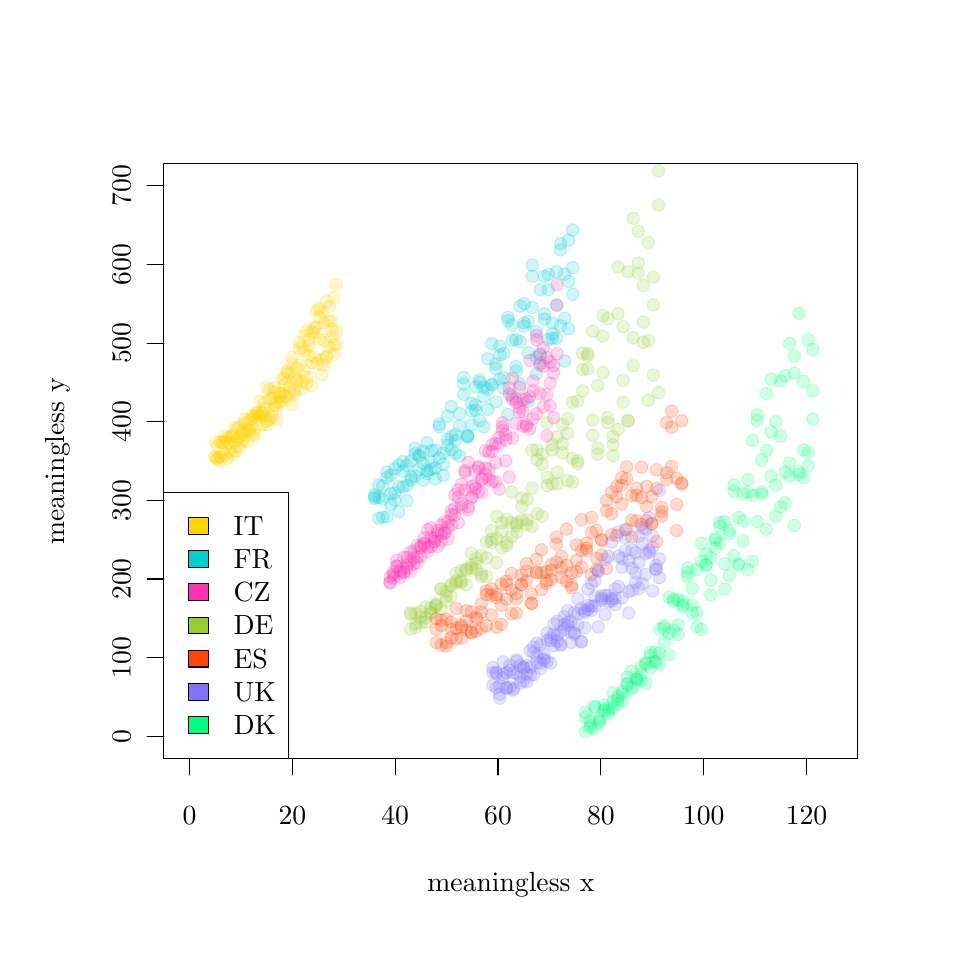
\begin{tikzpicture}[x=1pt,y=1pt]
\definecolor[named]{drawColor}{rgb}{0.00,0.00,0.00}
\definecolor[named]{fillColor}{rgb}{1.00,1.00,1.00}
\fill[color=fillColor,] (0,0) rectangle (325.21,325.21);
\begin{scope}
\path[clip] (  0.00,  0.00) rectangle (325.21,325.21);
\definecolor[named]{drawColor}{rgb}{0.09,0.00,0.33}
\definecolor[named]{drawColor}{rgb}{0.00,0.00,0.00}

\draw[color=drawColor,line cap=round,line join=round,fill opacity=0.00,] ( 58.49, 61.20) -- (281.44, 61.20);

\draw[color=drawColor,line cap=round,line join=round,fill opacity=0.00,] ( 58.49, 61.20) -- ( 58.49, 55.20);

\draw[color=drawColor,line cap=round,line join=round,fill opacity=0.00,] ( 95.65, 61.20) -- ( 95.65, 55.20);

\draw[color=drawColor,line cap=round,line join=round,fill opacity=0.00,] (132.80, 61.20) -- (132.80, 55.20);

\draw[color=drawColor,line cap=round,line join=round,fill opacity=0.00,] (169.96, 61.20) -- (169.96, 55.20);

\draw[color=drawColor,line cap=round,line join=round,fill opacity=0.00,] (207.12, 61.20) -- (207.12, 55.20);

\draw[color=drawColor,line cap=round,line join=round,fill opacity=0.00,] (244.28, 61.20) -- (244.28, 55.20);

\draw[color=drawColor,line cap=round,line join=round,fill opacity=0.00,] (281.44, 61.20) -- (281.44, 55.20);

\node[color=drawColor,anchor=base,inner sep=0pt, outer sep=0pt, scale=  1.00] at ( 58.49, 37.20) {0%
};

\node[color=drawColor,anchor=base,inner sep=0pt, outer sep=0pt, scale=  1.00] at ( 95.65, 37.20) {20%
};

\node[color=drawColor,anchor=base,inner sep=0pt, outer sep=0pt, scale=  1.00] at (132.80, 37.20) {40%
};

\node[color=drawColor,anchor=base,inner sep=0pt, outer sep=0pt, scale=  1.00] at (169.96, 37.20) {60%
};

\node[color=drawColor,anchor=base,inner sep=0pt, outer sep=0pt, scale=  1.00] at (207.12, 37.20) {80%
};

\node[color=drawColor,anchor=base,inner sep=0pt, outer sep=0pt, scale=  1.00] at (244.28, 37.20) {100%
};

\node[color=drawColor,anchor=base,inner sep=0pt, outer sep=0pt, scale=  1.00] at (281.44, 37.20) {120%
};

\draw[color=drawColor,line cap=round,line join=round,fill opacity=0.00,] ( 49.20, 69.16) -- ( 49.20,268.06);

\draw[color=drawColor,line cap=round,line join=round,fill opacity=0.00,] ( 49.20, 69.16) -- ( 43.20, 69.16);

\draw[color=drawColor,line cap=round,line join=round,fill opacity=0.00,] ( 49.20, 97.57) -- ( 43.20, 97.57);

\draw[color=drawColor,line cap=round,line join=round,fill opacity=0.00,] ( 49.20,125.99) -- ( 43.20,125.99);

\draw[color=drawColor,line cap=round,line join=round,fill opacity=0.00,] ( 49.20,154.40) -- ( 43.20,154.40);

\draw[color=drawColor,line cap=round,line join=round,fill opacity=0.00,] ( 49.20,182.81) -- ( 43.20,182.81);

\draw[color=drawColor,line cap=round,line join=round,fill opacity=0.00,] ( 49.20,211.23) -- ( 43.20,211.23);

\draw[color=drawColor,line cap=round,line join=round,fill opacity=0.00,] ( 49.20,239.64) -- ( 43.20,239.64);

\draw[color=drawColor,line cap=round,line join=round,fill opacity=0.00,] ( 49.20,268.06) -- ( 43.20,268.06);

\node[rotate= 90.00,color=drawColor,anchor=base,inner sep=0pt, outer sep=0pt, scale=  1.00] at ( 37.20, 69.16) {0%
};

\node[rotate= 90.00,color=drawColor,anchor=base,inner sep=0pt, outer sep=0pt, scale=  1.00] at ( 37.20, 97.57) {100%
};

\node[rotate= 90.00,color=drawColor,anchor=base,inner sep=0pt, outer sep=0pt, scale=  1.00] at ( 37.20,125.99) {200%
};

\node[rotate= 90.00,color=drawColor,anchor=base,inner sep=0pt, outer sep=0pt, scale=  1.00] at ( 37.20,154.40) {300%
};

\node[rotate= 90.00,color=drawColor,anchor=base,inner sep=0pt, outer sep=0pt, scale=  1.00] at ( 37.20,182.81) {400%
};

\node[rotate= 90.00,color=drawColor,anchor=base,inner sep=0pt, outer sep=0pt, scale=  1.00] at ( 37.20,211.23) {500%
};

\node[rotate= 90.00,color=drawColor,anchor=base,inner sep=0pt, outer sep=0pt, scale=  1.00] at ( 37.20,239.64) {600%
};

\node[rotate= 90.00,color=drawColor,anchor=base,inner sep=0pt, outer sep=0pt, scale=  1.00] at ( 37.20,268.06) {700%
};

\draw[color=drawColor,line cap=round,line join=round,fill opacity=0.00,] ( 49.20, 61.20) --
	(300.01, 61.20) --
	(300.01,276.01) --
	( 49.20,276.01) --
	( 49.20, 61.20);
\end{scope}
\begin{scope}
\path[clip] (  0.00,  0.00) rectangle (325.21,325.21);
\definecolor[named]{drawColor}{rgb}{0.09,0.00,0.33}
\definecolor[named]{drawColor}{rgb}{0.00,0.00,0.00}

\node[color=drawColor,anchor=base,inner sep=0pt, outer sep=0pt, scale=  1.00] at (174.61, 13.20) {meaningless x%
};

\node[rotate= 90.00,color=drawColor,anchor=base,inner sep=0pt, outer sep=0pt, scale=  1.00] at ( 13.20,168.61) {meaningless y%
};
\end{scope}
\begin{scope}
\path[clip] ( 49.20, 61.20) rectangle (300.01,276.01);
\definecolor[named]{drawColor}{rgb}{0.09,0.00,0.33}
\definecolor[named]{drawColor}{rgb}{1.00,0.84,0.00}
\definecolor[named]{fillColor}{rgb}{1.00,0.84,0.00}

\draw[color=drawColor,line cap=round,line join=round,fill=fillColor,fill opacity=0.19,draw opacity=0.19,] ( 67.78,170.07) circle (  2.25);

\draw[color=drawColor,line cap=round,line join=round,fill=fillColor,fill opacity=0.19,draw opacity=0.19,] ( 68.67,169.52) circle (  2.25);

\draw[color=drawColor,line cap=round,line join=round,fill=fillColor,fill opacity=0.19,draw opacity=0.19,] ( 69.57,170.04) circle (  2.25);

\draw[color=drawColor,line cap=round,line join=round,fill=fillColor,fill opacity=0.19,draw opacity=0.19,] ( 70.46,171.54) circle (  2.25);

\draw[color=drawColor,line cap=round,line join=round,fill=fillColor,fill opacity=0.19,draw opacity=0.19,] ( 71.36,175.95) circle (  2.25);

\draw[color=drawColor,line cap=round,line join=round,fill=fillColor,fill opacity=0.19,draw opacity=0.19,] ( 72.25,176.72) circle (  2.25);

\draw[color=drawColor,line cap=round,line join=round,fill=fillColor,fill opacity=0.19,draw opacity=0.19,] ( 73.14,171.70) circle (  2.25);

\draw[color=drawColor,line cap=round,line join=round,fill=fillColor,fill opacity=0.19,draw opacity=0.19,] ( 74.04,177.81) circle (  2.25);

\draw[color=drawColor,line cap=round,line join=round,fill=fillColor,fill opacity=0.19,draw opacity=0.19,] ( 74.93,180.69) circle (  2.25);

\draw[color=drawColor,line cap=round,line join=round,fill=fillColor,fill opacity=0.19,draw opacity=0.19,] ( 75.83,176.29) circle (  2.25);

\draw[color=drawColor,line cap=round,line join=round,fill=fillColor,fill opacity=0.19,draw opacity=0.19,] ( 76.72,181.26) circle (  2.25);

\draw[color=drawColor,line cap=round,line join=round,fill=fillColor,fill opacity=0.19,draw opacity=0.19,] ( 77.62,178.55) circle (  2.25);

\draw[color=drawColor,line cap=round,line join=round,fill=fillColor,fill opacity=0.19,draw opacity=0.19,] ( 78.51,182.45) circle (  2.25);

\draw[color=drawColor,line cap=round,line join=round,fill=fillColor,fill opacity=0.19,draw opacity=0.19,] ( 79.40,181.91) circle (  2.25);

\draw[color=drawColor,line cap=round,line join=round,fill=fillColor,fill opacity=0.19,draw opacity=0.19,] ( 80.30,179.85) circle (  2.25);

\draw[color=drawColor,line cap=round,line join=round,fill=fillColor,fill opacity=0.19,draw opacity=0.19,] ( 81.19,185.24) circle (  2.25);

\draw[color=drawColor,line cap=round,line join=round,fill=fillColor,fill opacity=0.19,draw opacity=0.19,] ( 82.09,184.92) circle (  2.25);

\draw[color=drawColor,line cap=round,line join=round,fill=fillColor,fill opacity=0.19,draw opacity=0.19,] ( 82.98,185.23) circle (  2.25);

\draw[color=drawColor,line cap=round,line join=round,fill=fillColor,fill opacity=0.19,draw opacity=0.19,] ( 83.87,185.23) circle (  2.25);

\draw[color=drawColor,line cap=round,line join=round,fill=fillColor,fill opacity=0.19,draw opacity=0.19,] ( 84.77,186.27) circle (  2.25);

\draw[color=drawColor,line cap=round,line join=round,fill=fillColor,fill opacity=0.19,draw opacity=0.19,] ( 85.66,189.92) circle (  2.25);

\draw[color=drawColor,line cap=round,line join=round,fill=fillColor,fill opacity=0.19,draw opacity=0.19,] ( 86.56,195.08) circle (  2.25);

\draw[color=drawColor,line cap=round,line join=round,fill=fillColor,fill opacity=0.19,draw opacity=0.19,] ( 87.45,183.59) circle (  2.25);

\draw[color=drawColor,line cap=round,line join=round,fill=fillColor,fill opacity=0.19,draw opacity=0.19,] ( 88.35,191.36) circle (  2.25);

\draw[color=drawColor,line cap=round,line join=round,fill=fillColor,fill opacity=0.19,draw opacity=0.19,] ( 89.24,195.07) circle (  2.25);

\draw[color=drawColor,line cap=round,line join=round,fill=fillColor,fill opacity=0.19,draw opacity=0.19,] ( 90.13,188.45) circle (  2.25);

\draw[color=drawColor,line cap=round,line join=round,fill=fillColor,fill opacity=0.19,draw opacity=0.19,] ( 91.03,193.10) circle (  2.25);

\draw[color=drawColor,line cap=round,line join=round,fill=fillColor,fill opacity=0.19,draw opacity=0.19,] ( 91.92,198.51) circle (  2.25);

\draw[color=drawColor,line cap=round,line join=round,fill=fillColor,fill opacity=0.19,draw opacity=0.19,] ( 92.82,196.27) circle (  2.25);

\draw[color=drawColor,line cap=round,line join=round,fill=fillColor,fill opacity=0.19,draw opacity=0.19,] ( 93.71,191.59) circle (  2.25);

\draw[color=drawColor,line cap=round,line join=round,fill=fillColor,fill opacity=0.19,draw opacity=0.19,] ( 94.61,193.56) circle (  2.25);

\draw[color=drawColor,line cap=round,line join=round,fill=fillColor,fill opacity=0.19,draw opacity=0.19,] ( 95.50,206.14) circle (  2.25);

\draw[color=drawColor,line cap=round,line join=round,fill=fillColor,fill opacity=0.19,draw opacity=0.19,] ( 96.39,192.68) circle (  2.25);

\draw[color=drawColor,line cap=round,line join=round,fill=fillColor,fill opacity=0.19,draw opacity=0.19,] ( 97.29,197.94) circle (  2.25);

\draw[color=drawColor,line cap=round,line join=round,fill=fillColor,fill opacity=0.19,draw opacity=0.19,] ( 98.18,209.29) circle (  2.25);

\draw[color=drawColor,line cap=round,line join=round,fill=fillColor,fill opacity=0.19,draw opacity=0.19,] ( 99.08,194.66) circle (  2.25);

\draw[color=drawColor,line cap=round,line join=round,fill=fillColor,fill opacity=0.19,draw opacity=0.19,] ( 99.97,208.52) circle (  2.25);

\draw[color=drawColor,line cap=round,line join=round,fill=fillColor,fill opacity=0.19,draw opacity=0.19,] (100.86,198.95) circle (  2.25);

\draw[color=drawColor,line cap=round,line join=round,fill=fillColor,fill opacity=0.19,draw opacity=0.19,] (101.76,206.67) circle (  2.25);

\draw[color=drawColor,line cap=round,line join=round,fill=fillColor,fill opacity=0.19,draw opacity=0.19,] (102.65,195.77) circle (  2.25);

\draw[color=drawColor,line cap=round,line join=round,fill=fillColor,fill opacity=0.19,draw opacity=0.19,] (103.55,216.74) circle (  2.25);

\draw[color=drawColor,line cap=round,line join=round,fill=fillColor,fill opacity=0.19,draw opacity=0.19,] (104.44,223.15) circle (  2.25);

\draw[color=drawColor,line cap=round,line join=round,fill=fillColor,fill opacity=0.19,draw opacity=0.19,] (105.34,220.64) circle (  2.25);

\draw[color=drawColor,line cap=round,line join=round,fill=fillColor,fill opacity=0.19,draw opacity=0.19,] (106.23,205.27) circle (  2.25);

\draw[color=drawColor,line cap=round,line join=round,fill=fillColor,fill opacity=0.19,draw opacity=0.19,] (107.12,218.51) circle (  2.25);

\draw[color=drawColor,line cap=round,line join=round,fill=fillColor,fill opacity=0.19,draw opacity=0.19,] (108.02,206.09) circle (  2.25);

\draw[color=drawColor,line cap=round,line join=round,fill=fillColor,fill opacity=0.19,draw opacity=0.19,] (108.91,219.19) circle (  2.25);

\draw[color=drawColor,line cap=round,line join=round,fill=fillColor,fill opacity=0.19,draw opacity=0.19,] (109.81,213.53) circle (  2.25);

\draw[color=drawColor,line cap=round,line join=round,fill=fillColor,fill opacity=0.19,draw opacity=0.19,] (110.70,207.11) circle (  2.25);

\draw[color=drawColor,line cap=round,line join=round,fill=fillColor,fill opacity=0.19,draw opacity=0.19,] (111.60,210.53) circle (  2.25);

\draw[color=drawColor,line cap=round,line join=round,fill=fillColor,fill opacity=0.19,draw opacity=0.19,] ( 67.78,175.54) circle (  2.25);

\draw[color=drawColor,line cap=round,line join=round,fill=fillColor,fill opacity=0.19,draw opacity=0.19,] ( 68.67,174.10) circle (  2.25);

\draw[color=drawColor,line cap=round,line join=round,fill=fillColor,fill opacity=0.19,draw opacity=0.19,] ( 69.57,168.60) circle (  2.25);

\draw[color=drawColor,line cap=round,line join=round,fill=fillColor,fill opacity=0.19,draw opacity=0.19,] ( 70.46,175.23) circle (  2.25);

\draw[color=drawColor,line cap=round,line join=round,fill=fillColor,fill opacity=0.19,draw opacity=0.19,] ( 71.36,177.57) circle (  2.25);

\draw[color=drawColor,line cap=round,line join=round,fill=fillColor,fill opacity=0.19,draw opacity=0.19,] ( 72.25,175.36) circle (  2.25);

\draw[color=drawColor,line cap=round,line join=round,fill=fillColor,fill opacity=0.19,draw opacity=0.19,] ( 73.14,175.00) circle (  2.25);

\draw[color=drawColor,line cap=round,line join=round,fill=fillColor,fill opacity=0.19,draw opacity=0.19,] ( 74.04,177.58) circle (  2.25);

\draw[color=drawColor,line cap=round,line join=round,fill=fillColor,fill opacity=0.19,draw opacity=0.19,] ( 74.93,172.14) circle (  2.25);

\draw[color=drawColor,line cap=round,line join=round,fill=fillColor,fill opacity=0.19,draw opacity=0.19,] ( 75.83,173.71) circle (  2.25);

\draw[color=drawColor,line cap=round,line join=round,fill=fillColor,fill opacity=0.19,draw opacity=0.19,] ( 76.72,173.63) circle (  2.25);

\draw[color=drawColor,line cap=round,line join=round,fill=fillColor,fill opacity=0.19,draw opacity=0.19,] ( 77.62,179.32) circle (  2.25);

\draw[color=drawColor,line cap=round,line join=round,fill=fillColor,fill opacity=0.19,draw opacity=0.19,] ( 78.51,177.97) circle (  2.25);

\draw[color=drawColor,line cap=round,line join=round,fill=fillColor,fill opacity=0.19,draw opacity=0.19,] ( 79.40,175.60) circle (  2.25);

\draw[color=drawColor,line cap=round,line join=round,fill=fillColor,fill opacity=0.19,draw opacity=0.19,] ( 80.30,183.55) circle (  2.25);

\draw[color=drawColor,line cap=round,line join=round,fill=fillColor,fill opacity=0.19,draw opacity=0.19,] ( 81.19,177.85) circle (  2.25);

\draw[color=drawColor,line cap=round,line join=round,fill=fillColor,fill opacity=0.19,draw opacity=0.19,] ( 82.09,180.07) circle (  2.25);

\draw[color=drawColor,line cap=round,line join=round,fill=fillColor,fill opacity=0.19,draw opacity=0.19,] ( 82.98,186.14) circle (  2.25);

\draw[color=drawColor,line cap=round,line join=round,fill=fillColor,fill opacity=0.19,draw opacity=0.19,] ( 83.87,190.21) circle (  2.25);

\draw[color=drawColor,line cap=round,line join=round,fill=fillColor,fill opacity=0.19,draw opacity=0.19,] ( 84.77,185.80) circle (  2.25);

\draw[color=drawColor,line cap=round,line join=round,fill=fillColor,fill opacity=0.19,draw opacity=0.19,] ( 85.66,184.69) circle (  2.25);

\draw[color=drawColor,line cap=round,line join=round,fill=fillColor,fill opacity=0.19,draw opacity=0.19,] ( 86.56,181.69) circle (  2.25);

\draw[color=drawColor,line cap=round,line join=round,fill=fillColor,fill opacity=0.19,draw opacity=0.19,] ( 87.45,194.35) circle (  2.25);

\draw[color=drawColor,line cap=round,line join=round,fill=fillColor,fill opacity=0.19,draw opacity=0.19,] ( 88.35,184.59) circle (  2.25);

\draw[color=drawColor,line cap=round,line join=round,fill=fillColor,fill opacity=0.19,draw opacity=0.19,] ( 89.24,188.65) circle (  2.25);

\draw[color=drawColor,line cap=round,line join=round,fill=fillColor,fill opacity=0.19,draw opacity=0.19,] ( 90.13,183.54) circle (  2.25);

\draw[color=drawColor,line cap=round,line join=round,fill=fillColor,fill opacity=0.19,draw opacity=0.19,] ( 91.03,189.81) circle (  2.25);

\draw[color=drawColor,line cap=round,line join=round,fill=fillColor,fill opacity=0.19,draw opacity=0.19,] ( 91.92,193.02) circle (  2.25);

\draw[color=drawColor,line cap=round,line join=round,fill=fillColor,fill opacity=0.19,draw opacity=0.19,] ( 92.82,198.23) circle (  2.25);

\draw[color=drawColor,line cap=round,line join=round,fill=fillColor,fill opacity=0.19,draw opacity=0.19,] ( 93.71,201.16) circle (  2.25);

\draw[color=drawColor,line cap=round,line join=round,fill=fillColor,fill opacity=0.19,draw opacity=0.19,] ( 94.61,200.42) circle (  2.25);

\draw[color=drawColor,line cap=round,line join=round,fill=fillColor,fill opacity=0.19,draw opacity=0.19,] ( 95.50,189.06) circle (  2.25);

\draw[color=drawColor,line cap=round,line join=round,fill=fillColor,fill opacity=0.19,draw opacity=0.19,] ( 96.39,193.97) circle (  2.25);

\draw[color=drawColor,line cap=round,line join=round,fill=fillColor,fill opacity=0.19,draw opacity=0.19,] ( 97.29,197.34) circle (  2.25);

\draw[color=drawColor,line cap=round,line join=round,fill=fillColor,fill opacity=0.19,draw opacity=0.19,] ( 98.18,211.56) circle (  2.25);

\draw[color=drawColor,line cap=round,line join=round,fill=fillColor,fill opacity=0.19,draw opacity=0.19,] ( 99.08,197.24) circle (  2.25);

\draw[color=drawColor,line cap=round,line join=round,fill=fillColor,fill opacity=0.19,draw opacity=0.19,] ( 99.97,214.05) circle (  2.25);

\draw[color=drawColor,line cap=round,line join=round,fill=fillColor,fill opacity=0.19,draw opacity=0.19,] (100.86,215.81) circle (  2.25);

\draw[color=drawColor,line cap=round,line join=round,fill=fillColor,fill opacity=0.19,draw opacity=0.19,] (101.76,212.45) circle (  2.25);

\draw[color=drawColor,line cap=round,line join=round,fill=fillColor,fill opacity=0.19,draw opacity=0.19,] (102.65,215.21) circle (  2.25);

\draw[color=drawColor,line cap=round,line join=round,fill=fillColor,fill opacity=0.19,draw opacity=0.19,] (103.55,206.27) circle (  2.25);

\draw[color=drawColor,line cap=round,line join=round,fill=fillColor,fill opacity=0.19,draw opacity=0.19,] (104.44,203.85) circle (  2.25);

\draw[color=drawColor,line cap=round,line join=round,fill=fillColor,fill opacity=0.19,draw opacity=0.19,] (105.34,212.64) circle (  2.25);

\draw[color=drawColor,line cap=round,line join=round,fill=fillColor,fill opacity=0.19,draw opacity=0.19,] (106.23,199.82) circle (  2.25);

\draw[color=drawColor,line cap=round,line join=round,fill=fillColor,fill opacity=0.19,draw opacity=0.19,] (107.12,212.15) circle (  2.25);

\draw[color=drawColor,line cap=round,line join=round,fill=fillColor,fill opacity=0.19,draw opacity=0.19,] (108.02,226.32) circle (  2.25);

\draw[color=drawColor,line cap=round,line join=round,fill=fillColor,fill opacity=0.19,draw opacity=0.19,] (108.91,224.45) circle (  2.25);

\draw[color=drawColor,line cap=round,line join=round,fill=fillColor,fill opacity=0.19,draw opacity=0.19,] (109.81,216.16) circle (  2.25);

\draw[color=drawColor,line cap=round,line join=round,fill=fillColor,fill opacity=0.19,draw opacity=0.19,] (110.70,227.70) circle (  2.25);

\draw[color=drawColor,line cap=round,line join=round,fill=fillColor,fill opacity=0.19,draw opacity=0.19,] (111.60,215.41) circle (  2.25);

\draw[color=drawColor,line cap=round,line join=round,fill=fillColor,fill opacity=0.19,draw opacity=0.19,] ( 67.78,170.07) circle (  2.25);

\draw[color=drawColor,line cap=round,line join=round,fill=fillColor,fill opacity=0.19,draw opacity=0.19,] ( 68.67,169.40) circle (  2.25);

\draw[color=drawColor,line cap=round,line join=round,fill=fillColor,fill opacity=0.19,draw opacity=0.19,] ( 69.57,175.55) circle (  2.25);

\draw[color=drawColor,line cap=round,line join=round,fill=fillColor,fill opacity=0.19,draw opacity=0.19,] ( 70.46,175.35) circle (  2.25);

\draw[color=drawColor,line cap=round,line join=round,fill=fillColor,fill opacity=0.19,draw opacity=0.19,] ( 71.36,171.02) circle (  2.25);

\draw[color=drawColor,line cap=round,line join=round,fill=fillColor,fill opacity=0.19,draw opacity=0.19,] ( 72.25,169.64) circle (  2.25);

\draw[color=drawColor,line cap=round,line join=round,fill=fillColor,fill opacity=0.19,draw opacity=0.19,] ( 73.14,177.35) circle (  2.25);

\draw[color=drawColor,line cap=round,line join=round,fill=fillColor,fill opacity=0.19,draw opacity=0.19,] ( 74.04,170.91) circle (  2.25);

\draw[color=drawColor,line cap=round,line join=round,fill=fillColor,fill opacity=0.19,draw opacity=0.19,] ( 74.93,175.63) circle (  2.25);

\draw[color=drawColor,line cap=round,line join=round,fill=fillColor,fill opacity=0.19,draw opacity=0.19,] ( 75.83,180.48) circle (  2.25);

\draw[color=drawColor,line cap=round,line join=round,fill=fillColor,fill opacity=0.19,draw opacity=0.19,] ( 76.72,177.29) circle (  2.25);

\draw[color=drawColor,line cap=round,line join=round,fill=fillColor,fill opacity=0.19,draw opacity=0.19,] ( 77.62,176.08) circle (  2.25);

\draw[color=drawColor,line cap=round,line join=round,fill=fillColor,fill opacity=0.19,draw opacity=0.19,] ( 78.51,183.73) circle (  2.25);

\draw[color=drawColor,line cap=round,line join=round,fill=fillColor,fill opacity=0.19,draw opacity=0.19,] ( 79.40,179.65) circle (  2.25);

\draw[color=drawColor,line cap=round,line join=round,fill=fillColor,fill opacity=0.19,draw opacity=0.19,] ( 80.30,180.93) circle (  2.25);

\draw[color=drawColor,line cap=round,line join=round,fill=fillColor,fill opacity=0.19,draw opacity=0.19,] ( 81.19,183.94) circle (  2.25);

\draw[color=drawColor,line cap=round,line join=round,fill=fillColor,fill opacity=0.19,draw opacity=0.19,] ( 82.09,178.21) circle (  2.25);

\draw[color=drawColor,line cap=round,line join=round,fill=fillColor,fill opacity=0.19,draw opacity=0.19,] ( 82.98,185.91) circle (  2.25);

\draw[color=drawColor,line cap=round,line join=round,fill=fillColor,fill opacity=0.19,draw opacity=0.19,] ( 83.87,184.35) circle (  2.25);

\draw[color=drawColor,line cap=round,line join=round,fill=fillColor,fill opacity=0.19,draw opacity=0.19,] ( 84.77,181.69) circle (  2.25);

\draw[color=drawColor,line cap=round,line join=round,fill=fillColor,fill opacity=0.19,draw opacity=0.19,] ( 85.66,187.52) circle (  2.25);

\draw[color=drawColor,line cap=round,line join=round,fill=fillColor,fill opacity=0.19,draw opacity=0.19,] ( 86.56,182.93) circle (  2.25);

\draw[color=drawColor,line cap=round,line join=round,fill=fillColor,fill opacity=0.19,draw opacity=0.19,] ( 87.45,190.97) circle (  2.25);

\draw[color=drawColor,line cap=round,line join=round,fill=fillColor,fill opacity=0.19,draw opacity=0.19,] ( 88.35,186.04) circle (  2.25);

\draw[color=drawColor,line cap=round,line join=round,fill=fillColor,fill opacity=0.19,draw opacity=0.19,] ( 89.24,193.40) circle (  2.25);

\draw[color=drawColor,line cap=round,line join=round,fill=fillColor,fill opacity=0.19,draw opacity=0.19,] ( 90.13,190.07) circle (  2.25);

\draw[color=drawColor,line cap=round,line join=round,fill=fillColor,fill opacity=0.19,draw opacity=0.19,] ( 91.03,192.01) circle (  2.25);

\draw[color=drawColor,line cap=round,line join=round,fill=fillColor,fill opacity=0.19,draw opacity=0.19,] ( 91.92,190.34) circle (  2.25);

\draw[color=drawColor,line cap=round,line join=round,fill=fillColor,fill opacity=0.19,draw opacity=0.19,] ( 92.82,192.18) circle (  2.25);

\draw[color=drawColor,line cap=round,line join=round,fill=fillColor,fill opacity=0.19,draw opacity=0.19,] ( 93.71,200.78) circle (  2.25);

\draw[color=drawColor,line cap=round,line join=round,fill=fillColor,fill opacity=0.19,draw opacity=0.19,] ( 94.61,195.23) circle (  2.25);

\draw[color=drawColor,line cap=round,line join=round,fill=fillColor,fill opacity=0.19,draw opacity=0.19,] ( 95.50,203.62) circle (  2.25);

\draw[color=drawColor,line cap=round,line join=round,fill=fillColor,fill opacity=0.19,draw opacity=0.19,] ( 96.39,198.81) circle (  2.25);

\draw[color=drawColor,line cap=round,line join=round,fill=fillColor,fill opacity=0.19,draw opacity=0.19,] ( 97.29,202.13) circle (  2.25);

\draw[color=drawColor,line cap=round,line join=round,fill=fillColor,fill opacity=0.19,draw opacity=0.19,] ( 98.18,203.30) circle (  2.25);

\draw[color=drawColor,line cap=round,line join=round,fill=fillColor,fill opacity=0.19,draw opacity=0.19,] ( 99.08,209.61) circle (  2.25);

\draw[color=drawColor,line cap=round,line join=round,fill=fillColor,fill opacity=0.19,draw opacity=0.19,] ( 99.97,201.46) circle (  2.25);

\draw[color=drawColor,line cap=round,line join=round,fill=fillColor,fill opacity=0.19,draw opacity=0.19,] (100.86,196.83) circle (  2.25);

\draw[color=drawColor,line cap=round,line join=round,fill=fillColor,fill opacity=0.19,draw opacity=0.19,] (101.76,210.24) circle (  2.25);

\draw[color=drawColor,line cap=round,line join=round,fill=fillColor,fill opacity=0.19,draw opacity=0.19,] (102.65,204.15) circle (  2.25);

\draw[color=drawColor,line cap=round,line join=round,fill=fillColor,fill opacity=0.19,draw opacity=0.19,] (103.55,215.00) circle (  2.25);

\draw[color=drawColor,line cap=round,line join=round,fill=fillColor,fill opacity=0.19,draw opacity=0.19,] (104.44,217.01) circle (  2.25);

\draw[color=drawColor,line cap=round,line join=round,fill=fillColor,fill opacity=0.19,draw opacity=0.19,] (105.34,223.69) circle (  2.25);

\draw[color=drawColor,line cap=round,line join=round,fill=fillColor,fill opacity=0.19,draw opacity=0.19,] (106.23,222.64) circle (  2.25);

\draw[color=drawColor,line cap=round,line join=round,fill=fillColor,fill opacity=0.19,draw opacity=0.19,] (107.12,203.27) circle (  2.25);

\draw[color=drawColor,line cap=round,line join=round,fill=fillColor,fill opacity=0.19,draw opacity=0.19,] (108.02,206.61) circle (  2.25);

\draw[color=drawColor,line cap=round,line join=round,fill=fillColor,fill opacity=0.19,draw opacity=0.19,] (108.91,209.73) circle (  2.25);

\draw[color=drawColor,line cap=round,line join=round,fill=fillColor,fill opacity=0.19,draw opacity=0.19,] (109.81,219.21) circle (  2.25);

\draw[color=drawColor,line cap=round,line join=round,fill=fillColor,fill opacity=0.19,draw opacity=0.19,] (110.70,210.70) circle (  2.25);

\draw[color=drawColor,line cap=round,line join=round,fill=fillColor,fill opacity=0.19,draw opacity=0.19,] (111.60,232.38) circle (  2.25);
\definecolor[named]{drawColor}{rgb}{0.00,0.81,0.82}
\definecolor[named]{fillColor}{rgb}{0.00,0.81,0.82}

\draw[color=drawColor,line cap=round,line join=round,fill=fillColor,fill opacity=0.19,draw opacity=0.19,] (125.37,155.16) circle (  2.25);

\draw[color=drawColor,line cap=round,line join=round,fill=fillColor,fill opacity=0.19,draw opacity=0.19,] (126.83,159.99) circle (  2.25);

\draw[color=drawColor,line cap=round,line join=round,fill=fillColor,fill opacity=0.19,draw opacity=0.19,] (128.29,159.59) circle (  2.25);

\draw[color=drawColor,line cap=round,line join=round,fill=fillColor,fill opacity=0.19,draw opacity=0.19,] (129.75,148.39) circle (  2.25);

\draw[color=drawColor,line cap=round,line join=round,fill=fillColor,fill opacity=0.19,draw opacity=0.19,] (131.21,163.44) circle (  2.25);

\draw[color=drawColor,line cap=round,line join=round,fill=fillColor,fill opacity=0.19,draw opacity=0.19,] (132.68,154.58) circle (  2.25);

\draw[color=drawColor,line cap=round,line join=round,fill=fillColor,fill opacity=0.19,draw opacity=0.19,] (134.14,150.31) circle (  2.25);

\draw[color=drawColor,line cap=round,line join=round,fill=fillColor,fill opacity=0.19,draw opacity=0.19,] (135.60,164.93) circle (  2.25);

\draw[color=drawColor,line cap=round,line join=round,fill=fillColor,fill opacity=0.19,draw opacity=0.19,] (137.06,154.27) circle (  2.25);

\draw[color=drawColor,line cap=round,line join=round,fill=fillColor,fill opacity=0.19,draw opacity=0.19,] (138.52,162.86) circle (  2.25);

\draw[color=drawColor,line cap=round,line join=round,fill=fillColor,fill opacity=0.19,draw opacity=0.19,] (139.98,171.25) circle (  2.25);

\draw[color=drawColor,line cap=round,line join=round,fill=fillColor,fill opacity=0.19,draw opacity=0.19,] (141.44,170.30) circle (  2.25);

\draw[color=drawColor,line cap=round,line join=round,fill=fillColor,fill opacity=0.19,draw opacity=0.19,] (142.90,167.74) circle (  2.25);

\draw[color=drawColor,line cap=round,line join=round,fill=fillColor,fill opacity=0.19,draw opacity=0.19,] (144.36,175.26) circle (  2.25);

\draw[color=drawColor,line cap=round,line join=round,fill=fillColor,fill opacity=0.19,draw opacity=0.19,] (145.82,165.65) circle (  2.25);

\draw[color=drawColor,line cap=round,line join=round,fill=fillColor,fill opacity=0.19,draw opacity=0.19,] (147.28,162.24) circle (  2.25);

\draw[color=drawColor,line cap=round,line join=round,fill=fillColor,fill opacity=0.19,draw opacity=0.19,] (148.74,180.98) circle (  2.25);

\draw[color=drawColor,line cap=round,line join=round,fill=fillColor,fill opacity=0.19,draw opacity=0.19,] (150.20,163.42) circle (  2.25);

\draw[color=drawColor,line cap=round,line join=round,fill=fillColor,fill opacity=0.19,draw opacity=0.19,] (151.66,176.50) circle (  2.25);

\draw[color=drawColor,line cap=round,line join=round,fill=fillColor,fill opacity=0.19,draw opacity=0.19,] (153.12,177.49) circle (  2.25);

\draw[color=drawColor,line cap=round,line join=round,fill=fillColor,fill opacity=0.19,draw opacity=0.19,] (154.58,176.08) circle (  2.25);

\draw[color=drawColor,line cap=round,line join=round,fill=fillColor,fill opacity=0.19,draw opacity=0.19,] (156.04,185.71) circle (  2.25);

\draw[color=drawColor,line cap=round,line join=round,fill=fillColor,fill opacity=0.19,draw opacity=0.19,] (157.50,196.39) circle (  2.25);

\draw[color=drawColor,line cap=round,line join=round,fill=fillColor,fill opacity=0.19,draw opacity=0.19,] (158.96,177.37) circle (  2.25);

\draw[color=drawColor,line cap=round,line join=round,fill=fillColor,fill opacity=0.19,draw opacity=0.19,] (160.42,181.74) circle (  2.25);

\draw[color=drawColor,line cap=round,line join=round,fill=fillColor,fill opacity=0.19,draw opacity=0.19,] (161.88,186.95) circle (  2.25);

\draw[color=drawColor,line cap=round,line join=round,fill=fillColor,fill opacity=0.19,draw opacity=0.19,] (163.34,183.23) circle (  2.25);

\draw[color=drawColor,line cap=round,line join=round,fill=fillColor,fill opacity=0.19,draw opacity=0.19,] (164.80,195.31) circle (  2.25);

\draw[color=drawColor,line cap=round,line join=round,fill=fillColor,fill opacity=0.19,draw opacity=0.19,] (166.26,187.28) circle (  2.25);

\draw[color=drawColor,line cap=round,line join=round,fill=fillColor,fill opacity=0.19,draw opacity=0.19,] (167.72,210.98) circle (  2.25);

\draw[color=drawColor,line cap=round,line join=round,fill=fillColor,fill opacity=0.19,draw opacity=0.19,] (169.18,189.96) circle (  2.25);

\draw[color=drawColor,line cap=round,line join=round,fill=fillColor,fill opacity=0.19,draw opacity=0.19,] (170.64,206.93) circle (  2.25);

\draw[color=drawColor,line cap=round,line join=round,fill=fillColor,fill opacity=0.19,draw opacity=0.19,] (172.10,207.52) circle (  2.25);

\draw[color=drawColor,line cap=round,line join=round,fill=fillColor,fill opacity=0.19,draw opacity=0.19,] (173.56,220.51) circle (  2.25);

\draw[color=drawColor,line cap=round,line join=round,fill=fillColor,fill opacity=0.19,draw opacity=0.19,] (175.02,191.97) circle (  2.25);

\draw[color=drawColor,line cap=round,line join=round,fill=fillColor,fill opacity=0.19,draw opacity=0.19,] (176.49,202.78) circle (  2.25);

\draw[color=drawColor,line cap=round,line join=round,fill=fillColor,fill opacity=0.19,draw opacity=0.19,] (177.95,211.80) circle (  2.25);

\draw[color=drawColor,line cap=round,line join=round,fill=fillColor,fill opacity=0.19,draw opacity=0.19,] (179.41,225.48) circle (  2.25);

\draw[color=drawColor,line cap=round,line join=round,fill=fillColor,fill opacity=0.19,draw opacity=0.19,] (180.87,207.75) circle (  2.25);

\draw[color=drawColor,line cap=round,line join=round,fill=fillColor,fill opacity=0.19,draw opacity=0.19,] (182.33,235.42) circle (  2.25);

\draw[color=drawColor,line cap=round,line join=round,fill=fillColor,fill opacity=0.19,draw opacity=0.19,] (183.79,206.00) circle (  2.25);

\draw[color=drawColor,line cap=round,line join=round,fill=fillColor,fill opacity=0.19,draw opacity=0.19,] (185.25,207.39) circle (  2.25);

\draw[color=drawColor,line cap=round,line join=round,fill=fillColor,fill opacity=0.19,draw opacity=0.19,] (186.71,219.88) circle (  2.25);

\draw[color=drawColor,line cap=round,line join=round,fill=fillColor,fill opacity=0.19,draw opacity=0.19,] (188.17,212.49) circle (  2.25);

\draw[color=drawColor,line cap=round,line join=round,fill=fillColor,fill opacity=0.19,draw opacity=0.19,] (189.63,213.00) circle (  2.25);

\draw[color=drawColor,line cap=round,line join=round,fill=fillColor,fill opacity=0.19,draw opacity=0.19,] (191.09,225.01) circle (  2.25);

\draw[color=drawColor,line cap=round,line join=round,fill=fillColor,fill opacity=0.19,draw opacity=0.19,] (192.55,244.88) circle (  2.25);

\draw[color=drawColor,line cap=round,line join=round,fill=fillColor,fill opacity=0.19,draw opacity=0.19,] (194.01,220.23) circle (  2.25);

\draw[color=drawColor,line cap=round,line join=round,fill=fillColor,fill opacity=0.19,draw opacity=0.19,] (195.47,248.45) circle (  2.25);

\draw[color=drawColor,line cap=round,line join=round,fill=fillColor,fill opacity=0.19,draw opacity=0.19,] (196.93,228.87) circle (  2.25);

\draw[color=drawColor,line cap=round,line join=round,fill=fillColor,fill opacity=0.19,draw opacity=0.19,] (125.37,156.42) circle (  2.25);

\draw[color=drawColor,line cap=round,line join=round,fill=fillColor,fill opacity=0.19,draw opacity=0.19,] (126.83,147.95) circle (  2.25);

\draw[color=drawColor,line cap=round,line join=round,fill=fillColor,fill opacity=0.19,draw opacity=0.19,] (128.29,154.79) circle (  2.25);

\draw[color=drawColor,line cap=round,line join=round,fill=fillColor,fill opacity=0.19,draw opacity=0.19,] (129.75,162.62) circle (  2.25);

\draw[color=drawColor,line cap=round,line join=round,fill=fillColor,fill opacity=0.19,draw opacity=0.19,] (131.21,152.97) circle (  2.25);

\draw[color=drawColor,line cap=round,line join=round,fill=fillColor,fill opacity=0.19,draw opacity=0.19,] (132.68,165.83) circle (  2.25);

\draw[color=drawColor,line cap=round,line join=round,fill=fillColor,fill opacity=0.19,draw opacity=0.19,] (134.14,159.38) circle (  2.25);

\draw[color=drawColor,line cap=round,line join=round,fill=fillColor,fill opacity=0.19,draw opacity=0.19,] (135.60,168.44) circle (  2.25);

\draw[color=drawColor,line cap=round,line join=round,fill=fillColor,fill opacity=0.19,draw opacity=0.19,] (137.06,159.79) circle (  2.25);

\draw[color=drawColor,line cap=round,line join=round,fill=fillColor,fill opacity=0.19,draw opacity=0.19,] (138.52,168.67) circle (  2.25);

\draw[color=drawColor,line cap=round,line join=round,fill=fillColor,fill opacity=0.19,draw opacity=0.19,] (139.98,163.14) circle (  2.25);

\draw[color=drawColor,line cap=round,line join=round,fill=fillColor,fill opacity=0.19,draw opacity=0.19,] (141.44,170.67) circle (  2.25);

\draw[color=drawColor,line cap=round,line join=round,fill=fillColor,fill opacity=0.19,draw opacity=0.19,] (142.90,172.07) circle (  2.25);

\draw[color=drawColor,line cap=round,line join=round,fill=fillColor,fill opacity=0.19,draw opacity=0.19,] (144.36,164.09) circle (  2.25);

\draw[color=drawColor,line cap=round,line join=round,fill=fillColor,fill opacity=0.19,draw opacity=0.19,] (145.82,172.40) circle (  2.25);

\draw[color=drawColor,line cap=round,line join=round,fill=fillColor,fill opacity=0.19,draw opacity=0.19,] (147.28,166.10) circle (  2.25);

\draw[color=drawColor,line cap=round,line join=round,fill=fillColor,fill opacity=0.19,draw opacity=0.19,] (148.74,181.90) circle (  2.25);

\draw[color=drawColor,line cap=round,line join=round,fill=fillColor,fill opacity=0.19,draw opacity=0.19,] (150.20,167.38) circle (  2.25);

\draw[color=drawColor,line cap=round,line join=round,fill=fillColor,fill opacity=0.19,draw opacity=0.19,] (151.66,174.23) circle (  2.25);

\draw[color=drawColor,line cap=round,line join=round,fill=fillColor,fill opacity=0.19,draw opacity=0.19,] (153.12,188.30) circle (  2.25);

\draw[color=drawColor,line cap=round,line join=round,fill=fillColor,fill opacity=0.19,draw opacity=0.19,] (154.58,178.19) circle (  2.25);

\draw[color=drawColor,line cap=round,line join=round,fill=fillColor,fill opacity=0.19,draw opacity=0.19,] (156.04,181.30) circle (  2.25);

\draw[color=drawColor,line cap=round,line join=round,fill=fillColor,fill opacity=0.19,draw opacity=0.19,] (157.50,192.69) circle (  2.25);

\draw[color=drawColor,line cap=round,line join=round,fill=fillColor,fill opacity=0.19,draw opacity=0.19,] (158.96,177.85) circle (  2.25);

\draw[color=drawColor,line cap=round,line join=round,fill=fillColor,fill opacity=0.19,draw opacity=0.19,] (160.42,189.46) circle (  2.25);

\draw[color=drawColor,line cap=round,line join=round,fill=fillColor,fill opacity=0.19,draw opacity=0.19,] (161.88,188.89) circle (  2.25);

\draw[color=drawColor,line cap=round,line join=round,fill=fillColor,fill opacity=0.19,draw opacity=0.19,] (163.34,197.02) circle (  2.25);

\draw[color=drawColor,line cap=round,line join=round,fill=fillColor,fill opacity=0.19,draw opacity=0.19,] (164.80,180.98) circle (  2.25);

\draw[color=drawColor,line cap=round,line join=round,fill=fillColor,fill opacity=0.19,draw opacity=0.19,] (166.26,205.56) circle (  2.25);

\draw[color=drawColor,line cap=round,line join=round,fill=fillColor,fill opacity=0.19,draw opacity=0.19,] (167.72,196.10) circle (  2.25);

\draw[color=drawColor,line cap=round,line join=round,fill=fillColor,fill opacity=0.19,draw opacity=0.19,] (169.18,203.69) circle (  2.25);

\draw[color=drawColor,line cap=round,line join=round,fill=fillColor,fill opacity=0.19,draw opacity=0.19,] (170.64,210.10) circle (  2.25);

\draw[color=drawColor,line cap=round,line join=round,fill=fillColor,fill opacity=0.19,draw opacity=0.19,] (172.10,194.83) circle (  2.25);

\draw[color=drawColor,line cap=round,line join=round,fill=fillColor,fill opacity=0.19,draw opacity=0.19,] (173.56,219.33) circle (  2.25);

\draw[color=drawColor,line cap=round,line join=round,fill=fillColor,fill opacity=0.19,draw opacity=0.19,] (175.02,217.80) circle (  2.25);

\draw[color=drawColor,line cap=round,line join=round,fill=fillColor,fill opacity=0.19,draw opacity=0.19,] (176.49,212.48) circle (  2.25);

\draw[color=drawColor,line cap=round,line join=round,fill=fillColor,fill opacity=0.19,draw opacity=0.19,] (177.95,196.42) circle (  2.25);

\draw[color=drawColor,line cap=round,line join=round,fill=fillColor,fill opacity=0.19,draw opacity=0.19,] (179.41,218.47) circle (  2.25);

\draw[color=drawColor,line cap=round,line join=round,fill=fillColor,fill opacity=0.19,draw opacity=0.19,] (180.87,219.04) circle (  2.25);

\draw[color=drawColor,line cap=round,line join=round,fill=fillColor,fill opacity=0.19,draw opacity=0.19,] (182.33,239.41) circle (  2.25);

\draw[color=drawColor,line cap=round,line join=round,fill=fillColor,fill opacity=0.19,draw opacity=0.19,] (183.79,200.13) circle (  2.25);

\draw[color=drawColor,line cap=round,line join=round,fill=fillColor,fill opacity=0.19,draw opacity=0.19,] (185.25,230.51) circle (  2.25);

\draw[color=drawColor,line cap=round,line join=round,fill=fillColor,fill opacity=0.19,draw opacity=0.19,] (186.71,235.36) circle (  2.25);

\draw[color=drawColor,line cap=round,line join=round,fill=fillColor,fill opacity=0.19,draw opacity=0.19,] (188.17,230.52) circle (  2.25);

\draw[color=drawColor,line cap=round,line join=round,fill=fillColor,fill opacity=0.19,draw opacity=0.19,] (189.63,218.51) circle (  2.25);

\draw[color=drawColor,line cap=round,line join=round,fill=fillColor,fill opacity=0.19,draw opacity=0.19,] (191.09,236.99) circle (  2.25);

\draw[color=drawColor,line cap=round,line join=round,fill=fillColor,fill opacity=0.19,draw opacity=0.19,] (192.55,247.18) circle (  2.25);

\draw[color=drawColor,line cap=round,line join=round,fill=fillColor,fill opacity=0.19,draw opacity=0.19,] (194.01,236.16) circle (  2.25);

\draw[color=drawColor,line cap=round,line join=round,fill=fillColor,fill opacity=0.19,draw opacity=0.19,] (195.47,216.39) circle (  2.25);

\draw[color=drawColor,line cap=round,line join=round,fill=fillColor,fill opacity=0.19,draw opacity=0.19,] (196.93,238.53) circle (  2.25);

\draw[color=drawColor,line cap=round,line join=round,fill=fillColor,fill opacity=0.19,draw opacity=0.19,] (125.37,155.66) circle (  2.25);

\draw[color=drawColor,line cap=round,line join=round,fill=fillColor,fill opacity=0.19,draw opacity=0.19,] (126.83,155.45) circle (  2.25);

\draw[color=drawColor,line cap=round,line join=round,fill=fillColor,fill opacity=0.19,draw opacity=0.19,] (128.29,148.41) circle (  2.25);

\draw[color=drawColor,line cap=round,line join=round,fill=fillColor,fill opacity=0.19,draw opacity=0.19,] (129.75,164.62) circle (  2.25);

\draw[color=drawColor,line cap=round,line join=round,fill=fillColor,fill opacity=0.19,draw opacity=0.19,] (131.21,156.82) circle (  2.25);

\draw[color=drawColor,line cap=round,line join=round,fill=fillColor,fill opacity=0.19,draw opacity=0.19,] (132.68,157.14) circle (  2.25);

\draw[color=drawColor,line cap=round,line join=round,fill=fillColor,fill opacity=0.19,draw opacity=0.19,] (134.14,167.17) circle (  2.25);

\draw[color=drawColor,line cap=round,line join=round,fill=fillColor,fill opacity=0.19,draw opacity=0.19,] (135.60,159.18) circle (  2.25);

\draw[color=drawColor,line cap=round,line join=round,fill=fillColor,fill opacity=0.19,draw opacity=0.19,] (137.06,167.04) circle (  2.25);

\draw[color=drawColor,line cap=round,line join=round,fill=fillColor,fill opacity=0.19,draw opacity=0.19,] (138.52,161.72) circle (  2.25);

\draw[color=drawColor,line cap=round,line join=round,fill=fillColor,fill opacity=0.19,draw opacity=0.19,] (139.98,173.23) circle (  2.25);

\draw[color=drawColor,line cap=round,line join=round,fill=fillColor,fill opacity=0.19,draw opacity=0.19,] (141.44,165.64) circle (  2.25);

\draw[color=drawColor,line cap=round,line join=round,fill=fillColor,fill opacity=0.19,draw opacity=0.19,] (142.90,161.71) circle (  2.25);

\draw[color=drawColor,line cap=round,line join=round,fill=fillColor,fill opacity=0.19,draw opacity=0.19,] (144.36,165.06) circle (  2.25);

\draw[color=drawColor,line cap=round,line join=round,fill=fillColor,fill opacity=0.19,draw opacity=0.19,] (145.82,168.31) circle (  2.25);

\draw[color=drawColor,line cap=round,line join=round,fill=fillColor,fill opacity=0.19,draw opacity=0.19,] (147.28,172.50) circle (  2.25);

\draw[color=drawColor,line cap=round,line join=round,fill=fillColor,fill opacity=0.19,draw opacity=0.19,] (148.74,169.68) circle (  2.25);

\draw[color=drawColor,line cap=round,line join=round,fill=fillColor,fill opacity=0.19,draw opacity=0.19,] (150.20,171.52) circle (  2.25);

\draw[color=drawColor,line cap=round,line join=round,fill=fillColor,fill opacity=0.19,draw opacity=0.19,] (151.66,184.84) circle (  2.25);

\draw[color=drawColor,line cap=round,line join=round,fill=fillColor,fill opacity=0.19,draw opacity=0.19,] (153.12,172.76) circle (  2.25);

\draw[color=drawColor,line cap=round,line join=round,fill=fillColor,fill opacity=0.19,draw opacity=0.19,] (154.58,171.46) circle (  2.25);

\draw[color=drawColor,line cap=round,line join=round,fill=fillColor,fill opacity=0.19,draw opacity=0.19,] (156.04,170.41) circle (  2.25);

\draw[color=drawColor,line cap=round,line join=round,fill=fillColor,fill opacity=0.19,draw opacity=0.19,] (157.50,198.79) circle (  2.25);

\draw[color=drawColor,line cap=round,line join=round,fill=fillColor,fill opacity=0.19,draw opacity=0.19,] (158.96,177.45) circle (  2.25);

\draw[color=drawColor,line cap=round,line join=round,fill=fillColor,fill opacity=0.19,draw opacity=0.19,] (160.42,186.70) circle (  2.25);

\draw[color=drawColor,line cap=round,line join=round,fill=fillColor,fill opacity=0.19,draw opacity=0.19,] (161.88,195.38) circle (  2.25);

\draw[color=drawColor,line cap=round,line join=round,fill=fillColor,fill opacity=0.19,draw opacity=0.19,] (163.34,197.89) circle (  2.25);

\draw[color=drawColor,line cap=round,line join=round,fill=fillColor,fill opacity=0.19,draw opacity=0.19,] (164.80,191.93) circle (  2.25);

\draw[color=drawColor,line cap=round,line join=round,fill=fillColor,fill opacity=0.19,draw opacity=0.19,] (166.26,194.59) circle (  2.25);

\draw[color=drawColor,line cap=round,line join=round,fill=fillColor,fill opacity=0.19,draw opacity=0.19,] (167.72,196.34) circle (  2.25);

\draw[color=drawColor,line cap=round,line join=round,fill=fillColor,fill opacity=0.19,draw opacity=0.19,] (169.18,202.03) circle (  2.25);

\draw[color=drawColor,line cap=round,line join=round,fill=fillColor,fill opacity=0.19,draw opacity=0.19,] (170.64,198.15) circle (  2.25);

\draw[color=drawColor,line cap=round,line join=round,fill=fillColor,fill opacity=0.19,draw opacity=0.19,] (172.10,198.73) circle (  2.25);

\draw[color=drawColor,line cap=round,line join=round,fill=fillColor,fill opacity=0.19,draw opacity=0.19,] (173.56,185.48) circle (  2.25);

\draw[color=drawColor,line cap=round,line join=round,fill=fillColor,fill opacity=0.19,draw opacity=0.19,] (175.02,212.23) circle (  2.25);

\draw[color=drawColor,line cap=round,line join=round,fill=fillColor,fill opacity=0.19,draw opacity=0.19,] (176.49,201.05) circle (  2.25);

\draw[color=drawColor,line cap=round,line join=round,fill=fillColor,fill opacity=0.19,draw opacity=0.19,] (177.95,224.59) circle (  2.25);

\draw[color=drawColor,line cap=round,line join=round,fill=fillColor,fill opacity=0.19,draw opacity=0.19,] (179.41,217.39) circle (  2.25);

\draw[color=drawColor,line cap=round,line join=round,fill=fillColor,fill opacity=0.19,draw opacity=0.19,] (180.87,190.19) circle (  2.25);

\draw[color=drawColor,line cap=round,line join=round,fill=fillColor,fill opacity=0.19,draw opacity=0.19,] (182.33,224.09) circle (  2.25);

\draw[color=drawColor,line cap=round,line join=round,fill=fillColor,fill opacity=0.19,draw opacity=0.19,] (183.79,215.32) circle (  2.25);

\draw[color=drawColor,line cap=round,line join=round,fill=fillColor,fill opacity=0.19,draw opacity=0.19,] (185.25,204.09) circle (  2.25);

\draw[color=drawColor,line cap=round,line join=round,fill=fillColor,fill opacity=0.19,draw opacity=0.19,] (186.71,221.77) circle (  2.25);

\draw[color=drawColor,line cap=round,line join=round,fill=fillColor,fill opacity=0.19,draw opacity=0.19,] (188.17,236.06) circle (  2.25);

\draw[color=drawColor,line cap=round,line join=round,fill=fillColor,fill opacity=0.19,draw opacity=0.19,] (189.63,214.59) circle (  2.25);

\draw[color=drawColor,line cap=round,line join=round,fill=fillColor,fill opacity=0.19,draw opacity=0.19,] (191.09,212.99) circle (  2.25);

\draw[color=drawColor,line cap=round,line join=round,fill=fillColor,fill opacity=0.19,draw opacity=0.19,] (192.55,217.49) circle (  2.25);

\draw[color=drawColor,line cap=round,line join=round,fill=fillColor,fill opacity=0.19,draw opacity=0.19,] (194.01,204.73) circle (  2.25);

\draw[color=drawColor,line cap=round,line join=round,fill=fillColor,fill opacity=0.19,draw opacity=0.19,] (195.47,233.50) circle (  2.25);

\draw[color=drawColor,line cap=round,line join=round,fill=fillColor,fill opacity=0.19,draw opacity=0.19,] (196.93,252.07) circle (  2.25);
\definecolor[named]{drawColor}{rgb}{1.00,0.20,0.70}
\definecolor[named]{fillColor}{rgb}{1.00,0.20,0.70}

\draw[color=drawColor,line cap=round,line join=round,fill=fillColor,fill opacity=0.19,draw opacity=0.19,] (130.95,124.86) circle (  2.25);

\draw[color=drawColor,line cap=round,line join=round,fill=fillColor,fill opacity=0.19,draw opacity=0.19,] (132.18,126.47) circle (  2.25);

\draw[color=drawColor,line cap=round,line join=round,fill=fillColor,fill opacity=0.19,draw opacity=0.19,] (133.41,132.75) circle (  2.25);

\draw[color=drawColor,line cap=round,line join=round,fill=fillColor,fill opacity=0.19,draw opacity=0.19,] (134.64,128.40) circle (  2.25);

\draw[color=drawColor,line cap=round,line join=round,fill=fillColor,fill opacity=0.19,draw opacity=0.19,] (135.87,133.79) circle (  2.25);

\draw[color=drawColor,line cap=round,line join=round,fill=fillColor,fill opacity=0.19,draw opacity=0.19,] (137.10,133.82) circle (  2.25);

\draw[color=drawColor,line cap=round,line join=round,fill=fillColor,fill opacity=0.19,draw opacity=0.19,] (138.33,135.62) circle (  2.25);

\draw[color=drawColor,line cap=round,line join=round,fill=fillColor,fill opacity=0.19,draw opacity=0.19,] (139.56,133.64) circle (  2.25);

\draw[color=drawColor,line cap=round,line join=round,fill=fillColor,fill opacity=0.19,draw opacity=0.19,] (140.80,138.11) circle (  2.25);

\draw[color=drawColor,line cap=round,line join=round,fill=fillColor,fill opacity=0.19,draw opacity=0.19,] (142.03,137.92) circle (  2.25);

\draw[color=drawColor,line cap=round,line join=round,fill=fillColor,fill opacity=0.19,draw opacity=0.19,] (143.26,139.02) circle (  2.25);

\draw[color=drawColor,line cap=round,line join=round,fill=fillColor,fill opacity=0.19,draw opacity=0.19,] (144.49,135.82) circle (  2.25);

\draw[color=drawColor,line cap=round,line join=round,fill=fillColor,fill opacity=0.19,draw opacity=0.19,] (145.72,144.47) circle (  2.25);

\draw[color=drawColor,line cap=round,line join=round,fill=fillColor,fill opacity=0.19,draw opacity=0.19,] (146.95,140.53) circle (  2.25);

\draw[color=drawColor,line cap=round,line join=round,fill=fillColor,fill opacity=0.19,draw opacity=0.19,] (148.18,142.52) circle (  2.25);

\draw[color=drawColor,line cap=round,line join=round,fill=fillColor,fill opacity=0.19,draw opacity=0.19,] (149.41,145.40) circle (  2.25);

\draw[color=drawColor,line cap=round,line join=round,fill=fillColor,fill opacity=0.19,draw opacity=0.19,] (150.64,142.45) circle (  2.25);

\draw[color=drawColor,line cap=round,line join=round,fill=fillColor,fill opacity=0.19,draw opacity=0.19,] (151.88,146.66) circle (  2.25);

\draw[color=drawColor,line cap=round,line join=round,fill=fillColor,fill opacity=0.19,draw opacity=0.19,] (153.11,149.26) circle (  2.25);

\draw[color=drawColor,line cap=round,line join=round,fill=fillColor,fill opacity=0.19,draw opacity=0.19,] (154.34,151.50) circle (  2.25);

\draw[color=drawColor,line cap=round,line join=round,fill=fillColor,fill opacity=0.19,draw opacity=0.19,] (155.57,158.18) circle (  2.25);

\draw[color=drawColor,line cap=round,line join=round,fill=fillColor,fill opacity=0.19,draw opacity=0.19,] (156.80,153.18) circle (  2.25);

\draw[color=drawColor,line cap=round,line join=round,fill=fillColor,fill opacity=0.19,draw opacity=0.19,] (158.03,164.44) circle (  2.25);

\draw[color=drawColor,line cap=round,line join=round,fill=fillColor,fill opacity=0.19,draw opacity=0.19,] (159.26,168.12) circle (  2.25);

\draw[color=drawColor,line cap=round,line join=round,fill=fillColor,fill opacity=0.19,draw opacity=0.19,] (160.49,159.48) circle (  2.25);

\draw[color=drawColor,line cap=round,line join=round,fill=fillColor,fill opacity=0.19,draw opacity=0.19,] (161.72,160.17) circle (  2.25);

\draw[color=drawColor,line cap=round,line join=round,fill=fillColor,fill opacity=0.19,draw opacity=0.19,] (162.96,157.59) circle (  2.25);

\draw[color=drawColor,line cap=round,line join=round,fill=fillColor,fill opacity=0.19,draw opacity=0.19,] (164.19,161.99) circle (  2.25);

\draw[color=drawColor,line cap=round,line join=round,fill=fillColor,fill opacity=0.19,draw opacity=0.19,] (165.42,172.32) circle (  2.25);

\draw[color=drawColor,line cap=round,line join=round,fill=fillColor,fill opacity=0.19,draw opacity=0.19,] (166.65,165.64) circle (  2.25);

\draw[color=drawColor,line cap=round,line join=round,fill=fillColor,fill opacity=0.19,draw opacity=0.19,] (167.88,172.13) circle (  2.25);

\draw[color=drawColor,line cap=round,line join=round,fill=fillColor,fill opacity=0.19,draw opacity=0.19,] (169.11,168.03) circle (  2.25);

\draw[color=drawColor,line cap=round,line join=round,fill=fillColor,fill opacity=0.19,draw opacity=0.19,] (170.34,177.12) circle (  2.25);

\draw[color=drawColor,line cap=round,line join=round,fill=fillColor,fill opacity=0.19,draw opacity=0.19,] (171.57,179.63) circle (  2.25);

\draw[color=drawColor,line cap=round,line join=round,fill=fillColor,fill opacity=0.19,draw opacity=0.19,] (172.80,178.16) circle (  2.25);

\draw[color=drawColor,line cap=round,line join=round,fill=fillColor,fill opacity=0.19,draw opacity=0.19,] (174.03,194.97) circle (  2.25);

\draw[color=drawColor,line cap=round,line join=round,fill=fillColor,fill opacity=0.19,draw opacity=0.19,] (175.27,198.51) circle (  2.25);

\draw[color=drawColor,line cap=round,line join=round,fill=fillColor,fill opacity=0.19,draw opacity=0.19,] (176.50,182.16) circle (  2.25);

\draw[color=drawColor,line cap=round,line join=round,fill=fillColor,fill opacity=0.19,draw opacity=0.19,] (177.73,186.50) circle (  2.25);

\draw[color=drawColor,line cap=round,line join=round,fill=fillColor,fill opacity=0.19,draw opacity=0.19,] (178.96,186.47) circle (  2.25);

\draw[color=drawColor,line cap=round,line join=round,fill=fillColor,fill opacity=0.19,draw opacity=0.19,] (180.19,181.22) circle (  2.25);

\draw[color=drawColor,line cap=round,line join=round,fill=fillColor,fill opacity=0.19,draw opacity=0.19,] (181.42,180.16) circle (  2.25);

\draw[color=drawColor,line cap=round,line join=round,fill=fillColor,fill opacity=0.19,draw opacity=0.19,] (182.65,194.02) circle (  2.25);

\draw[color=drawColor,line cap=round,line join=round,fill=fillColor,fill opacity=0.19,draw opacity=0.19,] (183.88,185.67) circle (  2.25);

\draw[color=drawColor,line cap=round,line join=round,fill=fillColor,fill opacity=0.19,draw opacity=0.19,] (185.11,192.98) circle (  2.25);

\draw[color=drawColor,line cap=round,line join=round,fill=fillColor,fill opacity=0.19,draw opacity=0.19,] (186.35,202.91) circle (  2.25);

\draw[color=drawColor,line cap=round,line join=round,fill=fillColor,fill opacity=0.19,draw opacity=0.19,] (187.58,192.58) circle (  2.25);

\draw[color=drawColor,line cap=round,line join=round,fill=fillColor,fill opacity=0.19,draw opacity=0.19,] (188.81,196.81) circle (  2.25);

\draw[color=drawColor,line cap=round,line join=round,fill=fillColor,fill opacity=0.19,draw opacity=0.19,] (190.04,184.29) circle (  2.25);

\draw[color=drawColor,line cap=round,line join=round,fill=fillColor,fill opacity=0.19,draw opacity=0.19,] (191.27,207.41) circle (  2.25);

\draw[color=drawColor,line cap=round,line join=round,fill=fillColor,fill opacity=0.19,draw opacity=0.19,] (130.95,124.52) circle (  2.25);

\draw[color=drawColor,line cap=round,line join=round,fill=fillColor,fill opacity=0.19,draw opacity=0.19,] (132.18,128.36) circle (  2.25);

\draw[color=drawColor,line cap=round,line join=round,fill=fillColor,fill opacity=0.19,draw opacity=0.19,] (133.41,130.58) circle (  2.25);

\draw[color=drawColor,line cap=round,line join=round,fill=fillColor,fill opacity=0.19,draw opacity=0.19,] (134.64,126.62) circle (  2.25);

\draw[color=drawColor,line cap=round,line join=round,fill=fillColor,fill opacity=0.19,draw opacity=0.19,] (135.87,128.68) circle (  2.25);

\draw[color=drawColor,line cap=round,line join=round,fill=fillColor,fill opacity=0.19,draw opacity=0.19,] (137.10,130.08) circle (  2.25);

\draw[color=drawColor,line cap=round,line join=round,fill=fillColor,fill opacity=0.19,draw opacity=0.19,] (138.33,132.37) circle (  2.25);

\draw[color=drawColor,line cap=round,line join=round,fill=fillColor,fill opacity=0.19,draw opacity=0.19,] (139.56,131.32) circle (  2.25);

\draw[color=drawColor,line cap=round,line join=round,fill=fillColor,fill opacity=0.19,draw opacity=0.19,] (140.80,133.97) circle (  2.25);

\draw[color=drawColor,line cap=round,line join=round,fill=fillColor,fill opacity=0.19,draw opacity=0.19,] (142.03,134.23) circle (  2.25);

\draw[color=drawColor,line cap=round,line join=round,fill=fillColor,fill opacity=0.19,draw opacity=0.19,] (143.26,138.58) circle (  2.25);

\draw[color=drawColor,line cap=round,line join=round,fill=fillColor,fill opacity=0.19,draw opacity=0.19,] (144.49,143.79) circle (  2.25);

\draw[color=drawColor,line cap=round,line join=round,fill=fillColor,fill opacity=0.19,draw opacity=0.19,] (145.72,137.68) circle (  2.25);

\draw[color=drawColor,line cap=round,line join=round,fill=fillColor,fill opacity=0.19,draw opacity=0.19,] (146.95,139.53) circle (  2.25);

\draw[color=drawColor,line cap=round,line join=round,fill=fillColor,fill opacity=0.19,draw opacity=0.19,] (148.18,137.75) circle (  2.25);

\draw[color=drawColor,line cap=round,line join=round,fill=fillColor,fill opacity=0.19,draw opacity=0.19,] (149.41,142.23) circle (  2.25);

\draw[color=drawColor,line cap=round,line join=round,fill=fillColor,fill opacity=0.19,draw opacity=0.19,] (150.64,146.79) circle (  2.25);

\draw[color=drawColor,line cap=round,line join=round,fill=fillColor,fill opacity=0.19,draw opacity=0.19,] (151.88,144.71) circle (  2.25);

\draw[color=drawColor,line cap=round,line join=round,fill=fillColor,fill opacity=0.19,draw opacity=0.19,] (153.11,145.46) circle (  2.25);

\draw[color=drawColor,line cap=round,line join=round,fill=fillColor,fill opacity=0.19,draw opacity=0.19,] (154.34,156.37) circle (  2.25);

\draw[color=drawColor,line cap=round,line join=round,fill=fillColor,fill opacity=0.19,draw opacity=0.19,] (155.57,155.65) circle (  2.25);

\draw[color=drawColor,line cap=round,line join=round,fill=fillColor,fill opacity=0.19,draw opacity=0.19,] (156.80,151.89) circle (  2.25);

\draw[color=drawColor,line cap=round,line join=round,fill=fillColor,fill opacity=0.19,draw opacity=0.19,] (158.03,165.13) circle (  2.25);

\draw[color=drawColor,line cap=round,line join=round,fill=fillColor,fill opacity=0.19,draw opacity=0.19,] (159.26,152.14) circle (  2.25);

\draw[color=drawColor,line cap=round,line join=round,fill=fillColor,fill opacity=0.19,draw opacity=0.19,] (160.49,155.34) circle (  2.25);

\draw[color=drawColor,line cap=round,line join=round,fill=fillColor,fill opacity=0.19,draw opacity=0.19,] (161.72,165.03) circle (  2.25);

\draw[color=drawColor,line cap=round,line join=round,fill=fillColor,fill opacity=0.19,draw opacity=0.19,] (162.96,166.14) circle (  2.25);

\draw[color=drawColor,line cap=round,line join=round,fill=fillColor,fill opacity=0.19,draw opacity=0.19,] (164.19,162.14) circle (  2.25);

\draw[color=drawColor,line cap=round,line join=round,fill=fillColor,fill opacity=0.19,draw opacity=0.19,] (165.42,166.03) circle (  2.25);

\draw[color=drawColor,line cap=round,line join=round,fill=fillColor,fill opacity=0.19,draw opacity=0.19,] (166.65,171.89) circle (  2.25);

\draw[color=drawColor,line cap=round,line join=round,fill=fillColor,fill opacity=0.19,draw opacity=0.19,] (167.88,161.19) circle (  2.25);

\draw[color=drawColor,line cap=round,line join=round,fill=fillColor,fill opacity=0.19,draw opacity=0.19,] (169.11,161.14) circle (  2.25);

\draw[color=drawColor,line cap=round,line join=round,fill=fillColor,fill opacity=0.19,draw opacity=0.19,] (170.34,174.69) circle (  2.25);

\draw[color=drawColor,line cap=round,line join=round,fill=fillColor,fill opacity=0.19,draw opacity=0.19,] (171.57,180.96) circle (  2.25);

\draw[color=drawColor,line cap=round,line join=round,fill=fillColor,fill opacity=0.19,draw opacity=0.19,] (172.80,176.29) circle (  2.25);

\draw[color=drawColor,line cap=round,line join=round,fill=fillColor,fill opacity=0.19,draw opacity=0.19,] (174.03,192.70) circle (  2.25);

\draw[color=drawColor,line cap=round,line join=round,fill=fillColor,fill opacity=0.19,draw opacity=0.19,] (175.27,176.90) circle (  2.25);

\draw[color=drawColor,line cap=round,line join=round,fill=fillColor,fill opacity=0.19,draw opacity=0.19,] (176.50,189.83) circle (  2.25);

\draw[color=drawColor,line cap=round,line join=round,fill=fillColor,fill opacity=0.19,draw opacity=0.19,] (177.73,195.33) circle (  2.25);

\draw[color=drawColor,line cap=round,line join=round,fill=fillColor,fill opacity=0.19,draw opacity=0.19,] (178.96,190.80) circle (  2.25);

\draw[color=drawColor,line cap=round,line join=round,fill=fillColor,fill opacity=0.19,draw opacity=0.19,] (180.19,181.90) circle (  2.25);

\draw[color=drawColor,line cap=round,line join=round,fill=fillColor,fill opacity=0.19,draw opacity=0.19,] (181.42,204.95) circle (  2.25);

\draw[color=drawColor,line cap=round,line join=round,fill=fillColor,fill opacity=0.19,draw opacity=0.19,] (182.65,183.89) circle (  2.25);

\draw[color=drawColor,line cap=round,line join=round,fill=fillColor,fill opacity=0.19,draw opacity=0.19,] (183.88,212.35) circle (  2.25);

\draw[color=drawColor,line cap=round,line join=round,fill=fillColor,fill opacity=0.19,draw opacity=0.19,] (185.11,207.01) circle (  2.25);

\draw[color=drawColor,line cap=round,line join=round,fill=fillColor,fill opacity=0.19,draw opacity=0.19,] (186.35,209.59) circle (  2.25);

\draw[color=drawColor,line cap=round,line join=round,fill=fillColor,fill opacity=0.19,draw opacity=0.19,] (187.58,177.77) circle (  2.25);

\draw[color=drawColor,line cap=round,line join=round,fill=fillColor,fill opacity=0.19,draw opacity=0.19,] (188.81,204.43) circle (  2.25);

\draw[color=drawColor,line cap=round,line join=round,fill=fillColor,fill opacity=0.19,draw opacity=0.19,] (190.04,203.06) circle (  2.25);

\draw[color=drawColor,line cap=round,line join=round,fill=fillColor,fill opacity=0.19,draw opacity=0.19,] (191.27,224.88) circle (  2.25);

\draw[color=drawColor,line cap=round,line join=round,fill=fillColor,fill opacity=0.19,draw opacity=0.19,] (130.95,126.77) circle (  2.25);

\draw[color=drawColor,line cap=round,line join=round,fill=fillColor,fill opacity=0.19,draw opacity=0.19,] (132.18,127.59) circle (  2.25);

\draw[color=drawColor,line cap=round,line join=round,fill=fillColor,fill opacity=0.19,draw opacity=0.19,] (133.41,130.75) circle (  2.25);

\draw[color=drawColor,line cap=round,line join=round,fill=fillColor,fill opacity=0.19,draw opacity=0.19,] (134.64,129.04) circle (  2.25);

\draw[color=drawColor,line cap=round,line join=round,fill=fillColor,fill opacity=0.19,draw opacity=0.19,] (135.87,128.28) circle (  2.25);

\draw[color=drawColor,line cap=round,line join=round,fill=fillColor,fill opacity=0.19,draw opacity=0.19,] (137.10,131.05) circle (  2.25);

\draw[color=drawColor,line cap=round,line join=round,fill=fillColor,fill opacity=0.19,draw opacity=0.19,] (138.33,128.84) circle (  2.25);

\draw[color=drawColor,line cap=round,line join=round,fill=fillColor,fill opacity=0.19,draw opacity=0.19,] (139.56,136.14) circle (  2.25);

\draw[color=drawColor,line cap=round,line join=round,fill=fillColor,fill opacity=0.19,draw opacity=0.19,] (140.80,131.90) circle (  2.25);

\draw[color=drawColor,line cap=round,line join=round,fill=fillColor,fill opacity=0.19,draw opacity=0.19,] (142.03,137.34) circle (  2.25);

\draw[color=drawColor,line cap=round,line join=round,fill=fillColor,fill opacity=0.19,draw opacity=0.19,] (143.26,140.85) circle (  2.25);

\draw[color=drawColor,line cap=round,line join=round,fill=fillColor,fill opacity=0.19,draw opacity=0.19,] (144.49,137.47) circle (  2.25);

\draw[color=drawColor,line cap=round,line join=round,fill=fillColor,fill opacity=0.19,draw opacity=0.19,] (145.72,141.07) circle (  2.25);

\draw[color=drawColor,line cap=round,line join=round,fill=fillColor,fill opacity=0.19,draw opacity=0.19,] (146.95,139.49) circle (  2.25);

\draw[color=drawColor,line cap=round,line join=round,fill=fillColor,fill opacity=0.19,draw opacity=0.19,] (148.18,143.48) circle (  2.25);

\draw[color=drawColor,line cap=round,line join=round,fill=fillColor,fill opacity=0.19,draw opacity=0.19,] (149.41,139.68) circle (  2.25);

\draw[color=drawColor,line cap=round,line join=round,fill=fillColor,fill opacity=0.19,draw opacity=0.19,] (150.64,142.70) circle (  2.25);

\draw[color=drawColor,line cap=round,line join=round,fill=fillColor,fill opacity=0.19,draw opacity=0.19,] (151.88,140.38) circle (  2.25);

\draw[color=drawColor,line cap=round,line join=round,fill=fillColor,fill opacity=0.19,draw opacity=0.19,] (153.11,150.72) circle (  2.25);

\draw[color=drawColor,line cap=round,line join=round,fill=fillColor,fill opacity=0.19,draw opacity=0.19,] (154.34,149.11) circle (  2.25);

\draw[color=drawColor,line cap=round,line join=round,fill=fillColor,fill opacity=0.19,draw opacity=0.19,] (155.57,146.29) circle (  2.25);

\draw[color=drawColor,line cap=round,line join=round,fill=fillColor,fill opacity=0.19,draw opacity=0.19,] (156.80,160.30) circle (  2.25);

\draw[color=drawColor,line cap=round,line join=round,fill=fillColor,fill opacity=0.19,draw opacity=0.19,] (158.03,158.16) circle (  2.25);

\draw[color=drawColor,line cap=round,line join=round,fill=fillColor,fill opacity=0.19,draw opacity=0.19,] (159.26,150.98) circle (  2.25);

\draw[color=drawColor,line cap=round,line join=round,fill=fillColor,fill opacity=0.19,draw opacity=0.19,] (160.49,155.74) circle (  2.25);

\draw[color=drawColor,line cap=round,line join=round,fill=fillColor,fill opacity=0.19,draw opacity=0.19,] (161.72,158.63) circle (  2.25);

\draw[color=drawColor,line cap=round,line join=round,fill=fillColor,fill opacity=0.19,draw opacity=0.19,] (162.96,166.64) circle (  2.25);

\draw[color=drawColor,line cap=round,line join=round,fill=fillColor,fill opacity=0.19,draw opacity=0.19,] (164.19,157.18) circle (  2.25);

\draw[color=drawColor,line cap=round,line join=round,fill=fillColor,fill opacity=0.19,draw opacity=0.19,] (165.42,163.69) circle (  2.25);

\draw[color=drawColor,line cap=round,line join=round,fill=fillColor,fill opacity=0.19,draw opacity=0.19,] (166.65,162.01) circle (  2.25);

\draw[color=drawColor,line cap=round,line join=round,fill=fillColor,fill opacity=0.19,draw opacity=0.19,] (167.88,174.54) circle (  2.25);

\draw[color=drawColor,line cap=round,line join=round,fill=fillColor,fill opacity=0.19,draw opacity=0.19,] (169.11,174.99) circle (  2.25);

\draw[color=drawColor,line cap=round,line join=round,fill=fillColor,fill opacity=0.19,draw opacity=0.19,] (170.34,158.48) circle (  2.25);

\draw[color=drawColor,line cap=round,line join=round,fill=fillColor,fill opacity=0.19,draw opacity=0.19,] (171.57,182.46) circle (  2.25);

\draw[color=drawColor,line cap=round,line join=round,fill=fillColor,fill opacity=0.19,draw opacity=0.19,] (172.80,168.68) circle (  2.25);

\draw[color=drawColor,line cap=round,line join=round,fill=fillColor,fill opacity=0.19,draw opacity=0.19,] (174.03,162.86) circle (  2.25);

\draw[color=drawColor,line cap=round,line join=round,fill=fillColor,fill opacity=0.19,draw opacity=0.19,] (175.27,190.91) circle (  2.25);

\draw[color=drawColor,line cap=round,line join=round,fill=fillColor,fill opacity=0.19,draw opacity=0.19,] (176.50,190.99) circle (  2.25);

\draw[color=drawColor,line cap=round,line join=round,fill=fillColor,fill opacity=0.19,draw opacity=0.19,] (177.73,187.91) circle (  2.25);

\draw[color=drawColor,line cap=round,line join=round,fill=fillColor,fill opacity=0.19,draw opacity=0.19,] (178.96,181.16) circle (  2.25);

\draw[color=drawColor,line cap=round,line join=round,fill=fillColor,fill opacity=0.19,draw opacity=0.19,] (180.19,191.09) circle (  2.25);

\draw[color=drawColor,line cap=round,line join=round,fill=fillColor,fill opacity=0.19,draw opacity=0.19,] (181.42,191.91) circle (  2.25);

\draw[color=drawColor,line cap=round,line join=round,fill=fillColor,fill opacity=0.19,draw opacity=0.19,] (182.65,197.56) circle (  2.25);

\draw[color=drawColor,line cap=round,line join=round,fill=fillColor,fill opacity=0.19,draw opacity=0.19,] (183.88,213.93) circle (  2.25);

\draw[color=drawColor,line cap=round,line join=round,fill=fillColor,fill opacity=0.19,draw opacity=0.19,] (185.11,203.31) circle (  2.25);

\draw[color=drawColor,line cap=round,line join=round,fill=fillColor,fill opacity=0.19,draw opacity=0.19,] (186.35,188.12) circle (  2.25);

\draw[color=drawColor,line cap=round,line join=round,fill=fillColor,fill opacity=0.19,draw opacity=0.19,] (187.58,205.94) circle (  2.25);

\draw[color=drawColor,line cap=round,line join=round,fill=fillColor,fill opacity=0.19,draw opacity=0.19,] (188.81,188.56) circle (  2.25);

\draw[color=drawColor,line cap=round,line join=round,fill=fillColor,fill opacity=0.19,draw opacity=0.19,] (190.04,200.41) circle (  2.25);

\draw[color=drawColor,line cap=round,line join=round,fill=fillColor,fill opacity=0.19,draw opacity=0.19,] (191.27,232.31) circle (  2.25);
\definecolor[named]{drawColor}{rgb}{0.60,0.80,0.20}
\definecolor[named]{fillColor}{rgb}{0.60,0.80,0.20}

\draw[color=drawColor,line cap=round,line join=round,fill=fillColor,fill opacity=0.19,draw opacity=0.19,] (138.38,113.82) circle (  2.25);

\draw[color=drawColor,line cap=round,line join=round,fill=fillColor,fill opacity=0.19,draw opacity=0.19,] (140.21,108.46) circle (  2.25);

\draw[color=drawColor,line cap=round,line join=round,fill=fillColor,fill opacity=0.19,draw opacity=0.19,] (142.03,110.25) circle (  2.25);

\draw[color=drawColor,line cap=round,line join=round,fill=fillColor,fill opacity=0.19,draw opacity=0.19,] (143.86,111.88) circle (  2.25);

\draw[color=drawColor,line cap=round,line join=round,fill=fillColor,fill opacity=0.19,draw opacity=0.19,] (145.69,113.43) circle (  2.25);

\draw[color=drawColor,line cap=round,line join=round,fill=fillColor,fill opacity=0.19,draw opacity=0.19,] (147.52,116.36) circle (  2.25);

\draw[color=drawColor,line cap=round,line join=round,fill=fillColor,fill opacity=0.19,draw opacity=0.19,] (149.34,122.27) circle (  2.25);

\draw[color=drawColor,line cap=round,line join=round,fill=fillColor,fill opacity=0.19,draw opacity=0.19,] (151.17,117.91) circle (  2.25);

\draw[color=drawColor,line cap=round,line join=round,fill=fillColor,fill opacity=0.19,draw opacity=0.19,] (153.00,124.07) circle (  2.25);

\draw[color=drawColor,line cap=round,line join=round,fill=fillColor,fill opacity=0.19,draw opacity=0.19,] (154.83,128.10) circle (  2.25);

\draw[color=drawColor,line cap=round,line join=round,fill=fillColor,fill opacity=0.19,draw opacity=0.19,] (156.65,129.03) circle (  2.25);

\draw[color=drawColor,line cap=round,line join=round,fill=fillColor,fill opacity=0.19,draw opacity=0.19,] (158.48,129.62) circle (  2.25);

\draw[color=drawColor,line cap=round,line join=round,fill=fillColor,fill opacity=0.19,draw opacity=0.19,] (160.31,135.34) circle (  2.25);

\draw[color=drawColor,line cap=round,line join=round,fill=fillColor,fill opacity=0.19,draw opacity=0.19,] (162.14,129.37) circle (  2.25);

\draw[color=drawColor,line cap=round,line join=round,fill=fillColor,fill opacity=0.19,draw opacity=0.19,] (163.97,134.47) circle (  2.25);

\draw[color=drawColor,line cap=round,line join=round,fill=fillColor,fill opacity=0.19,draw opacity=0.19,] (165.79,126.92) circle (  2.25);

\draw[color=drawColor,line cap=round,line join=round,fill=fillColor,fill opacity=0.19,draw opacity=0.19,] (167.62,140.36) circle (  2.25);

\draw[color=drawColor,line cap=round,line join=round,fill=fillColor,fill opacity=0.19,draw opacity=0.19,] (169.45,148.63) circle (  2.25);

\draw[color=drawColor,line cap=round,line join=round,fill=fillColor,fill opacity=0.19,draw opacity=0.19,] (171.28,146.27) circle (  2.25);

\draw[color=drawColor,line cap=round,line join=round,fill=fillColor,fill opacity=0.19,draw opacity=0.19,] (173.10,139.16) circle (  2.25);

\draw[color=drawColor,line cap=round,line join=round,fill=fillColor,fill opacity=0.19,draw opacity=0.19,] (174.93,141.31) circle (  2.25);

\draw[color=drawColor,line cap=round,line join=round,fill=fillColor,fill opacity=0.19,draw opacity=0.19,] (176.76,146.20) circle (  2.25);

\draw[color=drawColor,line cap=round,line join=round,fill=fillColor,fill opacity=0.19,draw opacity=0.19,] (178.59,155.25) circle (  2.25);

\draw[color=drawColor,line cap=round,line join=round,fill=fillColor,fill opacity=0.19,draw opacity=0.19,] (180.41,147.42) circle (  2.25);

\draw[color=drawColor,line cap=round,line join=round,fill=fillColor,fill opacity=0.19,draw opacity=0.19,] (182.24,172.52) circle (  2.25);

\draw[color=drawColor,line cap=round,line join=round,fill=fillColor,fill opacity=0.19,draw opacity=0.19,] (184.07,149.61) circle (  2.25);

\draw[color=drawColor,line cap=round,line join=round,fill=fillColor,fill opacity=0.19,draw opacity=0.19,] (185.90,148.64) circle (  2.25);

\draw[color=drawColor,line cap=round,line join=round,fill=fillColor,fill opacity=0.19,draw opacity=0.19,] (187.72,159.77) circle (  2.25);

\draw[color=drawColor,line cap=round,line join=round,fill=fillColor,fill opacity=0.19,draw opacity=0.19,] (189.55,160.40) circle (  2.25);

\draw[color=drawColor,line cap=round,line join=round,fill=fillColor,fill opacity=0.19,draw opacity=0.19,] (191.38,177.29) circle (  2.25);

\draw[color=drawColor,line cap=round,line join=round,fill=fillColor,fill opacity=0.19,draw opacity=0.19,] (193.21,181.75) circle (  2.25);

\draw[color=drawColor,line cap=round,line join=round,fill=fillColor,fill opacity=0.19,draw opacity=0.19,] (195.04,161.48) circle (  2.25);

\draw[color=drawColor,line cap=round,line join=round,fill=fillColor,fill opacity=0.19,draw opacity=0.19,] (196.86,169.55) circle (  2.25);

\draw[color=drawColor,line cap=round,line join=round,fill=fillColor,fill opacity=0.19,draw opacity=0.19,] (198.69,168.67) circle (  2.25);

\draw[color=drawColor,line cap=round,line join=round,fill=fillColor,fill opacity=0.19,draw opacity=0.19,] (200.52,193.98) circle (  2.25);

\draw[color=drawColor,line cap=round,line join=round,fill=fillColor,fill opacity=0.19,draw opacity=0.19,] (202.35,201.88) circle (  2.25);

\draw[color=drawColor,line cap=round,line join=round,fill=fillColor,fill opacity=0.19,draw opacity=0.19,] (204.17,177.90) circle (  2.25);

\draw[color=drawColor,line cap=round,line join=round,fill=fillColor,fill opacity=0.19,draw opacity=0.19,] (206.00,171.11) circle (  2.25);

\draw[color=drawColor,line cap=round,line join=round,fill=fillColor,fill opacity=0.19,draw opacity=0.19,] (207.83,200.54) circle (  2.25);

\draw[color=drawColor,line cap=round,line join=round,fill=fillColor,fill opacity=0.19,draw opacity=0.19,] (209.66,182.48) circle (  2.25);

\draw[color=drawColor,line cap=round,line join=round,fill=fillColor,fill opacity=0.19,draw opacity=0.19,] (211.48,170.50) circle (  2.25);

\draw[color=drawColor,line cap=round,line join=round,fill=fillColor,fill opacity=0.19,draw opacity=0.19,] (213.31,180.02) circle (  2.25);

\draw[color=drawColor,line cap=round,line join=round,fill=fillColor,fill opacity=0.19,draw opacity=0.19,] (215.14,217.16) circle (  2.25);

\draw[color=drawColor,line cap=round,line join=round,fill=fillColor,fill opacity=0.19,draw opacity=0.19,] (216.97,183.20) circle (  2.25);

\draw[color=drawColor,line cap=round,line join=round,fill=fillColor,fill opacity=0.19,draw opacity=0.19,] (218.79,203.09) circle (  2.25);

\draw[color=drawColor,line cap=round,line join=round,fill=fillColor,fill opacity=0.19,draw opacity=0.19,] (220.62,240.17) circle (  2.25);

\draw[color=drawColor,line cap=round,line join=round,fill=fillColor,fill opacity=0.19,draw opacity=0.19,] (222.45,211.56) circle (  2.25);

\draw[color=drawColor,line cap=round,line join=round,fill=fillColor,fill opacity=0.19,draw opacity=0.19,] (224.28,190.57) circle (  2.25);

\draw[color=drawColor,line cap=round,line join=round,fill=fillColor,fill opacity=0.19,draw opacity=0.19,] (226.10,224.98) circle (  2.25);

\draw[color=drawColor,line cap=round,line join=round,fill=fillColor,fill opacity=0.19,draw opacity=0.19,] (227.93,273.44) circle (  2.25);

\draw[color=drawColor,line cap=round,line join=round,fill=fillColor,fill opacity=0.19,draw opacity=0.19,] (138.38,113.33) circle (  2.25);

\draw[color=drawColor,line cap=round,line join=round,fill=fillColor,fill opacity=0.19,draw opacity=0.19,] (140.21,113.46) circle (  2.25);

\draw[color=drawColor,line cap=round,line join=round,fill=fillColor,fill opacity=0.19,draw opacity=0.19,] (142.03,114.27) circle (  2.25);

\draw[color=drawColor,line cap=round,line join=round,fill=fillColor,fill opacity=0.19,draw opacity=0.19,] (143.86,110.44) circle (  2.25);

\draw[color=drawColor,line cap=round,line join=round,fill=fillColor,fill opacity=0.19,draw opacity=0.19,] (145.69,115.39) circle (  2.25);

\draw[color=drawColor,line cap=round,line join=round,fill=fillColor,fill opacity=0.19,draw opacity=0.19,] (147.52,116.98) circle (  2.25);

\draw[color=drawColor,line cap=round,line join=round,fill=fillColor,fill opacity=0.19,draw opacity=0.19,] (149.34,122.53) circle (  2.25);

\draw[color=drawColor,line cap=round,line join=round,fill=fillColor,fill opacity=0.19,draw opacity=0.19,] (151.17,121.55) circle (  2.25);

\draw[color=drawColor,line cap=round,line join=round,fill=fillColor,fill opacity=0.19,draw opacity=0.19,] (153.00,119.66) circle (  2.25);

\draw[color=drawColor,line cap=round,line join=round,fill=fillColor,fill opacity=0.19,draw opacity=0.19,] (154.83,125.33) circle (  2.25);

\draw[color=drawColor,line cap=round,line join=round,fill=fillColor,fill opacity=0.19,draw opacity=0.19,] (156.65,125.36) circle (  2.25);

\draw[color=drawColor,line cap=round,line join=round,fill=fillColor,fill opacity=0.19,draw opacity=0.19,] (158.48,123.84) circle (  2.25);

\draw[color=drawColor,line cap=round,line join=round,fill=fillColor,fill opacity=0.19,draw opacity=0.19,] (160.31,130.04) circle (  2.25);

\draw[color=drawColor,line cap=round,line join=round,fill=fillColor,fill opacity=0.19,draw opacity=0.19,] (162.14,131.88) circle (  2.25);

\draw[color=drawColor,line cap=round,line join=round,fill=fillColor,fill opacity=0.19,draw opacity=0.19,] (163.97,126.76) circle (  2.25);

\draw[color=drawColor,line cap=round,line join=round,fill=fillColor,fill opacity=0.19,draw opacity=0.19,] (165.79,133.58) circle (  2.25);

\draw[color=drawColor,line cap=round,line join=round,fill=fillColor,fill opacity=0.19,draw opacity=0.19,] (167.62,139.21) circle (  2.25);

\draw[color=drawColor,line cap=round,line join=round,fill=fillColor,fill opacity=0.19,draw opacity=0.19,] (169.45,140.56) circle (  2.25);

\draw[color=drawColor,line cap=round,line join=round,fill=fillColor,fill opacity=0.19,draw opacity=0.19,] (171.28,143.23) circle (  2.25);

\draw[color=drawColor,line cap=round,line join=round,fill=fillColor,fill opacity=0.19,draw opacity=0.19,] (173.10,138.08) circle (  2.25);

\draw[color=drawColor,line cap=round,line join=round,fill=fillColor,fill opacity=0.19,draw opacity=0.19,] (174.93,146.29) circle (  2.25);

\draw[color=drawColor,line cap=round,line join=round,fill=fillColor,fill opacity=0.19,draw opacity=0.19,] (176.76,142.95) circle (  2.25);

\draw[color=drawColor,line cap=round,line join=round,fill=fillColor,fill opacity=0.19,draw opacity=0.19,] (178.59,152.19) circle (  2.25);

\draw[color=drawColor,line cap=round,line join=round,fill=fillColor,fill opacity=0.19,draw opacity=0.19,] (180.41,145.71) circle (  2.25);

\draw[color=drawColor,line cap=round,line join=round,fill=fillColor,fill opacity=0.19,draw opacity=0.19,] (182.24,158.83) circle (  2.25);

\draw[color=drawColor,line cap=round,line join=round,fill=fillColor,fill opacity=0.19,draw opacity=0.19,] (184.07,169.09) circle (  2.25);

\draw[color=drawColor,line cap=round,line join=round,fill=fillColor,fill opacity=0.19,draw opacity=0.19,] (185.90,167.45) circle (  2.25);

\draw[color=drawColor,line cap=round,line join=round,fill=fillColor,fill opacity=0.19,draw opacity=0.19,] (187.72,162.63) circle (  2.25);

\draw[color=drawColor,line cap=round,line join=round,fill=fillColor,fill opacity=0.19,draw opacity=0.19,] (189.55,172.62) circle (  2.25);

\draw[color=drawColor,line cap=round,line join=round,fill=fillColor,fill opacity=0.19,draw opacity=0.19,] (191.38,160.51) circle (  2.25);

\draw[color=drawColor,line cap=round,line join=round,fill=fillColor,fill opacity=0.19,draw opacity=0.19,] (193.21,171.55) circle (  2.25);

\draw[color=drawColor,line cap=round,line join=round,fill=fillColor,fill opacity=0.19,draw opacity=0.19,] (195.04,178.66) circle (  2.25);

\draw[color=drawColor,line cap=round,line join=round,fill=fillColor,fill opacity=0.19,draw opacity=0.19,] (196.86,189.81) circle (  2.25);

\draw[color=drawColor,line cap=round,line join=round,fill=fillColor,fill opacity=0.19,draw opacity=0.19,] (198.69,190.29) circle (  2.25);

\draw[color=drawColor,line cap=round,line join=round,fill=fillColor,fill opacity=0.19,draw opacity=0.19,] (200.52,201.66) circle (  2.25);

\draw[color=drawColor,line cap=round,line join=round,fill=fillColor,fill opacity=0.19,draw opacity=0.19,] (202.35,207.40) circle (  2.25);

\draw[color=drawColor,line cap=round,line join=round,fill=fillColor,fill opacity=0.19,draw opacity=0.19,] (204.17,183.42) circle (  2.25);

\draw[color=drawColor,line cap=round,line join=round,fill=fillColor,fill opacity=0.19,draw opacity=0.19,] (206.00,195.95) circle (  2.25);

\draw[color=drawColor,line cap=round,line join=round,fill=fillColor,fill opacity=0.19,draw opacity=0.19,] (207.83,221.14) circle (  2.25);

\draw[color=drawColor,line cap=round,line join=round,fill=fillColor,fill opacity=0.19,draw opacity=0.19,] (209.66,220.11) circle (  2.25);

\draw[color=drawColor,line cap=round,line join=round,fill=fillColor,fill opacity=0.19,draw opacity=0.19,] (211.48,174.47) circle (  2.25);

\draw[color=drawColor,line cap=round,line join=round,fill=fillColor,fill opacity=0.19,draw opacity=0.19,] (213.31,221.82) circle (  2.25);

\draw[color=drawColor,line cap=round,line join=round,fill=fillColor,fill opacity=0.19,draw opacity=0.19,] (215.14,189.88) circle (  2.25);

\draw[color=drawColor,line cap=round,line join=round,fill=fillColor,fill opacity=0.19,draw opacity=0.19,] (216.97,237.03) circle (  2.25);

\draw[color=drawColor,line cap=round,line join=round,fill=fillColor,fill opacity=0.19,draw opacity=0.19,] (218.79,213.14) circle (  2.25);

\draw[color=drawColor,line cap=round,line join=round,fill=fillColor,fill opacity=0.19,draw opacity=0.19,] (220.62,251.68) circle (  2.25);

\draw[color=drawColor,line cap=round,line join=round,fill=fillColor,fill opacity=0.19,draw opacity=0.19,] (222.45,218.82) circle (  2.25);

\draw[color=drawColor,line cap=round,line join=round,fill=fillColor,fill opacity=0.19,draw opacity=0.19,] (224.28,212.19) circle (  2.25);

\draw[color=drawColor,line cap=round,line join=round,fill=fillColor,fill opacity=0.19,draw opacity=0.19,] (226.10,235.08) circle (  2.25);

\draw[color=drawColor,line cap=round,line join=round,fill=fillColor,fill opacity=0.19,draw opacity=0.19,] (227.93,261.07) circle (  2.25);

\draw[color=drawColor,line cap=round,line join=round,fill=fillColor,fill opacity=0.19,draw opacity=0.19,] (138.38,107.88) circle (  2.25);

\draw[color=drawColor,line cap=round,line join=round,fill=fillColor,fill opacity=0.19,draw opacity=0.19,] (140.21,109.86) circle (  2.25);

\draw[color=drawColor,line cap=round,line join=round,fill=fillColor,fill opacity=0.19,draw opacity=0.19,] (142.03,112.28) circle (  2.25);

\draw[color=drawColor,line cap=round,line join=round,fill=fillColor,fill opacity=0.19,draw opacity=0.19,] (143.86,115.89) circle (  2.25);

\draw[color=drawColor,line cap=round,line join=round,fill=fillColor,fill opacity=0.19,draw opacity=0.19,] (145.69,113.93) circle (  2.25);

\draw[color=drawColor,line cap=round,line join=round,fill=fillColor,fill opacity=0.19,draw opacity=0.19,] (147.52,116.37) circle (  2.25);

\draw[color=drawColor,line cap=round,line join=round,fill=fillColor,fill opacity=0.19,draw opacity=0.19,] (149.34,115.25) circle (  2.25);

\draw[color=drawColor,line cap=round,line join=round,fill=fillColor,fill opacity=0.19,draw opacity=0.19,] (151.17,119.83) circle (  2.25);

\draw[color=drawColor,line cap=round,line join=round,fill=fillColor,fill opacity=0.19,draw opacity=0.19,] (153.00,123.44) circle (  2.25);

\draw[color=drawColor,line cap=round,line join=round,fill=fillColor,fill opacity=0.19,draw opacity=0.19,] (154.83,124.54) circle (  2.25);

\draw[color=drawColor,line cap=round,line join=round,fill=fillColor,fill opacity=0.19,draw opacity=0.19,] (156.65,124.79) circle (  2.25);

\draw[color=drawColor,line cap=round,line join=round,fill=fillColor,fill opacity=0.19,draw opacity=0.19,] (158.48,129.12) circle (  2.25);

\draw[color=drawColor,line cap=round,line join=round,fill=fillColor,fill opacity=0.19,draw opacity=0.19,] (160.31,130.97) circle (  2.25);

\draw[color=drawColor,line cap=round,line join=round,fill=fillColor,fill opacity=0.19,draw opacity=0.19,] (162.14,133.42) circle (  2.25);

\draw[color=drawColor,line cap=round,line join=round,fill=fillColor,fill opacity=0.19,draw opacity=0.19,] (163.97,127.77) circle (  2.25);

\draw[color=drawColor,line cap=round,line join=round,fill=fillColor,fill opacity=0.19,draw opacity=0.19,] (165.79,139.36) circle (  2.25);

\draw[color=drawColor,line cap=round,line join=round,fill=fillColor,fill opacity=0.19,draw opacity=0.19,] (167.62,143.47) circle (  2.25);

\draw[color=drawColor,line cap=round,line join=round,fill=fillColor,fill opacity=0.19,draw opacity=0.19,] (169.45,131.95) circle (  2.25);

\draw[color=drawColor,line cap=round,line join=round,fill=fillColor,fill opacity=0.19,draw opacity=0.19,] (171.28,137.28) circle (  2.25);

\draw[color=drawColor,line cap=round,line join=round,fill=fillColor,fill opacity=0.19,draw opacity=0.19,] (173.10,147.60) circle (  2.25);

\draw[color=drawColor,line cap=round,line join=round,fill=fillColor,fill opacity=0.19,draw opacity=0.19,] (174.93,157.46) circle (  2.25);

\draw[color=drawColor,line cap=round,line join=round,fill=fillColor,fill opacity=0.19,draw opacity=0.19,] (176.76,145.42) circle (  2.25);

\draw[color=drawColor,line cap=round,line join=round,fill=fillColor,fill opacity=0.19,draw opacity=0.19,] (178.59,147.35) circle (  2.25);

\draw[color=drawColor,line cap=round,line join=round,fill=fillColor,fill opacity=0.19,draw opacity=0.19,] (180.41,154.68) circle (  2.25);

\draw[color=drawColor,line cap=round,line join=round,fill=fillColor,fill opacity=0.19,draw opacity=0.19,] (182.24,144.97) circle (  2.25);

\draw[color=drawColor,line cap=round,line join=round,fill=fillColor,fill opacity=0.19,draw opacity=0.19,] (184.07,172.65) circle (  2.25);

\draw[color=drawColor,line cap=round,line join=round,fill=fillColor,fill opacity=0.19,draw opacity=0.19,] (185.90,171.07) circle (  2.25);

\draw[color=drawColor,line cap=round,line join=round,fill=fillColor,fill opacity=0.19,draw opacity=0.19,] (187.72,182.44) circle (  2.25);

\draw[color=drawColor,line cap=round,line join=round,fill=fillColor,fill opacity=0.19,draw opacity=0.19,] (189.55,174.50) circle (  2.25);

\draw[color=drawColor,line cap=round,line join=round,fill=fillColor,fill opacity=0.19,draw opacity=0.19,] (191.38,164.52) circle (  2.25);

\draw[color=drawColor,line cap=round,line join=round,fill=fillColor,fill opacity=0.19,draw opacity=0.19,] (193.21,174.88) circle (  2.25);

\draw[color=drawColor,line cap=round,line join=round,fill=fillColor,fill opacity=0.19,draw opacity=0.19,] (195.04,183.92) circle (  2.25);

\draw[color=drawColor,line cap=round,line join=round,fill=fillColor,fill opacity=0.19,draw opacity=0.19,] (196.86,161.00) circle (  2.25);

\draw[color=drawColor,line cap=round,line join=round,fill=fillColor,fill opacity=0.19,draw opacity=0.19,] (198.69,167.72) circle (  2.25);

\draw[color=drawColor,line cap=round,line join=round,fill=fillColor,fill opacity=0.19,draw opacity=0.19,] (200.52,207.55) circle (  2.25);

\draw[color=drawColor,line cap=round,line join=round,fill=fillColor,fill opacity=0.19,draw opacity=0.19,] (202.35,206.60) circle (  2.25);

\draw[color=drawColor,line cap=round,line join=round,fill=fillColor,fill opacity=0.19,draw opacity=0.19,] (204.17,215.53) circle (  2.25);

\draw[color=drawColor,line cap=round,line join=round,fill=fillColor,fill opacity=0.19,draw opacity=0.19,] (206.00,173.25) circle (  2.25);

\draw[color=drawColor,line cap=round,line join=round,fill=fillColor,fill opacity=0.19,draw opacity=0.19,] (207.83,213.73) circle (  2.25);

\draw[color=drawColor,line cap=round,line join=round,fill=fillColor,fill opacity=0.19,draw opacity=0.19,] (209.66,184.30) circle (  2.25);

\draw[color=drawColor,line cap=round,line join=round,fill=fillColor,fill opacity=0.19,draw opacity=0.19,] (211.48,177.46) circle (  2.25);

\draw[color=drawColor,line cap=round,line join=round,fill=fillColor,fill opacity=0.19,draw opacity=0.19,] (213.31,238.78) circle (  2.25);

\draw[color=drawColor,line cap=round,line join=round,fill=fillColor,fill opacity=0.19,draw opacity=0.19,] (215.14,197.82) circle (  2.25);

\draw[color=drawColor,line cap=round,line join=round,fill=fillColor,fill opacity=0.19,draw opacity=0.19,] (216.97,183.14) circle (  2.25);

\draw[color=drawColor,line cap=round,line join=round,fill=fillColor,fill opacity=0.19,draw opacity=0.19,] (218.79,256.31) circle (  2.25);

\draw[color=drawColor,line cap=round,line join=round,fill=fillColor,fill opacity=0.19,draw opacity=0.19,] (220.62,236.45) circle (  2.25);

\draw[color=drawColor,line cap=round,line join=round,fill=fillColor,fill opacity=0.19,draw opacity=0.19,] (222.45,232.04) circle (  2.25);

\draw[color=drawColor,line cap=round,line join=round,fill=fillColor,fill opacity=0.19,draw opacity=0.19,] (224.28,247.60) circle (  2.25);

\draw[color=drawColor,line cap=round,line join=round,fill=fillColor,fill opacity=0.19,draw opacity=0.19,] (226.10,199.73) circle (  2.25);

\draw[color=drawColor,line cap=round,line join=round,fill=fillColor,fill opacity=0.19,draw opacity=0.19,] (227.93,193.31) circle (  2.25);
\definecolor[named]{drawColor}{rgb}{1.00,0.27,0.00}
\definecolor[named]{fillColor}{rgb}{1.00,0.27,0.00}

\draw[color=drawColor,line cap=round,line join=round,fill=fillColor,fill opacity=0.19,draw opacity=0.19,] (147.67,107.76) circle (  2.25);

\draw[color=drawColor,line cap=round,line join=round,fill=fillColor,fill opacity=0.19,draw opacity=0.19,] (149.48,109.20) circle (  2.25);

\draw[color=drawColor,line cap=round,line join=round,fill=fillColor,fill opacity=0.19,draw opacity=0.19,] (151.29,101.75) circle (  2.25);

\draw[color=drawColor,line cap=round,line join=round,fill=fillColor,fill opacity=0.19,draw opacity=0.19,] (153.10,104.75) circle (  2.25);

\draw[color=drawColor,line cap=round,line join=round,fill=fillColor,fill opacity=0.19,draw opacity=0.19,] (154.90,108.14) circle (  2.25);

\draw[color=drawColor,line cap=round,line join=round,fill=fillColor,fill opacity=0.19,draw opacity=0.19,] (156.71,104.65) circle (  2.25);

\draw[color=drawColor,line cap=round,line join=round,fill=fillColor,fill opacity=0.19,draw opacity=0.19,] (158.52,110.89) circle (  2.25);

\draw[color=drawColor,line cap=round,line join=round,fill=fillColor,fill opacity=0.19,draw opacity=0.19,] (160.33,106.50) circle (  2.25);

\draw[color=drawColor,line cap=round,line join=round,fill=fillColor,fill opacity=0.19,draw opacity=0.19,] (162.14,107.15) circle (  2.25);

\draw[color=drawColor,line cap=round,line join=round,fill=fillColor,fill opacity=0.19,draw opacity=0.19,] (163.95,117.02) circle (  2.25);

\draw[color=drawColor,line cap=round,line join=round,fill=fillColor,fill opacity=0.19,draw opacity=0.19,] (165.76,109.05) circle (  2.25);

\draw[color=drawColor,line cap=round,line join=round,fill=fillColor,fill opacity=0.19,draw opacity=0.19,] (167.57,113.05) circle (  2.25);

\draw[color=drawColor,line cap=round,line join=round,fill=fillColor,fill opacity=0.19,draw opacity=0.19,] (169.38,108.55) circle (  2.25);

\draw[color=drawColor,line cap=round,line join=round,fill=fillColor,fill opacity=0.19,draw opacity=0.19,] (171.19,116.54) circle (  2.25);

\draw[color=drawColor,line cap=round,line join=round,fill=fillColor,fill opacity=0.19,draw opacity=0.19,] (173.00,118.75) circle (  2.25);

\draw[color=drawColor,line cap=round,line join=round,fill=fillColor,fill opacity=0.19,draw opacity=0.19,] (174.81,121.98) circle (  2.25);

\draw[color=drawColor,line cap=round,line join=round,fill=fillColor,fill opacity=0.19,draw opacity=0.19,] (176.61,120.67) circle (  2.25);

\draw[color=drawColor,line cap=round,line join=round,fill=fillColor,fill opacity=0.19,draw opacity=0.19,] (178.42,127.37) circle (  2.25);

\draw[color=drawColor,line cap=round,line join=round,fill=fillColor,fill opacity=0.19,draw opacity=0.19,] (180.23,128.86) circle (  2.25);

\draw[color=drawColor,line cap=round,line join=round,fill=fillColor,fill opacity=0.19,draw opacity=0.19,] (182.04,117.12) circle (  2.25);

\draw[color=drawColor,line cap=round,line join=round,fill=fillColor,fill opacity=0.19,draw opacity=0.19,] (183.85,133.16) circle (  2.25);

\draw[color=drawColor,line cap=round,line join=round,fill=fillColor,fill opacity=0.19,draw opacity=0.19,] (185.66,122.18) circle (  2.25);

\draw[color=drawColor,line cap=round,line join=round,fill=fillColor,fill opacity=0.19,draw opacity=0.19,] (187.47,125.37) circle (  2.25);

\draw[color=drawColor,line cap=round,line join=round,fill=fillColor,fill opacity=0.19,draw opacity=0.19,] (189.28,129.15) circle (  2.25);

\draw[color=drawColor,line cap=round,line join=round,fill=fillColor,fill opacity=0.19,draw opacity=0.19,] (191.09,138.62) circle (  2.25);

\draw[color=drawColor,line cap=round,line join=round,fill=fillColor,fill opacity=0.19,draw opacity=0.19,] (192.90,129.90) circle (  2.25);

\draw[color=drawColor,line cap=round,line join=round,fill=fillColor,fill opacity=0.19,draw opacity=0.19,] (194.71,125.15) circle (  2.25);

\draw[color=drawColor,line cap=round,line join=round,fill=fillColor,fill opacity=0.19,draw opacity=0.19,] (196.52,122.89) circle (  2.25);

\draw[color=drawColor,line cap=round,line join=round,fill=fillColor,fill opacity=0.19,draw opacity=0.19,] (198.32,138.34) circle (  2.25);

\draw[color=drawColor,line cap=round,line join=round,fill=fillColor,fill opacity=0.19,draw opacity=0.19,] (200.13,130.26) circle (  2.25);

\draw[color=drawColor,line cap=round,line join=round,fill=fillColor,fill opacity=0.19,draw opacity=0.19,] (201.94,137.12) circle (  2.25);

\draw[color=drawColor,line cap=round,line join=round,fill=fillColor,fill opacity=0.19,draw opacity=0.19,] (203.75,127.63) circle (  2.25);

\draw[color=drawColor,line cap=round,line join=round,fill=fillColor,fill opacity=0.19,draw opacity=0.19,] (205.56,133.41) circle (  2.25);

\draw[color=drawColor,line cap=round,line join=round,fill=fillColor,fill opacity=0.19,draw opacity=0.19,] (207.37,134.62) circle (  2.25);

\draw[color=drawColor,line cap=round,line join=round,fill=fillColor,fill opacity=0.19,draw opacity=0.19,] (209.18,154.37) circle (  2.25);

\draw[color=drawColor,line cap=round,line join=round,fill=fillColor,fill opacity=0.19,draw opacity=0.19,] (210.99,142.03) circle (  2.25);

\draw[color=drawColor,line cap=round,line join=round,fill=fillColor,fill opacity=0.19,draw opacity=0.19,] (212.80,159.43) circle (  2.25);

\draw[color=drawColor,line cap=round,line join=round,fill=fillColor,fill opacity=0.19,draw opacity=0.19,] (214.61,153.05) circle (  2.25);

\draw[color=drawColor,line cap=round,line join=round,fill=fillColor,fill opacity=0.19,draw opacity=0.19,] (216.42,143.90) circle (  2.25);

\draw[color=drawColor,line cap=round,line join=round,fill=fillColor,fill opacity=0.19,draw opacity=0.19,] (218.22,156.12) circle (  2.25);

\draw[color=drawColor,line cap=round,line join=round,fill=fillColor,fill opacity=0.19,draw opacity=0.19,] (220.03,146.98) circle (  2.25);

\draw[color=drawColor,line cap=round,line join=round,fill=fillColor,fill opacity=0.19,draw opacity=0.19,] (221.84,155.37) circle (  2.25);

\draw[color=drawColor,line cap=round,line join=round,fill=fillColor,fill opacity=0.19,draw opacity=0.19,] (223.65,159.47) circle (  2.25);

\draw[color=drawColor,line cap=round,line join=round,fill=fillColor,fill opacity=0.19,draw opacity=0.19,] (225.46,155.72) circle (  2.25);

\draw[color=drawColor,line cap=round,line join=round,fill=fillColor,fill opacity=0.19,draw opacity=0.19,] (227.27,139.50) circle (  2.25);

\draw[color=drawColor,line cap=round,line join=round,fill=fillColor,fill opacity=0.19,draw opacity=0.19,] (229.08,150.33) circle (  2.25);

\draw[color=drawColor,line cap=round,line join=round,fill=fillColor,fill opacity=0.19,draw opacity=0.19,] (230.89,161.93) circle (  2.25);

\draw[color=drawColor,line cap=round,line join=round,fill=fillColor,fill opacity=0.19,draw opacity=0.19,] (232.70,180.77) circle (  2.25);

\draw[color=drawColor,line cap=round,line join=round,fill=fillColor,fill opacity=0.19,draw opacity=0.19,] (234.51,162.40) circle (  2.25);

\draw[color=drawColor,line cap=round,line join=round,fill=fillColor,fill opacity=0.19,draw opacity=0.19,] (236.32,160.74) circle (  2.25);

\draw[color=drawColor,line cap=round,line join=round,fill=fillColor,fill opacity=0.19,draw opacity=0.19,] (147.67,111.68) circle (  2.25);

\draw[color=drawColor,line cap=round,line join=round,fill=fillColor,fill opacity=0.19,draw opacity=0.19,] (149.48,111.03) circle (  2.25);

\draw[color=drawColor,line cap=round,line join=round,fill=fillColor,fill opacity=0.19,draw opacity=0.19,] (151.29,103.01) circle (  2.25);

\draw[color=drawColor,line cap=round,line join=round,fill=fillColor,fill opacity=0.19,draw opacity=0.19,] (153.10,110.49) circle (  2.25);

\draw[color=drawColor,line cap=round,line join=round,fill=fillColor,fill opacity=0.19,draw opacity=0.19,] (154.90,104.40) circle (  2.25);

\draw[color=drawColor,line cap=round,line join=round,fill=fillColor,fill opacity=0.19,draw opacity=0.19,] (156.71,109.35) circle (  2.25);

\draw[color=drawColor,line cap=round,line join=round,fill=fillColor,fill opacity=0.19,draw opacity=0.19,] (158.52,107.55) circle (  2.25);

\draw[color=drawColor,line cap=round,line join=round,fill=fillColor,fill opacity=0.19,draw opacity=0.19,] (160.33,114.12) circle (  2.25);

\draw[color=drawColor,line cap=round,line join=round,fill=fillColor,fill opacity=0.19,draw opacity=0.19,] (162.14,112.23) circle (  2.25);

\draw[color=drawColor,line cap=round,line join=round,fill=fillColor,fill opacity=0.19,draw opacity=0.19,] (163.95,108.12) circle (  2.25);

\draw[color=drawColor,line cap=round,line join=round,fill=fillColor,fill opacity=0.19,draw opacity=0.19,] (165.76,120.41) circle (  2.25);

\draw[color=drawColor,line cap=round,line join=round,fill=fillColor,fill opacity=0.19,draw opacity=0.19,] (167.57,120.10) circle (  2.25);

\draw[color=drawColor,line cap=round,line join=round,fill=fillColor,fill opacity=0.19,draw opacity=0.19,] (169.38,120.29) circle (  2.25);

\draw[color=drawColor,line cap=round,line join=round,fill=fillColor,fill opacity=0.19,draw opacity=0.19,] (171.19,109.63) circle (  2.25);

\draw[color=drawColor,line cap=round,line join=round,fill=fillColor,fill opacity=0.19,draw opacity=0.19,] (173.00,125.20) circle (  2.25);

\draw[color=drawColor,line cap=round,line join=round,fill=fillColor,fill opacity=0.19,draw opacity=0.19,] (174.81,127.99) circle (  2.25);

\draw[color=drawColor,line cap=round,line join=round,fill=fillColor,fill opacity=0.19,draw opacity=0.19,] (176.61,118.83) circle (  2.25);

\draw[color=drawColor,line cap=round,line join=round,fill=fillColor,fill opacity=0.19,draw opacity=0.19,] (178.42,123.90) circle (  2.25);

\draw[color=drawColor,line cap=round,line join=round,fill=fillColor,fill opacity=0.19,draw opacity=0.19,] (180.23,131.48) circle (  2.25);

\draw[color=drawColor,line cap=round,line join=round,fill=fillColor,fill opacity=0.19,draw opacity=0.19,] (182.04,117.24) circle (  2.25);

\draw[color=drawColor,line cap=round,line join=round,fill=fillColor,fill opacity=0.19,draw opacity=0.19,] (183.85,128.56) circle (  2.25);

\draw[color=drawColor,line cap=round,line join=round,fill=fillColor,fill opacity=0.19,draw opacity=0.19,] (185.66,128.30) circle (  2.25);

\draw[color=drawColor,line cap=round,line join=round,fill=fillColor,fill opacity=0.19,draw opacity=0.19,] (187.47,124.45) circle (  2.25);

\draw[color=drawColor,line cap=round,line join=round,fill=fillColor,fill opacity=0.19,draw opacity=0.19,] (189.28,125.76) circle (  2.25);

\draw[color=drawColor,line cap=round,line join=round,fill=fillColor,fill opacity=0.19,draw opacity=0.19,] (191.09,141.10) circle (  2.25);

\draw[color=drawColor,line cap=round,line join=round,fill=fillColor,fill opacity=0.19,draw opacity=0.19,] (192.90,126.58) circle (  2.25);

\draw[color=drawColor,line cap=round,line join=round,fill=fillColor,fill opacity=0.19,draw opacity=0.19,] (194.71,130.96) circle (  2.25);

\draw[color=drawColor,line cap=round,line join=round,fill=fillColor,fill opacity=0.19,draw opacity=0.19,] (196.52,128.24) circle (  2.25);

\draw[color=drawColor,line cap=round,line join=round,fill=fillColor,fill opacity=0.19,draw opacity=0.19,] (198.32,128.64) circle (  2.25);

\draw[color=drawColor,line cap=round,line join=round,fill=fillColor,fill opacity=0.19,draw opacity=0.19,] (200.13,147.40) circle (  2.25);

\draw[color=drawColor,line cap=round,line join=round,fill=fillColor,fill opacity=0.19,draw opacity=0.19,] (201.94,138.89) circle (  2.25);

\draw[color=drawColor,line cap=round,line join=round,fill=fillColor,fill opacity=0.19,draw opacity=0.19,] (203.75,148.24) circle (  2.25);

\draw[color=drawColor,line cap=round,line join=round,fill=fillColor,fill opacity=0.19,draw opacity=0.19,] (205.56,143.51) circle (  2.25);

\draw[color=drawColor,line cap=round,line join=round,fill=fillColor,fill opacity=0.19,draw opacity=0.19,] (207.37,139.85) circle (  2.25);

\draw[color=drawColor,line cap=round,line join=round,fill=fillColor,fill opacity=0.19,draw opacity=0.19,] (209.18,150.69) circle (  2.25);

\draw[color=drawColor,line cap=round,line join=round,fill=fillColor,fill opacity=0.19,draw opacity=0.19,] (210.99,149.60) circle (  2.25);

\draw[color=drawColor,line cap=round,line join=round,fill=fillColor,fill opacity=0.19,draw opacity=0.19,] (212.80,141.73) circle (  2.25);

\draw[color=drawColor,line cap=round,line join=round,fill=fillColor,fill opacity=0.19,draw opacity=0.19,] (214.61,159.84) circle (  2.25);

\draw[color=drawColor,line cap=round,line join=round,fill=fillColor,fill opacity=0.19,draw opacity=0.19,] (216.42,162.10) circle (  2.25);

\draw[color=drawColor,line cap=round,line join=round,fill=fillColor,fill opacity=0.19,draw opacity=0.19,] (218.22,147.28) circle (  2.25);

\draw[color=drawColor,line cap=round,line join=round,fill=fillColor,fill opacity=0.19,draw opacity=0.19,] (220.03,156.14) circle (  2.25);

\draw[color=drawColor,line cap=round,line join=round,fill=fillColor,fill opacity=0.19,draw opacity=0.19,] (221.84,145.69) circle (  2.25);

\draw[color=drawColor,line cap=round,line join=round,fill=fillColor,fill opacity=0.19,draw opacity=0.19,] (223.65,147.11) circle (  2.25);

\draw[color=drawColor,line cap=round,line join=round,fill=fillColor,fill opacity=0.19,draw opacity=0.19,] (225.46,146.07) circle (  2.25);

\draw[color=drawColor,line cap=round,line join=round,fill=fillColor,fill opacity=0.19,draw opacity=0.19,] (227.27,158.74) circle (  2.25);

\draw[color=drawColor,line cap=round,line join=round,fill=fillColor,fill opacity=0.19,draw opacity=0.19,] (229.08,148.72) circle (  2.25);

\draw[color=drawColor,line cap=round,line join=round,fill=fillColor,fill opacity=0.19,draw opacity=0.19,] (230.89,164.38) circle (  2.25);

\draw[color=drawColor,line cap=round,line join=round,fill=fillColor,fill opacity=0.19,draw opacity=0.19,] (232.70,166.68) circle (  2.25);

\draw[color=drawColor,line cap=round,line join=round,fill=fillColor,fill opacity=0.19,draw opacity=0.19,] (234.51,143.48) circle (  2.25);

\draw[color=drawColor,line cap=round,line join=round,fill=fillColor,fill opacity=0.19,draw opacity=0.19,] (236.32,183.17) circle (  2.25);

\draw[color=drawColor,line cap=round,line join=round,fill=fillColor,fill opacity=0.19,draw opacity=0.19,] (147.67,103.04) circle (  2.25);

\draw[color=drawColor,line cap=round,line join=round,fill=fillColor,fill opacity=0.19,draw opacity=0.19,] (149.48,102.17) circle (  2.25);

\draw[color=drawColor,line cap=round,line join=round,fill=fillColor,fill opacity=0.19,draw opacity=0.19,] (151.29,111.53) circle (  2.25);

\draw[color=drawColor,line cap=round,line join=round,fill=fillColor,fill opacity=0.19,draw opacity=0.19,] (153.10,107.69) circle (  2.25);

\draw[color=drawColor,line cap=round,line join=round,fill=fillColor,fill opacity=0.19,draw opacity=0.19,] (154.90,115.29) circle (  2.25);

\draw[color=drawColor,line cap=round,line join=round,fill=fillColor,fill opacity=0.19,draw opacity=0.19,] (156.71,108.63) circle (  2.25);

\draw[color=drawColor,line cap=round,line join=round,fill=fillColor,fill opacity=0.19,draw opacity=0.19,] (158.52,114.56) circle (  2.25);

\draw[color=drawColor,line cap=round,line join=round,fill=fillColor,fill opacity=0.19,draw opacity=0.19,] (160.33,106.73) circle (  2.25);

\draw[color=drawColor,line cap=round,line join=round,fill=fillColor,fill opacity=0.19,draw opacity=0.19,] (162.14,111.57) circle (  2.25);

\draw[color=drawColor,line cap=round,line join=round,fill=fillColor,fill opacity=0.19,draw opacity=0.19,] (163.95,114.07) circle (  2.25);

\draw[color=drawColor,line cap=round,line join=round,fill=fillColor,fill opacity=0.19,draw opacity=0.19,] (165.76,121.69) circle (  2.25);

\draw[color=drawColor,line cap=round,line join=round,fill=fillColor,fill opacity=0.19,draw opacity=0.19,] (167.57,122.42) circle (  2.25);

\draw[color=drawColor,line cap=round,line join=round,fill=fillColor,fill opacity=0.19,draw opacity=0.19,] (169.38,119.28) circle (  2.25);

\draw[color=drawColor,line cap=round,line join=round,fill=fillColor,fill opacity=0.19,draw opacity=0.19,] (171.19,124.12) circle (  2.25);

\draw[color=drawColor,line cap=round,line join=round,fill=fillColor,fill opacity=0.19,draw opacity=0.19,] (173.00,123.96) circle (  2.25);

\draw[color=drawColor,line cap=round,line join=round,fill=fillColor,fill opacity=0.19,draw opacity=0.19,] (174.81,113.44) circle (  2.25);

\draw[color=drawColor,line cap=round,line join=round,fill=fillColor,fill opacity=0.19,draw opacity=0.19,] (176.61,113.67) circle (  2.25);

\draw[color=drawColor,line cap=round,line join=round,fill=fillColor,fill opacity=0.19,draw opacity=0.19,] (178.42,124.07) circle (  2.25);

\draw[color=drawColor,line cap=round,line join=round,fill=fillColor,fill opacity=0.19,draw opacity=0.19,] (180.23,125.29) circle (  2.25);

\draw[color=drawColor,line cap=round,line join=round,fill=fillColor,fill opacity=0.19,draw opacity=0.19,] (182.04,120.65) circle (  2.25);

\draw[color=drawColor,line cap=round,line join=round,fill=fillColor,fill opacity=0.19,draw opacity=0.19,] (183.85,128.17) circle (  2.25);

\draw[color=drawColor,line cap=round,line join=round,fill=fillColor,fill opacity=0.19,draw opacity=0.19,] (185.66,136.53) circle (  2.25);

\draw[color=drawColor,line cap=round,line join=round,fill=fillColor,fill opacity=0.19,draw opacity=0.19,] (187.47,128.58) circle (  2.25);

\draw[color=drawColor,line cap=round,line join=round,fill=fillColor,fill opacity=0.19,draw opacity=0.19,] (189.28,131.22) circle (  2.25);

\draw[color=drawColor,line cap=round,line join=round,fill=fillColor,fill opacity=0.19,draw opacity=0.19,] (191.09,132.05) circle (  2.25);

\draw[color=drawColor,line cap=round,line join=round,fill=fillColor,fill opacity=0.19,draw opacity=0.19,] (192.90,134.21) circle (  2.25);

\draw[color=drawColor,line cap=round,line join=round,fill=fillColor,fill opacity=0.19,draw opacity=0.19,] (194.71,143.98) circle (  2.25);

\draw[color=drawColor,line cap=round,line join=round,fill=fillColor,fill opacity=0.19,draw opacity=0.19,] (196.52,123.74) circle (  2.25);

\draw[color=drawColor,line cap=round,line join=round,fill=fillColor,fill opacity=0.19,draw opacity=0.19,] (198.32,132.71) circle (  2.25);

\draw[color=drawColor,line cap=round,line join=round,fill=fillColor,fill opacity=0.19,draw opacity=0.19,] (200.13,136.33) circle (  2.25);

\draw[color=drawColor,line cap=round,line join=round,fill=fillColor,fill opacity=0.19,draw opacity=0.19,] (201.94,136.22) circle (  2.25);

\draw[color=drawColor,line cap=round,line join=round,fill=fillColor,fill opacity=0.19,draw opacity=0.19,] (203.75,142.76) circle (  2.25);

\draw[color=drawColor,line cap=round,line join=round,fill=fillColor,fill opacity=0.19,draw opacity=0.19,] (205.56,129.42) circle (  2.25);

\draw[color=drawColor,line cap=round,line join=round,fill=fillColor,fill opacity=0.19,draw opacity=0.19,] (207.37,140.26) circle (  2.25);

\draw[color=drawColor,line cap=round,line join=round,fill=fillColor,fill opacity=0.19,draw opacity=0.19,] (209.18,129.82) circle (  2.25);

\draw[color=drawColor,line cap=round,line join=round,fill=fillColor,fill opacity=0.19,draw opacity=0.19,] (210.99,157.31) circle (  2.25);

\draw[color=drawColor,line cap=round,line join=round,fill=fillColor,fill opacity=0.19,draw opacity=0.19,] (212.80,155.65) circle (  2.25);

\draw[color=drawColor,line cap=round,line join=round,fill=fillColor,fill opacity=0.19,draw opacity=0.19,] (214.61,162.66) circle (  2.25);

\draw[color=drawColor,line cap=round,line join=round,fill=fillColor,fill opacity=0.19,draw opacity=0.19,] (216.42,166.52) circle (  2.25);

\draw[color=drawColor,line cap=round,line join=round,fill=fillColor,fill opacity=0.19,draw opacity=0.19,] (218.22,141.16) circle (  2.25);

\draw[color=drawColor,line cap=round,line join=round,fill=fillColor,fill opacity=0.19,draw opacity=0.19,] (220.03,158.75) circle (  2.25);

\draw[color=drawColor,line cap=round,line join=round,fill=fillColor,fill opacity=0.19,draw opacity=0.19,] (221.84,166.38) circle (  2.25);

\draw[color=drawColor,line cap=round,line join=round,fill=fillColor,fill opacity=0.19,draw opacity=0.19,] (223.65,152.13) circle (  2.25);

\draw[color=drawColor,line cap=round,line join=round,fill=fillColor,fill opacity=0.19,draw opacity=0.19,] (225.46,145.83) circle (  2.25);

\draw[color=drawColor,line cap=round,line join=round,fill=fillColor,fill opacity=0.19,draw opacity=0.19,] (227.27,165.46) circle (  2.25);

\draw[color=drawColor,line cap=round,line join=round,fill=fillColor,fill opacity=0.19,draw opacity=0.19,] (229.08,151.93) circle (  2.25);

\draw[color=drawColor,line cap=round,line join=round,fill=fillColor,fill opacity=0.19,draw opacity=0.19,] (230.89,182.49) circle (  2.25);

\draw[color=drawColor,line cap=round,line join=round,fill=fillColor,fill opacity=0.19,draw opacity=0.19,] (232.70,186.66) circle (  2.25);

\draw[color=drawColor,line cap=round,line join=round,fill=fillColor,fill opacity=0.19,draw opacity=0.19,] (234.51,152.97) circle (  2.25);

\draw[color=drawColor,line cap=round,line join=round,fill=fillColor,fill opacity=0.19,draw opacity=0.19,] (236.32,160.27) circle (  2.25);
\definecolor[named]{drawColor}{rgb}{0.51,0.44,1.00}
\definecolor[named]{fillColor}{rgb}{0.51,0.44,1.00}

\draw[color=drawColor,line cap=round,line join=round,fill=fillColor,fill opacity=0.19,draw opacity=0.19,] (168.10, 87.59) circle (  2.25);

\draw[color=drawColor,line cap=round,line join=round,fill=fillColor,fill opacity=0.19,draw opacity=0.19,] (169.33, 92.21) circle (  2.25);

\draw[color=drawColor,line cap=round,line join=round,fill=fillColor,fill opacity=0.19,draw opacity=0.19,] (170.56, 87.36) circle (  2.25);

\draw[color=drawColor,line cap=round,line join=round,fill=fillColor,fill opacity=0.19,draw opacity=0.19,] (171.79, 90.31) circle (  2.25);

\draw[color=drawColor,line cap=round,line join=round,fill=fillColor,fill opacity=0.19,draw opacity=0.19,] (173.01, 92.08) circle (  2.25);

\draw[color=drawColor,line cap=round,line join=round,fill=fillColor,fill opacity=0.19,draw opacity=0.19,] (174.24, 94.80) circle (  2.25);

\draw[color=drawColor,line cap=round,line join=round,fill=fillColor,fill opacity=0.19,draw opacity=0.19,] (175.47, 92.14) circle (  2.25);

\draw[color=drawColor,line cap=round,line join=round,fill=fillColor,fill opacity=0.19,draw opacity=0.19,] (176.70, 96.24) circle (  2.25);

\draw[color=drawColor,line cap=round,line join=round,fill=fillColor,fill opacity=0.19,draw opacity=0.19,] (177.92, 94.74) circle (  2.25);

\draw[color=drawColor,line cap=round,line join=round,fill=fillColor,fill opacity=0.19,draw opacity=0.19,] (179.15, 93.81) circle (  2.25);

\draw[color=drawColor,line cap=round,line join=round,fill=fillColor,fill opacity=0.19,draw opacity=0.19,] (180.38, 94.76) circle (  2.25);

\draw[color=drawColor,line cap=round,line join=round,fill=fillColor,fill opacity=0.19,draw opacity=0.19,] (181.61, 94.07) circle (  2.25);

\draw[color=drawColor,line cap=round,line join=round,fill=fillColor,fill opacity=0.19,draw opacity=0.19,] (182.83, 99.44) circle (  2.25);

\draw[color=drawColor,line cap=round,line join=round,fill=fillColor,fill opacity=0.19,draw opacity=0.19,] (184.06, 95.87) circle (  2.25);

\draw[color=drawColor,line cap=round,line join=round,fill=fillColor,fill opacity=0.19,draw opacity=0.19,] (185.29,102.13) circle (  2.25);

\draw[color=drawColor,line cap=round,line join=round,fill=fillColor,fill opacity=0.19,draw opacity=0.19,] (186.52, 99.07) circle (  2.25);

\draw[color=drawColor,line cap=round,line join=round,fill=fillColor,fill opacity=0.19,draw opacity=0.19,] (187.74,103.79) circle (  2.25);

\draw[color=drawColor,line cap=round,line join=round,fill=fillColor,fill opacity=0.19,draw opacity=0.19,] (188.97,104.74) circle (  2.25);

\draw[color=drawColor,line cap=round,line join=round,fill=fillColor,fill opacity=0.19,draw opacity=0.19,] (190.20,101.91) circle (  2.25);

\draw[color=drawColor,line cap=round,line join=round,fill=fillColor,fill opacity=0.19,draw opacity=0.19,] (191.43,105.83) circle (  2.25);

\draw[color=drawColor,line cap=round,line join=round,fill=fillColor,fill opacity=0.19,draw opacity=0.19,] (192.65,106.97) circle (  2.25);

\draw[color=drawColor,line cap=round,line join=round,fill=fillColor,fill opacity=0.19,draw opacity=0.19,] (193.88,109.67) circle (  2.25);

\draw[color=drawColor,line cap=round,line join=round,fill=fillColor,fill opacity=0.19,draw opacity=0.19,] (195.11,110.40) circle (  2.25);

\draw[color=drawColor,line cap=round,line join=round,fill=fillColor,fill opacity=0.19,draw opacity=0.19,] (196.34,103.08) circle (  2.25);

\draw[color=drawColor,line cap=round,line join=round,fill=fillColor,fill opacity=0.19,draw opacity=0.19,] (197.56,106.11) circle (  2.25);

\draw[color=drawColor,line cap=round,line join=round,fill=fillColor,fill opacity=0.19,draw opacity=0.19,] (198.79,109.40) circle (  2.25);

\draw[color=drawColor,line cap=round,line join=round,fill=fillColor,fill opacity=0.19,draw opacity=0.19,] (200.02,103.46) circle (  2.25);

\draw[color=drawColor,line cap=round,line join=round,fill=fillColor,fill opacity=0.19,draw opacity=0.19,] (201.25,114.50) circle (  2.25);

\draw[color=drawColor,line cap=round,line join=round,fill=fillColor,fill opacity=0.19,draw opacity=0.19,] (202.47,122.30) circle (  2.25);

\draw[color=drawColor,line cap=round,line join=round,fill=fillColor,fill opacity=0.19,draw opacity=0.19,] (203.70,124.38) circle (  2.25);

\draw[color=drawColor,line cap=round,line join=round,fill=fillColor,fill opacity=0.19,draw opacity=0.19,] (204.93,125.35) circle (  2.25);

\draw[color=drawColor,line cap=round,line join=round,fill=fillColor,fill opacity=0.19,draw opacity=0.19,] (206.16,128.72) circle (  2.25);

\draw[color=drawColor,line cap=round,line join=round,fill=fillColor,fill opacity=0.19,draw opacity=0.19,] (207.38,118.96) circle (  2.25);

\draw[color=drawColor,line cap=round,line join=round,fill=fillColor,fill opacity=0.19,draw opacity=0.19,] (208.61,133.02) circle (  2.25);

\draw[color=drawColor,line cap=round,line join=round,fill=fillColor,fill opacity=0.19,draw opacity=0.19,] (209.84,117.76) circle (  2.25);

\draw[color=drawColor,line cap=round,line join=round,fill=fillColor,fill opacity=0.19,draw opacity=0.19,] (211.07,118.80) circle (  2.25);

\draw[color=drawColor,line cap=round,line join=round,fill=fillColor,fill opacity=0.19,draw opacity=0.19,] (212.29,116.69) circle (  2.25);

\draw[color=drawColor,line cap=round,line join=round,fill=fillColor,fill opacity=0.19,draw opacity=0.19,] (213.52,123.30) circle (  2.25);

\draw[color=drawColor,line cap=round,line join=round,fill=fillColor,fill opacity=0.19,draw opacity=0.19,] (214.75,130.26) circle (  2.25);

\draw[color=drawColor,line cap=round,line join=round,fill=fillColor,fill opacity=0.19,draw opacity=0.19,] (215.98,141.00) circle (  2.25);

\draw[color=drawColor,line cap=round,line join=round,fill=fillColor,fill opacity=0.19,draw opacity=0.19,] (217.20,132.72) circle (  2.25);

\draw[color=drawColor,line cap=round,line join=round,fill=fillColor,fill opacity=0.19,draw opacity=0.19,] (218.43,136.46) circle (  2.25);

\draw[color=drawColor,line cap=round,line join=round,fill=fillColor,fill opacity=0.19,draw opacity=0.19,] (219.66,124.89) circle (  2.25);

\draw[color=drawColor,line cap=round,line join=round,fill=fillColor,fill opacity=0.19,draw opacity=0.19,] (220.89,141.41) circle (  2.25);

\draw[color=drawColor,line cap=round,line join=round,fill=fillColor,fill opacity=0.19,draw opacity=0.19,] (222.11,144.52) circle (  2.25);

\draw[color=drawColor,line cap=round,line join=round,fill=fillColor,fill opacity=0.19,draw opacity=0.19,] (223.34,135.20) circle (  2.25);

\draw[color=drawColor,line cap=round,line join=round,fill=fillColor,fill opacity=0.19,draw opacity=0.19,] (224.57,135.50) circle (  2.25);

\draw[color=drawColor,line cap=round,line join=round,fill=fillColor,fill opacity=0.19,draw opacity=0.19,] (225.80,121.67) circle (  2.25);

\draw[color=drawColor,line cap=round,line join=round,fill=fillColor,fill opacity=0.19,draw opacity=0.19,] (227.02,129.46) circle (  2.25);

\draw[color=drawColor,line cap=round,line join=round,fill=fillColor,fill opacity=0.19,draw opacity=0.19,] (228.25,126.49) circle (  2.25);

\draw[color=drawColor,line cap=round,line join=round,fill=fillColor,fill opacity=0.19,draw opacity=0.19,] (168.10, 92.22) circle (  2.25);

\draw[color=drawColor,line cap=round,line join=round,fill=fillColor,fill opacity=0.19,draw opacity=0.19,] (169.33, 86.72) circle (  2.25);

\draw[color=drawColor,line cap=round,line join=round,fill=fillColor,fill opacity=0.19,draw opacity=0.19,] (170.56, 84.35) circle (  2.25);

\draw[color=drawColor,line cap=round,line join=round,fill=fillColor,fill opacity=0.19,draw opacity=0.19,] (171.79, 91.52) circle (  2.25);

\draw[color=drawColor,line cap=round,line join=round,fill=fillColor,fill opacity=0.19,draw opacity=0.19,] (173.01, 86.68) circle (  2.25);

\draw[color=drawColor,line cap=round,line join=round,fill=fillColor,fill opacity=0.19,draw opacity=0.19,] (174.24, 86.86) circle (  2.25);

\draw[color=drawColor,line cap=round,line join=round,fill=fillColor,fill opacity=0.19,draw opacity=0.19,] (175.47, 86.38) circle (  2.25);

\draw[color=drawColor,line cap=round,line join=round,fill=fillColor,fill opacity=0.19,draw opacity=0.19,] (176.70, 96.76) circle (  2.25);

\draw[color=drawColor,line cap=round,line join=round,fill=fillColor,fill opacity=0.19,draw opacity=0.19,] (177.92, 90.62) circle (  2.25);

\draw[color=drawColor,line cap=round,line join=round,fill=fillColor,fill opacity=0.19,draw opacity=0.19,] (179.15, 89.18) circle (  2.25);

\draw[color=drawColor,line cap=round,line join=round,fill=fillColor,fill opacity=0.19,draw opacity=0.19,] (180.38, 88.78) circle (  2.25);

\draw[color=drawColor,line cap=round,line join=round,fill=fillColor,fill opacity=0.19,draw opacity=0.19,] (181.61, 91.20) circle (  2.25);

\draw[color=drawColor,line cap=round,line join=round,fill=fillColor,fill opacity=0.19,draw opacity=0.19,] (182.83,101.44) circle (  2.25);

\draw[color=drawColor,line cap=round,line join=round,fill=fillColor,fill opacity=0.19,draw opacity=0.19,] (184.06,102.85) circle (  2.25);

\draw[color=drawColor,line cap=round,line join=round,fill=fillColor,fill opacity=0.19,draw opacity=0.19,] (185.29, 93.63) circle (  2.25);

\draw[color=drawColor,line cap=round,line join=round,fill=fillColor,fill opacity=0.19,draw opacity=0.19,] (186.52, 97.09) circle (  2.25);

\draw[color=drawColor,line cap=round,line join=round,fill=fillColor,fill opacity=0.19,draw opacity=0.19,] (187.74, 96.24) circle (  2.25);

\draw[color=drawColor,line cap=round,line join=round,fill=fillColor,fill opacity=0.19,draw opacity=0.19,] (188.97,103.66) circle (  2.25);

\draw[color=drawColor,line cap=round,line join=round,fill=fillColor,fill opacity=0.19,draw opacity=0.19,] (190.20,106.24) circle (  2.25);

\draw[color=drawColor,line cap=round,line join=round,fill=fillColor,fill opacity=0.19,draw opacity=0.19,] (191.43,110.78) circle (  2.25);

\draw[color=drawColor,line cap=round,line join=round,fill=fillColor,fill opacity=0.19,draw opacity=0.19,] (192.65,102.47) circle (  2.25);

\draw[color=drawColor,line cap=round,line join=round,fill=fillColor,fill opacity=0.19,draw opacity=0.19,] (193.88,112.36) circle (  2.25);

\draw[color=drawColor,line cap=round,line join=round,fill=fillColor,fill opacity=0.19,draw opacity=0.19,] (195.11,114.56) circle (  2.25);

\draw[color=drawColor,line cap=round,line join=round,fill=fillColor,fill opacity=0.19,draw opacity=0.19,] (196.34,110.56) circle (  2.25);

\draw[color=drawColor,line cap=round,line join=round,fill=fillColor,fill opacity=0.19,draw opacity=0.19,] (197.56,113.98) circle (  2.25);

\draw[color=drawColor,line cap=round,line join=round,fill=fillColor,fill opacity=0.19,draw opacity=0.19,] (198.79,118.87) circle (  2.25);

\draw[color=drawColor,line cap=round,line join=round,fill=fillColor,fill opacity=0.19,draw opacity=0.19,] (200.02,103.26) circle (  2.25);

\draw[color=drawColor,line cap=round,line join=round,fill=fillColor,fill opacity=0.19,draw opacity=0.19,] (201.25,113.86) circle (  2.25);

\draw[color=drawColor,line cap=round,line join=round,fill=fillColor,fill opacity=0.19,draw opacity=0.19,] (202.47,116.41) circle (  2.25);

\draw[color=drawColor,line cap=round,line join=round,fill=fillColor,fill opacity=0.19,draw opacity=0.19,] (203.70,116.18) circle (  2.25);

\draw[color=drawColor,line cap=round,line join=round,fill=fillColor,fill opacity=0.19,draw opacity=0.19,] (204.93,116.24) circle (  2.25);

\draw[color=drawColor,line cap=round,line join=round,fill=fillColor,fill opacity=0.19,draw opacity=0.19,] (206.16,128.98) circle (  2.25);

\draw[color=drawColor,line cap=round,line join=round,fill=fillColor,fill opacity=0.19,draw opacity=0.19,] (207.38,118.20) circle (  2.25);

\draw[color=drawColor,line cap=round,line join=round,fill=fillColor,fill opacity=0.19,draw opacity=0.19,] (208.61,113.15) circle (  2.25);

\draw[color=drawColor,line cap=round,line join=round,fill=fillColor,fill opacity=0.19,draw opacity=0.19,] (209.84,119.96) circle (  2.25);

\draw[color=drawColor,line cap=round,line join=round,fill=fillColor,fill opacity=0.19,draw opacity=0.19,] (211.07,118.05) circle (  2.25);

\draw[color=drawColor,line cap=round,line join=round,fill=fillColor,fill opacity=0.19,draw opacity=0.19,] (212.29,119.03) circle (  2.25);

\draw[color=drawColor,line cap=round,line join=round,fill=fillColor,fill opacity=0.19,draw opacity=0.19,] (213.52,134.21) circle (  2.25);

\draw[color=drawColor,line cap=round,line join=round,fill=fillColor,fill opacity=0.19,draw opacity=0.19,] (214.75,119.16) circle (  2.25);

\draw[color=drawColor,line cap=round,line join=round,fill=fillColor,fill opacity=0.19,draw opacity=0.19,] (215.98,143.77) circle (  2.25);

\draw[color=drawColor,line cap=round,line join=round,fill=fillColor,fill opacity=0.19,draw opacity=0.19,] (217.20,121.45) circle (  2.25);

\draw[color=drawColor,line cap=round,line join=round,fill=fillColor,fill opacity=0.19,draw opacity=0.19,] (218.43,121.96) circle (  2.25);

\draw[color=drawColor,line cap=round,line join=round,fill=fillColor,fill opacity=0.19,draw opacity=0.19,] (219.66,128.22) circle (  2.25);

\draw[color=drawColor,line cap=round,line join=round,fill=fillColor,fill opacity=0.19,draw opacity=0.19,] (220.89,122.53) circle (  2.25);

\draw[color=drawColor,line cap=round,line join=round,fill=fillColor,fill opacity=0.19,draw opacity=0.19,] (222.11,124.32) circle (  2.25);

\draw[color=drawColor,line cap=round,line join=round,fill=fillColor,fill opacity=0.19,draw opacity=0.19,] (223.34,144.05) circle (  2.25);

\draw[color=drawColor,line cap=round,line join=round,fill=fillColor,fill opacity=0.19,draw opacity=0.19,] (224.57,136.32) circle (  2.25);

\draw[color=drawColor,line cap=round,line join=round,fill=fillColor,fill opacity=0.19,draw opacity=0.19,] (225.80,137.40) circle (  2.25);

\draw[color=drawColor,line cap=round,line join=round,fill=fillColor,fill opacity=0.19,draw opacity=0.19,] (227.02,130.94) circle (  2.25);

\draw[color=drawColor,line cap=round,line join=round,fill=fillColor,fill opacity=0.19,draw opacity=0.19,] (228.25,158.04) circle (  2.25);

\draw[color=drawColor,line cap=round,line join=round,fill=fillColor,fill opacity=0.19,draw opacity=0.19,] (168.10, 93.96) circle (  2.25);

\draw[color=drawColor,line cap=round,line join=round,fill=fillColor,fill opacity=0.19,draw opacity=0.19,] (169.33, 91.91) circle (  2.25);

\draw[color=drawColor,line cap=round,line join=round,fill=fillColor,fill opacity=0.19,draw opacity=0.19,] (170.56, 82.94) circle (  2.25);

\draw[color=drawColor,line cap=round,line join=round,fill=fillColor,fill opacity=0.19,draw opacity=0.19,] (171.79, 96.03) circle (  2.25);

\draw[color=drawColor,line cap=round,line join=round,fill=fillColor,fill opacity=0.19,draw opacity=0.19,] (173.01, 86.63) circle (  2.25);

\draw[color=drawColor,line cap=round,line join=round,fill=fillColor,fill opacity=0.19,draw opacity=0.19,] (174.24, 92.89) circle (  2.25);

\draw[color=drawColor,line cap=round,line join=round,fill=fillColor,fill opacity=0.19,draw opacity=0.19,] (175.47, 85.91) circle (  2.25);

\draw[color=drawColor,line cap=round,line join=round,fill=fillColor,fill opacity=0.19,draw opacity=0.19,] (176.70, 91.82) circle (  2.25);

\draw[color=drawColor,line cap=round,line join=round,fill=fillColor,fill opacity=0.19,draw opacity=0.19,] (177.92, 88.35) circle (  2.25);

\draw[color=drawColor,line cap=round,line join=round,fill=fillColor,fill opacity=0.19,draw opacity=0.19,] (179.15, 94.16) circle (  2.25);

\draw[color=drawColor,line cap=round,line join=round,fill=fillColor,fill opacity=0.19,draw opacity=0.19,] (180.38, 91.78) circle (  2.25);

\draw[color=drawColor,line cap=round,line join=round,fill=fillColor,fill opacity=0.19,draw opacity=0.19,] (181.61,100.09) circle (  2.25);

\draw[color=drawColor,line cap=round,line join=round,fill=fillColor,fill opacity=0.19,draw opacity=0.19,] (182.83, 91.40) circle (  2.25);

\draw[color=drawColor,line cap=round,line join=round,fill=fillColor,fill opacity=0.19,draw opacity=0.19,] (184.06, 98.24) circle (  2.25);

\draw[color=drawColor,line cap=round,line join=round,fill=fillColor,fill opacity=0.19,draw opacity=0.19,] (185.29, 95.59) circle (  2.25);

\draw[color=drawColor,line cap=round,line join=round,fill=fillColor,fill opacity=0.19,draw opacity=0.19,] (186.52, 96.62) circle (  2.25);

\draw[color=drawColor,line cap=round,line join=round,fill=fillColor,fill opacity=0.19,draw opacity=0.19,] (187.74,106.44) circle (  2.25);

\draw[color=drawColor,line cap=round,line join=round,fill=fillColor,fill opacity=0.19,draw opacity=0.19,] (188.97, 95.62) circle (  2.25);

\draw[color=drawColor,line cap=round,line join=round,fill=fillColor,fill opacity=0.19,draw opacity=0.19,] (190.20,109.62) circle (  2.25);

\draw[color=drawColor,line cap=round,line join=round,fill=fillColor,fill opacity=0.19,draw opacity=0.19,] (191.43,103.51) circle (  2.25);

\draw[color=drawColor,line cap=round,line join=round,fill=fillColor,fill opacity=0.19,draw opacity=0.19,] (192.65,102.04) circle (  2.25);

\draw[color=drawColor,line cap=round,line join=round,fill=fillColor,fill opacity=0.19,draw opacity=0.19,] (193.88,107.79) circle (  2.25);

\draw[color=drawColor,line cap=round,line join=round,fill=fillColor,fill opacity=0.19,draw opacity=0.19,] (195.11,109.34) circle (  2.25);

\draw[color=drawColor,line cap=round,line join=round,fill=fillColor,fill opacity=0.19,draw opacity=0.19,] (196.34,106.80) circle (  2.25);

\draw[color=drawColor,line cap=round,line join=round,fill=fillColor,fill opacity=0.19,draw opacity=0.19,] (197.56,106.62) circle (  2.25);

\draw[color=drawColor,line cap=round,line join=round,fill=fillColor,fill opacity=0.19,draw opacity=0.19,] (198.79,113.45) circle (  2.25);

\draw[color=drawColor,line cap=round,line join=round,fill=fillColor,fill opacity=0.19,draw opacity=0.19,] (200.02,115.35) circle (  2.25);

\draw[color=drawColor,line cap=round,line join=round,fill=fillColor,fill opacity=0.19,draw opacity=0.19,] (201.25,108.40) circle (  2.25);

\draw[color=drawColor,line cap=round,line join=round,fill=fillColor,fill opacity=0.19,draw opacity=0.19,] (202.47,115.00) circle (  2.25);

\draw[color=drawColor,line cap=round,line join=round,fill=fillColor,fill opacity=0.19,draw opacity=0.19,] (203.70,114.69) circle (  2.25);

\draw[color=drawColor,line cap=round,line join=round,fill=fillColor,fill opacity=0.19,draw opacity=0.19,] (204.93,119.66) circle (  2.25);

\draw[color=drawColor,line cap=round,line join=round,fill=fillColor,fill opacity=0.19,draw opacity=0.19,] (206.16,108.65) circle (  2.25);

\draw[color=drawColor,line cap=round,line join=round,fill=fillColor,fill opacity=0.19,draw opacity=0.19,] (207.38,119.82) circle (  2.25);

\draw[color=drawColor,line cap=round,line join=round,fill=fillColor,fill opacity=0.19,draw opacity=0.19,] (208.61,120.08) circle (  2.25);

\draw[color=drawColor,line cap=round,line join=round,fill=fillColor,fill opacity=0.19,draw opacity=0.19,] (209.84,134.21) circle (  2.25);

\draw[color=drawColor,line cap=round,line join=round,fill=fillColor,fill opacity=0.19,draw opacity=0.19,] (211.07,139.36) circle (  2.25);

\draw[color=drawColor,line cap=round,line join=round,fill=fillColor,fill opacity=0.19,draw opacity=0.19,] (212.29,122.40) circle (  2.25);

\draw[color=drawColor,line cap=round,line join=round,fill=fillColor,fill opacity=0.19,draw opacity=0.19,] (213.52,142.99) circle (  2.25);

\draw[color=drawColor,line cap=round,line join=round,fill=fillColor,fill opacity=0.19,draw opacity=0.19,] (214.75,133.40) circle (  2.25);

\draw[color=drawColor,line cap=round,line join=round,fill=fillColor,fill opacity=0.19,draw opacity=0.19,] (215.98,136.20) circle (  2.25);

\draw[color=drawColor,line cap=round,line join=round,fill=fillColor,fill opacity=0.19,draw opacity=0.19,] (217.20,113.69) circle (  2.25);

\draw[color=drawColor,line cap=round,line join=round,fill=fillColor,fill opacity=0.19,draw opacity=0.19,] (218.43,129.85) circle (  2.25);

\draw[color=drawColor,line cap=round,line join=round,fill=fillColor,fill opacity=0.19,draw opacity=0.19,] (219.66,135.52) circle (  2.25);

\draw[color=drawColor,line cap=round,line join=round,fill=fillColor,fill opacity=0.19,draw opacity=0.19,] (220.89,132.05) circle (  2.25);

\draw[color=drawColor,line cap=round,line join=round,fill=fillColor,fill opacity=0.19,draw opacity=0.19,] (222.11,138.78) circle (  2.25);

\draw[color=drawColor,line cap=round,line join=round,fill=fillColor,fill opacity=0.19,draw opacity=0.19,] (223.34,127.70) circle (  2.25);

\draw[color=drawColor,line cap=round,line join=round,fill=fillColor,fill opacity=0.19,draw opacity=0.19,] (224.57,148.13) circle (  2.25);

\draw[color=drawColor,line cap=round,line join=round,fill=fillColor,fill opacity=0.19,draw opacity=0.19,] (225.80,141.51) circle (  2.25);

\draw[color=drawColor,line cap=round,line join=round,fill=fillColor,fill opacity=0.19,draw opacity=0.19,] (227.02,129.61) circle (  2.25);

\draw[color=drawColor,line cap=round,line join=round,fill=fillColor,fill opacity=0.19,draw opacity=0.19,] (228.25,133.22) circle (  2.25);
\definecolor[named]{drawColor}{rgb}{0.00,1.00,0.50}
\definecolor[named]{fillColor}{rgb}{0.00,1.00,0.50}

\draw[color=drawColor,line cap=round,line join=round,fill=fillColor,fill opacity=0.19,draw opacity=0.19,] (201.55, 70.85) circle (  2.25);

\draw[color=drawColor,line cap=round,line join=round,fill=fillColor,fill opacity=0.19,draw opacity=0.19,] (203.22, 74.81) circle (  2.25);

\draw[color=drawColor,line cap=round,line join=round,fill=fillColor,fill opacity=0.19,draw opacity=0.19,] (204.90, 72.06) circle (  2.25);

\draw[color=drawColor,line cap=round,line join=round,fill=fillColor,fill opacity=0.19,draw opacity=0.19,] (206.58, 75.47) circle (  2.25);

\draw[color=drawColor,line cap=round,line join=round,fill=fillColor,fill opacity=0.19,draw opacity=0.19,] (208.26, 78.66) circle (  2.25);

\draw[color=drawColor,line cap=round,line join=round,fill=fillColor,fill opacity=0.19,draw opacity=0.19,] (209.93, 78.50) circle (  2.25);

\draw[color=drawColor,line cap=round,line join=round,fill=fillColor,fill opacity=0.19,draw opacity=0.19,] (211.61, 81.77) circle (  2.25);

\draw[color=drawColor,line cap=round,line join=round,fill=fillColor,fill opacity=0.19,draw opacity=0.19,] (213.29, 82.50) circle (  2.25);

\draw[color=drawColor,line cap=round,line join=round,fill=fillColor,fill opacity=0.19,draw opacity=0.19,] (214.96, 81.97) circle (  2.25);

\draw[color=drawColor,line cap=round,line join=round,fill=fillColor,fill opacity=0.19,draw opacity=0.19,] (216.64, 87.91) circle (  2.25);

\draw[color=drawColor,line cap=round,line join=round,fill=fillColor,fill opacity=0.19,draw opacity=0.19,] (218.32, 86.33) circle (  2.25);

\draw[color=drawColor,line cap=round,line join=round,fill=fillColor,fill opacity=0.19,draw opacity=0.19,] (220.00, 89.71) circle (  2.25);

\draw[color=drawColor,line cap=round,line join=round,fill=fillColor,fill opacity=0.19,draw opacity=0.19,] (221.67, 89.50) circle (  2.25);

\draw[color=drawColor,line cap=round,line join=round,fill=fillColor,fill opacity=0.19,draw opacity=0.19,] (223.35, 95.77) circle (  2.25);

\draw[color=drawColor,line cap=round,line join=round,fill=fillColor,fill opacity=0.19,draw opacity=0.19,] (225.03, 98.25) circle (  2.25);

\draw[color=drawColor,line cap=round,line join=round,fill=fillColor,fill opacity=0.19,draw opacity=0.19,] (226.70, 96.21) circle (  2.25);

\draw[color=drawColor,line cap=round,line join=round,fill=fillColor,fill opacity=0.19,draw opacity=0.19,] (228.38, 95.16) circle (  2.25);

\draw[color=drawColor,line cap=round,line join=round,fill=fillColor,fill opacity=0.19,draw opacity=0.19,] (230.06,103.32) circle (  2.25);

\draw[color=drawColor,line cap=round,line join=round,fill=fillColor,fill opacity=0.19,draw opacity=0.19,] (231.74,106.38) circle (  2.25);

\draw[color=drawColor,line cap=round,line join=round,fill=fillColor,fill opacity=0.19,draw opacity=0.19,] (233.41,117.95) circle (  2.25);

\draw[color=drawColor,line cap=round,line join=round,fill=fillColor,fill opacity=0.19,draw opacity=0.19,] (235.09,109.43) circle (  2.25);

\draw[color=drawColor,line cap=round,line join=round,fill=fillColor,fill opacity=0.19,draw opacity=0.19,] (236.77,116.12) circle (  2.25);

\draw[color=drawColor,line cap=round,line join=round,fill=fillColor,fill opacity=0.19,draw opacity=0.19,] (238.44,128.27) circle (  2.25);

\draw[color=drawColor,line cap=round,line join=round,fill=fillColor,fill opacity=0.19,draw opacity=0.19,] (240.12,113.75) circle (  2.25);

\draw[color=drawColor,line cap=round,line join=round,fill=fillColor,fill opacity=0.19,draw opacity=0.19,] (241.80,108.79) circle (  2.25);

\draw[color=drawColor,line cap=round,line join=round,fill=fillColor,fill opacity=0.19,draw opacity=0.19,] (243.48,107.75) circle (  2.25);

\draw[color=drawColor,line cap=round,line join=round,fill=fillColor,fill opacity=0.19,draw opacity=0.19,] (245.15,135.08) circle (  2.25);

\draw[color=drawColor,line cap=round,line join=round,fill=fillColor,fill opacity=0.19,draw opacity=0.19,] (246.83,125.59) circle (  2.25);

\draw[color=drawColor,line cap=round,line join=round,fill=fillColor,fill opacity=0.19,draw opacity=0.19,] (248.51,140.06) circle (  2.25);

\draw[color=drawColor,line cap=round,line join=round,fill=fillColor,fill opacity=0.19,draw opacity=0.19,] (250.18,146.38) circle (  2.25);

\draw[color=drawColor,line cap=round,line join=round,fill=fillColor,fill opacity=0.19,draw opacity=0.19,] (251.86,122.33) circle (  2.25);

\draw[color=drawColor,line cap=round,line join=round,fill=fillColor,fill opacity=0.19,draw opacity=0.19,] (253.54,143.63) circle (  2.25);

\draw[color=drawColor,line cap=round,line join=round,fill=fillColor,fill opacity=0.19,draw opacity=0.19,] (255.22,134.38) circle (  2.25);

\draw[color=drawColor,line cap=round,line join=round,fill=fillColor,fill opacity=0.19,draw opacity=0.19,] (256.89,148.20) circle (  2.25);

\draw[color=drawColor,line cap=round,line join=round,fill=fillColor,fill opacity=0.19,draw opacity=0.19,] (258.57,139.69) circle (  2.25);

\draw[color=drawColor,line cap=round,line join=round,fill=fillColor,fill opacity=0.19,draw opacity=0.19,] (260.25,157.37) circle (  2.25);

\draw[color=drawColor,line cap=round,line join=round,fill=fillColor,fill opacity=0.19,draw opacity=0.19,] (261.93,156.20) circle (  2.25);

\draw[color=drawColor,line cap=round,line join=round,fill=fillColor,fill opacity=0.19,draw opacity=0.19,] (263.60,146.76) circle (  2.25);

\draw[color=drawColor,line cap=round,line join=round,fill=fillColor,fill opacity=0.19,draw opacity=0.19,] (265.28,156.66) circle (  2.25);

\draw[color=drawColor,line cap=round,line join=round,fill=fillColor,fill opacity=0.19,draw opacity=0.19,] (266.96,143.96) circle (  2.25);

\draw[color=drawColor,line cap=round,line join=round,fill=fillColor,fill opacity=0.19,draw opacity=0.19,] (268.63,163.08) circle (  2.25);

\draw[color=drawColor,line cap=round,line join=round,fill=fillColor,fill opacity=0.19,draw opacity=0.19,] (270.31,182.78) circle (  2.25);

\draw[color=drawColor,line cap=round,line join=round,fill=fillColor,fill opacity=0.19,draw opacity=0.19,] (271.99,177.62) circle (  2.25);

\draw[color=drawColor,line cap=round,line join=round,fill=fillColor,fill opacity=0.19,draw opacity=0.19,] (273.67,199.50) circle (  2.25);

\draw[color=drawColor,line cap=round,line join=round,fill=fillColor,fill opacity=0.19,draw opacity=0.19,] (275.34,163.11) circle (  2.25);

\draw[color=drawColor,line cap=round,line join=round,fill=fillColor,fill opacity=0.19,draw opacity=0.19,] (277.02,200.37) circle (  2.25);

\draw[color=drawColor,line cap=round,line join=round,fill=fillColor,fill opacity=0.19,draw opacity=0.19,] (278.70,163.80) circle (  2.25);

\draw[color=drawColor,line cap=round,line join=round,fill=fillColor,fill opacity=0.19,draw opacity=0.19,] (280.37,162.47) circle (  2.25);

\draw[color=drawColor,line cap=round,line join=round,fill=fillColor,fill opacity=0.19,draw opacity=0.19,] (282.05,166.92) circle (  2.25);

\draw[color=drawColor,line cap=round,line join=round,fill=fillColor,fill opacity=0.19,draw opacity=0.19,] (283.73,194.06) circle (  2.25);

\draw[color=drawColor,line cap=round,line join=round,fill=fillColor,fill opacity=0.19,draw opacity=0.19,] (201.55, 75.95) circle (  2.25);

\draw[color=drawColor,line cap=round,line join=round,fill=fillColor,fill opacity=0.19,draw opacity=0.19,] (203.22, 72.16) circle (  2.25);

\draw[color=drawColor,line cap=round,line join=round,fill=fillColor,fill opacity=0.19,draw opacity=0.19,] (204.90, 79.92) circle (  2.25);

\draw[color=drawColor,line cap=round,line join=round,fill=fillColor,fill opacity=0.19,draw opacity=0.19,] (206.58, 74.18) circle (  2.25);

\draw[color=drawColor,line cap=round,line join=round,fill=fillColor,fill opacity=0.19,draw opacity=0.19,] (208.26, 78.40) circle (  2.25);

\draw[color=drawColor,line cap=round,line join=round,fill=fillColor,fill opacity=0.19,draw opacity=0.19,] (209.93, 79.35) circle (  2.25);

\draw[color=drawColor,line cap=round,line join=round,fill=fillColor,fill opacity=0.19,draw opacity=0.19,] (211.61, 84.86) circle (  2.25);

\draw[color=drawColor,line cap=round,line join=round,fill=fillColor,fill opacity=0.19,draw opacity=0.19,] (213.29, 83.58) circle (  2.25);

\draw[color=drawColor,line cap=round,line join=round,fill=fillColor,fill opacity=0.19,draw opacity=0.19,] (214.96, 84.50) circle (  2.25);

\draw[color=drawColor,line cap=round,line join=round,fill=fillColor,fill opacity=0.19,draw opacity=0.19,] (216.64, 90.60) circle (  2.25);

\draw[color=drawColor,line cap=round,line join=round,fill=fillColor,fill opacity=0.19,draw opacity=0.19,] (218.32, 86.88) circle (  2.25);

\draw[color=drawColor,line cap=round,line join=round,fill=fillColor,fill opacity=0.19,draw opacity=0.19,] (220.00, 90.26) circle (  2.25);

\draw[color=drawColor,line cap=round,line join=round,fill=fillColor,fill opacity=0.19,draw opacity=0.19,] (221.67, 94.27) circle (  2.25);

\draw[color=drawColor,line cap=round,line join=round,fill=fillColor,fill opacity=0.19,draw opacity=0.19,] (223.35, 95.29) circle (  2.25);

\draw[color=drawColor,line cap=round,line join=round,fill=fillColor,fill opacity=0.19,draw opacity=0.19,] (225.03, 99.51) circle (  2.25);

\draw[color=drawColor,line cap=round,line join=round,fill=fillColor,fill opacity=0.19,draw opacity=0.19,] (226.70, 99.45) circle (  2.25);

\draw[color=drawColor,line cap=round,line join=round,fill=fillColor,fill opacity=0.19,draw opacity=0.19,] (228.38, 99.23) circle (  2.25);

\draw[color=drawColor,line cap=round,line join=round,fill=fillColor,fill opacity=0.19,draw opacity=0.19,] (230.06,109.22) circle (  2.25);

\draw[color=drawColor,line cap=round,line join=round,fill=fillColor,fill opacity=0.19,draw opacity=0.19,] (231.74,119.49) circle (  2.25);

\draw[color=drawColor,line cap=round,line join=round,fill=fillColor,fill opacity=0.19,draw opacity=0.19,] (233.41,107.58) circle (  2.25);

\draw[color=drawColor,line cap=round,line join=round,fill=fillColor,fill opacity=0.19,draw opacity=0.19,] (235.09,105.96) circle (  2.25);

\draw[color=drawColor,line cap=round,line join=round,fill=fillColor,fill opacity=0.19,draw opacity=0.19,] (236.77,117.96) circle (  2.25);

\draw[color=drawColor,line cap=round,line join=round,fill=fillColor,fill opacity=0.19,draw opacity=0.19,] (238.44,129.98) circle (  2.25);

\draw[color=drawColor,line cap=round,line join=round,fill=fillColor,fill opacity=0.19,draw opacity=0.19,] (240.12,122.55) circle (  2.25);

\draw[color=drawColor,line cap=round,line join=round,fill=fillColor,fill opacity=0.19,draw opacity=0.19,] (241.80,113.87) circle (  2.25);

\draw[color=drawColor,line cap=round,line join=round,fill=fillColor,fill opacity=0.19,draw opacity=0.19,] (243.48,132.42) circle (  2.25);

\draw[color=drawColor,line cap=round,line join=round,fill=fillColor,fill opacity=0.19,draw opacity=0.19,] (245.15,131.01) circle (  2.25);

\draw[color=drawColor,line cap=round,line join=round,fill=fillColor,fill opacity=0.19,draw opacity=0.19,] (246.83,120.26) circle (  2.25);

\draw[color=drawColor,line cap=round,line join=round,fill=fillColor,fill opacity=0.19,draw opacity=0.19,] (248.51,137.24) circle (  2.25);

\draw[color=drawColor,line cap=round,line join=round,fill=fillColor,fill opacity=0.19,draw opacity=0.19,] (250.18,145.04) circle (  2.25);

\draw[color=drawColor,line cap=round,line join=round,fill=fillColor,fill opacity=0.19,draw opacity=0.19,] (251.86,146.69) circle (  2.25);

\draw[color=drawColor,line cap=round,line join=round,fill=fillColor,fill opacity=0.19,draw opacity=0.19,] (253.54,142.38) circle (  2.25);

\draw[color=drawColor,line cap=round,line join=round,fill=fillColor,fill opacity=0.19,draw opacity=0.19,] (255.22,159.98) circle (  2.25);

\draw[color=drawColor,line cap=round,line join=round,fill=fillColor,fill opacity=0.19,draw opacity=0.19,] (256.89,130.94) circle (  2.25);

\draw[color=drawColor,line cap=round,line join=round,fill=fillColor,fill opacity=0.19,draw opacity=0.19,] (258.57,146.92) circle (  2.25);

\draw[color=drawColor,line cap=round,line join=round,fill=fillColor,fill opacity=0.19,draw opacity=0.19,] (260.25,161.87) circle (  2.25);

\draw[color=drawColor,line cap=round,line join=round,fill=fillColor,fill opacity=0.19,draw opacity=0.19,] (261.93,176.03) circle (  2.25);

\draw[color=drawColor,line cap=round,line join=round,fill=fillColor,fill opacity=0.19,draw opacity=0.19,] (263.60,183.21) circle (  2.25);

\draw[color=drawColor,line cap=round,line join=round,fill=fillColor,fill opacity=0.19,draw opacity=0.19,] (265.28,169.01) circle (  2.25);

\draw[color=drawColor,line cap=round,line join=round,fill=fillColor,fill opacity=0.19,draw opacity=0.19,] (266.96,172.40) circle (  2.25);

\draw[color=drawColor,line cap=round,line join=round,fill=fillColor,fill opacity=0.19,draw opacity=0.19,] (268.63,198.23) circle (  2.25);

\draw[color=drawColor,line cap=round,line join=round,fill=fillColor,fill opacity=0.19,draw opacity=0.19,] (270.31,159.92) circle (  2.25);

\draw[color=drawColor,line cap=round,line join=round,fill=fillColor,fill opacity=0.19,draw opacity=0.19,] (271.99,152.00) circle (  2.25);

\draw[color=drawColor,line cap=round,line join=round,fill=fillColor,fill opacity=0.19,draw opacity=0.19,] (273.67,164.62) circle (  2.25);

\draw[color=drawColor,line cap=round,line join=round,fill=fillColor,fill opacity=0.19,draw opacity=0.19,] (275.34,167.88) circle (  2.25);

\draw[color=drawColor,line cap=round,line join=round,fill=fillColor,fill opacity=0.19,draw opacity=0.19,] (277.02,145.36) circle (  2.25);

\draw[color=drawColor,line cap=round,line join=round,fill=fillColor,fill opacity=0.19,draw opacity=0.19,] (278.70,221.96) circle (  2.25);

\draw[color=drawColor,line cap=round,line join=round,fill=fillColor,fill opacity=0.19,draw opacity=0.19,] (280.37,197.37) circle (  2.25);

\draw[color=drawColor,line cap=round,line join=round,fill=fillColor,fill opacity=0.19,draw opacity=0.19,] (282.05,171.67) circle (  2.25);

\draw[color=drawColor,line cap=round,line join=round,fill=fillColor,fill opacity=0.19,draw opacity=0.19,] (283.73,208.87) circle (  2.25);

\draw[color=drawColor,line cap=round,line join=round,fill=fillColor,fill opacity=0.19,draw opacity=0.19,] (201.55, 77.84) circle (  2.25);

\draw[color=drawColor,line cap=round,line join=round,fill=fillColor,fill opacity=0.19,draw opacity=0.19,] (203.22, 73.01) circle (  2.25);

\draw[color=drawColor,line cap=round,line join=round,fill=fillColor,fill opacity=0.19,draw opacity=0.19,] (204.90, 79.66) circle (  2.25);

\draw[color=drawColor,line cap=round,line join=round,fill=fillColor,fill opacity=0.19,draw opacity=0.19,] (206.58, 74.52) circle (  2.25);

\draw[color=drawColor,line cap=round,line join=round,fill=fillColor,fill opacity=0.19,draw opacity=0.19,] (208.26, 80.54) circle (  2.25);

\draw[color=drawColor,line cap=round,line join=round,fill=fillColor,fill opacity=0.19,draw opacity=0.19,] (209.93, 77.24) circle (  2.25);

\draw[color=drawColor,line cap=round,line join=round,fill=fillColor,fill opacity=0.19,draw opacity=0.19,] (211.61, 79.58) circle (  2.25);

\draw[color=drawColor,line cap=round,line join=round,fill=fillColor,fill opacity=0.19,draw opacity=0.19,] (213.29, 80.84) circle (  2.25);

\draw[color=drawColor,line cap=round,line join=round,fill=fillColor,fill opacity=0.19,draw opacity=0.19,] (214.96, 85.29) circle (  2.25);

\draw[color=drawColor,line cap=round,line join=round,fill=fillColor,fill opacity=0.19,draw opacity=0.19,] (216.64, 88.17) circle (  2.25);

\draw[color=drawColor,line cap=round,line join=round,fill=fillColor,fill opacity=0.19,draw opacity=0.19,] (218.32, 92.71) circle (  2.25);

\draw[color=drawColor,line cap=round,line join=round,fill=fillColor,fill opacity=0.19,draw opacity=0.19,] (220.00, 89.71) circle (  2.25);

\draw[color=drawColor,line cap=round,line join=round,fill=fillColor,fill opacity=0.19,draw opacity=0.19,] (221.67, 91.47) circle (  2.25);

\draw[color=drawColor,line cap=round,line join=round,fill=fillColor,fill opacity=0.19,draw opacity=0.19,] (223.35, 88.31) circle (  2.25);

\draw[color=drawColor,line cap=round,line join=round,fill=fillColor,fill opacity=0.19,draw opacity=0.19,] (225.03, 94.05) circle (  2.25);

\draw[color=drawColor,line cap=round,line join=round,fill=fillColor,fill opacity=0.19,draw opacity=0.19,] (226.70, 95.99) circle (  2.25);

\draw[color=drawColor,line cap=round,line join=round,fill=fillColor,fill opacity=0.19,draw opacity=0.19,] (228.38,107.77) circle (  2.25);

\draw[color=drawColor,line cap=round,line join=round,fill=fillColor,fill opacity=0.19,draw opacity=0.19,] (230.06,108.29) circle (  2.25);

\draw[color=drawColor,line cap=round,line join=round,fill=fillColor,fill opacity=0.19,draw opacity=0.19,] (231.74, 98.64) circle (  2.25);

\draw[color=drawColor,line cap=round,line join=round,fill=fillColor,fill opacity=0.19,draw opacity=0.19,] (233.41,118.66) circle (  2.25);

\draw[color=drawColor,line cap=round,line join=round,fill=fillColor,fill opacity=0.19,draw opacity=0.19,] (235.09,118.39) circle (  2.25);

\draw[color=drawColor,line cap=round,line join=round,fill=fillColor,fill opacity=0.19,draw opacity=0.19,] (236.77,116.62) circle (  2.25);

\draw[color=drawColor,line cap=round,line join=round,fill=fillColor,fill opacity=0.19,draw opacity=0.19,] (238.44,126.82) circle (  2.25);

\draw[color=drawColor,line cap=round,line join=round,fill=fillColor,fill opacity=0.19,draw opacity=0.19,] (240.12,116.53) circle (  2.25);

\draw[color=drawColor,line cap=round,line join=round,fill=fillColor,fill opacity=0.19,draw opacity=0.19,] (241.80,129.41) circle (  2.25);

\draw[color=drawColor,line cap=round,line join=round,fill=fillColor,fill opacity=0.19,draw opacity=0.19,] (243.48,138.85) circle (  2.25);

\draw[color=drawColor,line cap=round,line join=round,fill=fillColor,fill opacity=0.19,draw opacity=0.19,] (245.15,131.01) circle (  2.25);

\draw[color=drawColor,line cap=round,line join=round,fill=fillColor,fill opacity=0.19,draw opacity=0.19,] (246.83,133.64) circle (  2.25);

\draw[color=drawColor,line cap=round,line join=round,fill=fillColor,fill opacity=0.19,draw opacity=0.19,] (248.51,140.82) circle (  2.25);

\draw[color=drawColor,line cap=round,line join=round,fill=fillColor,fill opacity=0.19,draw opacity=0.19,] (250.18,139.02) circle (  2.25);

\draw[color=drawColor,line cap=round,line join=round,fill=fillColor,fill opacity=0.19,draw opacity=0.19,] (251.86,131.48) circle (  2.25);

\draw[color=drawColor,line cap=round,line join=round,fill=fillColor,fill opacity=0.19,draw opacity=0.19,] (253.54,127.32) circle (  2.25);

\draw[color=drawColor,line cap=round,line join=round,fill=fillColor,fill opacity=0.19,draw opacity=0.19,] (255.22,157.58) circle (  2.25);

\draw[color=drawColor,line cap=round,line join=round,fill=fillColor,fill opacity=0.19,draw opacity=0.19,] (256.89,131.53) circle (  2.25);

\draw[color=drawColor,line cap=round,line join=round,fill=fillColor,fill opacity=0.19,draw opacity=0.19,] (258.57,156.73) circle (  2.25);

\draw[color=drawColor,line cap=round,line join=round,fill=fillColor,fill opacity=0.19,draw opacity=0.19,] (260.25,129.43) circle (  2.25);

\draw[color=drawColor,line cap=round,line join=round,fill=fillColor,fill opacity=0.19,draw opacity=0.19,] (261.93,132.39) circle (  2.25);

\draw[color=drawColor,line cap=round,line join=round,fill=fillColor,fill opacity=0.19,draw opacity=0.19,] (263.60,185.24) circle (  2.25);

\draw[color=drawColor,line cap=round,line join=round,fill=fillColor,fill opacity=0.19,draw opacity=0.19,] (265.28,157.56) circle (  2.25);

\draw[color=drawColor,line cap=round,line join=round,fill=fillColor,fill opacity=0.19,draw opacity=0.19,] (266.96,192.97) circle (  2.25);

\draw[color=drawColor,line cap=round,line join=round,fill=fillColor,fill opacity=0.19,draw opacity=0.19,] (268.63,179.16) circle (  2.25);

\draw[color=drawColor,line cap=round,line join=round,fill=fillColor,fill opacity=0.19,draw opacity=0.19,] (270.31,148.59) circle (  2.25);

\draw[color=drawColor,line cap=round,line join=round,fill=fillColor,fill opacity=0.19,draw opacity=0.19,] (271.99,197.56) circle (  2.25);

\draw[color=drawColor,line cap=round,line join=round,fill=fillColor,fill opacity=0.19,draw opacity=0.19,] (273.67,153.54) circle (  2.25);

\draw[color=drawColor,line cap=round,line join=round,fill=fillColor,fill opacity=0.19,draw opacity=0.19,] (275.34,211.08) circle (  2.25);

\draw[color=drawColor,line cap=round,line join=round,fill=fillColor,fill opacity=0.19,draw opacity=0.19,] (277.02,206.58) circle (  2.25);

\draw[color=drawColor,line cap=round,line join=round,fill=fillColor,fill opacity=0.19,draw opacity=0.19,] (278.70,164.67) circle (  2.25);

\draw[color=drawColor,line cap=round,line join=round,fill=fillColor,fill opacity=0.19,draw opacity=0.19,] (280.37,172.60) circle (  2.25);

\draw[color=drawColor,line cap=round,line join=round,fill=fillColor,fill opacity=0.19,draw opacity=0.19,] (282.05,212.44) circle (  2.25);

\draw[color=drawColor,line cap=round,line join=round,fill=fillColor,fill opacity=0.19,draw opacity=0.19,] (283.73,183.79) circle (  2.25);
\definecolor[named]{drawColor}{rgb}{0.00,0.00,0.00}

\draw[color=drawColor,line cap=round,line join=round,fill opacity=0.00,] ( 49.20,157.20) rectangle ( 94.31, 61.20);
\definecolor[named]{fillColor}{rgb}{1.00,0.84,0.00}

\draw[color=drawColor,line cap=round,line join=round,fill=fillColor,] ( 58.20,148.20) rectangle ( 65.40,142.20);
\definecolor[named]{fillColor}{rgb}{0.00,0.81,0.82}

\draw[color=drawColor,line cap=round,line join=round,fill=fillColor,] ( 58.20,136.20) rectangle ( 65.40,130.20);
\definecolor[named]{fillColor}{rgb}{1.00,0.20,0.70}

\draw[color=drawColor,line cap=round,line join=round,fill=fillColor,] ( 58.20,124.20) rectangle ( 65.40,118.20);
\definecolor[named]{fillColor}{rgb}{0.60,0.80,0.20}

\draw[color=drawColor,line cap=round,line join=round,fill=fillColor,] ( 58.20,112.20) rectangle ( 65.40,106.20);
\definecolor[named]{fillColor}{rgb}{1.00,0.27,0.00}

\draw[color=drawColor,line cap=round,line join=round,fill=fillColor,] ( 58.20,100.20) rectangle ( 65.40, 94.20);
\definecolor[named]{fillColor}{rgb}{0.51,0.44,1.00}

\draw[color=drawColor,line cap=round,line join=round,fill=fillColor,] ( 58.20, 88.20) rectangle ( 65.40, 82.20);
\definecolor[named]{fillColor}{rgb}{0.00,1.00,0.50}

\draw[color=drawColor,line cap=round,line join=round,fill=fillColor,] ( 58.20, 76.20) rectangle ( 65.40, 70.20);

\node[color=drawColor,anchor=base west,inner sep=0pt, outer sep=0pt, scale=  1.00] at ( 74.40,141.76) {IT%
};

\node[color=drawColor,anchor=base west,inner sep=0pt, outer sep=0pt, scale=  1.00] at ( 74.40,129.76) {FR%
};

\node[color=drawColor,anchor=base west,inner sep=0pt, outer sep=0pt, scale=  1.00] at ( 74.40,117.76) {CZ%
};

\node[color=drawColor,anchor=base west,inner sep=0pt, outer sep=0pt, scale=  1.00] at ( 74.40,105.76) {DE%
};

\node[color=drawColor,anchor=base west,inner sep=0pt, outer sep=0pt, scale=  1.00] at ( 74.40, 93.76) {ES%
};

\node[color=drawColor,anchor=base west,inner sep=0pt, outer sep=0pt, scale=  1.00] at ( 74.40, 81.76) {UK%
};

\node[color=drawColor,anchor=base west,inner sep=0pt, outer sep=0pt, scale=  1.00] at ( 74.40, 69.76) {DK%
};
\end{scope}
\end{tikzpicture}

}
\caption{Assign to colors to subsets in a loop}
\end{figure}

It being clearly the case that each country shows a similar but shifted pattern, we can do away with the naive regression line and and control for country. This code chunk does this (still easily improved upon) regression and grabs us a few useful points for plottng in the next code chunk. I'll explain a bit the strange-looking loop. What I want to do for the plot is draw a line over each colored cloud of points, but I don't want it to cross the entire plot. This will be done with the function \texttt{segments()}, which like most functions in R is vectorized, meaning we can supply vectors as arguments and it will repeat same task running element-wise simultaneously down each of the argument vectors. \texttt{segments()} wants the x and y for the points forming each end of the segment, so this for-loop selects an appropriate x max and min for each country, and then finds the corresponding model-predicted y values. First we use \texttt{range()} to grab the min and max x values for a given country and stick them into \texttt{xi}. Then we stick it into the model formula, where \texttt{LM["x"]} is the slope coefficient, and \texttt{LM[paste("ctry",ctryi,sep="")]} grabs the additive country coefficient. \texttt{paste()} is used to concatenate character strings in R and is one of the most useful functions you can know.

\begin{Houtput}
\hspace*{\fill}\\
\hlstd{}\ttfamily\noindent
\hlprompt{\usebox{\hlnormalsizeboxgreaterthan}{\ }}\hlsymbol{LM}{\ }\hlassignement{\usebox{\hlnormalsizeboxlessthan}-}{\ }\hlfunctioncall{unlist}\hlkeyword{(}\hlfunctioncall{lm}\hlkeyword{(}\hlsymbol{y}{\ }\hlkeyword{\urltilda{}}{\ }\hlsymbol{x}{\ }\hlkeyword{+}{\ }\hlsymbol{ctry}\hlkeyword{,}{\ }\hlargument{data}{\ }\hlargument{=}{\ }\hlsymbol{sdat}\hlkeyword{)}\hlkeyword{\usebox{\hlnormalsizeboxdollar}}\hlsymbol{coef}\hlkeyword{)}\mbox{}
\normalfont
\hspace*{\fill}\\
\hlstd{}\ttfamily\noindent
\hlprompt{\usebox{\hlnormalsizeboxgreaterthan}{\ }}\hlsymbol{LM}\hlkeyword{[}\hlstring{"ctryCZ"}\hlkeyword{]}{\ }\hlassignement{\usebox{\hlnormalsizeboxlessthan}-}{\ }\hlnumber{0}{\ }{\ }\hlcomment{\usebox{\hlnormalsizeboxhash}{\ }a{\ }hack{\ }to{\ }make{\ }life{\ }easier}\mbox{}
\normalfont
\hspace*{\fill}\\
\hlstd{}\ttfamily\noindent
\hlprompt{\usebox{\hlnormalsizeboxgreaterthan}{\ }}\hlsymbol{xmin}{\ }\hlassignement{\usebox{\hlnormalsizeboxlessthan}-}{\ }\hlsymbol{xmax}{\ }\hlassignement{\usebox{\hlnormalsizeboxlessthan}-}{\ }\hlsymbol{ymin}{\ }\hlassignement{\usebox{\hlnormalsizeboxlessthan}-}{\ }\hlsymbol{ymax}{\ }\hlassignement{\usebox{\hlnormalsizeboxlessthan}-}{\ }\hlfunctioncall{c}\hlkeyword{(}\hlkeyword{)}\mbox{}
\normalfont
\hspace*{\fill}\\
\hlstd{}\ttfamily\noindent
\hlprompt{\usebox{\hlnormalsizeboxgreaterthan}{\ }}\hlkeyword{for}{\ }\hlkeyword{(}\hlsymbol{i}{\ }\hlkeyword{in}{\ }\hlnumber{1}\hlkeyword{:}\hlnumber{7}\hlkeyword{)}{\ }\hlkeyword{\usebox{\hlnormalsizeboxopenbrace}}\hspace*{\fill}\\
\hlstd{}\hlprompt{{\ }}{\ }{\ }{\ }{\ }\hlsymbol{ctryi}{\ }\hlassignement{\usebox{\hlnormalsizeboxlessthan}-}{\ }\hlfunctioncall{names}\hlkeyword{(}\hlsymbol{my7cols}\hlkeyword{)}\hlkeyword{[}\hlsymbol{i}\hlkeyword{]}\hspace*{\fill}\\
\hlstd{}\hlprompt{{\ }}{\ }{\ }{\ }{\ }\hlsymbol{ind}{\ }\hlassignement{\usebox{\hlnormalsizeboxlessthan}-}{\ }\hlsymbol{sdat}\hlkeyword{\usebox{\hlnormalsizeboxdollar}}\hlsymbol{ctry}{\ }=={\ }\hlsymbol{ctryi}\hspace*{\fill}\\
\hlstd{}\hlprompt{{\ }}{\ }{\ }{\ }{\ }\hlsymbol{xi}{\ }\hlassignement{\usebox{\hlnormalsizeboxlessthan}-}{\ }\hlfunctioncall{range}\hlkeyword{(}\hlsymbol{sdat}\hlkeyword{\usebox{\hlnormalsizeboxdollar}}\hlsymbol{x}\hlkeyword{[}\hlsymbol{ind}\hlkeyword{]}\hlkeyword{)}\hspace*{\fill}\\
\hlstd{}\hlprompt{{\ }}{\ }{\ }{\ }{\ }\hlsymbol{xmin}\hlkeyword{[}\hlsymbol{i}\hlkeyword{]}{\ }\hlassignement{\usebox{\hlnormalsizeboxlessthan}-}{\ }\hlsymbol{xi}\hlkeyword{[}\hlnumber{1}\hlkeyword{]}{\ }\hlkeyword{-}{\ }\hlnumber{5}\hspace*{\fill}\\
\hlstd{}\hlprompt{{\ }}{\ }{\ }{\ }{\ }\hlsymbol{ymin}\hlkeyword{[}\hlsymbol{i}\hlkeyword{]}{\ }\hlassignement{\usebox{\hlnormalsizeboxlessthan}-}{\ }\hlsymbol{LM}\hlkeyword{[}\hlnumber{1}\hlkeyword{]}{\ }\hlkeyword{+}{\ }\hlsymbol{LM}\hlkeyword{[}\hlstring{"x"}\hlkeyword{]}{\ }\hlkeyword{*}{\ }\hlkeyword{(}\hlsymbol{xi}\hlkeyword{[}\hlnumber{1}\hlkeyword{]}{\ }\hlkeyword{-}{\ }\hlnumber{5}\hlkeyword{)}{\ }\hlkeyword{+}{\ }\hlsymbol{LM}\hlkeyword{[}\hlfunctioncall{paste}\hlkeyword{(}\hlstring{"ctry"}\hlkeyword{,}\hspace*{\fill}\\
\hlstd{}\hlprompt{{\ }}{\ }{\ }{\ }{\ }{\ }{\ }{\ }{\ }\hlsymbol{ctryi}\hlkeyword{,}{\ }\hlargument{sep}{\ }\hlargument{=}{\ }\hlstring{""}\hlkeyword{)}\hlkeyword{]}\hspace*{\fill}\\
\hlstd{}\hlprompt{{\ }}{\ }{\ }{\ }{\ }\hlsymbol{xmax}\hlkeyword{[}\hlsymbol{i}\hlkeyword{]}{\ }\hlassignement{\usebox{\hlnormalsizeboxlessthan}-}{\ }\hlsymbol{xi}\hlkeyword{[}\hlnumber{2}\hlkeyword{]}{\ }\hlkeyword{+}{\ }\hlnumber{5}\hspace*{\fill}\\
\hlstd{}\hlprompt{{\ }}{\ }{\ }{\ }{\ }\hlsymbol{ymax}\hlkeyword{[}\hlsymbol{i}\hlkeyword{]}{\ }\hlassignement{\usebox{\hlnormalsizeboxlessthan}-}{\ }\hlsymbol{LM}\hlkeyword{[}\hlnumber{1}\hlkeyword{]}{\ }\hlkeyword{+}{\ }\hlsymbol{LM}\hlkeyword{[}\hlstring{"x"}\hlkeyword{]}{\ }\hlkeyword{*}{\ }\hlkeyword{(}\hlsymbol{xi}\hlkeyword{[}\hlnumber{2}\hlkeyword{]}{\ }\hlkeyword{+}{\ }\hlnumber{5}\hlkeyword{)}{\ }\hlkeyword{+}{\ }\hlsymbol{LM}\hlkeyword{[}\hlfunctioncall{paste}\hlkeyword{(}\hlstring{"ctry"}\hlkeyword{,}\hspace*{\fill}\\
\hlstd{}\hlprompt{{\ }}{\ }{\ }{\ }{\ }{\ }{\ }{\ }{\ }\hlsymbol{ctryi}\hlkeyword{,}{\ }\hlargument{sep}{\ }\hlargument{=}{\ }\hlstring{""}\hlkeyword{)}\hlkeyword{]}\hspace*{\fill}\\
\hlstd{}\hlprompt{{\ }}\hlkeyword{\usebox{\hlnormalsizeboxclosebrace}}\mbox{}
\normalfont
\hspace*{\fill}\\
\hlstd{}
\end{Houtput}

Now we have four vectors ready and can replot, drawing country-specific predicted line segments using \texttt{segments()}.

\begin{Houtput}
\hspace*{\fill}\\
\hlstd{}\ttfamily\noindent
\hlprompt{\usebox{\hlnormalsizeboxgreaterthan}{\ }}\hlcomment{\usebox{\hlnormalsizeboxhash}{\ }define{\ }empty{\ }plot{\ }of{\ }required{\ }dimensions}\mbox{}
\normalfont
\hspace*{\fill}\\
\hlstd{}\ttfamily\noindent
\hlprompt{\usebox{\hlnormalsizeboxgreaterthan}{\ }}\hlfunctioncall{plot}\hlkeyword{(}NULL\hlkeyword{,}{\ }\hlargument{type}{\ }\hlargument{=}{\ }\hlstring{"n"}\hlkeyword{,}{\ }\hlargument{xlim}{\ }\hlargument{=}{\ }\hlfunctioncall{c}\hlkeyword{(}\hlnumber{0}\hlkeyword{,}{\ }\hlnumber{125}\hlkeyword{)}\hlkeyword{,}{\ }\hlargument{ylim}{\ }\hlargument{=}{\ }\hlfunctioncall{c}\hlkeyword{(}\hlnumber{0}\hlkeyword{,}\hspace*{\fill}\\
\hlstd{}\hlprompt{{\ }}{\ }{\ }{\ }{\ }\hlnumber{700}\hlkeyword{)}\hlkeyword{,}{\ }\hlargument{xlab}{\ }\hlargument{=}{\ }\hlstring{"meaningless{\ }x"}\hlkeyword{,}{\ }\hlargument{ylab}{\ }\hlargument{=}{\ }\hlstring{"meaningless{\ }y"}\hlkeyword{)}\mbox{}
\normalfont
\hspace*{\fill}\\
\hlstd{}\ttfamily\noindent
\hlprompt{\usebox{\hlnormalsizeboxgreaterthan}{\ }}\hlcomment{\usebox{\hlnormalsizeboxhash}{\ }iterate{\ }over{\ }country{\ }names{\ }to{\ }add{\ }points:}\mbox{}
\normalfont
\hspace*{\fill}\\
\hlstd{}\ttfamily\noindent
\hlprompt{\usebox{\hlnormalsizeboxgreaterthan}{\ }}\hlkeyword{for}{\ }\hlkeyword{(}\hlsymbol{i}{\ }\hlkeyword{in}{\ }\hlfunctioncall{names}\hlkeyword{(}\hlsymbol{my7cols}\hlkeyword{)}\hlkeyword{)}{\ }\hlkeyword{\usebox{\hlnormalsizeboxopenbrace}}\hspace*{\fill}\\
\hlstd{}\hlprompt{{\ }}{\ }{\ }{\ }{\ }\hlsymbol{ind}{\ }\hlassignement{\usebox{\hlnormalsizeboxlessthan}-}{\ }\hlsymbol{sdat}\hlkeyword{\usebox{\hlnormalsizeboxdollar}}\hlsymbol{ctry}{\ }=={\ }\hlsymbol{i}\hspace*{\fill}\\
\hlstd{}\hlprompt{{\ }}{\ }{\ }{\ }{\ }\hlfunctioncall{points}\hlkeyword{(}\hlsymbol{sdat}\hlkeyword{\usebox{\hlnormalsizeboxdollar}}\hlsymbol{x}\hlkeyword{[}\hlsymbol{ind}\hlkeyword{]}\hlkeyword{,}{\ }\hlsymbol{sdat}\hlkeyword{\usebox{\hlnormalsizeboxdollar}}\hlsymbol{y}\hlkeyword{[}\hlsymbol{ind}\hlkeyword{]}\hlkeyword{,}{\ }\hlargument{pch}{\ }\hlargument{=}{\ }\hlnumber{19}\hlkeyword{,}{\ }\hlargument{col}{\ }\hlargument{=}{\ }\hlfunctioncall{colalpha}\hlkeyword{(}\hlsymbol{my7cols}\hlkeyword{[}\hlsymbol{i}\hlkeyword{]}\hlkeyword{,}\hspace*{\fill}\\
\hlstd{}\hlprompt{{\ }}{\ }{\ }{\ }{\ }{\ }{\ }{\ }{\ }\hlnumber{30}\hlkeyword{)}\hlkeyword{)}\hspace*{\fill}\\
\hlstd{}\hlprompt{{\ }}\hlkeyword{\usebox{\hlnormalsizeboxclosebrace}}\mbox{}
\normalfont
\hspace*{\fill}\\
\hlstd{}\ttfamily\noindent
\hlprompt{\usebox{\hlnormalsizeboxgreaterthan}{\ }}\hlfunctioncall{segments}\hlkeyword{(}\hlsymbol{xmin}\hlkeyword{,}{\ }\hlsymbol{ymin}\hlkeyword{,}{\ }\hlsymbol{xmax}\hlkeyword{,}{\ }\hlsymbol{ymax}\hlkeyword{,}{\ }\hlsymbol{my7cols}\hlkeyword{,}{\ }\hlargument{lwd}{\ }\hlargument{=}{\ }\hlnumber{2}\hlkeyword{)}\mbox{}
\normalfont
\hspace*{\fill}\\
\hlstd{}\ttfamily\noindent
\hlprompt{\usebox{\hlnormalsizeboxgreaterthan}{\ }}\hlfunctioncall{legend}\hlkeyword{(}\hlstring{"bottomleft"}\hlkeyword{,}{\ }\hlargument{fill}{\ }\hlargument{=}{\ }\hlsymbol{my7cols}\hlkeyword{,}{\ }\hlargument{legend}{\ }\hlargument{=}{\ }\hlfunctioncall{names}\hlkeyword{(}\hlsymbol{my7cols}\hlkeyword{)}\hlkeyword{)}\mbox{}
\normalfont
\hspace*{\fill}\\
\hlstd{}
\end{Houtput}
\begin{figure}[H]
\centering

{\tikzexternaldisable
\input{figs/-016.tikz}
}
\caption{Fitting multiple OLS to subsets, assuming linearity and equal slopes}
\end{figure}

You could without much effort add lines for confidence intervals to these lines, using the same steps as for the naive(r) regression that we started with. For that you'd want to throw the \texttt{predict()} steps into a loop as well to be able to calculate separate lines for each country. Even better would be to refit the model allowing slopes to vary between countries, and even better still would be to allow a non-linear fit, since the within-country pattern is exponential, rather than linear. For your reference, you can do this using the \texttt{nlme()} function in the package \texttt{MASS} or with \texttt{glmer()} in \texttt{lme4a}, and there are multiple free online tutorials for doing that kind of thing. Instead of doing that, we'll pretend we don't know the true pattern to each point cloud, and we'll jump to non-parametric fitting. There are many ways to do this. You can find a good primer with John Fox's non-parametric regression tutorial here: \url{http://cran.r-project.org/doc/contrib/Fox-Companion/appendix-nonparametric-regression.pdf}. Really all we want is to put some decent-looking confidence bands on some decent-fitting line decribing each cluster. This we'll do using the \texttt{loess()} function, which, along with the spline family of functions, is extremely useful in demography. Here we just want an informative plot, but really you can use non-parametric function to smooth any kind of noisy data,  e.g. ASFR curves for small areas, or to infer single age rates from 5-year age groups, etc.\\

Another good choice in that situation is to simply make all of your confidence bands a transparent light grey. To keep everything clear, plot points first, then the confidence bands, then the predicted fitted lines. Here's an example that iterates over everything:

\begin{Houtput}
\hspace*{\fill}\\
\hlstd{}\ttfamily\noindent
\hlprompt{\usebox{\hlnormalsizeboxgreaterthan}{\ }}\hlcomment{\usebox{\hlnormalsizeboxhash}{\ }define{\ }empty{\ }plot{\ }of{\ }required{\ }dimensions}\mbox{}
\normalfont
\hspace*{\fill}\\
\hlstd{}\ttfamily\noindent
\hlprompt{\usebox{\hlnormalsizeboxgreaterthan}{\ }}\hlfunctioncall{plot}\hlkeyword{(}NULL\hlkeyword{,}{\ }\hlargument{type}{\ }\hlargument{=}{\ }\hlstring{"n"}\hlkeyword{,}{\ }\hlargument{xlim}{\ }\hlargument{=}{\ }\hlfunctioncall{c}\hlkeyword{(}\hlnumber{0}\hlkeyword{,}{\ }\hlnumber{125}\hlkeyword{)}\hlkeyword{,}{\ }\hlargument{ylim}{\ }\hlargument{=}{\ }\hlfunctioncall{c}\hlkeyword{(}\hlnumber{0}\hlkeyword{,}\hspace*{\fill}\\
\hlstd{}\hlprompt{{\ }}{\ }{\ }{\ }{\ }\hlnumber{700}\hlkeyword{)}\hlkeyword{,}{\ }\hlargument{xlab}{\ }\hlargument{=}{\ }\hlstring{"meaningless{\ }x"}\hlkeyword{,}{\ }\hlargument{ylab}{\ }\hlargument{=}{\ }\hlstring{"meaningless{\ }y"}\hlkeyword{,}{\ }\hlargument{main}{\ }\hlargument{=}{\ }\hlstring{"color{\ }grid{\ }background\usebox{\hlnormalsizeboxbackslash}nsemitransparent{\ }95\usebox{\hlnormalsizeboxpercent}{\ }CI\usebox{\hlnormalsizeboxbackslash}nloess{\ }smoothing{\ }over{\ }points"}\hlkeyword{)}\mbox{}
\normalfont
\hspace*{\fill}\\
\hlstd{}\ttfamily\noindent
\hlprompt{\usebox{\hlnormalsizeboxgreaterthan}{\ }}\hlcomment{\usebox{\hlnormalsizeboxhash}{\ }par[\usebox{\hlnormalsizeboxsinglequote}usr\usebox{\hlnormalsizeboxsinglequote}]{\ }={\ }coords{\ }of{\ }user{\ }area}\mbox{}
\normalfont
\hspace*{\fill}\\
\hlstd{}\ttfamily\noindent
\hlprompt{\usebox{\hlnormalsizeboxgreaterthan}{\ }}\hlcomment{\usebox{\hlnormalsizeboxhash}{\ }make{\ }a{\ }light{\ }grey{\ }rectangle}\mbox{}
\normalfont
\hspace*{\fill}\\
\hlstd{}\ttfamily\noindent
\hlprompt{\usebox{\hlnormalsizeboxgreaterthan}{\ }}\hlfunctioncall{rect}\hlkeyword{(}\hlfunctioncall{par}\hlkeyword{(}\hlstring{"usr"}\hlkeyword{)}\hlkeyword{[}\hlnumber{1}\hlkeyword{]}\hlkeyword{,}{\ }\hlfunctioncall{par}\hlkeyword{(}\hlstring{"usr"}\hlkeyword{)}\hlkeyword{[}\hlnumber{3}\hlkeyword{]}\hlkeyword{,}{\ }\hlfunctioncall{par}\hlkeyword{(}\hlstring{"usr"}\hlkeyword{)}\hlkeyword{[}\hlnumber{2}\hlkeyword{]}\hlkeyword{,}\hspace*{\fill}\\
\hlstd{}\hlprompt{{\ }}{\ }{\ }{\ }{\ }\hlfunctioncall{par}\hlkeyword{(}\hlstring{"usr"}\hlkeyword{)}\hlkeyword{[}\hlnumber{4}\hlkeyword{]}\hlkeyword{,}{\ }\hlargument{col}{\ }\hlargument{=}{\ }\hlstring{"\usebox{\hlnormalsizeboxhash}EBEBEB"}\hlkeyword{)}\mbox{}
\normalfont
\hspace*{\fill}\\
\hlstd{}\ttfamily\noindent
\hlprompt{\usebox{\hlnormalsizeboxgreaterthan}{\ }}\hlcomment{\usebox{\hlnormalsizeboxhash}{\ }plot{\ }gridlines{\ }at{\ }ticks}\mbox{}
\normalfont
\hspace*{\fill}\\
\hlstd{}\ttfamily\noindent
\hlprompt{\usebox{\hlnormalsizeboxgreaterthan}{\ }}\hlfunctioncall{abline}\hlkeyword{(}\hlargument{v}{\ }\hlargument{=}{\ }\hlfunctioncall{axTicks}\hlkeyword{(}\hlargument{side}{\ }\hlargument{=}{\ }\hlnumber{1}\hlkeyword{)}\hlkeyword{,}{\ }\hlargument{col}{\ }\hlargument{=}{\ }\hlstring{"white"}\hlkeyword{)}\mbox{}
\normalfont
\hspace*{\fill}\\
\hlstd{}\ttfamily\noindent
\hlprompt{\usebox{\hlnormalsizeboxgreaterthan}{\ }}\hlfunctioncall{abline}\hlkeyword{(}\hlargument{h}{\ }\hlargument{=}{\ }\hlfunctioncall{axTicks}\hlkeyword{(}\hlargument{side}{\ }\hlargument{=}{\ }\hlnumber{2}\hlkeyword{)}\hlkeyword{,}{\ }\hlargument{col}{\ }\hlargument{=}{\ }\hlstring{"white"}\hlkeyword{)}\mbox{}
\normalfont
\hspace*{\fill}\\
\hlstd{}
\end{Houtput}

The above chunk gets the plot area set up. The following piece repeats the same routine for each country subset of points.

\begin{Houtput}
\hspace*{\fill}\\
\hlstd{}\ttfamily\noindent
\hlprompt{\usebox{\hlnormalsizeboxgreaterthan}{\ }}\hlcomment{\usebox{\hlnormalsizeboxhash}{\ }iterate{\ }over{\ }country{\ }names{\ }to{\ }add{\ }points:}\mbox{}
\normalfont
\hspace*{\fill}\\
\hlstd{}\ttfamily\noindent
\hlprompt{\usebox{\hlnormalsizeboxgreaterthan}{\ }}\hlkeyword{for}{\ }\hlkeyword{(}\hlsymbol{i}{\ }\hlkeyword{in}{\ }\hlfunctioncall{names}\hlkeyword{(}\hlsymbol{my7cols}\hlkeyword{)}\hlkeyword{)}{\ }\hlkeyword{\usebox{\hlnormalsizeboxopenbrace}}\hspace*{\fill}\\
\hlstd{}\hlprompt{{\ }}{\ }{\ }{\ }{\ }\hlsymbol{ind}{\ }\hlassignement{\usebox{\hlnormalsizeboxlessthan}-}{\ }\hlsymbol{sdat}\hlkeyword{\usebox{\hlnormalsizeboxdollar}}\hlsymbol{ctry}{\ }=={\ }\hlsymbol{i}\hspace*{\fill}\\
\hlstd{}\hlprompt{{\ }}{\ }{\ }{\ }{\ }\hlfunctioncall{points}\hlkeyword{(}\hlsymbol{sdat}\hlkeyword{\usebox{\hlnormalsizeboxdollar}}\hlsymbol{x}\hlkeyword{[}\hlsymbol{ind}\hlkeyword{]}\hlkeyword{,}{\ }\hlsymbol{sdat}\hlkeyword{\usebox{\hlnormalsizeboxdollar}}\hlsymbol{y}\hlkeyword{[}\hlsymbol{ind}\hlkeyword{]}\hlkeyword{,}{\ }\hlargument{pch}{\ }\hlargument{=}{\ }\hlnumber{19}\hlkeyword{,}{\ }\hlargument{col}{\ }\hlargument{=}{\ }\hlfunctioncall{colalpha}\hlkeyword{(}\hlsymbol{my7cols}\hlkeyword{[}\hlsymbol{i}\hlkeyword{]}\hlkeyword{,}\hspace*{\fill}\\
\hlstd{}\hlprompt{{\ }}{\ }{\ }{\ }{\ }{\ }{\ }{\ }{\ }\hlnumber{30}\hlkeyword{)}\hlkeyword{)}\hspace*{\fill}\\
\hlstd{}\hlprompt{{\ }}{\ }{\ }{\ }{\ }\hlcomment{\usebox{\hlnormalsizeboxhash}{\ }fit{\ }loess}\hspace*{\fill}\\
\hlstd{}\hlprompt{{\ }}{\ }{\ }{\ }{\ }\hlsymbol{lo.i}{\ }\hlassignement{\usebox{\hlnormalsizeboxlessthan}-}{\ }\hlfunctioncall{loess}\hlkeyword{(}\hlsymbol{y}{\ }\hlkeyword{\urltilda{}}{\ }\hlsymbol{x}\hlkeyword{,}{\ }\hlargument{data}{\ }\hlargument{=}{\ }\hlsymbol{sdat}\hlkeyword{,}{\ }\hlargument{subset}{\ }\hlargument{=}{\ }\hlsymbol{ctry}{\ }=={\ }\hlsymbol{i}\hlkeyword{)}\hspace*{\fill}\\
\hlstd{}\hlprompt{{\ }}{\ }{\ }{\ }{\ }\hlsymbol{x}{\ }\hlassignement{\usebox{\hlnormalsizeboxlessthan}-}{\ }\hlfunctioncall{seq}\hlkeyword{(}\hlfunctioncall{min}\hlkeyword{(}\hlsymbol{sdat}\hlkeyword{\usebox{\hlnormalsizeboxdollar}}\hlsymbol{x}\hlkeyword{[}\hlsymbol{ind}\hlkeyword{]}\hlkeyword{)}\hlkeyword{,}{\ }\hlfunctioncall{max}\hlkeyword{(}\hlsymbol{sdat}\hlkeyword{\usebox{\hlnormalsizeboxdollar}}\hlsymbol{x}\hlkeyword{[}\hlsymbol{ind}\hlkeyword{]}\hlkeyword{)}\hlkeyword{,}{\ }\hlargument{length.out}{\ }\hlargument{=}{\ }\hlnumber{50}\hlkeyword{)}\hspace*{\fill}\\
\hlstd{}\hlprompt{{\ }}{\ }{\ }{\ }{\ }\hlsymbol{xnew}{\ }\hlassignement{\usebox{\hlnormalsizeboxlessthan}-}{\ }\hlfunctioncall{data.frame}\hlkeyword{(}\hlargument{x}{\ }\hlargument{=}{\ }\hlsymbol{x}\hlkeyword{)}\hspace*{\fill}\\
\hlstd{}\hlprompt{{\ }}{\ }{\ }{\ }{\ }\hlcomment{\usebox{\hlnormalsizeboxhash}{\ }predict{\ }center{\ }and{\ }s.e.}\hspace*{\fill}\\
\hlstd{}\hlprompt{{\ }}{\ }{\ }{\ }{\ }\hlsymbol{pred.i}{\ }\hlassignement{\usebox{\hlnormalsizeboxlessthan}-}{\ }\hlfunctioncall{predict}\hlkeyword{(}\hlsymbol{lo.i}\hlkeyword{,}{\ }\hlargument{newdata}{\ }\hlargument{=}{\ }\hlsymbol{xnew}\hlkeyword{,}{\ }\hlargument{se}{\ }\hlargument{=}{\ }\hlnumber{TRUE}\hlkeyword{)}\hspace*{\fill}\\
\hlstd{}\hlprompt{{\ }}{\ }{\ }{\ }{\ }\hlsymbol{fit}{\ }\hlassignement{\usebox{\hlnormalsizeboxlessthan}-}{\ }\hlfunctioncall{unlist}\hlkeyword{(}\hlsymbol{pred.i}\hlkeyword{[}\hlstring{"fit"}\hlkeyword{]}\hlkeyword{)}\hspace*{\fill}\\
\hlstd{}\hlprompt{{\ }}{\ }{\ }{\ }{\ }\hlcomment{\usebox{\hlnormalsizeboxhash}{\ }1.96*se{\ }={\ }95\usebox{\hlnormalsizeboxpercent}{\ }conf}\hspace*{\fill}\\
\hlstd{}\hlprompt{{\ }}{\ }{\ }{\ }{\ }\hlsymbol{ci}{\ }\hlassignement{\usebox{\hlnormalsizeboxlessthan}-}{\ }\hlnumber{1.96}{\ }\hlkeyword{*}{\ }\hlfunctioncall{unlist}\hlkeyword{(}\hlsymbol{pred.i}\hlkeyword{[}\hlstring{"se.fit"}\hlkeyword{]}\hlkeyword{)}\hspace*{\fill}\\
\hlstd{}\hlprompt{{\ }}{\ }{\ }{\ }{\ }\hlcomment{\usebox{\hlnormalsizeboxhash}{\ }polygon{\ }explained{\ }in{\ }text}\hspace*{\fill}\\
\hlstd{}\hlprompt{{\ }}{\ }{\ }{\ }{\ }\hlfunctioncall{polygon}\hlkeyword{(}\hlargument{x}{\ }\hlargument{=}{\ }\hlfunctioncall{c}\hlkeyword{(}\hlsymbol{x}\hlkeyword{,}{\ }\hlfunctioncall{rev}\hlkeyword{(}\hlsymbol{x}\hlkeyword{)}\hlkeyword{)}\hlkeyword{,}{\ }\hlargument{y}{\ }\hlargument{=}{\ }\hlfunctioncall{c}\hlkeyword{(}\hlsymbol{fit}{\ }\hlkeyword{+}{\ }\hlsymbol{ci}\hlkeyword{,}{\ }\hlfunctioncall{rev}\hlkeyword{(}\hlsymbol{fit}{\ }\hlkeyword{-}{\ }\hlsymbol{ci}\hlkeyword{)}\hlkeyword{)}\hlkeyword{,}\hspace*{\fill}\\
\hlstd{}\hlprompt{{\ }}{\ }{\ }{\ }{\ }{\ }{\ }{\ }{\ }\hlargument{col}{\ }\hlargument{=}{\ }\hlstring{"\usebox{\hlnormalsizeboxhash}44444430"}\hlkeyword{,}{\ }\hlargument{border}{\ }\hlargument{=}{\ }\hlnumber{NA}\hlkeyword{)}\hspace*{\fill}\\
\hlstd{}\hlprompt{{\ }}{\ }{\ }{\ }{\ }\hlcomment{\usebox{\hlnormalsizeboxhash}{\ }line{\ }for{\ }fit}\hspace*{\fill}\\
\hlstd{}\hlprompt{{\ }}{\ }{\ }{\ }{\ }\hlfunctioncall{lines}\hlkeyword{(}\hlsymbol{x}\hlkeyword{,}{\ }\hlsymbol{fit}\hlkeyword{,}{\ }\hlargument{col}{\ }\hlargument{=}{\ }\hlsymbol{my7cols}\hlkeyword{[}\hlsymbol{i}\hlkeyword{]}\hlkeyword{,}{\ }\hlargument{lwd}{\ }\hlargument{=}{\ }\hlnumber{2}\hlkeyword{)}\hspace*{\fill}\\
\hlstd{}\hlprompt{{\ }}\hlkeyword{\usebox{\hlnormalsizeboxclosebrace}}\mbox{}
\normalfont
\hspace*{\fill}\\
\hlstd{}\ttfamily\noindent
\hlprompt{\usebox{\hlnormalsizeboxgreaterthan}{\ }}\hlfunctioncall{legend}\hlkeyword{(}\hlstring{"bottomleft"}\hlkeyword{,}{\ }\hlargument{fill}{\ }\hlargument{=}{\ }\hlsymbol{my7cols}\hlkeyword{,}{\ }\hlargument{legend}{\ }\hlargument{=}{\ }\hlfunctioncall{names}\hlkeyword{(}\hlsymbol{my7cols}\hlkeyword{)}\hlkeyword{)}\mbox{}
\normalfont
\hspace*{\fill}\\
\hlstd{}
\end{Houtput}

% hard to place this figure for some reason
\begin{figure}[H]
\centering

{\tikzexternaldisable
\input{figs/-019.tikz}
}
\caption{Adding loess smoothers with confidence bands to subsets}
\end{figure}

The background grid probably introduced you to the \texttt{axTicks()} function, which is pretty self-explanitory. This function is sometimes called by \texttt{plot()}- we use it to make sure our grid lines are on the same ticks. Then we plot the colored points in the same way as before, also semi transparent. Then we fit a loess line\footnote{you can make the line more or less sensistive to noise by setting the \texttt{span} argument, which we left at the default (.75)}. We want to extract from this the predicted fit and standard errors (of the loess fit). The \texttt{predict()} function takes the \texttt{newdata} argument, which are the x values for which we want predictions, which must be supplied as a \texttt{data.frame}. These values must be within the range of the original data, since this is a local regression (splines can go beyond the data range). I went ahead and multiplied the standard errors by 1.96 to get out to the 95\% level (\texttt{ci}).\\

The way most eyes like to see confidence intervals plotted, rather than lines, is as a shaded region. It's a matter of preference, of course, but most R users don't bother to figure out the syntax. My idea is to use \texttt{polygon()} so simply draw the CI as a simple shape. Each x value for the prediction has a high and low estimate, thus we need to give each x twice.  Think of yourself as drawing a line \textit{around} the circumference of the area you want to shade: you need to go one way, then come back the other way, hence (\texttt{rev()}). The x argument, \texttt{c(x,rev(x))}, does this for us. The y argument must be given in the same order: first left to right over the top, then right to left around the bottom \texttt{c(fit+ci,rev(fit-ci))}. Your starting and ending points are automatically connected. \texttt{col} refers to the fill color and \texttt{border} is the shape outline. Last, we draw a thick colored line for the smoother itself.

A mini-trick is also in the title: any argument that gets sent to \texttt{text()}, in this case \texttt{main}, inserts a line break whenever it sees \texttt{"\{\}n"} in the middle of the text. That's how the multiline title gets accomplished.
\pagebreak
\section{Demographic Surfaces in R}
Whenever you have data cross-classified along three or more continuous dimensions, you should think about looking at it as a surface. These might not even be strictly demographic dimensions! You could in principal plot a surface of mortality by income over time \footnote{you'd probably be the first, and a righteous demographer indeed}. Demographers generally choose to plot the variable of interest over age and time. You could also however plot a marriage or fertility surface where age of female runs over one axis and age of male over another- these are rarely seen in the wild, but have a straightforward interpretation. I mention all these atypical examples precisely so that you can start to think creatlively with the powerful tools at your fingertips: You can get really great ideas just by looking at your data in a different way. In any case, data that are cross-tabulated like this are easy to find or can easily be aggregated from microdata.  I'll start this part by running over the simplest surface functions in R, and how to get the most out of them, then we'll do some examples with real data (and make some more color ramps).

\subsection{Functions for plotting surfaces in R}

\begin{enumerate}
\item{\texttt{image()}} base (\texttt{graphics}). Simplest- Be careful which axis is which if your data happen to be square. \texttt{heat.colors(12)} is the default color ramp
\item{\texttt{heatmap()}} base (\texttt{stats})- puts a dendogram (cluster tree) in the margins too. Beware- it might reorganize your data according to the dendogram! Do not use this for demographic surfaces- it's for finding clusters in your data!
\item{\texttt{image.plot()}} \texttt{fields} package. Like \texttt{image()}, but includes legend. Default color ramp goes from cool to hot colors (\texttt{tim.colors(64)})
\item{\texttt{levelplot()}} \texttt{lattice} package. Transposes data (columns in y, rows in x). Default color ramp is cyan to pink
\item{\texttt{contourplot()}} in \texttt{lattice} package. Plots isolines like a topo-map. For color, add \texttt{region=TRUE}. Also transposed.
\item{\texttt{ggplot()}} of the \texttt{ggplot2} package, using the $\texttt{geom\textunderscore tile}$ aesthetic. No matrices: organize your data as a \texttt{data.frame} with 3 columns for x,y and z.
\item{\texttt{PlotLexisTriangles()}} in my \texttt{LexisSurface} package. Two matrices for upper and lower triangles.
\end{enumerate}

In general, you need to pay attention to whether surface plotting functions need your data as a matrix, data.frame, in gridded or long format. The examples here use data from the HMD for the USA, 1933-2007 (75 years), ages 0-110+ (111 ages). We start with a matrix object, \texttt{MxMat}, extracted from the HMD and organized to have years across the columns and ages going down the rows (as opposed to the default long format given by the HMD).

\begin{Houtput}
\hspace*{\fill}\\
\hlstd{}\ttfamily\noindent
\hlprompt{\usebox{\hlnormalsizeboxgreaterthan}{\ }}\hlfunctioncall{load}\hlkeyword{(}\hlstring{"data//MxMat.RData"}\hlkeyword{)}\mbox{}
\normalfont
\hspace*{\fill}\\
\hlstd{}\ttfamily\noindent
\hlprompt{\usebox{\hlnormalsizeboxgreaterthan}{\ }}\hlsymbol{MxMat}\hlkeyword{[}\hlnumber{1}\hlkeyword{:}\hlnumber{4}\hlkeyword{,}{\ }\hlnumber{1}\hlkeyword{:}\hlnumber{6}\hlkeyword{]}\mbox{}
\normalfont
\hspace*{\fill}\\
\hlstd{}\begin{Schunk}
\begin{Soutput}
      1933     1934     1935     1936     1937     1938
0 0.054391 0.059665 0.053952 0.055168 0.053667 0.050897
1 0.008746 0.009953 0.008258 0.008141 0.007856 0.007369
2 0.004013 0.004540 0.003789 0.003887 0.003717 0.003322
3 0.002868 0.002979 0.002756 0.002692 0.002490 0.002250
\end{Soutput}

\end{Schunk}
\end{Houtput}


\subsection{image()}
Let's jump straight into examples. \texttt{image()} is probably the most primitive and flexible function for plotting surfaces, but its defaults aren't necessarily the most convenient for for Lexis-like surfaces. That is to say, you can do whatever you want with it, if you have the time. Function input must be a \texttt{matrix} (no \texttt{data.frame}s). If your data matrix has years across the columns and ages going down the rows, beware: it will be plotted transposed, with years going down the y-axis and ages going over the x axis, and you will not necessarily notice this because 1) axes are scaled to go from 0 to 1 and 2) data are stretched to fit into the plot region evenly. For Lexis surfaces you always want proportionality between the rendering of age and years. This we can force by specifying an aspect ratio of 1 with $\texttt{asp=1}$.



\begin{figure}[H]
\centering
\includegraphics[width=4.5in,height=4.5in]{figs/Image1.pdf}
\caption{image() function, leaving all defaults.}
\end{figure}

\begin{Houtput}
\hspace*{\fill}\\
\hlstd{}\ttfamily\noindent
\hlprompt{\usebox{\hlnormalsizeboxgreaterthan}{\ }}\hlfunctioncall{load}\hlkeyword{(}\hlstring{"data//MxMat.RData"}\hlkeyword{)}\mbox{}
\normalfont
\hspace*{\fill}\\
\hlstd{}\ttfamily\noindent
\hlprompt{\usebox{\hlnormalsizeboxgreaterthan}{\ }}\hlfunctioncall{image}\hlkeyword{(}\hlfunctioncall{log}\hlkeyword{(}\hlsymbol{MxMat}\hlkeyword{)}\hlkeyword{)}\mbox{}
\normalfont
\hspace*{\fill}\\
\hlstd{}
\end{Houtput}

Now we'll run through a variety of pointers for how to get the most out of the \texttt{image} function. Many of these will be little details, and we'll do a large amount of \textit{overplotting} (layering) to get the details.\\ 

First we set value breaks. Remember that one the one hand you want to render your data in logged form, but you want legend labels to be nice round intuitive numbers. Always specify break points if you'll be 1) making more than one surface plot or 2) want to have a clean and understandable legend. Be sure to specify 1 more break point than you have colors, and that all of your data are contained within your extreme breakpoints. I wanted 20 colors here, so I chose 21 evenly spaced breaks over the range \texttt{log(1e-5)} to \texttt{0}, which will therefore include several nice clean points to be picked out for labelling later: 1e-5, 1e-4, 1e-3, .01, .1, 1 (along with some ugly numbers in between).\\

Second, we reverse the \texttt{heat.colors()} because to most people red is more intense than yellow (don't argue this point with chemists). We are sure this time to take the transpose \texttt{t()} of the matrix, so that ages run up the y axis. The default axes plot ugly, so we switch them off with $\texttt{axes = FALSE}$ and then manually add on axes later with \texttt{axis()}. We also give our own bounding box. One very fine point to get the cells properly centered is to remember that the data begin in 1933, but end at the \textit{end} of 2007, so we specify the x range from 1933 to 2008, rather than 2007. If you specify up until 2007, you'll notice that individual cells overlap years and ages. Likewise, add 1 to your highest age. In this way we have x and y values that cleanly \textit{bound} the data grid.

% first save code chunks so they can be either run together or separately
\begin{Houtput}
\hspace*{\fill}\\
\hlstd{}\ttfamily\noindent
\hlprompt{\usebox{\hlnormalsizeboxgreaterthan}{\ }}\hlsymbol{brks}{\ }\hlassignement{\usebox{\hlnormalsizeboxlessthan}-}{\ }\hlfunctioncall{approx}\hlkeyword{(}\hlfunctioncall{log}\hlkeyword{(}\hlfunctioncall{c}\hlkeyword{(}\hlnumber{0.00001}\hlkeyword{,}{\ }\hlnumber{1}\hlkeyword{)}\hlkeyword{)}\hlkeyword{,}{\ }\hlargument{n}{\ }\hlargument{=}{\ }\hlnumber{21}\hlkeyword{)}\hlkeyword{\usebox{\hlnormalsizeboxdollar}}\hlsymbol{y}\mbox{}
\normalfont
\hspace*{\fill}\\
\hlstd{}\ttfamily\noindent
\hlprompt{\usebox{\hlnormalsizeboxgreaterthan}{\ }}\hlfunctioncall{image}\hlkeyword{(}\hlargument{x}{\ }\hlargument{=}{\ }\hlnumber{1933}\hlkeyword{:}\hlnumber{2008}\hlkeyword{,}{\ }\hlargument{y}{\ }\hlargument{=}{\ }\hlnumber{0}\hlkeyword{:}\hlnumber{111}\hlkeyword{,}{\ }\hlargument{z}{\ }\hlargument{=}{\ }\hlfunctioncall{t}\hlkeyword{(}\hlfunctioncall{log}\hlkeyword{(}\hlsymbol{MxMat}\hlkeyword{)}\hlkeyword{)}\hlkeyword{,}\hspace*{\fill}\\
\hlstd{}\hlprompt{{\ }}{\ }{\ }{\ }{\ }\hlargument{col}{\ }\hlargument{=}{\ }\hlfunctioncall{rev}\hlkeyword{(}\hlfunctioncall{heat.colors}\hlkeyword{(}\hlnumber{20}\hlkeyword{)}\hlkeyword{)}\hlkeyword{,}{\ }\hlargument{asp}{\ }\hlargument{=}{\ }\hlnumber{1}\hlkeyword{,}{\ }\hlargument{axes}{\ }\hlargument{=}{\ }\hlnumber{FALSE}\hlkeyword{,}{\ }\hlargument{xlab}{\ }\hlargument{=}{\ }\hlstring{"Year"}\hlkeyword{,}\hspace*{\fill}\\
\hlstd{}\hlprompt{{\ }}{\ }{\ }{\ }{\ }\hlargument{ylab}{\ }\hlargument{=}{\ }\hlstring{""}\hlkeyword{,}{\ }\hlargument{breaks}{\ }\hlargument{=}{\ }\hlsymbol{brks}\hlkeyword{,}{\ }\hlargument{main}{\ }\hlargument{=}{\ }\hlstring{"US{\ }females,{\ }ln(Mx),{\ }1933-2007{\ }(HMD)"}\hlkeyword{)}\mbox{}
\normalfont
\hspace*{\fill}\\
\hlstd{}\ttfamily\noindent
\hlprompt{\usebox{\hlnormalsizeboxgreaterthan}{\ }}\hlfunctioncall{rect}\hlkeyword{(}\hlnumber{1933}\hlkeyword{,}{\ }\hlnumber{0}\hlkeyword{,}{\ }\hlnumber{2008}\hlkeyword{,}{\ }\hlnumber{111}\hlkeyword{,}{\ }\hlargument{xpd}{\ }\hlargument{=}{\ }\hlsymbol{T}\hlkeyword{)}\mbox{}
\normalfont
\hspace*{\fill}\\
\hlstd{}\ttfamily\noindent
\hlprompt{\usebox{\hlnormalsizeboxgreaterthan}{\ }}\hlfunctioncall{axis}\hlkeyword{(}\hlnumber{1}\hlkeyword{,}{\ }\hlargument{at}{\ }\hlargument{=}{\ }\hlfunctioncall{seq}\hlkeyword{(}\hlargument{from}{\ }\hlargument{=}{\ }\hlnumber{1940}\hlkeyword{,}{\ }\hlargument{to}{\ }\hlargument{=}{\ }\hlnumber{2000}\hlkeyword{,}{\ }\hlargument{by}{\ }\hlargument{=}{\ }\hlnumber{10}\hlkeyword{)}\hlkeyword{,}\hspace*{\fill}\\
\hlstd{}\hlprompt{{\ }}{\ }{\ }{\ }{\ }\hlargument{cex}{\ }\hlargument{=}{\ }\hlnumber{0.75}\hlkeyword{)}\mbox{}
\normalfont
\hspace*{\fill}\\
\hlstd{}\ttfamily\noindent
\hlprompt{\usebox{\hlnormalsizeboxgreaterthan}{\ }}\hlfunctioncall{axis}\hlkeyword{(}\hlnumber{2}\hlkeyword{,}{\ }\hlargument{at}{\ }\hlargument{=}{\ }\hlfunctioncall{seq}\hlkeyword{(}\hlargument{from}{\ }\hlargument{=}{\ }\hlnumber{0}\hlkeyword{,}{\ }\hlargument{to}{\ }\hlargument{=}{\ }\hlnumber{110}\hlkeyword{,}{\ }\hlargument{by}{\ }\hlargument{=}{\ }\hlnumber{10}\hlkeyword{)}\hlkeyword{,}{\ }\hlargument{pos}{\ }\hlargument{=}{\ }\hlnumber{1933}\hlkeyword{)}\mbox{}
\normalfont
\hspace*{\fill}\\
\hlstd{}\ttfamily\noindent
\hlprompt{\usebox{\hlnormalsizeboxgreaterthan}{\ }}\hlfunctioncall{mtext}\hlkeyword{(}\hlstring{"Age"}\hlkeyword{,}{\ }\hlnumber{2}\hlkeyword{,}{\ }\hlkeyword{-}\hlnumber{2}\hlkeyword{,}{\ }\hlargument{xpd}{\ }\hlargument{=}{\ }\hlsymbol{T}\hlkeyword{)}\mbox{}
\normalfont
\hspace*{\fill}\\
\hlstd{}
\end{Houtput}

Unfortunately \texttt{image()} does not offer a legend, but we'll go through and design a nice one here, in case you need to make one for future reference. By the way, we'll be doing \textit{manual} rescaling and shifting in order to get this thing looking good. If you're OK using some else's default color strip legend, then jump to \texttt{image.plot()}, which simply gives you one. Honestly this one is better, though:

\begin{Houtput}
\hspace*{\fill}\\
\hlstd{}\ttfamily\noindent
\hlprompt{\usebox{\hlnormalsizeboxgreaterthan}{\ }}\hlcomment{\usebox{\hlnormalsizeboxhash}{\ }the{\ }legend{\ }is{\ }a{\ }bit{\ }tricky{\ }to{\ }do{\ }by{\ }hand:}\mbox{}
\normalfont
\hspace*{\fill}\\
\hlstd{}\ttfamily\noindent
\hlprompt{\usebox{\hlnormalsizeboxgreaterthan}{\ }}\hlsymbol{legendymax}{\ }\hlassignement{\usebox{\hlnormalsizeboxlessthan}-}{\ }\hlnumber{100}\mbox{}
\normalfont
\hspace*{\fill}\\
\hlstd{}\ttfamily\noindent
\hlprompt{\usebox{\hlnormalsizeboxgreaterthan}{\ }}\hlsymbol{legendymin}{\ }\hlassignement{\usebox{\hlnormalsizeboxlessthan}-}{\ }\hlnumber{10}\mbox{}
\normalfont
\hspace*{\fill}\\
\hlstd{}\ttfamily\noindent
\hlprompt{\usebox{\hlnormalsizeboxgreaterthan}{\ }}\hlsymbol{legendxleft}{\ }\hlassignement{\usebox{\hlnormalsizeboxlessthan}-}{\ }\hlnumber{2012}\mbox{}
\normalfont
\hspace*{\fill}\\
\hlstd{}\ttfamily\noindent
\hlprompt{\usebox{\hlnormalsizeboxgreaterthan}{\ }}\hlsymbol{legendxright}{\ }\hlassignement{\usebox{\hlnormalsizeboxlessthan}-}{\ }\hlnumber{2020}\mbox{}
\normalfont
\hspace*{\fill}\\
\hlstd{}\ttfamily\noindent
\hlprompt{\usebox{\hlnormalsizeboxgreaterthan}{\ }}\hlsymbol{legendy}{\ }\hlassignement{\usebox{\hlnormalsizeboxlessthan}-}{\ }\hlfunctioncall{seq}\hlkeyword{(}\hlargument{from}{\ }\hlargument{=}{\ }\hlsymbol{legendymax}\hlkeyword{,}{\ }\hlargument{to}{\ }\hlargument{=}{\ }\hlsymbol{legendymin}\hlkeyword{,}\hspace*{\fill}\\
\hlstd{}\hlprompt{{\ }}{\ }{\ }{\ }{\ }\hlargument{length.out}{\ }\hlargument{=}{\ }\hlnumber{21}\hlkeyword{)}\mbox{}
\normalfont
\hspace*{\fill}\\
\hlstd{}\ttfamily\noindent
\hlprompt{\usebox{\hlnormalsizeboxgreaterthan}{\ }}\hlfunctioncall{rect}\hlkeyword{(}\hlsymbol{legendxleft}\hlkeyword{,}{\ }\hlsymbol{legendy}\hlkeyword{[}\hlkeyword{-}\hlnumber{1}\hlkeyword{]}\hlkeyword{,}{\ }\hlsymbol{legendxright}\hlkeyword{,}{\ }\hlsymbol{legendy}\hlkeyword{[}\hlkeyword{-}\hlnumber{21}\hlkeyword{]}\hlkeyword{,}\hspace*{\fill}\\
\hlstd{}\hlprompt{{\ }}{\ }{\ }{\ }{\ }\hlargument{col}{\ }\hlargument{=}{\ }\hlfunctioncall{heat.colors}\hlkeyword{(}\hlnumber{20}\hlkeyword{)}\hlkeyword{,}{\ }\hlargument{xpd}{\ }\hlargument{=}{\ }\hlsymbol{T}\hlkeyword{,}{\ }\hlargument{border}{\ }\hlargument{=}{\ }\hlnumber{NA}\hlkeyword{)}\mbox{}
\normalfont
\hspace*{\fill}\\
\hlstd{}\ttfamily\noindent
\hlprompt{\usebox{\hlnormalsizeboxgreaterthan}{\ }}\hlfunctioncall{rect}\hlkeyword{(}\hlsymbol{legendxleft}\hlkeyword{,}{\ }\hlsymbol{legendymin}\hlkeyword{,}{\ }\hlsymbol{legendxright}\hlkeyword{,}{\ }\hlsymbol{legendymax}\hlkeyword{)}\mbox{}
\normalfont
\hspace*{\fill}\\
\hlstd{}\ttfamily\noindent
\hlprompt{\usebox{\hlnormalsizeboxgreaterthan}{\ }}\hlcomment{\usebox{\hlnormalsizeboxhash}{\ }actually{\ }just{\ }the{\ }ticks{\ }are{\ }tricky:}\mbox{}
\normalfont
\hspace*{\fill}\\
\hlstd{}\ttfamily\noindent
\hlprompt{\usebox{\hlnormalsizeboxgreaterthan}{\ }}\hlsymbol{legendlabs}{\ }\hlassignement{\usebox{\hlnormalsizeboxlessthan}-}{\ }\hlfunctioncall{c}\hlkeyword{(}\hlnumber{1}\hlkeyword{,}{\ }\hlnumber{0.1}\hlkeyword{,}{\ }\hlnumber{0.01}\hlkeyword{,}{\ }\hlnumber{0.001}\hlkeyword{,}{\ }\hlnumber{0.0001}\hlkeyword{,}{\ }\hlnumber{0.00001}\hlkeyword{)}\mbox{}
\normalfont
\hspace*{\fill}\\
\hlstd{}\ttfamily\noindent
\hlprompt{\usebox{\hlnormalsizeboxgreaterthan}{\ }}\hlsymbol{legendticks}{\ }\hlassignement{\usebox{\hlnormalsizeboxlessthan}-}{\ }\hlfunctioncall{log}\hlkeyword{(}\hlsymbol{legendlabs}\hlkeyword{)}\mbox{}
\normalfont
\hspace*{\fill}\\
\hlstd{}\ttfamily\noindent
\hlprompt{\usebox{\hlnormalsizeboxgreaterthan}{\ }}\hlsymbol{legendticksscale}{\ }\hlassignement{\usebox{\hlnormalsizeboxlessthan}-}{\ }\hlkeyword{(}\hlsymbol{legendymax}{\ }\hlkeyword{-}{\ }\hlsymbol{legendymin}\hlkeyword{)}\hlkeyword{/}\hlfunctioncall{diff}\hlkeyword{(}\hlfunctioncall{range}\hlkeyword{(}\hlsymbol{legendticks}\hlkeyword{)}\hlkeyword{)}\mbox{}
\normalfont
\hspace*{\fill}\\
\hlstd{}\ttfamily\noindent
\hlprompt{\usebox{\hlnormalsizeboxgreaterthan}{\ }}\hlsymbol{legendticks}{\ }\hlassignement{\usebox{\hlnormalsizeboxlessthan}-}{\ }\hlkeyword{(}\hlsymbol{legendticks}{\ }\hlkeyword{+}{\ }\hlfunctioncall{abs}\hlkeyword{(}\hlfunctioncall{min}\hlkeyword{(}\hlsymbol{legendticks}\hlkeyword{)}\hlkeyword{)}\hlkeyword{)}{\ }\hlkeyword{*}\hspace*{\fill}\\
\hlstd{}\hlprompt{{\ }}{\ }{\ }{\ }{\ }\hlsymbol{legendticksscale}{\ }\hlkeyword{+}{\ }\hlsymbol{legendymin}\mbox{}
\normalfont
\hspace*{\fill}\\
\hlstd{}\ttfamily\noindent
\hlprompt{\usebox{\hlnormalsizeboxgreaterthan}{\ }}\hlfunctioncall{segments}\hlkeyword{(}\hlsymbol{legendxright}\hlkeyword{,}{\ }\hlsymbol{legendticks}\hlkeyword{,}{\ }\hlsymbol{legendxright}{\ }\hlkeyword{+}\hspace*{\fill}\\
\hlstd{}\hlprompt{{\ }}{\ }{\ }{\ }{\ }\hlnumber{2}\hlkeyword{,}{\ }\hlsymbol{legendticks}\hlkeyword{)}\mbox{}
\normalfont
\hspace*{\fill}\\
\hlstd{}\ttfamily\noindent
\hlprompt{\usebox{\hlnormalsizeboxgreaterthan}{\ }}\hlfunctioncall{text}\hlkeyword{(}\hlsymbol{legendxright}{\ }\hlkeyword{+}{\ }\hlnumber{1}\hlkeyword{,}{\ }\hlsymbol{legendticks}\hlkeyword{,}{\ }\hlsymbol{legendlabs}\hlkeyword{,}{\ }\hlargument{pos}{\ }\hlargument{=}{\ }\hlnumber{4}\hlkeyword{)}\mbox{}
\normalfont
\hspace*{\fill}\\
\hlstd{}
\end{Houtput}

The above code chunk could very easily be converted into a function, but we're not that far along yet. Summarizing, we specify the upper and lower limits of the area where we want to put the legend (over in the right margin, so the coordinates actually go beyond the data). Then we want 21 evenly spaced points to draw the color ramp into (\texttt{legendy}), and we can go ahead and draw the colored rectangles (\texttt{rect()} is vectorized, no need to loop). Remember we want clean labels (\texttt{legendlabs}), but that colors are mapped into log space. Furthermore, we need to spread our ticks out over a different range (in plot coordinates) than that directly given by \texttt{log(legendlabs)}. That's why we make \texttt{legendticksscale} (it stretches our ticks out over the given range), and we shift the whole series upward. Whew! With \texttt{legendticks} defined, we can draw the ticks manually with \texttt{segments()}, which is also vectorized, and likewise with the labels (\texttt{text()}).\\

This however just gets us the major tick marks. Ocassionally, to make such scales clear to the viewer, you'll want to plot minor tick marks in such a way as to make clear that the scale is log (or remind the reader what that means). This little code chunk puts in the minor ticks, by 1) getting a clean sequence from e.g. 1 to .1 (1, .9, .8, .7, .6, .5, .4, .3, .2, .1), then logging, scaling and shifting it prior to drawing the ticks. When completed, it does the same for a clean sequence from .1 to .01, and so forth, until the intermediate legend ranges are filled up nicely. If and when you want to add log ticks that work like these, you'll have to find a manual solution, such as this, as there is no standard or common way of doing it.

\begin{Houtput}
\hspace*{\fill}\\
\hlstd{}\ttfamily\noindent
\hlprompt{\usebox{\hlnormalsizeboxgreaterthan}{\ }}\hlcomment{\usebox{\hlnormalsizeboxhash}{\ }and{\ }if{\ }you{\ }really{\ }want{\ }to{\ }be{\ }clear{\ }about{\ }the{\ }log{\ }scale:}\mbox{}
\normalfont
\hspace*{\fill}\\
\hlstd{}\ttfamily\noindent
\hlprompt{\usebox{\hlnormalsizeboxgreaterthan}{\ }}\hlkeyword{for}{\ }\hlkeyword{(}\hlsymbol{i}{\ }\hlkeyword{in}{\ }\hlnumber{1}\hlkeyword{:}\hlnumber{5}\hlkeyword{)}{\ }\hlkeyword{\usebox{\hlnormalsizeboxopenbrace}}\hspace*{\fill}\\
\hlstd{}\hlprompt{{\ }}{\ }{\ }{\ }{\ }\hlsymbol{yi}{\ }\hlassignement{\usebox{\hlnormalsizeboxlessthan}-}{\ }\hlfunctioncall{log}\hlkeyword{(}\hlfunctioncall{seq}\hlkeyword{(}\hlsymbol{legendlabs}\hlkeyword{[}\hlsymbol{i}\hlkeyword{]}\hlkeyword{,}{\ }\hlsymbol{legendlabs}\hlkeyword{[}\hlsymbol{i}{\ }\hlkeyword{+}{\ }\hlnumber{1}\hlkeyword{]}\hlkeyword{,}{\ }\hlargument{length.out}{\ }\hlargument{=}{\ }\hlnumber{10}\hlkeyword{)}\hlkeyword{)}\hspace*{\fill}\\
\hlstd{}\hlprompt{{\ }}{\ }{\ }{\ }{\ }\hlsymbol{yi}{\ }\hlassignement{\usebox{\hlnormalsizeboxlessthan}-}{\ }\hlkeyword{(}\hlsymbol{yi}{\ }\hlkeyword{+}{\ }\hlfunctioncall{abs}\hlkeyword{(}\hlfunctioncall{min}\hlkeyword{(}\hlsymbol{yi}\hlkeyword{)}\hlkeyword{)}\hlkeyword{)}{\ }\hlkeyword{*}{\ }\hlsymbol{legendticksscale}{\ }\hlkeyword{+}{\ }\hlfunctioncall{rev}\hlkeyword{(}\hlsymbol{legendticks}\hlkeyword{)}\hlkeyword{[}\hlsymbol{i}\hlkeyword{]}\hspace*{\fill}\\
\hlstd{}\hlprompt{{\ }}{\ }{\ }{\ }{\ }\hlfunctioncall{segments}\hlkeyword{(}\hlsymbol{legendxright}\hlkeyword{,}{\ }\hlsymbol{yi}\hlkeyword{,}{\ }\hlsymbol{legendxright}{\ }\hlkeyword{+}{\ }\hlnumber{1}\hlkeyword{,}{\ }\hlsymbol{yi}\hlkeyword{)}\hspace*{\fill}\\
\hlstd{}\hlprompt{{\ }}\hlkeyword{\usebox{\hlnormalsizeboxclosebrace}}\mbox{}
\normalfont
\hspace*{\fill}\\
\hlstd{}
\end{Houtput}

Finally, another nice detail is to overlay Lexis reference lines. The horizontal and vertical lines are straightforward, but the diagonals are taken care of with a rather hacky but effective solution: we know we'll need 18 or 19 diagonals in order  to cover the whole surface (number of vertical reference lines plus number of horizontal reference lines), and each will have a lower left and an upper right coordinate. \texttt{cmat} is just a container for these coordinates, in order the columns hold: x left, y low, x right, y high. At first they are given coordinates as if the surface drawn were not bounded by years, the the function \texttt{cslicer()} does proportional snipping (to maintain the 45 degree angle) to make sure that none of the lines go beyond the surface. If and when you want to add reference lines to your surface, you'll always have to think of some kind of hack because there is no standard way to do it. My mantra: if it looks good, adds information to the plot and doesn't cost a lot of ink, then do it. Reference lines in this case turn a shapeless ocean of death into an interpretable Lexis surface.

\begin{Houtput}
\hspace*{\fill}\\
\hlstd{}\ttfamily\noindent
\hlprompt{\usebox{\hlnormalsizeboxgreaterthan}{\ }}\hlfunctioncall{segments}\hlkeyword{(}\hlnumber{1933}\hlkeyword{,}{\ }\hlfunctioncall{seq}\hlkeyword{(}\hlnumber{0}\hlkeyword{,}{\ }\hlnumber{110}\hlkeyword{,}{\ }\hlargument{by}{\ }\hlargument{=}{\ }\hlnumber{10}\hlkeyword{)}\hlkeyword{,}{\ }\hlnumber{2008}\hlkeyword{,}{\ }\hlfunctioncall{seq}\hlkeyword{(}\hlnumber{0}\hlkeyword{,}\hspace*{\fill}\\
\hlstd{}\hlprompt{{\ }}{\ }{\ }{\ }{\ }\hlnumber{110}\hlkeyword{,}{\ }\hlargument{by}{\ }\hlargument{=}{\ }\hlnumber{10}\hlkeyword{)}\hlkeyword{,}{\ }\hlargument{col}{\ }\hlargument{=}{\ }\hlstring{"\usebox{\hlnormalsizeboxhash}00000030"}\hlkeyword{)}\mbox{}
\normalfont
\hspace*{\fill}\\
\hlstd{}\ttfamily\noindent
\hlprompt{\usebox{\hlnormalsizeboxgreaterthan}{\ }}\hlfunctioncall{segments}\hlkeyword{(}\hlfunctioncall{seq}\hlkeyword{(}\hlnumber{1940}\hlkeyword{,}{\ }\hlnumber{2000}\hlkeyword{,}{\ }\hlargument{by}{\ }\hlargument{=}{\ }\hlnumber{10}\hlkeyword{)}\hlkeyword{,}{\ }\hlnumber{0}\hlkeyword{,}{\ }\hlfunctioncall{seq}\hlkeyword{(}\hlnumber{1940}\hlkeyword{,}{\ }\hlnumber{2000}\hlkeyword{,}\hspace*{\fill}\\
\hlstd{}\hlprompt{{\ }}{\ }{\ }{\ }{\ }\hlargument{by}{\ }\hlargument{=}{\ }\hlnumber{10}\hlkeyword{)}\hlkeyword{,}{\ }\hlnumber{111}\hlkeyword{,}{\ }\hlargument{col}{\ }\hlargument{=}{\ }\hlstring{"\usebox{\hlnormalsizeboxhash}00000030"}\hlkeyword{)}\mbox{}
\normalfont
\hspace*{\fill}\\
\hlstd{}\ttfamily\noindent
\hlprompt{\usebox{\hlnormalsizeboxgreaterthan}{\ }}\hlcomment{\usebox{\hlnormalsizeboxhash}{\ }cohort{\ }lines{\ }are{\ }always{\ }a{\ }head-scratcher:}\mbox{}
\normalfont
\hspace*{\fill}\\
\hlstd{}\ttfamily\noindent
\hlprompt{\usebox{\hlnormalsizeboxgreaterthan}{\ }}\hlsymbol{cmat}{\ }\hlassignement{\usebox{\hlnormalsizeboxlessthan}-}{\ }\hlfunctioncall{matrix}\hlkeyword{(}\hlargument{ncol}{\ }\hlargument{=}{\ }\hlnumber{4}\hlkeyword{,}{\ }\hlargument{nrow}{\ }\hlargument{=}{\ }\hlnumber{18}\hlkeyword{)}\mbox{}
\normalfont
\hspace*{\fill}\\
\hlstd{}\ttfamily\noindent
\hlprompt{\usebox{\hlnormalsizeboxgreaterthan}{\ }}\hlsymbol{cmat}\hlkeyword{[}\hlkeyword{,}{\ }\hlnumber{1}\hlkeyword{]}{\ }\hlassignement{\usebox{\hlnormalsizeboxlessthan}-}{\ }\hlfunctioncall{seq}\hlkeyword{(}\hlnumber{1830}\hlkeyword{,}{\ }\hlnumber{2000}\hlkeyword{,}{\ }\hlargument{by}{\ }\hlargument{=}{\ }\hlnumber{10}\hlkeyword{)}\mbox{}
\normalfont
\hspace*{\fill}\\
\hlstd{}\ttfamily\noindent
\hlprompt{\usebox{\hlnormalsizeboxgreaterthan}{\ }}\hlsymbol{cmat}\hlkeyword{[}\hlkeyword{,}{\ }\hlnumber{2}\hlkeyword{]}{\ }\hlassignement{\usebox{\hlnormalsizeboxlessthan}-}{\ }\hlfunctioncall{rep}\hlkeyword{(}\hlnumber{0}\hlkeyword{,}{\ }\hlnumber{18}\hlkeyword{)}\mbox{}
\normalfont
\hspace*{\fill}\\
\hlstd{}\ttfamily\noindent
\hlprompt{\usebox{\hlnormalsizeboxgreaterthan}{\ }}\hlsymbol{cmat}\hlkeyword{[}\hlkeyword{,}{\ }\hlnumber{3}\hlkeyword{]}{\ }\hlassignement{\usebox{\hlnormalsizeboxlessthan}-}{\ }\hlsymbol{cmat}\hlkeyword{[}\hlkeyword{,}{\ }\hlnumber{1}\hlkeyword{]}{\ }\hlkeyword{+}{\ }\hlnumber{111}\mbox{}
\normalfont
\hspace*{\fill}\\
\hlstd{}\ttfamily\noindent
\hlprompt{\usebox{\hlnormalsizeboxgreaterthan}{\ }}\hlsymbol{cmat}\hlkeyword{[}\hlkeyword{,}{\ }\hlnumber{4}\hlkeyword{]}{\ }\hlassignement{\usebox{\hlnormalsizeboxlessthan}-}{\ }\hlnumber{111}\mbox{}
\normalfont
\hspace*{\fill}\\
\hlstd{}\ttfamily\noindent
\hlprompt{\usebox{\hlnormalsizeboxgreaterthan}{\ }}\hlcomment{\usebox{\hlnormalsizeboxhash}{\ }the{\ }x{\ }argument{\ }is{\ }a{\ }row{\ }of{\ }cmat}\mbox{}
\normalfont
\hspace*{\fill}\\
\hlstd{}\ttfamily\noindent
\hlprompt{\usebox{\hlnormalsizeboxgreaterthan}{\ }}\hlsymbol{cslicer}{\ }\hlassignement{\usebox{\hlnormalsizeboxlessthan}-}{\ }\hlkeyword{function}\hlkeyword{(}\hlformalargs{x}\hlkeyword{)}{\ }\hlkeyword{\usebox{\hlnormalsizeboxopenbrace}}\hspace*{\fill}\\
\hlstd{}\hlprompt{{\ }}{\ }{\ }{\ }{\ }\hlkeyword{if}{\ }\hlkeyword{(}\hlsymbol{x}\hlkeyword{[}\hlnumber{1}\hlkeyword{]}{\ }\hlkeyword{\usebox{\hlnormalsizeboxlessthan}}{\ }\hlnumber{1933}\hlkeyword{)}{\ }\hlkeyword{\usebox{\hlnormalsizeboxopenbrace}}\hspace*{\fill}\\
\hlstd{}\hlprompt{{\ }}{\ }{\ }{\ }{\ }{\ }{\ }{\ }{\ }\hlsymbol{d}{\ }\hlassignement{\usebox{\hlnormalsizeboxlessthan}-}{\ }\hlnumber{1933}{\ }\hlkeyword{-}{\ }\hlsymbol{x}\hlkeyword{[}\hlnumber{1}\hlkeyword{]}\hspace*{\fill}\\
\hlstd{}\hlprompt{{\ }}{\ }{\ }{\ }{\ }{\ }{\ }{\ }{\ }\hlsymbol{x}\hlkeyword{[}\hlnumber{1}\hlkeyword{]}{\ }\hlassignement{\usebox{\hlnormalsizeboxlessthan}-}{\ }\hlnumber{1933}\hspace*{\fill}\\
\hlstd{}\hlprompt{{\ }}{\ }{\ }{\ }{\ }{\ }{\ }{\ }{\ }\hlsymbol{x}\hlkeyword{[}\hlnumber{2}\hlkeyword{]}{\ }\hlassignement{\usebox{\hlnormalsizeboxlessthan}-}{\ }\hlnumber{0}{\ }\hlkeyword{+}{\ }\hlsymbol{d}\hspace*{\fill}\\
\hlstd{}\hlprompt{{\ }}{\ }{\ }{\ }{\ }\hlkeyword{\usebox{\hlnormalsizeboxclosebrace}}\hspace*{\fill}\\
\hlstd{}\hlprompt{{\ }}{\ }{\ }{\ }{\ }\hlkeyword{if}\hlkeyword{}{\ }\hlkeyword{(}\hlsymbol{x}\hlkeyword{[}\hlnumber{3}\hlkeyword{]}{\ }\hlkeyword{\usebox{\hlnormalsizeboxgreaterthan}}{\ }\hlnumber{2008}\hlkeyword{)}{\ }\hlkeyword{\usebox{\hlnormalsizeboxopenbrace}}\hspace*{\fill}\\
\hlstd{}\hlprompt{{\ }}{\ }{\ }{\ }{\ }{\ }{\ }{\ }{\ }\hlsymbol{d}{\ }\hlassignement{\usebox{\hlnormalsizeboxlessthan}-}{\ }\hlsymbol{x}\hlkeyword{[}\hlnumber{3}\hlkeyword{]}{\ }\hlkeyword{-}{\ }\hlnumber{2008}\hspace*{\fill}\\
\hlstd{}\hlprompt{{\ }}{\ }{\ }{\ }{\ }{\ }{\ }{\ }{\ }\hlsymbol{x}\hlkeyword{[}\hlnumber{3}\hlkeyword{]}{\ }\hlassignement{\usebox{\hlnormalsizeboxlessthan}-}{\ }\hlnumber{2008}\hspace*{\fill}\\
\hlstd{}\hlprompt{{\ }}{\ }{\ }{\ }{\ }{\ }{\ }{\ }{\ }\hlsymbol{x}\hlkeyword{[}\hlnumber{4}\hlkeyword{]}{\ }\hlassignement{\usebox{\hlnormalsizeboxlessthan}-}{\ }\hlsymbol{x}\hlkeyword{[}\hlnumber{4}\hlkeyword{]}{\ }\hlkeyword{-}{\ }\hlsymbol{d}\hspace*{\fill}\\
\hlstd{}\hlprompt{{\ }}{\ }{\ }{\ }{\ }\hlkeyword{\usebox{\hlnormalsizeboxclosebrace}}\hspace*{\fill}\\
\hlstd{}\hlprompt{{\ }}{\ }{\ }{\ }{\ }\hlsymbol{x}\hlsymbol{}\hspace*{\fill}\\
\hlstd{}\hlprompt{{\ }}\hlkeyword{\usebox{\hlnormalsizeboxclosebrace}}\mbox{}
\normalfont
\hspace*{\fill}\\
\hlstd{}\ttfamily\noindent
\hlprompt{\usebox{\hlnormalsizeboxgreaterthan}{\ }}\hlsymbol{cmat}{\ }\hlassignement{\usebox{\hlnormalsizeboxlessthan}-}{\ }\hlfunctioncall{apply}\hlkeyword{(}\hlsymbol{cmat}\hlkeyword{,}{\ }\hlnumber{1}\hlkeyword{,}{\ }\hlsymbol{cslicer}\hlkeyword{)}\mbox{}
\normalfont
\hspace*{\fill}\\
\hlstd{}\ttfamily\noindent
\hlprompt{\usebox{\hlnormalsizeboxgreaterthan}{\ }}\hlfunctioncall{segments}\hlkeyword{(}\hlsymbol{cmat}\hlkeyword{[}\hlnumber{1}\hlkeyword{,}{\ }\hlkeyword{]}\hlkeyword{,}{\ }\hlsymbol{cmat}\hlkeyword{[}\hlnumber{2}\hlkeyword{,}{\ }\hlkeyword{]}\hlkeyword{,}{\ }\hlsymbol{cmat}\hlkeyword{[}\hlnumber{3}\hlkeyword{,}{\ }\hlkeyword{]}\hlkeyword{,}{\ }\hlsymbol{cmat}\hlkeyword{[}\hlnumber{4}\hlkeyword{,}\hspace*{\fill}\\
\hlstd{}\hlprompt{{\ }}{\ }{\ }{\ }{\ }\hlkeyword{]}\hlkeyword{,}{\ }\hlargument{col}{\ }\hlargument{=}{\ }\hlstring{"\usebox{\hlnormalsizeboxhash}00000030"}\hlkeyword{)}\mbox{}
\normalfont
\hspace*{\fill}\\
\hlstd{}
\end{Houtput}



\begin{figure}[H]
\centering
\includegraphics[width=4.5in,height=4.5in]{figs/LexisImage.pdf}
\caption{image() function, tweaked to produce a Lexis surface.}
\end{figure}

In brief, most of the jewlery for this Lexis surface was acheived doing creative overlaying. Of course, it's not all always necessary, and will depend on what you'll want to point out from the surface. If you'll be talking about cohort patterns, do yourself a favor by labelling the cohort reference lines (probably moving the legend over to the left). 
\subsection{image.plot()}

You can at least save part of the headache dealing with the legend by jumping straight to \texttt{image.plot()} from the \texttt{fields} package. \texttt{image.plot()} simply calls \texttt{image()}, from above, and is basically a convenience function just for the sake of the legend. The default color ramp is divergent \footnote{it's called \texttt{tim.colors()}, no relation}, meaning that it goes from cool colors at low values to warm colors for high values- at first this is intuitive, but then you start thinking: Mortality is always positive, and all mortality is, well, mortality, so why use cool colors at all when there's room for improvement? Here's what the function will spit back if you do minimal argument specification, accepting all the defaults:

\begin{Houtput}
\hspace*{\fill}\\
\hlstd{}\ttfamily\noindent
\hlprompt{\usebox{\hlnormalsizeboxgreaterthan}{\ }}\hlfunctioncall{library}\hlkeyword{(}\hlsymbol{fields}\hlkeyword{)}\mbox{}
\normalfont
\hspace*{\fill}\\
\hlstd{}\ttfamily\noindent
\hlprompt{\usebox{\hlnormalsizeboxgreaterthan}{\ }}\hlfunctioncall{load}\hlkeyword{(}\hlstring{"data//MxMat.RData"}\hlkeyword{)}\mbox{}
\normalfont
\hspace*{\fill}\\
\hlstd{}\ttfamily\noindent
\hlprompt{\usebox{\hlnormalsizeboxgreaterthan}{\ }}\hlfunctioncall{image.plot}\hlkeyword{(}\hlfunctioncall{log}\hlkeyword{(}\hlsymbol{MxMat}\hlkeyword{)}\hlkeyword{,}{\ }\hlargument{main}{\ }\hlargument{=}{\ }\hlstring{"Default{\ }image.plot()"}\hlkeyword{)}\mbox{}
\normalfont
\hspace*{\fill}\\
\hlstd{}
\end{Houtput}


\begin{figure}
\centering
\includegraphics[width=4.5in,height=4.5in]{figs/imageplot1.pdf}
\caption{image.plot() function, leaving all defaults.}
\end{figure}

In order to get the surface to render properly, you'll have to do all the same tricks as for \texttt{image()}, so I'll jump right to decent argument specification. The only argument that changes from the prior example was $\texttt{axis.args=list(blabla)}$, which is the part that tells the legend ticks to be spaced evenly over the log scale, but to be labeled with not-logged numbers. Notice that I told it to include 1 and .0001 and it still didn't: it's a bit less flexible. Another downside is that you don't really know where the legend is in coordinates, so you cannot really do the extra tweaking in terms of adding more ticks, or putting in the missing labels, unless you're willing to look into the source code and figure out how it gets positioned. Other adjustments include transposing the data, fixing the aspect ratio to 1 and providing even breaks. As for Lexis reference lines, that would work in the exact same way as for \texttt{image()}, no strings attached: the coordinates are identical. The Lexis reference line code is repeated but not shown.

\begin{Houtput}
\hspace*{\fill}\\
\hlstd{}\ttfamily\noindent
\hlprompt{\usebox{\hlnormalsizeboxgreaterthan}{\ }}\hlsymbol{brks}{\ }\hlassignement{\usebox{\hlnormalsizeboxlessthan}-}{\ }\hlfunctioncall{approx}\hlkeyword{(}\hlfunctioncall{log}\hlkeyword{(}\hlfunctioncall{c}\hlkeyword{(}\hlnumber{0.00001}\hlkeyword{,}{\ }\hlnumber{1}\hlkeyword{)}\hlkeyword{)}\hlkeyword{,}{\ }\hlargument{n}{\ }\hlargument{=}{\ }\hlnumber{21}\hlkeyword{)}\hlkeyword{\usebox{\hlnormalsizeboxdollar}}\hlsymbol{y}\mbox{}
\normalfont
\hspace*{\fill}\\
\hlstd{}\ttfamily\noindent
\hlprompt{\usebox{\hlnormalsizeboxgreaterthan}{\ }}\hlsymbol{legendlabs}{\ }\hlassignement{\usebox{\hlnormalsizeboxlessthan}-}{\ }\hlfunctioncall{c}\hlkeyword{(}\hlnumber{1}\hlkeyword{,}{\ }\hlnumber{0.1}\hlkeyword{,}{\ }\hlnumber{0.01}\hlkeyword{,}{\ }\hlnumber{0.001}\hlkeyword{,}{\ }\hlnumber{0.0001}\hlkeyword{,}{\ }\hlnumber{0.00001}\hlkeyword{)}\mbox{}
\normalfont
\hspace*{\fill}\\
\hlstd{}\ttfamily\noindent
\hlprompt{\usebox{\hlnormalsizeboxgreaterthan}{\ }}\hlfunctioncall{image.plot}\hlkeyword{(}\hlargument{x}{\ }\hlargument{=}{\ }\hlnumber{1933}\hlkeyword{:}\hlnumber{2008}\hlkeyword{,}{\ }\hlargument{y}{\ }\hlargument{=}{\ }\hlnumber{0}\hlkeyword{:}\hlnumber{111}\hlkeyword{,}{\ }\hlargument{z}{\ }\hlargument{=}{\ }\hlfunctioncall{t}\hlkeyword{(}\hlfunctioncall{log}\hlkeyword{(}\hlsymbol{MxMat}\hlkeyword{)}\hlkeyword{)}\hlkeyword{,}\hspace*{\fill}\\
\hlstd{}\hlprompt{{\ }}{\ }{\ }{\ }{\ }\hlargument{col}{\ }\hlargument{=}{\ }\hlfunctioncall{rev}\hlkeyword{(}\hlfunctioncall{heat.colors}\hlkeyword{(}\hlnumber{20}\hlkeyword{)}\hlkeyword{)}\hlkeyword{,}{\ }\hlargument{asp}{\ }\hlargument{=}{\ }\hlnumber{1}\hlkeyword{,}{\ }\hlargument{axes}{\ }\hlargument{=}{\ }\hlnumber{FALSE}\hlkeyword{,}{\ }\hlargument{xlab}{\ }\hlargument{=}{\ }\hlstring{"Year"}\hlkeyword{,}\hspace*{\fill}\\
\hlstd{}\hlprompt{{\ }}{\ }{\ }{\ }{\ }\hlargument{ylab}{\ }\hlargument{=}{\ }\hlstring{""}\hlkeyword{,}{\ }\hlargument{breaks}{\ }\hlargument{=}{\ }\hlsymbol{brks}\hlkeyword{,}{\ }\hlargument{main}{\ }\hlargument{=}{\ }\hlstring{"US{\ }females,{\ }ln(Mx),{\ }1933-2007{\ }(HMD)"}\hlkeyword{,}\hspace*{\fill}\\
\hlstd{}\hlprompt{{\ }}{\ }{\ }{\ }{\ }\hlargument{axis.args}{\ }\hlargument{=}{\ }\hlfunctioncall{list}\hlkeyword{(}\hlargument{at}{\ }\hlargument{=}{\ }\hlfunctioncall{log}\hlkeyword{(}\hlsymbol{legendlabs}\hlkeyword{)}\hlkeyword{,}{\ }\hlargument{labels}{\ }\hlargument{=}{\ }\hlsymbol{legendlabs}\hlkeyword{)}\hlkeyword{)}\mbox{}
\normalfont
\hspace*{\fill}\\
\hlstd{}\ttfamily\noindent
\hlprompt{\usebox{\hlnormalsizeboxgreaterthan}{\ }}\hlfunctioncall{rect}\hlkeyword{(}\hlnumber{1933}\hlkeyword{,}{\ }\hlnumber{0}\hlkeyword{,}{\ }\hlnumber{2008}\hlkeyword{,}{\ }\hlnumber{111}\hlkeyword{,}{\ }\hlargument{xpd}{\ }\hlargument{=}{\ }\hlsymbol{T}\hlkeyword{)}\mbox{}
\normalfont
\hspace*{\fill}\\
\hlstd{}\ttfamily\noindent
\hlprompt{\usebox{\hlnormalsizeboxgreaterthan}{\ }}\hlfunctioncall{axis}\hlkeyword{(}\hlnumber{1}\hlkeyword{,}{\ }\hlargument{at}{\ }\hlargument{=}{\ }\hlfunctioncall{seq}\hlkeyword{(}\hlargument{from}{\ }\hlargument{=}{\ }\hlnumber{1940}\hlkeyword{,}{\ }\hlargument{to}{\ }\hlargument{=}{\ }\hlnumber{2000}\hlkeyword{,}{\ }\hlargument{by}{\ }\hlargument{=}{\ }\hlnumber{10}\hlkeyword{)}\hlkeyword{)}\mbox{}
\normalfont
\hspace*{\fill}\\
\hlstd{}\ttfamily\noindent
\hlprompt{\usebox{\hlnormalsizeboxgreaterthan}{\ }}\hlfunctioncall{axis}\hlkeyword{(}\hlnumber{2}\hlkeyword{,}{\ }\hlargument{at}{\ }\hlargument{=}{\ }\hlfunctioncall{seq}\hlkeyword{(}\hlargument{from}{\ }\hlargument{=}{\ }\hlnumber{0}\hlkeyword{,}{\ }\hlargument{to}{\ }\hlargument{=}{\ }\hlnumber{110}\hlkeyword{,}{\ }\hlargument{by}{\ }\hlargument{=}{\ }\hlnumber{10}\hlkeyword{)}\hlkeyword{,}{\ }\hlargument{pos}{\ }\hlargument{=}{\ }\hlnumber{1933}\hlkeyword{)}\mbox{}
\normalfont
\hspace*{\fill}\\
\hlstd{}\ttfamily\noindent
\hlprompt{\usebox{\hlnormalsizeboxgreaterthan}{\ }}\hlfunctioncall{mtext}\hlkeyword{(}\hlstring{"Age"}\hlkeyword{,}{\ }\hlnumber{2}\hlkeyword{,}{\ }\hlargument{xpd}{\ }\hlargument{=}{\ }\hlsymbol{T}\hlkeyword{)}\mbox{}
\normalfont
\hspace*{\fill}\\
\hlstd{}
\end{Houtput}
% copied from image() full version. not shown, but called




\begin{figure}
\centering
\includegraphics[width=4.5in,height=4.5in]{figs/imageplotgood.pdf}
\caption{image.plot() function, tweaked to produce a Lexis surface.}
\end{figure}

In short, \texttt{image.plot()} is a time-saver, and might be the preferred function if you're powering through your data for diagnostics. The extra goodies on the legend are of course still possible, but not worth our effort, so we lose a bit of legend clarity and aesthetics\footnote{if anyone invests in perfecting the legend, let me know and I'll gladly update this tutorial and you'll get credit.}.

\subsection{levelplot()}
Levelplot is the \texttt{lattice} answer to plotting surfaces. If you really want to understand the guts of what is going on this code, then you should really read the Jakoby material linked earlier in this document. I personally do not use \texttt{lattice} often, precicely because the specification of axes, labels and overplotting is a chore. Here I first display the default output so that you're not shocked when you first try it. On the positive side, note that the aspect ratio by default maintains a 45 degree angle over x and y values, plus there is a color strip legend by default. This we like. The default color ramp is not so useful, nor are the crowded tick labels.



\begin{Houtput}
\hspace*{\fill}\\
\hlstd{}\ttfamily\noindent
\hlprompt{\usebox{\hlnormalsizeboxgreaterthan}{\ }}\hlfunctioncall{library}\hlkeyword{(}\hlsymbol{lattice}\hlkeyword{)}\mbox{}
\normalfont
\hspace*{\fill}\\
\hlstd{}\ttfamily\noindent
\hlprompt{\usebox{\hlnormalsizeboxgreaterthan}{\ }}\hlfunctioncall{levelplot}\hlkeyword{(}\hlfunctioncall{log}\hlkeyword{(}\hlsymbol{MxMat}\hlkeyword{)}\hlkeyword{,}{\ }\hlargument{main}{\ }\hlargument{=}{\ }\hlstring{"Default{\ }levelplot()"}\hlkeyword{)}\mbox{}
\normalfont
\hspace*{\fill}\\
\hlstd{}
\end{Houtput}



\begin{figure}
\centering
\includegraphics[width=4.5in,height=4.5in]{figs/latticedefault.pdf}
\caption{\texttt{levelplot()} function, leaving all defaults.}
\end{figure}

% hidden stuff that gets used


The steps in this code are in need of some explanation, I admit. First, you need to know that lattice does not (easily) let you modify a plot once it's made, so you need to (or it's best to) specify everything from within a single function call. For this reason, all of the Lexis reference line overplotting needs to get pre-written into a custom function, \texttt{lexisreferencelines()}, called a \textit{panel} function that later gets called within the main lattice function, in this case \texttt{levelplot()}. To understand this more, please refer to the online material mentioned before. The other quirks I'll explain here. First, \texttt{levelplot()} will take a variety of things as its main data argument, not necessarily a matrix\footnote{This could also be done with a formula and \texttt{data.frame} in long format, which is not shown here.}. Here we gave it a matrix (the transpose of \texttt{log(MxMat)}), just as with \texttt{image()}, but we need requires a few extra steps in order to get the axes right.\\

When specifying a matrix, by default \texttt{levelplot()} will consider your x and y values to start at 0 and count upward, which is \textit{almost} correct for ages and very far off for years. This we rectify by supplying the \texttt{row.values} and \texttt{column.values} arguments. Like other surface functions in R, each cell will be centered on its assigned x and y value, and so in order to render properly, we shift the x and y values by .5, but specify the x and y limits to stretch over the entire data range (1993-2008 (end of 2007), and 0-111 (110+)). This is a very fine point, easy to not notice, but essential to get right if you want the image to be exact. Next we specify the color ramp with \texttt{color.regions}, just as we did \texttt{col} in the other functions. Color strip legend arguments get sent as a list to the \texttt{colorkey} argument. In order to get the loggy tick marks I gave the whole series of z values for the ticks, but gave blank labels for all but the ones I wanted labeled, a bit different than the way we did it for base graphics\footnote{Credit goes to Bill Jakoby for this trick}. The \texttt{scales} argument is the way to be precise about axis labelling in \texttt{lattice}: it is also given as a list, with elements x and y. If omitted, the plot renders just fine, but you only get axis labels every 20 ages/years\footnote{Actually we also got rather rough labels with \texttt{axis()} before, but this could have been fixed by manually labelling with \texttt{text()}.}. Finally, and most importantly, we specify a panel function, in this case our \texttt{lexisreferencelines} function. Panel functions tend to follow this form, and can be very complex if desired. This assumes that we've already defined \texttt{cmat}, as before in \texttt{image()} section.

\begin{Houtput}
\hspace*{\fill}\\
\hlstd{}\ttfamily\noindent
\hlprompt{\usebox{\hlnormalsizeboxgreaterthan}{\ }}\hlfunctioncall{library}\hlkeyword{(}\hlsymbol{lattice}\hlkeyword{)}\mbox{}
\normalfont
\hspace*{\fill}\\
\hlstd{}\ttfamily\noindent
\hlprompt{\usebox{\hlnormalsizeboxgreaterthan}{\ }}\hlsymbol{brks}{\ }\hlassignement{\usebox{\hlnormalsizeboxlessthan}-}{\ }\hlfunctioncall{approx}\hlkeyword{(}\hlfunctioncall{log}\hlkeyword{(}\hlfunctioncall{c}\hlkeyword{(}\hlnumber{0.00001}\hlkeyword{,}{\ }\hlnumber{1}\hlkeyword{)}\hlkeyword{)}\hlkeyword{,}{\ }\hlargument{n}{\ }\hlargument{=}{\ }\hlnumber{21}\hlkeyword{)}\hlkeyword{\usebox{\hlnormalsizeboxdollar}}\hlsymbol{y}\mbox{}
\normalfont
\hspace*{\fill}\\
\hlstd{}\ttfamily\noindent
\hlprompt{\usebox{\hlnormalsizeboxgreaterthan}{\ }}\hlsymbol{legendlabs}{\ }\hlassignement{\usebox{\hlnormalsizeboxlessthan}-}{\ }\hlfunctioncall{c}\hlkeyword{(}\hlnumber{1}\hlkeyword{,}{\ }\hlnumber{0.1}\hlkeyword{,}{\ }\hlnumber{0.01}\hlkeyword{,}{\ }\hlnumber{0.001}\hlkeyword{,}{\ }\hlnumber{0.0001}\hlkeyword{,}{\ }\hlnumber{0.00001}\hlkeyword{)}\mbox{}
\normalfont
\hspace*{\fill}\\
\hlstd{}\ttfamily\noindent
\hlprompt{\usebox{\hlnormalsizeboxgreaterthan}{\ }}\hlsymbol{tm}{\ }\hlassignement{\usebox{\hlnormalsizeboxlessthan}-}{\ }\hlfunctioncall{sort}\hlkeyword{(}\hlfunctioncall{unique}\hlkeyword{(}\hlfunctioncall{c}\hlkeyword{(}\hlfunctioncall{outer}\hlkeyword{(}\hlfunctioncall{seq}\hlkeyword{(}\hlargument{from}{\ }\hlargument{=}{\ }\hlnumber{1}\hlkeyword{,}{\ }\hlargument{to}{\ }\hlargument{=}{\ }\hlnumber{0.1}\hlkeyword{,}\hspace*{\fill}\\
\hlstd{}\hlprompt{{\ }}{\ }{\ }{\ }{\ }\hlargument{by}{\ }\hlargument{=}{\ }\hlkeyword{-}\hlnumber{0.1}\hlkeyword{)}\hlkeyword{,}{\ }\hlnumber{10}\hlkeyword{\usebox{\hlnormalsizeboxhat}}\hlkeyword{(}\hlnumber{4}\hlkeyword{:}\hlnumber{0}\hlkeyword{)}\hlkeyword{,}{\ }\hlstring{"/"}\hlkeyword{)}\hlkeyword{)}\hlkeyword{)}\hlkeyword{)}\mbox{}
\normalfont
\hspace*{\fill}\\
\hlstd{}\ttfamily\noindent
\hlprompt{\usebox{\hlnormalsizeboxgreaterthan}{\ }}\hlsymbol{tml}{\ }\hlassignement{\usebox{\hlnormalsizeboxlessthan}-}{\ }\hlfunctioncall{rep}\hlkeyword{(}\hlstring{""}\hlkeyword{,}{\ }\hlfunctioncall{length}\hlkeyword{(}\hlsymbol{tm}\hlkeyword{)}\hlkeyword{)}\mbox{}
\normalfont
\hspace*{\fill}\\
\hlstd{}\ttfamily\noindent
\hlprompt{\usebox{\hlnormalsizeboxgreaterthan}{\ }}\hlsymbol{tml}\hlkeyword{[}\hlfunctioncall{c}\hlkeyword{(}\hlnumber{1}\hlkeyword{,}{\ }\hlnumber{10}\hlkeyword{,}{\ }\hlnumber{19}\hlkeyword{,}{\ }\hlnumber{28}\hlkeyword{,}{\ }\hlnumber{37}\hlkeyword{,}{\ }\hlnumber{46}\hlkeyword{)}\hlkeyword{]}{\ }\hlassignement{\usebox{\hlnormalsizeboxlessthan}-}{\ }\hlsymbol{legendlabs}\mbox{}
\normalfont
\hspace*{\fill}\\
\hlstd{}\ttfamily\noindent
\hlprompt{\usebox{\hlnormalsizeboxgreaterthan}{\ }}\hlcomment{\usebox{\hlnormalsizeboxhash}{\ }panel{\ }function{\ }for{\ }inside{\ }levelplot():}\mbox{}
\normalfont
\hspace*{\fill}\\
\hlstd{}\ttfamily\noindent
\hlprompt{\usebox{\hlnormalsizeboxgreaterthan}{\ }}\hlsymbol{lexisreferencelines}{\ }\hlassignement{\usebox{\hlnormalsizeboxlessthan}-}{\ }\hlkeyword{function}\hlkeyword{(}\hlformalargs{...}\hlkeyword{)}{\ }\hlkeyword{\usebox{\hlnormalsizeboxopenbrace}}\hspace*{\fill}\\
\hlstd{}\hlprompt{{\ }}{\ }{\ }{\ }{\ }\hlfunctioncall{panel.levelplot}\hlkeyword{(}\hlsymbol{...}\hlkeyword{)}\hspace*{\fill}\\
\hlstd{}\hlprompt{{\ }}{\ }{\ }{\ }{\ }\hlcomment{\usebox{\hlnormalsizeboxhash}{\ }cohort{\ }lines{\ }(same{\ }cmat{\ }as{\ }before)}\hspace*{\fill}\\
\hlstd{}\hlprompt{{\ }}{\ }{\ }{\ }{\ }\hlfunctioncall{panel.segments}\hlkeyword{(}\hlsymbol{cmat}\hlkeyword{[}\hlnumber{1}\hlkeyword{,}{\ }\hlkeyword{]}\hlkeyword{,}{\ }\hlsymbol{cmat}\hlkeyword{[}\hlnumber{2}\hlkeyword{,}{\ }\hlkeyword{]}\hlkeyword{,}{\ }\hlsymbol{cmat}\hlkeyword{[}\hlnumber{3}\hlkeyword{,}{\ }\hlkeyword{]}\hlkeyword{,}{\ }\hlsymbol{cmat}\hlkeyword{[}\hlnumber{4}\hlkeyword{,}{\ }\hlkeyword{]}\hlkeyword{,}\hspace*{\fill}\\
\hlstd{}\hlprompt{{\ }}{\ }{\ }{\ }{\ }{\ }{\ }{\ }{\ }\hlargument{col}{\ }\hlargument{=}{\ }\hlstring{"\usebox{\hlnormalsizeboxhash}00000040"}\hlkeyword{)}\hspace*{\fill}\\
\hlstd{}\hlprompt{{\ }}{\ }{\ }{\ }{\ }\hlcomment{\usebox{\hlnormalsizeboxhash}{\ }period{\ }lines}\hspace*{\fill}\\
\hlstd{}\hlprompt{{\ }}{\ }{\ }{\ }{\ }\hlfunctioncall{panel.segments}\hlkeyword{(}\hlfunctioncall{seq}\hlkeyword{(}\hlnumber{1940}\hlkeyword{,}{\ }\hlnumber{2000}\hlkeyword{,}{\ }\hlargument{by}{\ }\hlargument{=}{\ }\hlnumber{10}\hlkeyword{)}\hlkeyword{,}{\ }\hlnumber{0}\hlkeyword{,}{\ }\hlfunctioncall{seq}\hlkeyword{(}\hlnumber{1940}\hlkeyword{,}{\ }\hlnumber{2000}\hlkeyword{,}\hspace*{\fill}\\
\hlstd{}\hlprompt{{\ }}{\ }{\ }{\ }{\ }{\ }{\ }{\ }{\ }\hlargument{by}{\ }\hlargument{=}{\ }\hlnumber{10}\hlkeyword{)}\hlkeyword{,}{\ }\hlnumber{111}\hlkeyword{,}{\ }\hlargument{col}{\ }\hlargument{=}{\ }\hlstring{"\usebox{\hlnormalsizeboxhash}00000040"}\hlkeyword{)}\hspace*{\fill}\\
\hlstd{}\hlprompt{{\ }}{\ }{\ }{\ }{\ }\hlcomment{\usebox{\hlnormalsizeboxhash}{\ }age{\ }lines}\hspace*{\fill}\\
\hlstd{}\hlprompt{{\ }}{\ }{\ }{\ }{\ }\hlfunctioncall{panel.segments}\hlkeyword{(}\hlnumber{1933}\hlkeyword{,}{\ }\hlfunctioncall{seq}\hlkeyword{(}\hlnumber{0}\hlkeyword{,}{\ }\hlnumber{111}\hlkeyword{,}{\ }\hlargument{by}{\ }\hlargument{=}{\ }\hlnumber{10}\hlkeyword{)}\hlkeyword{,}{\ }\hlnumber{2008}\hlkeyword{,}{\ }\hlfunctioncall{seq}\hlkeyword{(}\hlnumber{0}\hlkeyword{,}{\ }\hlnumber{111}\hlkeyword{,}\hspace*{\fill}\\
\hlstd{}\hlprompt{{\ }}{\ }{\ }{\ }{\ }{\ }{\ }{\ }{\ }\hlargument{by}{\ }\hlargument{=}{\ }\hlnumber{10}\hlkeyword{)}\hlkeyword{,}{\ }\hlargument{col}{\ }\hlargument{=}{\ }\hlstring{"\usebox{\hlnormalsizeboxhash}00000040"}\hlkeyword{)}\hspace*{\fill}\\
\hlstd{}\hlprompt{{\ }}\hlkeyword{\usebox{\hlnormalsizeboxclosebrace}}\mbox{}
\normalfont
\hspace*{\fill}\\
\hlstd{}\ttfamily\noindent
\hlprompt{\usebox{\hlnormalsizeboxgreaterthan}{\ }}\hlcomment{\usebox{\hlnormalsizeboxhash}{\ }the{\ }main{\ }surface{\ }function:}\mbox{}
\normalfont
\hspace*{\fill}\\
\hlstd{}\ttfamily\noindent
\hlprompt{\usebox{\hlnormalsizeboxgreaterthan}{\ }}\hlfunctioncall{par}\hlkeyword{(}\hlargument{mfrow}{\ }\hlargument{=}{\ }\hlfunctioncall{c}\hlkeyword{(}\hlnumber{1}\hlkeyword{,}{\ }\hlnumber{2}\hlkeyword{)}\hlkeyword{)}\mbox{}
\normalfont
\hspace*{\fill}\\
\hlstd{}\ttfamily\noindent
\hlprompt{\usebox{\hlnormalsizeboxgreaterthan}{\ }}\hlfunctioncall{print}\hlkeyword{(}\hlfunctioncall{levelplot}\hlkeyword{(}\hlfunctioncall{t}\hlkeyword{(}\hlfunctioncall{log}\hlkeyword{(}\hlsymbol{MxMat}\hlkeyword{)}\hlkeyword{)}\hlkeyword{,}{\ }\hlargument{row.values}{\ }\hlargument{=}{\ }\hlnumber{1933.5}\hlkeyword{:}\hlnumber{2007.5}\hlkeyword{,}\hspace*{\fill}\\
\hlstd{}\hlprompt{{\ }}{\ }{\ }{\ }{\ }\hlargument{column.values}{\ }\hlargument{=}{\ }\hlnumber{0.5}\hlkeyword{:}\hlnumber{110.5}\hlkeyword{,}{\ }\hlargument{xlim}{\ }\hlargument{=}{\ }\hlfunctioncall{c}\hlkeyword{(}\hlnumber{1933}\hlkeyword{,}{\ }\hlnumber{2008}\hlkeyword{)}\hlkeyword{,}{\ }\hlargument{ylim}{\ }\hlargument{=}{\ }\hlfunctioncall{c}\hlkeyword{(}\hlnumber{0}\hlkeyword{,}\hspace*{\fill}\\
\hlstd{}\hlprompt{{\ }}{\ }{\ }{\ }{\ }{\ }{\ }{\ }{\ }\hlnumber{111}\hlkeyword{)}\hlkeyword{,}{\ }\hlargument{at}{\ }\hlargument{=}{\ }\hlsymbol{brks}\hlkeyword{,}{\ }\hlargument{col.regions}{\ }\hlargument{=}{\ }\hlfunctioncall{rev}\hlkeyword{(}\hlfunctioncall{heat.colors}\hlkeyword{(}\hlnumber{20}\hlkeyword{)}\hlkeyword{)}\hlkeyword{,}\hspace*{\fill}\\
\hlstd{}\hlprompt{{\ }}{\ }{\ }{\ }{\ }\hlargument{colorkey}{\ }\hlargument{=}{\ }\hlfunctioncall{list}\hlkeyword{(}\hlargument{at}{\ }\hlargument{=}{\ }\hlsymbol{brks}\hlkeyword{,}{\ }\hlargument{labels}{\ }\hlargument{=}{\ }\hlfunctioncall{list}\hlkeyword{(}\hlargument{at}{\ }\hlargument{=}{\ }\hlfunctioncall{log}\hlkeyword{(}\hlsymbol{tm}\hlkeyword{)}\hlkeyword{,}{\ }\hlargument{labels}{\ }\hlargument{=}{\ }\hlsymbol{tml}\hlkeyword{)}\hlkeyword{)}\hlkeyword{,}\hspace*{\fill}\\
\hlstd{}\hlprompt{{\ }}{\ }{\ }{\ }{\ }\hlargument{scales}{\ }\hlargument{=}{\ }\hlfunctioncall{list}\hlkeyword{(}\hlargument{x}{\ }\hlargument{=}{\ }\hlfunctioncall{list}\hlkeyword{(}\hlargument{at}{\ }\hlargument{=}{\ }\hlfunctioncall{seq}\hlkeyword{(}\hlnumber{1940}\hlkeyword{,}{\ }\hlnumber{2000}\hlkeyword{,}{\ }\hlargument{by}{\ }\hlargument{=}{\ }\hlnumber{10}\hlkeyword{)}\hlkeyword{,}{\ }\hlargument{labels}{\ }\hlargument{=}{\ }\hlfunctioncall{seq}\hlkeyword{(}\hlnumber{1940}\hlkeyword{,}\hspace*{\fill}\\
\hlstd{}\hlprompt{{\ }}{\ }{\ }{\ }{\ }{\ }{\ }{\ }{\ }\hlnumber{2000}\hlkeyword{,}{\ }\hlargument{by}{\ }\hlargument{=}{\ }\hlnumber{10}\hlkeyword{)}\hlkeyword{)}\hlkeyword{,}{\ }\hlargument{y}{\ }\hlargument{=}{\ }\hlfunctioncall{list}\hlkeyword{(}\hlargument{at}{\ }\hlargument{=}{\ }\hlfunctioncall{seq}\hlkeyword{(}\hlnumber{0}\hlkeyword{,}{\ }\hlnumber{110}\hlkeyword{,}{\ }\hlargument{by}{\ }\hlargument{=}{\ }\hlnumber{10}\hlkeyword{)}\hlkeyword{)}\hlkeyword{,}\hspace*{\fill}\\
\hlstd{}\hlprompt{{\ }}{\ }{\ }{\ }{\ }{\ }{\ }{\ }{\ }\hlargument{labels}{\ }\hlargument{=}{\ }\hlfunctioncall{seq}\hlkeyword{(}\hlnumber{0}\hlkeyword{,}{\ }\hlnumber{110}\hlkeyword{,}{\ }\hlargument{by}{\ }\hlargument{=}{\ }\hlnumber{10}\hlkeyword{)}\hlkeyword{)}\hlkeyword{,}{\ }\hlargument{xlab}{\ }\hlargument{=}{\ }\hlstring{"Year"}\hlkeyword{,}{\ }\hlargument{ylab}{\ }\hlargument{=}{\ }\hlstring{"Age"}\hlkeyword{,}\hspace*{\fill}\\
\hlstd{}\hlprompt{{\ }}{\ }{\ }{\ }{\ }\hlargument{main}{\ }\hlargument{=}{\ }\hlstring{"Same{\ }surface{\ }plot{\ }using{\ }lattice{\ }levelplot()"}\hlkeyword{,}{\ }\hlargument{panel}{\ }\hlargument{=}{\ }\hlsymbol{lexisreferencelines}\hlkeyword{)}\hlkeyword{)}\mbox{}
\normalfont
\hspace*{\fill}\\
\hlstd{}
\end{Houtput}



\begin{figure}[H]
\centering
\includegraphics[width=4.5in,height=4.5in]{figs/latticegood.pdf}
\caption{\texttt{levelplot()} function, tweaked to produce a Lexis surface.}
\end{figure}

Sometimes you see surfaces displayed via contour plots that resemble topographic maps. These may or may not be desirable for your particular surface. The \texttt{contourplot()} function in lattice is a companion to \texttt{levelplot()}, and works in much the same way. A shortcut that I used to produce the below plot was to simply add the argument $\texttt{contour=TRUE}$ to the \texttt{levelplot()} list of arguments. Notice that the contour lines themselves are smooth interpolations and do not follow cell borders exactly. This can often help piont out details in the surface, most often period effects, that can go unnoticed on color-only surfaces. Local maxima and minima are also marked. In my opinion the following plot is locally more legible, but on the whole suffers from information overload, since the contour lines pick up noise from ages. You could clean up the image by not overlaying Lexis lines, but then its difficult for your eyes to keep track of age, period and cohort. Whether or not to use contour lines is thus a matter of judgement.





\begin{figure}[H]
\centering
\includegraphics[width=4.5in,height=4.5in]{figs/latticegoodcontour.pdf}
\caption{\texttt{levelplot()} function, tweaked to produce a Lexis surface, with contour lines.}
\end{figure}


This concludes our brief foray into \texttt{lattice} territory. Notice this took considerably fewer lines of code to produce than did the nearly identical \texttt{image()} version. The only drawback is the extra time spent having to learn its idioms, as opposed to brute force intuitive base graphics.
\subsection{ggplot()}
As previously mentioned, \texttt{ggplot2} is a self-contained system, with its own syntactic idiosyncrasies. Even within \texttt{ggplot2}, there are multiple ways of doing things. The following comes close to recreating the same plot as shown in the \texttt{levelplot()} and \texttt{image()} sections. It is my understanding that \texttt{ggplot2} does not conveniently let you alter the legend, so the markup with ticks is omitted. Furthermore, note that the surface itself is not split into 20 discrete warm colors, but is itself on a continuous gradient. If someone figures out the code to make the surface itself follow the exact 20 colors from the legend, then I'll alter this document. First, note that input for \texttt{ggplot2} must be a \texttt{data.frame} in long format, meaning that the data itself are squeezed into one lone column. What before were row and column names become additional columns. There is a quick and easy way to do this in R, using the \texttt{melt()} function of the \texttt{reshape} package. Note that I pre-center the cells to be drawn in this long format by adding .5 to the x and y coordinates.

% hidden stuff that gets used


\begin{Houtput}
\hspace*{\fill}\\
\hlstd{}\ttfamily\noindent
\hlprompt{\usebox{\hlnormalsizeboxgreaterthan}{\ }}\hlcomment{\usebox{\hlnormalsizeboxhash}{\ }change{\ }data{\ }to{\ }long{\ }data.frame:}\mbox{}
\normalfont
\hspace*{\fill}\\
\hlstd{}\ttfamily\noindent
\hlprompt{\usebox{\hlnormalsizeboxgreaterthan}{\ }}\hlfunctioncall{library}\hlkeyword{(}\hlsymbol{ggplot2}\hlkeyword{)}\mbox{}
\normalfont
\hspace*{\fill}\\
\hlstd{}\ttfamily\noindent
\hlprompt{\usebox{\hlnormalsizeboxgreaterthan}{\ }}\hlfunctioncall{library}\hlkeyword{(}\hlsymbol{reshape}\hlkeyword{)}\mbox{}
\normalfont
\hspace*{\fill}\\
\hlstd{}\ttfamily\noindent
\hlprompt{\usebox{\hlnormalsizeboxgreaterthan}{\ }}\hlsymbol{brks}{\ }\hlassignement{\usebox{\hlnormalsizeboxlessthan}-}{\ }\hlfunctioncall{approx}\hlkeyword{(}\hlfunctioncall{log}\hlkeyword{(}\hlfunctioncall{c}\hlkeyword{(}\hlnumber{0.00001}\hlkeyword{,}{\ }\hlnumber{1}\hlkeyword{)}\hlkeyword{)}\hlkeyword{,}{\ }\hlargument{n}{\ }\hlargument{=}{\ }\hlnumber{21}\hlkeyword{)}\hlkeyword{\usebox{\hlnormalsizeboxdollar}}\hlsymbol{y}\mbox{}
\normalfont
\hspace*{\fill}\\
\hlstd{}\ttfamily\noindent
\hlprompt{\usebox{\hlnormalsizeboxgreaterthan}{\ }}\hlsymbol{legendlabs}{\ }\hlassignement{\usebox{\hlnormalsizeboxlessthan}-}{\ }\hlfunctioncall{c}\hlkeyword{(}\hlnumber{1}\hlkeyword{,}{\ }\hlnumber{0.1}\hlkeyword{,}{\ }\hlnumber{0.01}\hlkeyword{,}{\ }\hlnumber{0.001}\hlkeyword{,}{\ }\hlnumber{0.0001}\hlkeyword{,}{\ }\hlnumber{0.00001}\hlkeyword{)}\mbox{}
\normalfont
\hspace*{\fill}\\
\hlstd{}\ttfamily\noindent
\hlprompt{\usebox{\hlnormalsizeboxgreaterthan}{\ }}\hlsymbol{brkl}{\ }\hlassignement{\usebox{\hlnormalsizeboxlessthan}-}{\ }\hlfunctioncall{rep}\hlkeyword{(}\hlstring{""}\hlkeyword{,}{\ }\hlfunctioncall{length}\hlkeyword{(}\hlsymbol{brks}\hlkeyword{)}\hlkeyword{)}\mbox{}
\normalfont
\hspace*{\fill}\\
\hlstd{}\ttfamily\noindent
\hlprompt{\usebox{\hlnormalsizeboxgreaterthan}{\ }}\hlsymbol{brkl}\hlkeyword{[}\hlfunctioncall{round}\hlkeyword{(}\hlfunctioncall{exp}\hlkeyword{(}\hlsymbol{brks}\hlkeyword{)}\hlkeyword{,}{\ }\hlargument{digits}{\ }\hlargument{=}{\ }\hlnumber{5}\hlkeyword{)}{\ }\hlkeyword{\usebox{\hlnormalsizeboxpercent}in\usebox{\hlnormalsizeboxpercent}}{\ }\hlsymbol{legendlabs}\hlkeyword{]}{\ }\hlassignement{\usebox{\hlnormalsizeboxlessthan}-}{\ }\hlsymbol{legendlabs}\mbox{}
\normalfont
\hspace*{\fill}\\
\hlstd{}\ttfamily\noindent
\hlprompt{\usebox{\hlnormalsizeboxgreaterthan}{\ }}\hlcomment{\usebox{\hlnormalsizeboxhash}{\ }we{\ }want{\ }years{\ }in{\ }x{\ }and{\ }ages{\ }in{\ }y,{\ }long{\ }format}\mbox{}
\normalfont
\hspace*{\fill}\\
\hlstd{}\ttfamily\noindent
\hlprompt{\usebox{\hlnormalsizeboxgreaterthan}{\ }}\hlsymbol{lnMxMat}{\ }\hlassignement{\usebox{\hlnormalsizeboxlessthan}-}{\ }\hlfunctioncall{log}\hlkeyword{(}\hlsymbol{MxMat}\hlkeyword{)}\mbox{}
\normalfont
\hspace*{\fill}\\
\hlstd{}\ttfamily\noindent
\hlprompt{\usebox{\hlnormalsizeboxgreaterthan}{\ }}\hlsymbol{Mxdf}{\ }\hlassignement{\usebox{\hlnormalsizeboxlessthan}-}{\ }\hlfunctioncall{melt}\hlkeyword{(}\hlsymbol{lnMxMat}\hlkeyword{)}\mbox{}
\normalfont
\hspace*{\fill}\\
\hlstd{}\ttfamily\noindent
\hlprompt{\usebox{\hlnormalsizeboxgreaterthan}{\ }}\hlsymbol{Mxdf}\hlkeyword{[}\hlkeyword{,}{\ }\hlnumber{1}\hlkeyword{:}\hlnumber{2}\hlkeyword{]}{\ }\hlassignement{\usebox{\hlnormalsizeboxlessthan}-}{\ }\hlsymbol{Mxdf}\hlkeyword{[}\hlkeyword{,}{\ }\hlnumber{1}\hlkeyword{:}\hlnumber{2}\hlkeyword{]}{\ }\hlkeyword{+}{\ }\hlnumber{0.5}\mbox{}
\normalfont
\hspace*{\fill}\\
\hlstd{}\ttfamily\noindent
\hlprompt{\usebox{\hlnormalsizeboxgreaterthan}{\ }}\hlfunctioncall{colnames}\hlkeyword{(}\hlsymbol{Mxdf}\hlkeyword{)}{\ }\hlassignement{\usebox{\hlnormalsizeboxlessthan}-}{\ }\hlfunctioncall{c}\hlkeyword{(}\hlstring{"Age"}\hlkeyword{,}{\ }\hlstring{"Year"}\hlkeyword{,}{\ }\hlstring{"Mx"}\hlkeyword{)}\mbox{}
\normalfont
\hspace*{\fill}\\
\hlstd{}\ttfamily\noindent
\hlprompt{\usebox{\hlnormalsizeboxgreaterthan}{\ }}\hlcomment{\usebox{\hlnormalsizeboxhash}{\ }for{\ }reference{\ }lines:}\mbox{}
\normalfont
\hspace*{\fill}\\
\hlstd{}\ttfamily\noindent
\hlprompt{\usebox{\hlnormalsizeboxgreaterthan}{\ }}\hlsymbol{a}{\ }\hlassignement{\usebox{\hlnormalsizeboxlessthan}-}{\ }\hlfunctioncall{seq}\hlkeyword{(}\hlkeyword{-}\hlnumber{2000}\hlkeyword{,}{\ }\hlkeyword{-}\hlnumber{1830}\hlkeyword{,}{\ }\hlargument{by}{\ }\hlargument{=}{\ }\hlnumber{10}\hlkeyword{)}\mbox{}
\normalfont
\hspace*{\fill}\\
\hlstd{}\ttfamily\noindent
\hlprompt{\usebox{\hlnormalsizeboxgreaterthan}{\ }}\hlsymbol{b}{\ }\hlassignement{\usebox{\hlnormalsizeboxlessthan}-}{\ }\hlfunctioncall{rep}\hlkeyword{(}\hlnumber{1}\hlkeyword{,}{\ }\hlnumber{18}\hlkeyword{)}\mbox{}
\normalfont
\hspace*{\fill}\\
\hlstd{}\ttfamily\noindent
\hlprompt{\usebox{\hlnormalsizeboxgreaterthan}{\ }}\hlsymbol{DF}{\ }\hlassignement{\usebox{\hlnormalsizeboxlessthan}-}{\ }\hlfunctioncall{data.frame}\hlkeyword{(}\hlsymbol{a}\hlkeyword{,}{\ }\hlsymbol{b}\hlkeyword{)}\mbox{}
\normalfont
\hspace*{\fill}\\
\hlstd{}
\end{Houtput}

The last three lines of code above make a little data frame that will get used to draw the diagonal cohort lines using a slightly different strategy than the surface functions illustrated earlier. This you'll see below in the \texttt{geom\textunderscore abline} part. The following code chunk works, but I will not comment it further because I'm still open to comments on improving it.

\begin{Houtput}
\hspace*{\fill}\\
\hlstd{}\ttfamily\noindent
\hlprompt{\usebox{\hlnormalsizeboxgreaterthan}{\ }}\hlsymbol{LexSurf}{\ }\hlassignement{\usebox{\hlnormalsizeboxlessthan}-}{\ }\hlfunctioncall{ggplot}\hlkeyword{(}\hlsymbol{Mxdf}\hlkeyword{,}{\ }\hlfunctioncall{aes}\hlkeyword{(}\hlargument{x}{\ }\hlargument{=}{\ }\hlsymbol{Year}\hlkeyword{,}{\ }\hlargument{y}{\ }\hlargument{=}{\ }\hlsymbol{Age}\hlkeyword{,}{\ }\hlargument{z}{\ }\hlargument{=}{\ }\hlsymbol{Mx}\hlkeyword{)}\hlkeyword{)}{\ }\hlkeyword{+}\hspace*{\fill}\\
\hlstd{}\hlprompt{{\ }}{\ }{\ }{\ }{\ }\hlfunctioncall{geom\usebox{\hlnormalsizeboxunderscore}tile}\hlkeyword{(}\hlfunctioncall{aes}\hlkeyword{(}\hlargument{fill}{\ }\hlargument{=}{\ }\hlsymbol{Mx}\hlkeyword{)}\hlkeyword{)}{\ }\hlkeyword{+}{\ }\hlfunctioncall{scale\usebox{\hlnormalsizeboxunderscore}fill\usebox{\hlnormalsizeboxunderscore}gradientn}\hlkeyword{(}\hlargument{colour}{\ }\hlargument{=}{\ }\hlfunctioncall{rev}\hlkeyword{(}\hlfunctioncall{heat.colors}\hlkeyword{(}\hlnumber{20}\hlkeyword{)}\hlkeyword{)}\hlkeyword{,}\hspace*{\fill}\\
\hlstd{}\hlprompt{{\ }}{\ }{\ }{\ }{\ }\hlargument{limits}{\ }\hlargument{=}{\ }\hlfunctioncall{c}\hlkeyword{(}\hlfunctioncall{log}\hlkeyword{(}\hlnumber{0.00001}\hlkeyword{)}\hlkeyword{,}{\ }\hlnumber{0}\hlkeyword{)}\hlkeyword{,}{\ }\hlargument{breaks}{\ }\hlargument{=}{\ }\hlfunctioncall{rev}\hlkeyword{(}\hlsymbol{brks}\hlkeyword{)}\hlkeyword{,}{\ }\hlargument{labels}{\ }\hlargument{=}{\ }\hlsymbol{brkl}\hlkeyword{)}{\ }\hlkeyword{+}\hspace*{\fill}\\
\hlstd{}\hlprompt{{\ }}{\ }{\ }{\ }{\ }\hlfunctioncall{coord\usebox{\hlnormalsizeboxunderscore}equal}\hlkeyword{(}\hlargument{ratio}{\ }\hlargument{=}{\ }\hlnumber{1}\hlkeyword{)}{\ }\hlkeyword{+}{\ }\hlfunctioncall{theme\usebox{\hlnormalsizeboxunderscore}bw}\hlkeyword{(}\hlkeyword{)}{\ }\hlkeyword{+}{\ }\hlfunctioncall{scale\usebox{\hlnormalsizeboxunderscore}x\usebox{\hlnormalsizeboxunderscore}continuous}\hlkeyword{(}\hlargument{expand}{\ }\hlargument{=}{\ }\hlfunctioncall{c}\hlkeyword{(}\hlnumber{0}\hlkeyword{,}\hspace*{\fill}\\
\hlstd{}\hlprompt{{\ }}{\ }{\ }{\ }{\ }\hlnumber{0}\hlkeyword{)}\hlkeyword{,}{\ }\hlargument{breaks}{\ }\hlargument{=}{\ }\hlfunctioncall{seq}\hlkeyword{(}\hlnumber{1940}\hlkeyword{,}{\ }\hlnumber{2000}\hlkeyword{,}{\ }\hlargument{by}{\ }\hlargument{=}{\ }\hlnumber{10}\hlkeyword{)}\hlkeyword{,}{\ }\hlargument{labels}{\ }\hlargument{=}{\ }\hlfunctioncall{seq}\hlkeyword{(}\hlnumber{1940}\hlkeyword{,}\hspace*{\fill}\\
\hlstd{}\hlprompt{{\ }}{\ }{\ }{\ }{\ }\hlnumber{2000}\hlkeyword{,}{\ }\hlargument{by}{\ }\hlargument{=}{\ }\hlnumber{10}\hlkeyword{)}\hlkeyword{)}{\ }\hlkeyword{+}{\ }\hlfunctioncall{scale\usebox{\hlnormalsizeboxunderscore}y\usebox{\hlnormalsizeboxunderscore}continuous}\hlkeyword{(}\hlargument{expand}{\ }\hlargument{=}{\ }\hlfunctioncall{c}\hlkeyword{(}\hlnumber{0}\hlkeyword{,}{\ }\hlnumber{0}\hlkeyword{)}\hlkeyword{,}{\ }\hlargument{breaks}{\ }\hlargument{=}{\ }\hlfunctioncall{seq}\hlkeyword{(}\hlnumber{0}\hlkeyword{,}\hspace*{\fill}\\
\hlstd{}\hlprompt{{\ }}{\ }{\ }{\ }{\ }\hlnumber{110}\hlkeyword{,}{\ }\hlargument{by}{\ }\hlargument{=}{\ }\hlnumber{10}\hlkeyword{)}\hlkeyword{,}{\ }\hlargument{labels}{\ }\hlargument{=}{\ }\hlfunctioncall{seq}\hlkeyword{(}\hlnumber{0}\hlkeyword{,}{\ }\hlnumber{110}\hlkeyword{,}{\ }\hlargument{by}{\ }\hlargument{=}{\ }\hlnumber{10}\hlkeyword{)}\hlkeyword{)}{\ }\hlkeyword{+}{\ }\hlfunctioncall{geom\usebox{\hlnormalsizeboxunderscore}vline}\hlkeyword{(}\hlargument{xintercept}{\ }\hlargument{=}{\ }\hlfunctioncall{seq}\hlkeyword{(}\hlnumber{1940}\hlkeyword{,}\hspace*{\fill}\\
\hlstd{}\hlprompt{{\ }}{\ }{\ }{\ }{\ }\hlnumber{2000}\hlkeyword{,}{\ }\hlargument{by}{\ }\hlargument{=}{\ }\hlnumber{10}\hlkeyword{)}\hlkeyword{,}{\ }\hlargument{colour}{\ }\hlargument{=}{\ }\hlstring{"\usebox{\hlnormalsizeboxhash}00000030"}\hlkeyword{)}{\ }\hlkeyword{+}{\ }\hlfunctioncall{geom\usebox{\hlnormalsizeboxunderscore}hline}\hlkeyword{(}\hlargument{yintercept}{\ }\hlargument{=}{\ }\hlfunctioncall{seq}\hlkeyword{(}\hlnumber{10}\hlkeyword{,}\hspace*{\fill}\\
\hlstd{}\hlprompt{{\ }}{\ }{\ }{\ }{\ }\hlnumber{110}\hlkeyword{,}{\ }\hlargument{by}{\ }\hlargument{=}{\ }\hlnumber{10}\hlkeyword{)}\hlkeyword{,}{\ }\hlargument{colour}{\ }\hlargument{=}{\ }\hlstring{"\usebox{\hlnormalsizeboxhash}00000030"}\hlkeyword{)}{\ }\hlkeyword{+}{\ }\hlfunctioncall{geom\usebox{\hlnormalsizeboxunderscore}abline}\hlkeyword{(}\hlfunctioncall{aes}\hlkeyword{(}\hlargument{intercept}{\ }\hlargument{=}{\ }\hlsymbol{a}\hlkeyword{,}\hspace*{\fill}\\
\hlstd{}\hlprompt{{\ }}{\ }{\ }{\ }{\ }\hlargument{slope}{\ }\hlargument{=}{\ }\hlsymbol{b}\hlkeyword{)}\hlkeyword{,}{\ }\hlargument{data}{\ }\hlargument{=}{\ }\hlsymbol{DF}\hlkeyword{,}{\ }\hlargument{colour}{\ }\hlargument{=}{\ }\hlstring{"\usebox{\hlnormalsizeboxhash}00000030"}\hlkeyword{)}\mbox{}
\normalfont
\hspace*{\fill}\\
\hlstd{}
\end{Houtput}



\begin{figure}[H]
\centering
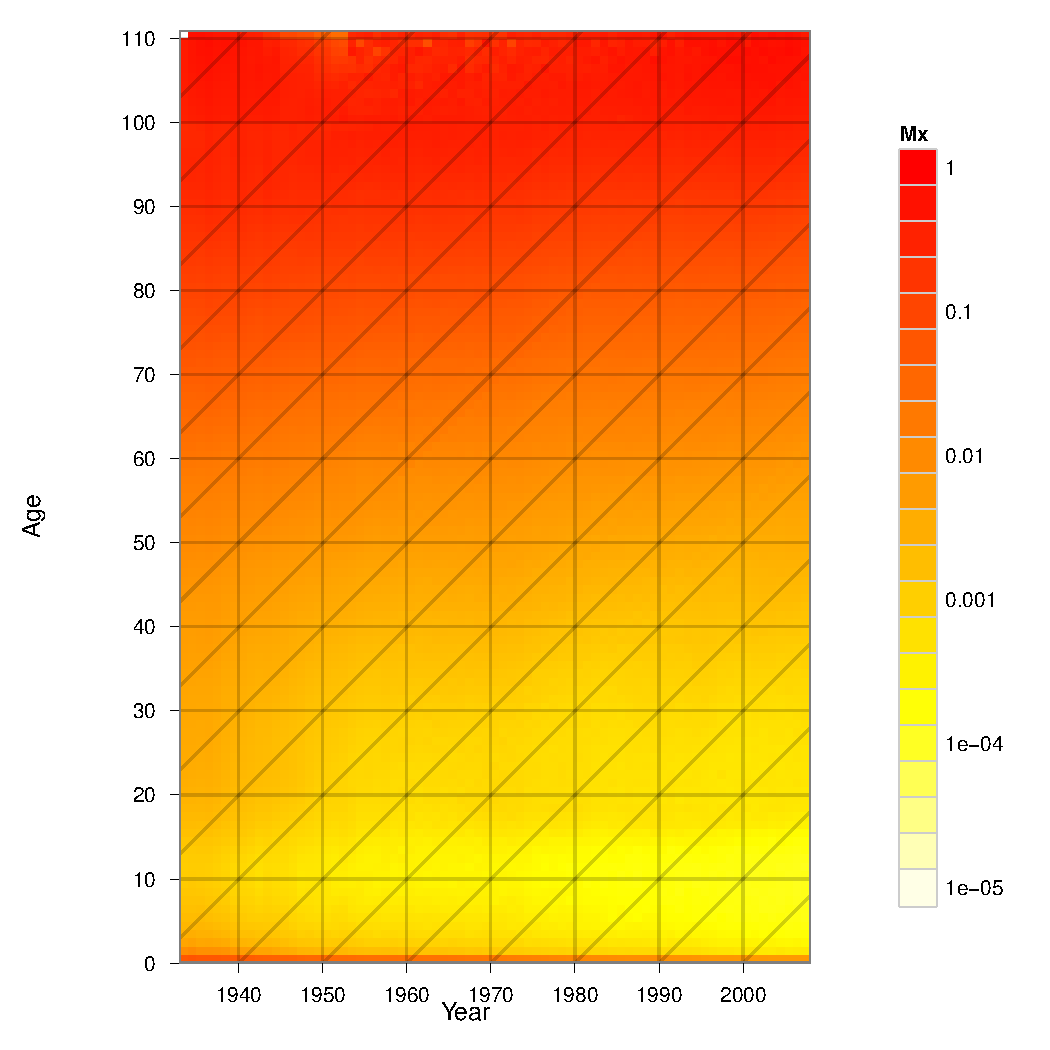
\includegraphics[width=4.5in,height=4.5in]{figs/ggplot2surface.pdf}
\caption{\texttt{ggplot()} function, tweaked to produce a Lexis surface.}
\end{figure}

Again, if anyone looks much into \texttt{ggplot2} and thinks they can improve this, pleaes let me know!
\subsection{PlotLexisTriangles()}
Some of you might be lucky enough to have data available in age-period-cohort format (Lexis triangles). The HMD\footnote{The HMD doesn't publish triangle exposures, just deaths, but you can still estimate them if needed.}, Kannisto-Thatcher database, and HFD are some places you can get data prepared in Lexis triangle format. Assuming you've got some data like that and you'd like to plot a true surface, you have few options (that I'm aware of) in R to plot the data \textit{as} triangles. So, a few months ago (summer 2011) I wrote a little (err, big) function that does just this. Here we'll walk through an example using Dutch APC rates from the HFD, including a few steps of pre-processing needed to get the data in the right format. First, sign up for the HFD if you haven't already \url{http://www.humanfertility.org}. I downloaded 2 files from this page: \url{http://www.humanfertility.org/cgi-bin/country.php?country=NLD&tab=asfr&t1=3&t2=4}, year, age, cohort Birth counts and year, age, cohort Female population exposure, which download as \texttt{NLDbirthsTR.txt} and \texttt{NLDexposTR.txt}, respectively.



\begin{Houtput}
\hspace*{\fill}\\
\hlstd{}\ttfamily\noindent
\hlprompt{\usebox{\hlnormalsizeboxgreaterthan}{\ }}\hlsymbol{B}{\ }\hlassignement{\usebox{\hlnormalsizeboxlessthan}-}{\ }\hlfunctioncall{read.table}\hlkeyword{(}\hlstring{"data/NLDbirthsTR.txt"}\hlkeyword{,}{\ }\hlargument{header}{\ }\hlargument{=}{\ }\hlnumber{TRUE}\hlkeyword{,}\hspace*{\fill}\\
\hlstd{}\hlprompt{{\ }}{\ }{\ }{\ }{\ }\hlargument{skip}{\ }\hlargument{=}{\ }\hlnumber{2}\hlkeyword{,}{\ }\hlargument{na.strings}{\ }\hlargument{=}{\ }\hlstring{"."}\hlkeyword{,}{\ }\hlargument{as.is}{\ }\hlargument{=}{\ }\hlnumber{TRUE}\hlkeyword{)}\mbox{}
\normalfont
\hspace*{\fill}\\
\hlstd{}\ttfamily\noindent
\hlprompt{\usebox{\hlnormalsizeboxgreaterthan}{\ }}\hlsymbol{E}{\ }\hlassignement{\usebox{\hlnormalsizeboxlessthan}-}{\ }\hlfunctioncall{read.table}\hlkeyword{(}\hlstring{"data/NLDexposTR.txt"}\hlkeyword{,}{\ }\hlargument{header}{\ }\hlargument{=}{\ }\hlnumber{TRUE}\hlkeyword{,}\hspace*{\fill}\\
\hlstd{}\hlprompt{{\ }}{\ }{\ }{\ }{\ }\hlargument{skip}{\ }\hlargument{=}{\ }\hlnumber{2}\hlkeyword{,}{\ }\hlargument{na.strings}{\ }\hlargument{=}{\ }\hlstring{"."}\hlkeyword{,}{\ }\hlargument{as.is}{\ }\hlargument{=}{\ }\hlnumber{TRUE}\hlkeyword{)}\mbox{}
\normalfont
\hspace*{\fill}\\
\hlstd{}\ttfamily\noindent
\hlprompt{\usebox{\hlnormalsizeboxgreaterthan}{\ }}\hlfunctioncall{head}\hlkeyword{(}\hlsymbol{B}\hlkeyword{)}\mbox{}
\normalfont
\hspace*{\fill}\\
\hlstd{}\begin{Schunk}
\begin{Soutput}
  Year Age Cohort Total
1 1950 12-     NA  0.03
2 1950  13   1937  0.16
3 1950  13   1936  0.39
4 1950  14   1936  2.21
5 1950  14   1935  4.22
6 1950  15   1935 14.00
\end{Soutput}
\ttfamily\noindent
\hlprompt{\usebox{\hlnormalsizeboxgreaterthan}{\ }}\hlfunctioncall{head}\hlkeyword{(}\hlsymbol{E}\hlkeyword{)}\mbox{}
\normalfont
\hspace*{\fill}\\
\hlstd{}\begin{Soutput}
  Year Age Cohort Exposure
1 1950  12   1938 41900.49
2 1950  12   1937 38499.18
3 1950  13   1937 39838.81
4 1950  13   1936 38822.81
5 1950  14   1936 39796.44
6 1950  14   1935 37950.91
\end{Soutput}
\ttfamily\noindent
\hlprompt{\usebox{\hlnormalsizeboxgreaterthan}{\ }}\hlcomment{\usebox{\hlnormalsizeboxhash}{\ }cut{\ }out{\ }open{\ }ages,{\ }match{\ }dimensions}\mbox{}
\normalfont
\hspace*{\fill}\\
\hlstd{}\ttfamily\noindent
\hlprompt{\usebox{\hlnormalsizeboxgreaterthan}{\ }}\hlsymbol{B}{\ }\hlassignement{\usebox{\hlnormalsizeboxlessthan}-}{\ }\hlsymbol{B}\hlkeyword{[}\hlsymbol{B}\hlkeyword{\usebox{\hlnormalsizeboxdollar}}\hlsymbol{Age}{\ }\hlkeyword{!=}{\ }\hlstring{"12-"}{\ }\hlkeyword{\usebox{\hlnormalsizeboxand}}{\ }\hlsymbol{B}\hlkeyword{\usebox{\hlnormalsizeboxdollar}}\hlsymbol{Age}{\ }\hlkeyword{!=}{\ }\hlstring{"55+"}\hlkeyword{,}{\ }\hlkeyword{]}\mbox{}
\normalfont
\hspace*{\fill}\\
\hlstd{}\ttfamily\noindent
\hlprompt{\usebox{\hlnormalsizeboxgreaterthan}{\ }}\hlsymbol{E}{\ }\hlassignement{\usebox{\hlnormalsizeboxlessthan}-}{\ }\hlsymbol{E}\hlkeyword{[}\hlsymbol{E}\hlkeyword{\usebox{\hlnormalsizeboxdollar}}\hlsymbol{Age}{\ }\hlkeyword{!=}{\ }\hlnumber{12}{\ }\hlkeyword{\usebox{\hlnormalsizeboxand}}{\ }\hlsymbol{E}\hlkeyword{\usebox{\hlnormalsizeboxdollar}}\hlsymbol{Age}{\ }\hlkeyword{!=}{\ }\hlnumber{55}\hlkeyword{,}{\ }\hlkeyword{]}\mbox{}
\normalfont
\hspace*{\fill}\\
\hlstd{}\ttfamily\noindent
\hlprompt{\usebox{\hlnormalsizeboxgreaterthan}{\ }}\hlsymbol{Ages}{\ }\hlassignement{\usebox{\hlnormalsizeboxlessthan}-}{\ }\hlnumber{13}\hlkeyword{:}\hlnumber{54}\mbox{}
\normalfont
\hspace*{\fill}\\
\hlstd{}\ttfamily\noindent
\hlprompt{\usebox{\hlnormalsizeboxgreaterthan}{\ }}\hlsymbol{Years}{\ }\hlassignement{\usebox{\hlnormalsizeboxlessthan}-}{\ }\hlfunctioncall{unique}\hlkeyword{(}\hlsymbol{B}\hlkeyword{\usebox{\hlnormalsizeboxdollar}}\hlsymbol{Year}\hlkeyword{)}\mbox{}
\normalfont
\hspace*{\fill}\\
\hlstd{}
\end{Schunk}
\end{Houtput}

Just as a convenience in this case, we cut off the open ages groups for ages 12 and under and 55 and over. This fertility surface will then cover ages 13 to 54 and years 1950 to 2009. The next step involves splitting the data into two matrices, one for upper triangles and another for lower triangles- this we only do because I wrote the function to take matrix objects \texttt{UpperTriangles} and \texttt{LowerTriangles} as primary arguments\footnote{In the future this might be modified to take data as-is and figure out the triangles on its own}. In our case, odd-numered rows correspond with lower triangles and even-numbered rows correspond with upper triangles. The code bit $\texttt{(1:nrow(B)\%\%2)==1}$ means litarally, divide the row indices by 2 and tell me which have a \textit{remainder} (i.e. elementary school math before they teach you decimals) of 1. Really, $\texttt{seq(2,nrow(B),by=2)}$ would have given us the same thing. The next step is to reshape the data from a long \texttt{data.frame} into a wide \texttt{matrix}, then divide counts by exposures to get rates.

\begin{Houtput}
\hspace*{\fill}\\
\hlstd{}\ttfamily\noindent
\hlprompt{\usebox{\hlnormalsizeboxgreaterthan}{\ }}\hlcomment{\usebox{\hlnormalsizeboxhash}{\ }split{\ }into{\ }2{\ }matrices{\ }for{\ }upper{\ }(UB)and{\ }lower}\mbox{}
\normalfont
\hspace*{\fill}\\
\hlstd{}\ttfamily\noindent
\hlprompt{\usebox{\hlnormalsizeboxgreaterthan}{\ }}\hlcomment{\usebox{\hlnormalsizeboxhash}{\ }{\ }{\ }triangles(LB):}\mbox{}
\normalfont
\hspace*{\fill}\\
\hlstd{}\ttfamily\noindent
\hlprompt{\usebox{\hlnormalsizeboxgreaterthan}{\ }}\hlcomment{\usebox{\hlnormalsizeboxhash}{\ }LB{\ }={\ }lower{\ }births,{\ }odds}\mbox{}
\normalfont
\hspace*{\fill}\\
\hlstd{}\ttfamily\noindent
\hlprompt{\usebox{\hlnormalsizeboxgreaterthan}{\ }}\hlsymbol{LB}{\ }\hlassignement{\usebox{\hlnormalsizeboxlessthan}-}{\ }\hlsymbol{B}\hlkeyword{[}\hlkeyword{(}\hlnumber{1}\hlkeyword{:}\hlfunctioncall{nrow}\hlkeyword{(}\hlsymbol{B}\hlkeyword{)}\hlkeyword{\usebox{\hlnormalsizeboxpercent}\usebox{\hlnormalsizeboxpercent}}\hlnumber{2}\hlkeyword{)}{\ }=={\ }\hlnumber{1}\hlkeyword{,}{\ }\hlkeyword{]}\mbox{}
\normalfont
\hspace*{\fill}\\
\hlstd{}\ttfamily\noindent
\hlprompt{\usebox{\hlnormalsizeboxgreaterthan}{\ }}\hlcomment{\usebox{\hlnormalsizeboxhash}{\ }turn{\ }into{\ }matrix,{\ }years{\ }columns,{\ }ages{\ }rows}\mbox{}
\normalfont
\hspace*{\fill}\\
\hlstd{}\ttfamily\noindent
\hlprompt{\usebox{\hlnormalsizeboxgreaterthan}{\ }}\hlsymbol{LB}{\ }\hlassignement{\usebox{\hlnormalsizeboxlessthan}-}{\ }\hlfunctioncall{matrix}\hlkeyword{(}\hlsymbol{LB}\hlkeyword{[}\hlkeyword{,}{\ }\hlnumber{4}\hlkeyword{]}\hlkeyword{,}{\ }\hlargument{nrow}{\ }\hlargument{=}{\ }\hlfunctioncall{length}\hlkeyword{(}\hlsymbol{Ages}\hlkeyword{)}\hlkeyword{)}\mbox{}
\normalfont
\hspace*{\fill}\\
\hlstd{}\ttfamily\noindent
\hlprompt{\usebox{\hlnormalsizeboxgreaterthan}{\ }}\hlcomment{\usebox{\hlnormalsizeboxhash}{\ }upper{\ }births,{\ }evens}\mbox{}
\normalfont
\hspace*{\fill}\\
\hlstd{}\ttfamily\noindent
\hlprompt{\usebox{\hlnormalsizeboxgreaterthan}{\ }}\hlsymbol{UB}{\ }\hlassignement{\usebox{\hlnormalsizeboxlessthan}-}{\ }\hlsymbol{B}\hlkeyword{[}\hlkeyword{(}\hlnumber{1}\hlkeyword{:}\hlfunctioncall{nrow}\hlkeyword{(}\hlsymbol{B}\hlkeyword{)}\hlkeyword{\usebox{\hlnormalsizeboxpercent}\usebox{\hlnormalsizeboxpercent}}\hlnumber{2}\hlkeyword{)}{\ }=={\ }\hlnumber{0}\hlkeyword{,}{\ }\hlkeyword{]}\mbox{}
\normalfont
\hspace*{\fill}\\
\hlstd{}\ttfamily\noindent
\hlprompt{\usebox{\hlnormalsizeboxgreaterthan}{\ }}\hlsymbol{UB}{\ }\hlassignement{\usebox{\hlnormalsizeboxlessthan}-}{\ }\hlfunctioncall{matrix}\hlkeyword{(}\hlsymbol{UB}\hlkeyword{[}\hlkeyword{,}{\ }\hlnumber{4}\hlkeyword{]}\hlkeyword{,}{\ }\hlargument{nrow}{\ }\hlargument{=}{\ }\hlfunctioncall{length}\hlkeyword{(}\hlsymbol{Ages}\hlkeyword{)}\hlkeyword{)}\mbox{}
\normalfont
\hspace*{\fill}\\
\hlstd{}\ttfamily\noindent
\hlprompt{\usebox{\hlnormalsizeboxgreaterthan}{\ }}\hlcomment{\usebox{\hlnormalsizeboxhash}\usebox{\hlnormalsizeboxhash}\usebox{\hlnormalsizeboxhash}\usebox{\hlnormalsizeboxhash}\usebox{\hlnormalsizeboxhash}\usebox{\hlnormalsizeboxhash}\usebox{\hlnormalsizeboxhash}\usebox{\hlnormalsizeboxhash}\usebox{\hlnormalsizeboxhash}\usebox{\hlnormalsizeboxhash}\usebox{\hlnormalsizeboxhash}\usebox{\hlnormalsizeboxhash}\usebox{\hlnormalsizeboxhash}\usebox{\hlnormalsizeboxhash}\usebox{\hlnormalsizeboxhash}\usebox{\hlnormalsizeboxhash}\usebox{\hlnormalsizeboxhash}\usebox{\hlnormalsizeboxhash}\usebox{\hlnormalsizeboxhash}\usebox{\hlnormalsizeboxhash}\usebox{\hlnormalsizeboxhash}}\mbox{}
\normalfont
\hspace*{\fill}\\
\hlstd{}\ttfamily\noindent
\hlprompt{\usebox{\hlnormalsizeboxgreaterthan}{\ }}\hlcomment{\usebox{\hlnormalsizeboxhash}{\ }Exposures}\mbox{}
\normalfont
\hspace*{\fill}\\
\hlstd{}\ttfamily\noindent
\hlprompt{\usebox{\hlnormalsizeboxgreaterthan}{\ }}\hlsymbol{LE}{\ }\hlassignement{\usebox{\hlnormalsizeboxlessthan}-}{\ }\hlsymbol{E}\hlkeyword{[}\hlkeyword{(}\hlnumber{1}\hlkeyword{:}\hlfunctioncall{nrow}\hlkeyword{(}\hlsymbol{E}\hlkeyword{)}\hlkeyword{\usebox{\hlnormalsizeboxpercent}\usebox{\hlnormalsizeboxpercent}}\hlnumber{2}\hlkeyword{)}{\ }=={\ }\hlnumber{1}\hlkeyword{,}{\ }\hlkeyword{]}\mbox{}
\normalfont
\hspace*{\fill}\\
\hlstd{}\ttfamily\noindent
\hlprompt{\usebox{\hlnormalsizeboxgreaterthan}{\ }}\hlsymbol{UE}{\ }\hlassignement{\usebox{\hlnormalsizeboxlessthan}-}{\ }\hlsymbol{E}\hlkeyword{[}\hlkeyword{(}\hlnumber{1}\hlkeyword{:}\hlfunctioncall{nrow}\hlkeyword{(}\hlsymbol{E}\hlkeyword{)}\hlkeyword{\usebox{\hlnormalsizeboxpercent}\usebox{\hlnormalsizeboxpercent}}\hlnumber{2}\hlkeyword{)}{\ }=={\ }\hlnumber{0}\hlkeyword{,}{\ }\hlkeyword{]}\mbox{}
\normalfont
\hspace*{\fill}\\
\hlstd{}\ttfamily\noindent
\hlprompt{\usebox{\hlnormalsizeboxgreaterthan}{\ }}\hlsymbol{UE}{\ }\hlassignement{\usebox{\hlnormalsizeboxlessthan}-}{\ }\hlfunctioncall{matrix}\hlkeyword{(}\hlsymbol{UE}\hlkeyword{[}\hlkeyword{,}{\ }\hlnumber{4}\hlkeyword{]}\hlkeyword{,}{\ }\hlargument{nrow}{\ }\hlargument{=}{\ }\hlfunctioncall{length}\hlkeyword{(}\hlsymbol{Ages}\hlkeyword{)}\hlkeyword{)}\mbox{}
\normalfont
\hspace*{\fill}\\
\hlstd{}\ttfamily\noindent
\hlprompt{\usebox{\hlnormalsizeboxgreaterthan}{\ }}\hlsymbol{LE}{\ }\hlassignement{\usebox{\hlnormalsizeboxlessthan}-}{\ }\hlfunctioncall{matrix}\hlkeyword{(}\hlsymbol{LE}\hlkeyword{[}\hlkeyword{,}{\ }\hlnumber{4}\hlkeyword{]}\hlkeyword{,}{\ }\hlargument{nrow}{\ }\hlargument{=}{\ }\hlfunctioncall{length}\hlkeyword{(}\hlsymbol{Ages}\hlkeyword{)}\hlkeyword{)}\mbox{}
\normalfont
\hspace*{\fill}\\
\hlstd{}\ttfamily\noindent
\hlprompt{\usebox{\hlnormalsizeboxgreaterthan}{\ }}\hlcomment{\usebox{\hlnormalsizeboxhash}{\ }divide{\ }to{\ }get{\ }rates:}\mbox{}
\normalfont
\hspace*{\fill}\\
\hlstd{}\ttfamily\noindent
\hlprompt{\usebox{\hlnormalsizeboxgreaterthan}{\ }}\hlsymbol{UpperTriangles}{\ }\hlassignement{\usebox{\hlnormalsizeboxlessthan}-}{\ }\hlsymbol{UB}\hlkeyword{/}\hlsymbol{UE}\mbox{}
\normalfont
\hspace*{\fill}\\
\hlstd{}\ttfamily\noindent
\hlprompt{\usebox{\hlnormalsizeboxgreaterthan}{\ }}\hlsymbol{LowerTriangles}{\ }\hlassignement{\usebox{\hlnormalsizeboxlessthan}-}{\ }\hlsymbol{LB}\hlkeyword{/}\hlsymbol{LE}\mbox{}
\normalfont
\hspace*{\fill}\\
\hlstd{}\ttfamily\noindent
\hlprompt{\usebox{\hlnormalsizeboxgreaterthan}{\ }}\hlfunctioncall{rownames}\hlkeyword{(}\hlsymbol{UpperTriangles}\hlkeyword{)}{\ }\hlassignement{\usebox{\hlnormalsizeboxlessthan}-}{\ }\hlfunctioncall{rownames}\hlkeyword{(}\hlsymbol{LowerTriangles}\hlkeyword{)}{\ }\hlassignement{\usebox{\hlnormalsizeboxlessthan}-}{\ }\hlsymbol{Ages}\mbox{}
\normalfont
\hspace*{\fill}\\
\hlstd{}\ttfamily\noindent
\hlprompt{\usebox{\hlnormalsizeboxgreaterthan}{\ }}\hlfunctioncall{colnames}\hlkeyword{(}\hlsymbol{LowerTriangles}\hlkeyword{)}{\ }\hlassignement{\usebox{\hlnormalsizeboxlessthan}-}{\ }\hlfunctioncall{colnames}\hlkeyword{(}\hlsymbol{LowerTriangles}\hlkeyword{)}{\ }\hlassignement{\usebox{\hlnormalsizeboxlessthan}-}{\ }\hlsymbol{Years}\mbox{}
\normalfont
\hspace*{\fill}\\
\hlstd{}
\end{Houtput}

The package \texttt{LexisSurface} is not on CRAN\footnote{yet! The default legend needs to be improved, and after that it'll be ready.}, but I included the zipped package in the data folder for this tutorial. You can do a local install from syntax using $\texttt{install.packages("data/LexisSurface\textunderscore 1.1.zip",repos=NULL)}$, changing the path as needed. We then load the package and invent a color ramp for fertility, \texttt{myFxcols()}. The legend color strip needs to be told explicitly where to go, using the pattern \texttt{c(xmin,ymin,xmax,ymax)}, and we tell the function to overplot lexis reference lines at 5-year intervals. APC mortality surfaces would be plotted in much the same way, except you would specify $\texttt{log=TRUE}$ and move the legend to somewhere convenient.

\begin{Houtput}
\hspace*{\fill}\\
\hlstd{}\ttfamily\noindent
\hlprompt{\usebox{\hlnormalsizeboxgreaterthan}{\ }}\hlcomment{\usebox{\hlnormalsizeboxhash}install.packages(\usebox{\hlnormalsizeboxsinglequote}data/LexisSurface\usebox{\hlnormalsizeboxunderscore}1.1.zip\usebox{\hlnormalsizeboxsinglequote})}\mbox{}
\normalfont
\hspace*{\fill}\\
\hlstd{}\ttfamily\noindent
\hlprompt{\usebox{\hlnormalsizeboxgreaterthan}{\ }}\hlfunctioncall{library}\hlkeyword{(}\hlsymbol{LexisSurface}\hlkeyword{)}\mbox{}
\normalfont
\hspace*{\fill}\\
\hlstd{}\ttfamily\noindent
\hlprompt{\usebox{\hlnormalsizeboxgreaterthan}{\ }}\hlcomment{\usebox{\hlnormalsizeboxhash}{\ }invent{\ }Fx{\ }color{\ }ramp{\ }(any{\ }suggestions{\ }for{\ }better?)}\mbox{}
\normalfont
\hspace*{\fill}\\
\hlstd{}\ttfamily\noindent
\hlprompt{\usebox{\hlnormalsizeboxgreaterthan}{\ }}\hlsymbol{myFxcols}{\ }\hlassignement{\usebox{\hlnormalsizeboxlessthan}-}{\ }\hlpackage{grDevices}\hlkeyword{:::}\hlfunctioncall{colorRampPalette}\hlkeyword{(}\hlfunctioncall{c}\hlkeyword{(}\hlstring{"white"}\hlkeyword{,}\hspace*{\fill}\\
\hlstd{}\hlprompt{{\ }}{\ }{\ }{\ }{\ }\hlstring{"blue"}\hlkeyword{,}{\ }\hlstring{"green"}\hlkeyword{,}{\ }\hlstring{"yellow"}\hlkeyword{,}{\ }\hlstring{"orange"}\hlkeyword{)}\hlkeyword{,}{\ }\hlargument{space}{\ }\hlargument{=}{\ }\hlstring{"rgb"}\hlkeyword{)}\mbox{}
\normalfont
\hspace*{\fill}\\
\hlstd{}
\end{Houtput}

\begin{Houtput}
\hspace*{\fill}\\
\hlstd{}\ttfamily\noindent
\hlprompt{\usebox{\hlnormalsizeboxgreaterthan}{\ }}\hlfunctioncall{PlotLexisTriangles}\hlkeyword{(}\hlsymbol{UpperTriangles}\hlkeyword{,}{\ }\hlsymbol{LowerTriangles}\hlkeyword{,}\hspace*{\fill}\\
\hlstd{}\hlprompt{{\ }}{\ }{\ }{\ }{\ }\hlargument{colorramp}{\ }\hlargument{=}{\ }\hlsymbol{myFxcols}\hlkeyword{,}{\ }\hlargument{log}{\ }\hlargument{=}{\ }\hlnumber{FALSE}\hlkeyword{,}{\ }\hlargument{lex.line.int}{\ }\hlargument{=}{\ }\hlnumber{5}\hlkeyword{,}{\ }\hlargument{main}{\ }\hlargument{=}{\ }\hlstring{"APC{\ }Fertility{\ }Rates,{\ }NE,{\ }1950-2009,{\ }HFD"}\hlkeyword{,}\hspace*{\fill}\\
\hlstd{}\hlprompt{{\ }}{\ }{\ }{\ }{\ }\hlargument{leg.coords}{\ }\hlargument{=}{\ }\hlfunctioncall{c}\hlkeyword{(}\hlnumber{1960}\hlkeyword{,}{\ }\hlnumber{2}\hlkeyword{,}{\ }\hlnumber{1999}\hlkeyword{,}{\ }\hlnumber{4}\hlkeyword{)}\hlkeyword{)}\mbox{}
\normalfont
\hspace*{\fill}\\
\hlstd{}
\end{Houtput}



\begin{figure}[H]
\centering
\includegraphics[width=4.5in,height=4.5in]{figs/lextri.pdf}
\caption{Fertility surface with PlotLexisTriangles() function.}
\end{figure}

The insides of this function are based almost entirely on the primitive \texttt{polygon()} and \texttt{segments()} functions. It would be possible to write a function to do the same thing using \texttt{lattice} conventions, and it's likely possible in \texttt{ggplot2}, though I'm still looking into this. Neither of those possible variants will be further explored.

\pagebreak
\section{Population pyramids}
By now you will probably have seen how to make populatin pyramids in Excel, but it's well worth your time to see a couple R-tastic ways of making them as well because 1) it's faster! 2) they are easier to standardize and make comparable and 3) it's way more reproducible. You might disagree with the first point, but actually if you already have your data in the shape required by Excel, then you have a few R functions at your disposal to make the pyramid in a single step. I'll present 2 functions, \texttt{pyramid} from the \texttt{pyramid} package by Minato Nakazawa and my own \texttt{Pyramid} function in the package \texttt{Pyramid}. For your information, there is also a pyramid plotting functions in the \texttt{plotrix} package, and there maybe others on CRAN as well. I show them both because they differ essentially in their plotting strategy. \texttt{Pyramid()} wraps directly to \texttt{barplot()} from base graphics, whereas \texttt{pyramid()} calls the even more primitive \texttt{polygon()} function. The plot aesthetics are also a bit different between the two functions.\\

First some words on population pyramids in general: There are a set of conventions that one must adhere to, just as for Lexis surfaces, in order that population pyramids be correctly interpreted and comparable between populations. First and always: use equal axis extremes for males and females so that the pyramid is centered in your figure. If you are doing multiple pyramids, think carefully about the kind of comparisons you'll want to do. This will bear directly on your decision for x-axis limits. For two populations of similar size, it is OK to use absolute population counts for the axes as long as the axes are the same for both figures and both pyramids are still intelligible. In this way you can get an idea of cohort sizes and population structure at the same time. This circumstance will rarely pertain in reality. If two populations are of different orders of size (or even if one is just 20\% bigger than the other), and you are even remotely interested in comparing population structure then you should rescale the populations before plotting. What number to rescale to is a matter of choice, but 100 is a decent choice, such that the x axis ticks can be clean percentages. You'll typically have 2 vectors of numbers, one for male counts by age and another for female counts by age: Rescaling must be done in terms of the sum of \textit{both} of these vectors together, not separately. There will be an example of theis pre-plotting step for the \texttt{pyramid()} function (\texttt{Pyramid()} does it automagically). Take home message: pyramids are for looking at structure, and are best looked at and compared on the same scale. Finally (and never forget it!), males on the left, females on the right\footnote{I once saw a famous French demographer do just the opposite, and this person failed to point out the fact. Of course you always need to adhere to local standards, but do be aware that most demographer around the world put males on the left.}. This last is in my opinion just as important as always plotting cohort lines at 45 degree angles. Just do it.\\

For both functions, we'll use Spanish data from the year 2000 \footnote{These are included in \texttt{Pyramid} package as examples data} from the HMD.

\begin{Houtput}
\hspace*{\fill}\\
\hlstd{}\ttfamily\noindent
\hlprompt{\usebox{\hlnormalsizeboxgreaterthan}{\ }}\hlsymbol{ESP2000}{\ }\hlassignement{\usebox{\hlnormalsizeboxlessthan}-}{\ }\hlfunctioncall{read.table}\hlkeyword{(}\hlstring{"data/ES2000.txt"}\hlkeyword{,}{\ }\hlargument{sep}{\ }\hlargument{=}{\ }\hlstring{"\usebox{\hlnormalsizeboxbackslash}t"}\hlkeyword{,}\hspace*{\fill}\\
\hlstd{}\hlprompt{{\ }}{\ }{\ }{\ }{\ }\hlargument{header}{\ }\hlargument{=}{\ }\hlnumber{TRUE}\hlkeyword{)}\mbox{}
\normalfont
\hspace*{\fill}\\
\hlstd{}\ttfamily\noindent
\hlprompt{\usebox{\hlnormalsizeboxgreaterthan}{\ }}\hlfunctioncall{rownames}\hlkeyword{(}\hlsymbol{ESP2000}\hlkeyword{)}{\ }\hlassignement{\usebox{\hlnormalsizeboxlessthan}-}{\ }\hlnumber{0}\hlkeyword{:}\hlnumber{110}\mbox{}
\normalfont
\hspace*{\fill}\\
\hlstd{}\ttfamily\noindent
\hlprompt{\usebox{\hlnormalsizeboxgreaterthan}{\ }}\hlfunctioncall{head}\hlkeyword{(}\hlsymbol{ESP2000}\hlkeyword{)}\mbox{}
\normalfont
\hspace*{\fill}\\
\hlstd{}\begin{Schunk}
\begin{Soutput}
   males females
0 195176  183999
1 188275  177464
2 187834  177790
3 186656  176754
4 188114  178140
5 191968  181515
\end{Soutput}

\end{Schunk}
\end{Houtput}

\subsection{pyramid()}
The \texttt{pyramid()} function takes a \texttt{data.frame} as it's primary argument\footnote{the same package also offers \texttt{pyramids()}, which takes vector arguments.}. This needs to have at least 2 columns, the first for the left side of the pyramid (males in our convention) and the second for the right side (females). Ages are either taken from the rownames or from an optional third column in the \texttt{data.frame}.

\begin{Houtput}
\hspace*{\fill}\\
\hlstd{}\ttfamily\noindent
\hlprompt{\usebox{\hlnormalsizeboxgreaterthan}{\ }}\hlcomment{\usebox{\hlnormalsizeboxhash}{\ }install{\ }from{\ }CRAN{\ }if{\ }needed:}\mbox{}
\normalfont
\hspace*{\fill}\\
\hlstd{}\ttfamily\noindent
\hlprompt{\usebox{\hlnormalsizeboxgreaterthan}{\ }}\hlcomment{\usebox{\hlnormalsizeboxhash}install.packages(\usebox{\hlnormalsizeboxsinglequote}pyramid\usebox{\hlnormalsizeboxsinglequote},lib=\usebox{\hlnormalsizeboxsinglequote}C:/Program}\mbox{}
\normalfont
\hspace*{\fill}\\
\hlstd{}\ttfamily\noindent
\hlprompt{\usebox{\hlnormalsizeboxgreaterthan}{\ }}\hlcomment{\usebox{\hlnormalsizeboxhash}{\ }{\ }{\ }Files/R/R-2.14.0/library\usebox{\hlnormalsizeboxsinglequote})}\mbox{}
\normalfont
\hspace*{\fill}\\
\hlstd{}\ttfamily\noindent
\hlprompt{\usebox{\hlnormalsizeboxgreaterthan}{\ }}\hlfunctioncall{source}\hlkeyword{(}\hlstring{"http://bioconductor.org/biocLite.R"}\hlkeyword{)}\mbox{}
\normalfont
\hspace*{\fill}\\
\hlstd{}\ttfamily\noindent
\hlprompt{\usebox{\hlnormalsizeboxgreaterthan}{\ }}\hlfunctioncall{biocLite}\hlkeyword{(}\hlstring{"pyramid"}\hlkeyword{,}{\ }\hlargument{ask}{\ }\hlargument{=}{\ }\hlnumber{FALSE}\hlkeyword{,}{\ }\hlargument{suppressUpdates}{\ }\hlargument{=}{\ }\hlnumber{TRUE}\hlkeyword{)}\mbox{}
\normalfont
\hspace*{\fill}\\
\hlstd{}\begin{Schunk}
\begin{Soutput}
package 'pyramid' successfully unpacked and MD5 sums checked

The downloaded packages are in
	C:\Users\triffe\AppData\Local\Temp\Rtmp6vwjKV\downloaded_packages
\end{Soutput}
\ttfamily\noindent
\hlprompt{\usebox{\hlnormalsizeboxgreaterthan}{\ }}\hlfunctioncall{library}\hlkeyword{(}\hlsymbol{pyramid}\hlkeyword{)}\mbox{}
\normalfont
\hspace*{\fill}\\
\hlstd{}\ttfamily\noindent
\hlprompt{\usebox{\hlnormalsizeboxgreaterthan}{\ }}\hlcomment{\usebox{\hlnormalsizeboxhash}{\ }convert{\ }to{\ }data.frame}\mbox{}
\normalfont
\hspace*{\fill}\\
\hlstd{}\ttfamily\noindent
\hlprompt{\usebox{\hlnormalsizeboxgreaterthan}{\ }}\hlsymbol{ESP2000df}{\ }\hlassignement{\usebox{\hlnormalsizeboxlessthan}-}{\ }\hlfunctioncall{as.data.frame}\hlkeyword{(}\hlsymbol{ESP2000}\hlkeyword{)}\mbox{}
\normalfont
\hspace*{\fill}\\
\hlstd{}
\end{Schunk}
\end{Houtput}

\begin{Houtput}
\hspace*{\fill}\\
\hlstd{}\ttfamily\noindent
\hlprompt{\usebox{\hlnormalsizeboxgreaterthan}{\ }}\hlfunctioncall{pyramid}\hlkeyword{(}\hlsymbol{ESP2000df}\hlkeyword{,}{\ }\hlargument{Llab}{\ }\hlargument{=}{\ }\hlstring{"Males"}\hlkeyword{,}{\ }\hlargument{Rlab}{\ }\hlargument{=}{\ }\hlstring{"Females"}\hlkeyword{,}\hspace*{\fill}\\
\hlstd{}\hlprompt{{\ }}{\ }{\ }{\ }{\ }\hlargument{Clab}{\ }\hlargument{=}{\ }\hlstring{""}\hlkeyword{,}{\ }\hlargument{Laxis}{\ }\hlargument{=}{\ }\hlfunctioncall{seq}\hlkeyword{(}\hlnumber{0}\hlkeyword{,}{\ }\hlnumber{350000}\hlkeyword{,}{\ }\hlargument{len}{\ }\hlargument{=}{\ }\hlnumber{5}\hlkeyword{)}\hlkeyword{,}{\ }\hlargument{AxisFM}{\ }\hlargument{=}{\ }\hlstring{"d"}\hlkeyword{,}\hspace*{\fill}\\
\hlstd{}\hlprompt{{\ }}{\ }{\ }{\ }{\ }\hlargument{AxisBM}{\ }\hlargument{=}{\ }\hlstring{","}\hlkeyword{,}{\ }\hlargument{Csize}{\ }\hlargument{=}{\ }\hlnumber{0.5}\hlkeyword{,}{\ }\hlargument{Cstep}{\ }\hlargument{=}{\ }\hlnumber{10}\hlkeyword{,}{\ }\hlargument{main}{\ }\hlargument{=}{\ }\hlstring{"Population{\ }pyramid{\ }of{\ }Spain\usebox{\hlnormalsizeboxbackslash}n{\ }(Data:{\ }HMD)"}\hlkeyword{)}\mbox{}
\normalfont
\hspace*{\fill}\\
\hlstd{}
\end{Houtput}

Some prefer the age axis to go up the middle, as is the standard with \texttt{pyramid()}. In this case the axis labels are a bit sloppy, and the function unfortunately offers no control over this at this time. I think we can get around that problem by simply rescaling the population prior to plotting (next step)



\begin{figure}[H]
\centering
\includegraphics[width=4.5in,height=4.5in]{figs/pyramid1.pdf}
\caption{\texttt{pyramid()}, with unscaled population.}
\end{figure}


Rescaling in R is super easy, just divide the thing by its own sum and multiply by whatever you want the new sum to be. In this case I multiply by 100 so that the age bars canbe thought of as percents (or fractions of percents).

\begin{Houtput}
\hspace*{\fill}\\
\hlstd{}\ttfamily\noindent
\hlprompt{\usebox{\hlnormalsizeboxgreaterthan}{\ }}\hlcomment{\usebox{\hlnormalsizeboxhash}{\ }rescale{\ }to{\ }100}\mbox{}
\normalfont
\hspace*{\fill}\\
\hlstd{}\ttfamily\noindent
\hlprompt{\usebox{\hlnormalsizeboxgreaterthan}{\ }}\hlsymbol{ESP2000df}{\ }\hlassignement{\usebox{\hlnormalsizeboxlessthan}-}{\ }\hlnumber{100}{\ }\hlkeyword{*}{\ }\hlkeyword{(}\hlsymbol{ESP2000df}\hlkeyword{/}\hlfunctioncall{sum}\hlkeyword{(}\hlsymbol{ESP2000df}\hlkeyword{)}\hlkeyword{)}\mbox{}
\normalfont
\hspace*{\fill}\\
\hlstd{}
\end{Houtput}

We have to change the lower axis limits. Replotting with essentially the same function call:

\begin{Houtput}
\hspace*{\fill}\\
\hlstd{}\ttfamily\noindent
\hlprompt{\usebox{\hlnormalsizeboxgreaterthan}{\ }}\hlfunctioncall{pyramid}\hlkeyword{(}\hlsymbol{ESP2000df}\hlkeyword{,}{\ }\hlargument{Llab}{\ }\hlargument{=}{\ }\hlstring{"Males"}\hlkeyword{,}{\ }\hlargument{Rlab}{\ }\hlargument{=}{\ }\hlstring{"Females"}\hlkeyword{,}\hspace*{\fill}\\
\hlstd{}\hlprompt{{\ }}{\ }{\ }{\ }{\ }\hlargument{Clab}{\ }\hlargument{=}{\ }\hlstring{""}\hlkeyword{,}{\ }\hlargument{Laxis}{\ }\hlargument{=}{\ }\hlfunctioncall{c}\hlkeyword{(}\hlnumber{0}\hlkeyword{,}{\ }\hlnumber{0.2}\hlkeyword{,}{\ }\hlnumber{0.4}\hlkeyword{,}{\ }\hlnumber{0.6}\hlkeyword{,}{\ }\hlnumber{0.8}\hlkeyword{,}{\ }\hlnumber{1}\hlkeyword{)}\hlkeyword{,}{\ }\hlargument{Cstep}{\ }\hlargument{=}{\ }\hlnumber{10}\hlkeyword{,}\hspace*{\fill}\\
\hlstd{}\hlprompt{{\ }}{\ }{\ }{\ }{\ }\hlargument{main}{\ }\hlargument{=}{\ }\hlstring{"Population{\ }pyramid{\ }of{\ }Spain\usebox{\hlnormalsizeboxbackslash}n{\ }(Data:{\ }HMD)"}\hlkeyword{)}\mbox{}
\normalfont
\hspace*{\fill}\\
\hlstd{}
\end{Houtput}



\begin{figure}[H]
\centering
\includegraphics[width=4.5in,height=4.5in]{figs/pyramid2.pdf}
\caption{\texttt{pyramid()}, with unscaled population.}
\end{figure}

I find the function rather inflexible in terms of labelling: it'd be nice to be able to add \% signs to the axis labels, and for the default axes to use clean numbers, but otherwise it does the job right. You can, for instance, adjust the spacing of the middle. Tick marks would be nice for the ages as well.

\subsection{Pyramid()}
The \texttt{Pyramid()} function takes care of several of these shortcomings, and has its own different set of defaults. The left axis labels are for ages and the right axis labels are for generations. Data are by default rescaled to percent (argument $\texttt{prop = TRUE}$). In order for the generations to calculate right, you need to specify the data year in the arguments, although the default year and the data year in this case (2000) coincide. 



\begin{Houtput}
\hspace*{\fill}\\
\hlstd{}\ttfamily\noindent
\hlprompt{\usebox{\hlnormalsizeboxgreaterthan}{\ }}\hlcomment{\usebox{\hlnormalsizeboxhash}{\ }library(Pyramid)}\mbox{}
\normalfont
\hspace*{\fill}\\
\hlstd{}\ttfamily\noindent
\hlprompt{\usebox{\hlnormalsizeboxgreaterthan}{\ }}\hlfunctioncall{Pyramid}\hlkeyword{(}\hlsymbol{ESP2000}\hlkeyword{[}\hlkeyword{,}{\ }\hlstring{"males"}\hlkeyword{]}\hlkeyword{,}{\ }\hlsymbol{ESP2000}\hlkeyword{[}\hlkeyword{,}{\ }\hlstring{"females"}\hlkeyword{]}\hlkeyword{,}\hspace*{\fill}\\
\hlstd{}\hlprompt{{\ }}{\ }{\ }{\ }{\ }\hlargument{widths}{\ }\hlargument{=}{\ }\hlfunctioncall{rep}\hlkeyword{(}\hlnumber{1}\hlkeyword{,}{\ }\hlnumber{111}\hlkeyword{)}\hlkeyword{)}\mbox{}
\normalfont
\hspace*{\fill}\\
\hlstd{}
\end{Houtput}



\begin{figure}[H]
\centering
\includegraphics[width=4.5in,height=4.5in]{figs/Pyramid3.pdf}
\caption{\texttt{Pyramid()}, leaving all defaults.}
\end{figure}

Nearly all aspects of the pyramid can be adjusted from the arguments, for instance for abridged 5-year age groups (with the \texttt{widths} argument), the colors, bars, reference lines, whether or not to plot generations, and so forth. In following, the same pyramid with several specified arguments:

\begin{Houtput}
\hspace*{\fill}\\
\hlstd{}\ttfamily\noindent
\hlprompt{\usebox{\hlnormalsizeboxgreaterthan}{\ }}\hlfunctioncall{Pyramid}\hlkeyword{(}\hlargument{males}{\ }\hlargument{=}{\ }\hlsymbol{ESP2000}\hlkeyword{[}\hlkeyword{,}{\ }\hlnumber{1}\hlkeyword{]}\hlkeyword{,}{\ }\hlargument{females}{\ }\hlargument{=}{\ }\hlsymbol{ESP2000}\hlkeyword{[}\hlkeyword{,}\hspace*{\fill}\\
\hlstd{}\hlprompt{{\ }}{\ }{\ }{\ }{\ }\hlnumber{2}\hlkeyword{]}\hlkeyword{,}{\ }\hlargument{border.males}{\ }\hlargument{=}{\ }\hlstring{"black"}\hlkeyword{,}{\ }\hlargument{border.females}{\ }\hlargument{=}{\ }\hlstring{"black"}\hlkeyword{,}{\ }\hlargument{fill.males}{\ }\hlargument{=}{\ }\hlstring{"cadetblue"}\hlkeyword{,}\hspace*{\fill}\\
\hlstd{}\hlprompt{{\ }}{\ }{\ }{\ }{\ }\hlargument{fill.females}{\ }\hlargument{=}{\ }\hlstring{"salmon"}\hlkeyword{,}{\ }\hlargument{gen.col}{\ }\hlargument{=}{\ }\hlstring{"\usebox{\hlnormalsizeboxhash}00000030"}\hlkeyword{,}{\ }\hlargument{year}{\ }\hlargument{=}{\ }\hlnumber{2000}\hlkeyword{,}\hspace*{\fill}\\
\hlstd{}\hlprompt{{\ }}{\ }{\ }{\ }{\ }\hlargument{main}{\ }\hlargument{=}{\ }\hlstring{"Spain{\ }population{\ }structure,{\ }year{\ }2000\usebox{\hlnormalsizeboxbackslash}ntotal{\ }population{\ }={\ }40.1{\ }million"}\hlkeyword{,}\hspace*{\fill}\\
\hlstd{}\hlprompt{{\ }}{\ }{\ }{\ }{\ }\hlargument{prop}{\ }\hlargument{=}{\ }\hlnumber{FALSE}\hlkeyword{,}{\ }\hlargument{widths}{\ }\hlargument{=}{\ }\hlfunctioncall{rep}\hlkeyword{(}\hlnumber{1}\hlkeyword{,}{\ }\hlnumber{111}\hlkeyword{)}\hlkeyword{)}\mbox{}
\normalfont
\hspace*{\fill}\\
\hlstd{}
\end{Houtput}



\begin{figure}[H]
\centering
\includegraphics[width=4.5in,height=4.5in]{figs/Pyramid4.pdf}
\caption{\texttt{Pyramid()}, adjusting several arguments.}
\end{figure}


Again, if comparing populations or the same population at different points in time, do two things: 1) Leave the default rescaling to percent and 2) set the \texttt{xlim} argument, just as you would for a normal plot. You would want, for instance, to fix the \texttt{xlim} argument if animating a population pyramid over a projection horizon, or a historical times series. This is a good way to get a feel for the concept of ergodicity. Refer to the following blog post for a guide to animating population pyramids in R \url{http://sites.google.com/site/timriffepersonal/DemogBlog/animatingapopulationpyramidinr}.\\\

\texttt{Pyramid()} also handles multistate population pyramids with no additional hassel. Multistate population pyramids are identical, but further subdivided into states such as marital states, health, employment, educational attainment, nationality, race, or any other state you might have information on in addition to age and sex. In this case, instead of specifying a vector, specify a matrix, where each column distinguishes a state, and specify the colors as vectors as well (one for each column). Here's a little example- I'll derive some fake states from the Spanish data just for the example plotting syntax:

\begin{Houtput}
\hspace*{\fill}\\
\hlstd{}\ttfamily\noindent
\hlprompt{\usebox{\hlnormalsizeboxgreaterthan}{\ }}\hlsymbol{m}{\ }\hlassignement{\usebox{\hlnormalsizeboxlessthan}-}{\ }\hlsymbol{ESP2000}\hlkeyword{[}\hlkeyword{,}{\ }\hlstring{"males"}\hlkeyword{]}\mbox{}
\normalfont
\hspace*{\fill}\\
\hlstd{}\ttfamily\noindent
\hlprompt{\usebox{\hlnormalsizeboxgreaterthan}{\ }}\hlsymbol{f}{\ }\hlassignement{\usebox{\hlnormalsizeboxlessthan}-}{\ }\hlsymbol{ESP2000}\hlkeyword{[}\hlkeyword{,}{\ }\hlstring{"females"}\hlkeyword{]}\mbox{}
\normalfont
\hspace*{\fill}\\
\hlstd{}\ttfamily\noindent
\hlprompt{\usebox{\hlnormalsizeboxgreaterthan}{\ }}\hlsymbol{pmales}{\ }\hlassignement{\usebox{\hlnormalsizeboxlessthan}-}{\ }\hlfunctioncall{c}\hlkeyword{(}\hlfunctioncall{rep}\hlkeyword{(}\hlnumber{0}\hlkeyword{,}{\ }\hlnumber{15}\hlkeyword{)}\hlkeyword{,}{\ }\hlfunctioncall{seq}\hlkeyword{(}\hlnumber{0}\hlkeyword{,}{\ }\hlnumber{0.7}\hlkeyword{,}{\ }\hlargument{length}{\ }\hlargument{=}{\ }\hlnumber{96}\hlkeyword{)}\hlkeyword{)}\mbox{}
\normalfont
\hspace*{\fill}\\
\hlstd{}\ttfamily\noindent
\hlprompt{\usebox{\hlnormalsizeboxgreaterthan}{\ }}\hlsymbol{pfemales}{\ }\hlassignement{\usebox{\hlnormalsizeboxlessthan}-}{\ }\hlsymbol{pmales}{\ }\hlkeyword{*}{\ }\hlnumber{0.9}\mbox{}
\normalfont
\hspace*{\fill}\\
\hlstd{}\ttfamily\noindent
\hlprompt{\usebox{\hlnormalsizeboxgreaterthan}{\ }}\hlsymbol{MalesMS}{\ }\hlassignement{\usebox{\hlnormalsizeboxlessthan}-}{\ }\hlfunctioncall{cbind}\hlkeyword{(}\hlsymbol{m}{\ }\hlkeyword{*}{\ }\hlsymbol{pmales}\hlkeyword{,}{\ }\hlsymbol{m}{\ }\hlkeyword{*}{\ }\hlkeyword{(}\hlnumber{1}{\ }\hlkeyword{-}{\ }\hlsymbol{pmales}\hlkeyword{)}\hlkeyword{)}\mbox{}
\normalfont
\hspace*{\fill}\\
\hlstd{}\ttfamily\noindent
\hlprompt{\usebox{\hlnormalsizeboxgreaterthan}{\ }}\hlsymbol{FemalesMS}{\ }\hlassignement{\usebox{\hlnormalsizeboxlessthan}-}{\ }\hlfunctioncall{cbind}\hlkeyword{(}\hlsymbol{f}{\ }\hlkeyword{*}{\ }\hlsymbol{pfemales}\hlkeyword{,}{\ }\hlsymbol{f}{\ }\hlkeyword{*}{\ }\hlkeyword{(}\hlnumber{1}{\ }\hlkeyword{-}{\ }\hlsymbol{pfemales}\hlkeyword{)}\hlkeyword{)}\mbox{}
\normalfont
\hspace*{\fill}\\
\hlstd{}\ttfamily\noindent
\hlprompt{\usebox{\hlnormalsizeboxgreaterthan}{\ }}\hlfunctioncall{colnames}\hlkeyword{(}\hlsymbol{MalesMS}\hlkeyword{)}{\ }\hlassignement{\usebox{\hlnormalsizeboxlessthan}-}{\ }\hlfunctioncall{c}\hlkeyword{(}\hlstring{"state{\ }1"}\hlkeyword{,}{\ }\hlstring{"state{\ }2"}\hlkeyword{)}\mbox{}
\normalfont
\hspace*{\fill}\\
\hlstd{}\ttfamily\noindent
\hlprompt{\usebox{\hlnormalsizeboxgreaterthan}{\ }}\hlfunctioncall{colnames}\hlkeyword{(}\hlsymbol{FemalesMS}\hlkeyword{)}{\ }\hlassignement{\usebox{\hlnormalsizeboxlessthan}-}{\ }\hlfunctioncall{c}\hlkeyword{(}\hlstring{"state{\ }1"}\hlkeyword{,}{\ }\hlstring{"state{\ }2"}\hlkeyword{)}\mbox{}
\normalfont
\hspace*{\fill}\\
\hlstd{}\ttfamily\noindent
\hlprompt{\usebox{\hlnormalsizeboxgreaterthan}{\ }}\hlfunctioncall{is.matrix}\hlkeyword{(}\hlsymbol{MalesMS}\hlkeyword{)}\mbox{}
\normalfont
\hspace*{\fill}\\
\hlstd{}\begin{Schunk}
\begin{Soutput}
[1] TRUE
\end{Soutput}

\end{Schunk}
\end{Houtput}

\begin{Houtput}
\hspace*{\fill}\\
\hlstd{}\ttfamily\noindent
\hlprompt{\usebox{\hlnormalsizeboxgreaterthan}{\ }}\hlfunctioncall{Pyramid}\hlkeyword{(}\hlargument{males}{\ }\hlargument{=}{\ }\hlsymbol{MalesMS}\hlkeyword{,}{\ }\hlargument{females}{\ }\hlargument{=}{\ }\hlsymbol{FemalesMS}\hlkeyword{,}{\ }\hlargument{border.males}{\ }\hlargument{=}{\ }\hlstring{"black"}\hlkeyword{,}\hspace*{\fill}\\
\hlstd{}\hlprompt{{\ }}{\ }{\ }{\ }{\ }\hlargument{border.females}{\ }\hlargument{=}{\ }\hlstring{"black"}\hlkeyword{,}{\ }\hlargument{fill.males}{\ }\hlargument{=}{\ }\hlfunctioncall{c}\hlkeyword{(}\hlstring{"skyblue2"}\hlkeyword{,}{\ }\hlstring{"orange"}\hlkeyword{)}\hlkeyword{,}\hspace*{\fill}\\
\hlstd{}\hlprompt{{\ }}{\ }{\ }{\ }{\ }\hlargument{fill.females}{\ }\hlargument{=}{\ }\hlfunctioncall{c}\hlkeyword{(}\hlstring{"skyblue2"}\hlkeyword{,}{\ }\hlstring{"orange"}\hlkeyword{)}\hlkeyword{,}{\ }\hlargument{gen.col}{\ }\hlargument{=}{\ }\hlstring{"\usebox{\hlnormalsizeboxhash}00000030"}\hlkeyword{,}\hspace*{\fill}\\
\hlstd{}\hlprompt{{\ }}{\ }{\ }{\ }{\ }\hlargument{year}{\ }\hlargument{=}{\ }\hlnumber{2000}\hlkeyword{,}{\ }\hlkeyword{,}{\ }\hlargument{widths}{\ }\hlargument{=}{\ }\hlfunctioncall{rep}\hlkeyword{(}\hlnumber{1}\hlkeyword{,}{\ }\hlnumber{111}\hlkeyword{)}\hlkeyword{,}{\ }\hlargument{main}{\ }\hlargument{=}{\ }\hlstring{"Spain{\ }multistate{\ }pop.{\ }structure,{\ }year{\ }2000\usebox{\hlnormalsizeboxbackslash}ntotal{\ }population{\ }={\ }40.1{\ }million"}\hlkeyword{)}\mbox{}
\normalfont
\hspace*{\fill}\\
\hlstd{}
\end{Houtput}



\begin{figure}[H]
\centering
\includegraphics[width=4.5in,height=4.5in]{figs/Pyramid5.pdf}
\caption{\texttt{Pyramid()}, for multistate population data.}
\end{figure}

There is no limit to the number of states you can introduce into the pyramid in this way (i.e. simply adding columns).

\nocite{*} % make sure all references included even if not explicitly in paper
\bibliographystyle{plainnat}
\bibliography{References}   % Use the BibTeX file ``References.bib''.

\end{document}
